% Generated by Sphinx.
\def\sphinxdocclass{report}
\documentclass[letterpaper,10pt,english]{sphinxmanual}
\usepackage[utf8]{inputenc}
\DeclareUnicodeCharacter{00A0}{\nobreakspace}
\usepackage{cmap}
\usepackage[T1]{fontenc}
\usepackage{babel}
\usepackage{times}
\usepackage[Bjarne]{fncychap}
\usepackage{longtable}
\usepackage{sphinx}
\usepackage{multirow}


\addto\captionsenglish{\renewcommand{\figurename}{Fig. }}
\addto\captionsenglish{\renewcommand{\tablename}{Table }}
\floatname{literal-block}{Listing }



\title{ClearMap Documentation}
\date{May 26, 2016}
\release{0.9.2}
\author{Christoph Kirst}
\newcommand{\sphinxlogo}{}
\renewcommand{\releasename}{Release}
\makeindex

\makeatletter
\def\PYG@reset{\let\PYG@it=\relax \let\PYG@bf=\relax%
    \let\PYG@ul=\relax \let\PYG@tc=\relax%
    \let\PYG@bc=\relax \let\PYG@ff=\relax}
\def\PYG@tok#1{\csname PYG@tok@#1\endcsname}
\def\PYG@toks#1+{\ifx\relax#1\empty\else%
    \PYG@tok{#1}\expandafter\PYG@toks\fi}
\def\PYG@do#1{\PYG@bc{\PYG@tc{\PYG@ul{%
    \PYG@it{\PYG@bf{\PYG@ff{#1}}}}}}}
\def\PYG#1#2{\PYG@reset\PYG@toks#1+\relax+\PYG@do{#2}}

\expandafter\def\csname PYG@tok@gd\endcsname{\def\PYG@tc##1{\textcolor[rgb]{0.63,0.00,0.00}{##1}}}
\expandafter\def\csname PYG@tok@gu\endcsname{\let\PYG@bf=\textbf\def\PYG@tc##1{\textcolor[rgb]{0.50,0.00,0.50}{##1}}}
\expandafter\def\csname PYG@tok@gt\endcsname{\def\PYG@tc##1{\textcolor[rgb]{0.00,0.27,0.87}{##1}}}
\expandafter\def\csname PYG@tok@gs\endcsname{\let\PYG@bf=\textbf}
\expandafter\def\csname PYG@tok@gr\endcsname{\def\PYG@tc##1{\textcolor[rgb]{1.00,0.00,0.00}{##1}}}
\expandafter\def\csname PYG@tok@cm\endcsname{\let\PYG@it=\textit\def\PYG@tc##1{\textcolor[rgb]{0.25,0.50,0.56}{##1}}}
\expandafter\def\csname PYG@tok@vg\endcsname{\def\PYG@tc##1{\textcolor[rgb]{0.73,0.38,0.84}{##1}}}
\expandafter\def\csname PYG@tok@m\endcsname{\def\PYG@tc##1{\textcolor[rgb]{0.13,0.50,0.31}{##1}}}
\expandafter\def\csname PYG@tok@mh\endcsname{\def\PYG@tc##1{\textcolor[rgb]{0.13,0.50,0.31}{##1}}}
\expandafter\def\csname PYG@tok@cs\endcsname{\def\PYG@tc##1{\textcolor[rgb]{0.25,0.50,0.56}{##1}}\def\PYG@bc##1{\setlength{\fboxsep}{0pt}\colorbox[rgb]{1.00,0.94,0.94}{\strut ##1}}}
\expandafter\def\csname PYG@tok@ge\endcsname{\let\PYG@it=\textit}
\expandafter\def\csname PYG@tok@vc\endcsname{\def\PYG@tc##1{\textcolor[rgb]{0.73,0.38,0.84}{##1}}}
\expandafter\def\csname PYG@tok@il\endcsname{\def\PYG@tc##1{\textcolor[rgb]{0.13,0.50,0.31}{##1}}}
\expandafter\def\csname PYG@tok@go\endcsname{\def\PYG@tc##1{\textcolor[rgb]{0.20,0.20,0.20}{##1}}}
\expandafter\def\csname PYG@tok@cp\endcsname{\def\PYG@tc##1{\textcolor[rgb]{0.00,0.44,0.13}{##1}}}
\expandafter\def\csname PYG@tok@gi\endcsname{\def\PYG@tc##1{\textcolor[rgb]{0.00,0.63,0.00}{##1}}}
\expandafter\def\csname PYG@tok@gh\endcsname{\let\PYG@bf=\textbf\def\PYG@tc##1{\textcolor[rgb]{0.00,0.00,0.50}{##1}}}
\expandafter\def\csname PYG@tok@ni\endcsname{\let\PYG@bf=\textbf\def\PYG@tc##1{\textcolor[rgb]{0.84,0.33,0.22}{##1}}}
\expandafter\def\csname PYG@tok@nl\endcsname{\let\PYG@bf=\textbf\def\PYG@tc##1{\textcolor[rgb]{0.00,0.13,0.44}{##1}}}
\expandafter\def\csname PYG@tok@nn\endcsname{\let\PYG@bf=\textbf\def\PYG@tc##1{\textcolor[rgb]{0.05,0.52,0.71}{##1}}}
\expandafter\def\csname PYG@tok@no\endcsname{\def\PYG@tc##1{\textcolor[rgb]{0.38,0.68,0.84}{##1}}}
\expandafter\def\csname PYG@tok@na\endcsname{\def\PYG@tc##1{\textcolor[rgb]{0.25,0.44,0.63}{##1}}}
\expandafter\def\csname PYG@tok@nb\endcsname{\def\PYG@tc##1{\textcolor[rgb]{0.00,0.44,0.13}{##1}}}
\expandafter\def\csname PYG@tok@nc\endcsname{\let\PYG@bf=\textbf\def\PYG@tc##1{\textcolor[rgb]{0.05,0.52,0.71}{##1}}}
\expandafter\def\csname PYG@tok@nd\endcsname{\let\PYG@bf=\textbf\def\PYG@tc##1{\textcolor[rgb]{0.33,0.33,0.33}{##1}}}
\expandafter\def\csname PYG@tok@ne\endcsname{\def\PYG@tc##1{\textcolor[rgb]{0.00,0.44,0.13}{##1}}}
\expandafter\def\csname PYG@tok@nf\endcsname{\def\PYG@tc##1{\textcolor[rgb]{0.02,0.16,0.49}{##1}}}
\expandafter\def\csname PYG@tok@si\endcsname{\let\PYG@it=\textit\def\PYG@tc##1{\textcolor[rgb]{0.44,0.63,0.82}{##1}}}
\expandafter\def\csname PYG@tok@s2\endcsname{\def\PYG@tc##1{\textcolor[rgb]{0.25,0.44,0.63}{##1}}}
\expandafter\def\csname PYG@tok@vi\endcsname{\def\PYG@tc##1{\textcolor[rgb]{0.73,0.38,0.84}{##1}}}
\expandafter\def\csname PYG@tok@nt\endcsname{\let\PYG@bf=\textbf\def\PYG@tc##1{\textcolor[rgb]{0.02,0.16,0.45}{##1}}}
\expandafter\def\csname PYG@tok@nv\endcsname{\def\PYG@tc##1{\textcolor[rgb]{0.73,0.38,0.84}{##1}}}
\expandafter\def\csname PYG@tok@s1\endcsname{\def\PYG@tc##1{\textcolor[rgb]{0.25,0.44,0.63}{##1}}}
\expandafter\def\csname PYG@tok@gp\endcsname{\let\PYG@bf=\textbf\def\PYG@tc##1{\textcolor[rgb]{0.78,0.36,0.04}{##1}}}
\expandafter\def\csname PYG@tok@sh\endcsname{\def\PYG@tc##1{\textcolor[rgb]{0.25,0.44,0.63}{##1}}}
\expandafter\def\csname PYG@tok@ow\endcsname{\let\PYG@bf=\textbf\def\PYG@tc##1{\textcolor[rgb]{0.00,0.44,0.13}{##1}}}
\expandafter\def\csname PYG@tok@sx\endcsname{\def\PYG@tc##1{\textcolor[rgb]{0.78,0.36,0.04}{##1}}}
\expandafter\def\csname PYG@tok@bp\endcsname{\def\PYG@tc##1{\textcolor[rgb]{0.00,0.44,0.13}{##1}}}
\expandafter\def\csname PYG@tok@c1\endcsname{\let\PYG@it=\textit\def\PYG@tc##1{\textcolor[rgb]{0.25,0.50,0.56}{##1}}}
\expandafter\def\csname PYG@tok@kc\endcsname{\let\PYG@bf=\textbf\def\PYG@tc##1{\textcolor[rgb]{0.00,0.44,0.13}{##1}}}
\expandafter\def\csname PYG@tok@c\endcsname{\let\PYG@it=\textit\def\PYG@tc##1{\textcolor[rgb]{0.25,0.50,0.56}{##1}}}
\expandafter\def\csname PYG@tok@mf\endcsname{\def\PYG@tc##1{\textcolor[rgb]{0.13,0.50,0.31}{##1}}}
\expandafter\def\csname PYG@tok@err\endcsname{\def\PYG@bc##1{\setlength{\fboxsep}{0pt}\fcolorbox[rgb]{1.00,0.00,0.00}{1,1,1}{\strut ##1}}}
\expandafter\def\csname PYG@tok@mb\endcsname{\def\PYG@tc##1{\textcolor[rgb]{0.13,0.50,0.31}{##1}}}
\expandafter\def\csname PYG@tok@ss\endcsname{\def\PYG@tc##1{\textcolor[rgb]{0.32,0.47,0.09}{##1}}}
\expandafter\def\csname PYG@tok@sr\endcsname{\def\PYG@tc##1{\textcolor[rgb]{0.14,0.33,0.53}{##1}}}
\expandafter\def\csname PYG@tok@mo\endcsname{\def\PYG@tc##1{\textcolor[rgb]{0.13,0.50,0.31}{##1}}}
\expandafter\def\csname PYG@tok@kd\endcsname{\let\PYG@bf=\textbf\def\PYG@tc##1{\textcolor[rgb]{0.00,0.44,0.13}{##1}}}
\expandafter\def\csname PYG@tok@mi\endcsname{\def\PYG@tc##1{\textcolor[rgb]{0.13,0.50,0.31}{##1}}}
\expandafter\def\csname PYG@tok@kn\endcsname{\let\PYG@bf=\textbf\def\PYG@tc##1{\textcolor[rgb]{0.00,0.44,0.13}{##1}}}
\expandafter\def\csname PYG@tok@o\endcsname{\def\PYG@tc##1{\textcolor[rgb]{0.40,0.40,0.40}{##1}}}
\expandafter\def\csname PYG@tok@kr\endcsname{\let\PYG@bf=\textbf\def\PYG@tc##1{\textcolor[rgb]{0.00,0.44,0.13}{##1}}}
\expandafter\def\csname PYG@tok@s\endcsname{\def\PYG@tc##1{\textcolor[rgb]{0.25,0.44,0.63}{##1}}}
\expandafter\def\csname PYG@tok@kp\endcsname{\def\PYG@tc##1{\textcolor[rgb]{0.00,0.44,0.13}{##1}}}
\expandafter\def\csname PYG@tok@w\endcsname{\def\PYG@tc##1{\textcolor[rgb]{0.73,0.73,0.73}{##1}}}
\expandafter\def\csname PYG@tok@kt\endcsname{\def\PYG@tc##1{\textcolor[rgb]{0.56,0.13,0.00}{##1}}}
\expandafter\def\csname PYG@tok@sc\endcsname{\def\PYG@tc##1{\textcolor[rgb]{0.25,0.44,0.63}{##1}}}
\expandafter\def\csname PYG@tok@sb\endcsname{\def\PYG@tc##1{\textcolor[rgb]{0.25,0.44,0.63}{##1}}}
\expandafter\def\csname PYG@tok@k\endcsname{\let\PYG@bf=\textbf\def\PYG@tc##1{\textcolor[rgb]{0.00,0.44,0.13}{##1}}}
\expandafter\def\csname PYG@tok@se\endcsname{\let\PYG@bf=\textbf\def\PYG@tc##1{\textcolor[rgb]{0.25,0.44,0.63}{##1}}}
\expandafter\def\csname PYG@tok@sd\endcsname{\let\PYG@it=\textit\def\PYG@tc##1{\textcolor[rgb]{0.25,0.44,0.63}{##1}}}

\def\PYGZbs{\char`\\}
\def\PYGZus{\char`\_}
\def\PYGZob{\char`\{}
\def\PYGZcb{\char`\}}
\def\PYGZca{\char`\^}
\def\PYGZam{\char`\&}
\def\PYGZlt{\char`\<}
\def\PYGZgt{\char`\>}
\def\PYGZsh{\char`\#}
\def\PYGZpc{\char`\%}
\def\PYGZdl{\char`\$}
\def\PYGZhy{\char`\-}
\def\PYGZsq{\char`\'}
\def\PYGZdq{\char`\"}
\def\PYGZti{\char`\~}
% for compatibility with earlier versions
\def\PYGZat{@}
\def\PYGZlb{[}
\def\PYGZrb{]}
\makeatother

\renewcommand\PYGZsq{\textquotesingle}

\begin{document}

\maketitle
\tableofcontents
\phantomsection\label{index::doc}


\emph{ClearMap} is a toolbox for the analysis and registration of volumetric data
from cleared tissues.

\emph{ClearMap} has been designed to analyze large 3D image stack datasets obtained with Light Sheet Microscopy
of iDISCO+ cleared mouse brains samples immunolabeled for nuclear proteins. ClearMap can perform image registration to a 3D annotated reference (such as the Allen Institute Brain Atlases), volumetric image processing, object detection and statistical analysis. The tools in \emph{ClearMap} have been written with the mapping of Immediate Early Genes in the brain as the primary application.

However, these tools should also be more broadly useful for data obtained with other types of microscopes, other types of markers, and other clearing techniques. Moreover, the registration and region segmentation capabilities of ClearMap are not depending on the Atlases and annotations we used in our study. Users are free to import their own reference files and annotation files, so the use of \emph{ClearMap} can be expanded to other species, and other organs or samples.

\emph{ClearMap} is written in Python 2.7, and is designed to take advantage of parallel processing capabilities of modern workstations. We hope the open structure of the code will enable in the future many new modules to be added to ClearMap to broaden the range of applications to different types of biological objects or structures.


\chapter{Author and License}
\label{index:clearmap}\label{index:author-and-license}

\section{Authors:}
\label{index:authors}

\subsection{ClearMap lead programming and design:}
\label{index:clearmap-lead-programming-and-design}
Christoph Kirst,
\emph{The Rockefeller University}


\subsection{Scripts and specific applications:}
\label{index:scripts-and-specific-applications}
Nicolas Renier and Christoph Kirst
\emph{The Rockefeller University}


\subsection{Documentation:}
\label{index:documentation}
Christoph Kirst and Nicolas Renier
\emph{The Rockefeller University}


\subsection{Additional programming and consulting:}
\label{index:additional-programming-and-consulting}
Kannan Umadevi Venkataraju
\emph{Cold Spring Harbor Laboratories}


\section{License}
\label{index:license}
GNU GENERAL PUBLIC LICENSE Version 3

See \code{LICENSE} or \href{http://www.gnu.org/licenses/gpl-3.0.en.html}{gnu.org} for details.


\chapter{Using ClearMap}
\label{index:using-clearmap}

\section{Overview of ClearMap}
\label{introduction::doc}\label{introduction:overview-of-clearmap}
\emph{ClearMap} is a toolbox to analyze and register microscopy images of cleared
tissue. It is targeted towards cleared brain tissue using the {\hyperref[introduction:idisco-clearing-method]{\emph{iDISCO+ Clearing Method}}}
but can be used with any volumetric imaging data. ClearMap contains a large number of functions dedicated to many aspects of 3D image manipulation and object detection, which could open a lot of possibilities for advanced users. For most users however, all relevant functions are explained in the tutorial in the next section, which contains a classic application case for ClearMap.

The ClearMap code package is structured into four main modules:
\begin{itemize}
\item {} 
{\hyperref[introduction:io]{\emph{IO}}} for reading and writing images and data

\item {} 
{\hyperref[introduction:alignment]{\emph{Alignment}}} for resampling, reorientation and registration of images onto references

\item {} 
{\hyperref[introduction:image-processing]{\emph{Image Processing}}} for correcting and quantifying the image data

\item {} 
{\hyperref[introduction:analysis]{\emph{Analysis}}} for the statistical analysis of the data

\end{itemize}


\subsection{IO}
\label{introduction:io}
ClearMap supports a wide range of image formats with a particular focus on volumetric data packaged as stacks or individual files:

\begin{tabulary}{\linewidth}{|L|L|}
\hline
\textsf{\relax 
Format
} & \textsf{\relax 
Description
}\\
\hline
TIF
 & 
tif images and stacks
\\
\hline
RAW / MHD
 & 
raw image files with optional mhd header file
\\
\hline
NRRD
 & 
nearly raw raster data files
\\
\hline
IMS
 & 
Imaris image files
\\
\hline
pattern
 & 
folder, file list or file pattern of a stack of 2d images
\\
\hline\end{tabulary}


We recommend using when possible to use the pattern format, such as \code{image-Zxxxx.tif} where ‘’xxxx’’ is a number, such as 0001.

\begin{notice}{note}{Note:}
ClearMap can read the image data from a Bitplane’s Imaris, but can’t export image data as an Imaris file.
\end{notice}

Images are represented internally as numpy arrays. ClearMap assumes images
in arrays are arranged as {[}x,y{]}, {[}x,y,z{]} or {[}x,y,z,c{]} where x,y,z correspond to
the x,y,z coordinates as when viewed in an image viewer such as \phantomsection\label{introduction:id1}{\hyperref[introduction:imagej]{\emph{{[}ImageJ{]}}}} and
c to a possible color channel.

ClearMap also supports several data formats for storing data points, such as
cell center coordinates or intensities:

\begin{tabulary}{\linewidth}{|L|L|}
\hline
\textsf{\relax 
Format
} & \textsf{\relax 
Description
}\\
\hline
CSV
 & 
comma separated values in text file, for exporting to other programs
\\
\hline
NPY
 & 
numpy binary file, faster and more compact format for the point data
\\
\hline
VTK
 & 
vtk point data file, for exporting to some programs
\\
\hline
IMS
 & 
Imaris data file, for writing points onto an existing Imaris file
\\
\hline\end{tabulary}


\emph{points} files simply contain all point coordinates arranged as an array of {[}x,y,z{]} coordinates where each line is a detected cell center. \emph{intensities} files are companion to point files (only for csv and npy formats), where each line contains informations about intensity and detected size for the corresponding center in the point file. Each line in the array of the intensities file has 4 rows organised as follows:

\begin{tabulary}{\linewidth}{|L|L|}
\hline
\textsf{\relax 
Row
} & \textsf{\relax 
Description
}\\
\hline
0
 & 
Max intensity of the cell center in the raw data
\\
\hline
1
 & 
Max intensity of the cell center after the DoG filtering.
\\
\hline
2
 & 
Max intensity of the cell center after the background subtraction
\\
\hline
3
 & 
Cell size in voxels after the watershed detection
\\
\hline\end{tabulary}



\subsection{Alignment}
\label{introduction:alignment}
The Alignment module provides tools to resample, reorient and register
volumetric images in a fast parallel way.

Image registration is done by interfacing to the \phantomsection\label{introduction:id2}{\hyperref[introduction:elastix]{\emph{{[}Elastix{]}}}} software package. This package allows it to align cleared mouse brains onto the Allen brain atlas \phantomsection\label{introduction:id3}{\hyperref[introduction:aba]{\emph{{[}ABA{]}}}}.


\subsection{Image Processing}
\label{introduction:image-processing}
ClearMap provides a number of image processing tools with a focus on the
processing of large 3D volumetric images in parallel. For the detection of objects in 3D, ClearMap has a modular architecture. For the user, this is hidden and handled automatically by the \code{detectCells} function (see the example script).

The main processing modules include:

\begin{tabulary}{\linewidth}{|L|L|}
\hline
\textsf{\relax 
Module
} & \textsf{\relax 
Description
}\\
\hline
{\hyperref[api/ClearMap.ImageProcessing:module-ClearMap.ImageProcessing.BackgroundRemoval]{\emph{\code{BackgroundRemoval}}}}
 & 
Background estimation and removal via morphological opening
\\
\hline
{\hyperref[api/ClearMap.ImageProcessing:module-ClearMap.ImageProcessing.IlluminationCorrection]{\emph{\code{IlluminationCorrection}}}}
 & 
Correction of vignetting and other illumination errors
\\
\hline
{\hyperref[api/ClearMap.ImageProcessing.Filter:module-ClearMap.ImageProcessing.Filter]{\emph{\code{Filter}}}}
 & 
Filtering of the image via large set of filter kernels
\\
\hline
{\hyperref[api/ClearMap.ImageProcessing:module-ClearMap.ImageProcessing.GreyReconstruction]{\emph{\code{GreyReconstruction}}}}
 & 
Reconstruction of images
\\
\hline
{\hyperref[api/ClearMap.ImageProcessing:module-ClearMap.ImageProcessing.SpotDetection]{\emph{\code{SpotDetection}}}}
 & 
Detection of local peaks
\\
\hline
{\hyperref[api/ClearMap.ImageProcessing:module-ClearMap.ImageProcessing.CellDetection]{\emph{\code{CellDetection}}}}
 & 
Detection of cell centers
\\
\hline
{\hyperref[api/ClearMap.ImageProcessing:module-ClearMap.ImageProcessing.CellSizeDetection]{\emph{\code{CellSizeDetection}}}}
 & 
Detection of cell shapes via watershed
\\
\hline
{\hyperref[api/ClearMap.ImageProcessing:module-ClearMap.ImageProcessing.IlastikClassification]{\emph{\code{IlastikClassification}}}}
 & 
Classification of voxels via interface to \phantomsection\label{introduction:id4}{\hyperref[introduction:ilastik]{\emph{{[}Ilastik{]}}}}
\\
\hline\end{tabulary}


The modular structure of this sub-packages allows for fast and flexible integration of
additional modules for future developments.


\subsection{Analysis}
\label{introduction:analysis}
This part of ClearMap provides a toolbox for the statistical analysis and
visualization of detected cells or structures and region specific analysis
of annotated data.

For cleared mouse brains aligned to the \phantomsection\label{introduction:id5}{\hyperref[introduction:aba]{\emph{{[}ABA{]}}}} a wide range of statistical
analysis tools with respect to the annotated brain regions in the atlas is
supported. Two types of analysis are done:
\begin{itemize}
\item {} 
Voxel statistics, which are based on the heat-map generated from the detected cell centers. These are usually represented as image stacks of mean, standard deviation, p-values with False Discovery Rate options.

\item {} 
Region statistics, which are based on the annotated regions from the reference annotation file. They are usually represented as spreadsheets containing the statistics for each region.

\end{itemize}

The Key modules are:

\begin{tabulary}{\linewidth}{|L|L|}
\hline
\textsf{\relax 
Module
} & \textsf{\relax 
Description
}\\
\hline
{\hyperref[api/ClearMap.Analysis:module-ClearMap.Analysis.Statistics]{\emph{\code{Statistics}}}}
 & 
Statistical tools for the analysis of detected cells
\\
\hline
{\hyperref[api/ClearMap.Analysis:module-ClearMap.Analysis.Voxelization]{\emph{\code{Voxelization}}}}
 & 
For voxel-based statistics: voxelization of cells for visualization and analysis
\\
\hline
{\hyperref[api/ClearMap.Analysis:module-ClearMap.Analysis.Label]{\emph{\code{Label}}}}
 & 
For region-based statistics: tools to analyse data with the annotated reference files
\\
\hline\end{tabulary}


The use of the modules is explained in the tutorial.


\subsection{iDISCO+ Clearing Method}
\label{introduction:idisco-clearing-method}
Robust quantification of 3D datasets requires images as uniform as possible for the signal properties, both on each plane, and also at all imaging depths. The iDISCO+ method is an evolution of the iDISCO whole-mount labeling technique to improve the diffusion and background of staining in large samples \phantomsection\label{introduction:id6}{\hyperref[introduction:renier2014]{\emph{{[}Renier2014{]}}}}, and the 3DISCO clearing technique \phantomsection\label{introduction:id7}{\hyperref[introduction:erturk2012]{\emph{{[}Erturk2012{]}}}}. The iDISCO+ staining and clearing method is combined optimally with the very large field of view enabled by light sheet microscopy, in particular the ultramicroscope optical design, which enables low magnification imaging with high speed and relatively high resolution.
\begin{description}
\item[{The datasets used to develop ClearMap are usually composed of two channels:}] \leavevmode\begin{itemize}
\item {} 
The signal channel. Typically obtained in the far-red light spectrum, where the optical properties of the cleared tissue are at their best for signal-to-noise and transparency. It is recommended when possible to use nuclear reporters or proteins to facilitate the object detection.

\item {} 
The autofluorescence channel, usually collected in the blue-green light spectrum. The background tissue fluorescence highlights the major structures of the tissue to facilitate the 3D image registration. Only the contrast between regions is important here, so it doesn’t matter if the relative intensities between regions are not the same as on the reference scans.

\end{itemize}

\item[{See these videos for example of light sheet imaging of cleared tissues:}] \leavevmode\begin{itemize}
\item {} 
\href{https://www.youtube.com/watch?v=-ctRUMQjizgvbLtLYkW6hI}{Dopaminergic system in the embryonic mouse}

\item {} 
\href{https://www.youtube.com/watch?v=vbLtLYkW6hI}{Cortical and hippocampal neurons in the adult mouse brain}

\end{itemize}

\end{description}

More info can be found on the \phantomsection\label{introduction:id8}{\hyperref[introduction:idisco]{\emph{{[}iDISCO{]}}}} webpage.


\subsection{References}
\label{introduction:references}

\section{Installation}
\label{installation:installation}\label{installation::doc}

\subsection{Requirements}
\label{installation:requirements}
ClearMap is written in Python 2.7. It should run on any Python environment, but it also relies on external softwares such as \href{http://elastix.isi.uu.nl}{Elastix} which may not run optimally on Windows or Apple systems.
For typical use, we recommend a workstation running Ubuntu 14 or later with at least 4 CPU cores, 64Gb of RAM and SSD disks. 128Gb of RAM and 6 cores or above will have much increased performances. The processing time however will depend greatly on the parameters set, so your experience may be different. Also, large hard drives may be needed to host the raw data, although 1 to 4Tb of storage space should be enough for most users.


\subsection{Installation}
\label{installation:id1}
To install ClearMap, first create a folder to contain all the files for the program. Download the scripts from the latest version of ClearMap from \href{https://www.idisco.info}{The iDISCO website} and extract them in the ClearMap folder. You also need to download individually the following softwares:
\begin{itemize}
\item {} 
To do the alignement, you should download \href{http://elastix.isi.uu.nl}{Elastix} (\href{http://elastix.isi.uu.nl}{http://elastix.isi.uu.nl})

\item {} 
If you wish to use the machine learning filters, download \href{http://ilastik.org}{Ilastik} (\href{http://ilastik.org}{http://ilastik.org}). This is an optional download, only if you wish to use this more complete object detection framework for complex objects.

\end{itemize}

If you’re starting from a fresh Ubuntu 16.04LTS install, for instance, here are the steps to complete the installation. Open a terminal window and type the following instructions:
\begin{itemize}
\item {} 
Installation tools:

\end{itemize}

\begin{Verbatim}[commandchars=\\\{\}]
\PYG{n+nv}{\PYGZdl{} }sudo apt\PYGZhy{}get update
\PYG{n+nv}{\PYGZdl{} }sudo apt\PYGZhy{}get install git
\PYG{n+nv}{\PYGZdl{} }sudo apt\PYGZhy{}get install python\PYGZhy{}pip
\PYG{n+nv}{\PYGZdl{} }sudo \PYGZhy{}H pip install \PYGZhy{}\PYGZhy{}upgrade pip
\end{Verbatim}
\begin{itemize}
\item {} 
Download ClearMap:

\end{itemize}

\begin{Verbatim}[commandchars=\\\{\}]
\PYG{n+nv}{\PYGZdl{} }git clone https://github.com/ChristophKirst/ClearMap.git
\end{Verbatim}
\begin{itemize}
\item {} 
Install Spyder:

\end{itemize}

\begin{Verbatim}[commandchars=\\\{\}]
\PYG{n+nv}{\PYGZdl{} }sudo apt\PYGZhy{}get install spyder
\end{Verbatim}
\begin{itemize}
\item {} 
Install the necessary libraries:

\end{itemize}

\begin{Verbatim}[commandchars=\\\{\}]
\PYG{n+nv}{\PYGZdl{} }sudo apt\PYGZhy{}get install python\PYGZhy{}opencv
\PYG{n+nv}{\PYGZdl{} }sudo apt\PYGZhy{}get install cython
\PYG{n+nv}{\PYGZdl{} }sudo apt\PYGZhy{}get install python\PYGZhy{}tifffile
\PYG{n+nv}{\PYGZdl{} }sudo apt\PYGZhy{}get install python\PYGZhy{}h5py
\PYG{n+nv}{\PYGZdl{} }sudo apt\PYGZhy{}get install python\PYGZhy{}natsort
\PYG{n+nv}{\PYGZdl{} }sudo \PYGZhy{}H pip install scikit\PYGZhy{}image
\end{Verbatim}

We use \href{https://pythonhosted.org/spyder/}{Spyder} to run the code. Set the project explorer and working environment in the ClearMap folder.


\subsection{Configuration}
\label{installation:configuration}
Open the file \code{ClearMap/Settings.py} to set the paths of installations for Ilastik and Elastix:

\begin{Verbatim}[commandchars=\\\{\}]
\PYG{g+gp}{\PYGZgt{}\PYGZgt{}\PYGZgt{} }\PYG{n}{IlastikPath} \PYG{o}{=} \PYG{l+s}{\PYGZsq{}}\PYG{l+s}{/yourpath/ilastik}\PYG{l+s}{\PYGZsq{}}\PYG{p}{;}
\PYG{g+gp}{\PYGZgt{}\PYGZgt{}\PYGZgt{} }\PYG{n}{ElastixPath} \PYG{o}{=} \PYG{l+s}{\PYGZsq{}}\PYG{l+s}{/yourpath/elastix}\PYG{l+s}{\PYGZsq{}}\PYG{p}{;}
\end{Verbatim}

Note that Ilastik is optional. If you haven’t installed it, you can set the path to \code{None}. You can also set the installation to run on multiple machines by setting a host specific path:

\begin{Verbatim}[commandchars=\\\{\}]
\PYG{g+gp}{\PYGZgt{}\PYGZgt{}\PYGZgt{} }\PYG{k}{if} \PYG{n}{hostname} \PYG{o}{==} \PYG{l+s}{\PYGZsq{}}\PYG{l+s}{kagalaska.nld}\PYG{l+s}{\PYGZsq{}}\PYG{p}{:}  \PYG{c}{\PYGZsh{}Christoph’s Laptop}
\PYG{g+gp}{\PYGZgt{}\PYGZgt{}\PYGZgt{} }    \PYG{n}{IlastikPath} \PYG{o}{=} \PYG{l+s}{\PYGZsq{}}\PYG{l+s}{/home/ckirst/programs/ilastik/}\PYG{l+s}{\PYGZsq{}}\PYG{p}{;}
\PYG{g+gp}{\PYGZgt{}\PYGZgt{}\PYGZgt{} }    \PYG{n}{ElastixPath} \PYG{o}{=} \PYG{l+s}{\PYGZsq{}}\PYG{l+s}{/home/ckirst/programs/elastix/}\PYG{l+s}{\PYGZsq{}}\PYG{p}{;}
\PYG{g+gp}{\PYGZgt{}\PYGZgt{}\PYGZgt{} }\PYG{k}{elif} \PYG{n}{hostname} \PYG{o}{==} \PYG{l+s}{\PYGZsq{}}\PYG{l+s}{mtllab\PYGZhy{}Ubuntu}\PYG{l+s}{\PYGZsq{}}\PYG{p}{:} \PYG{c}{\PYGZsh{}Nico’s Workstation}
\PYG{g+gp}{\PYGZgt{}\PYGZgt{}\PYGZgt{} }    \PYG{n}{IlastikPath} \PYG{o}{=} \PYG{l+s}{\PYGZsq{}}\PYG{l+s}{/usr/local/ilastik}\PYG{l+s}{\PYGZsq{}}\PYG{p}{;}
\PYG{g+gp}{\PYGZgt{}\PYGZgt{}\PYGZgt{} }    \PYG{n}{ElastixPath} \PYG{o}{=} \PYG{l+s}{\PYGZsq{}}\PYG{l+s}{/usr/local/elastix}\PYG{l+s}{\PYGZsq{}}\PYG{p}{;}
\end{Verbatim}


\subsection{Additionnal Informations:}
\label{installation:additionnal-informations}
We run ClearMap on Ubuntu 16.04LTS using the following libraries:
\begin{itemize}
\item {} 
Matplotlib 1.5.1

\item {} 
Numpy 1.11.0

\item {} 
Scipy 0.16.0

\item {} 
Skimage 0.12.3

\item {} 
Mahotas 1.3.0 (\href{http://luispedro.org/software/mahotas/}{website})

\item {} 
h5py 2.6.0 (for Imaris files input/output only)

\item {} 
openCV 2.4.9.1

\item {} 
PyQt4

\item {} 
tifffile 0.6.2

\item {} 
Cython 0.23.1

\end{itemize}


\section{Tutorial}
\label{tutorial::doc}\label{tutorial:tutorial}
The goal of this tutorial is to explain the scripts we used to analyze samples. As an example, we will use a dataset from a Light Sheet imaged adult mouse brain stained for c-fos. The tutorial files also contain an autofluorescence file to enable the registration of the scan to the reference atlas. The tutorial files are found in the ClearMap/Scripts folder. They consist of :
\begin{itemize}
\item {} 
{\hyperref[tutorial:the-parameter-file]{\emph{The Parameter File}}} This sets the parameters individually for each sample

\item {} 
{\hyperref[tutorial:the-run-file]{\emph{The Run File}}} This will run all the commands to process each sample individually

\item {} 
{\hyperref[tutorial:analysis-tools]{\emph{Analysis Tools}}} This scripts will run the analysis tools and group statistics for all samples in the batch

\end{itemize}

A project will usually contain 1 parameter file for each sample, 1 run file for the whole experiment and 1 analysis file for the whole experiment.


\subsection{The Parameter File}
\label{tutorial:the-parameter-file}
The parameter is a Python script that will contain all the necessary informations to process each sample. An example script, \emph{parameter\_file\_template.py} is provided in the ClearMap/Scripts folder. Open this file to follow closely the tutorial. It contains the following sections:

\begin{tabulary}{\linewidth}{|L|L|}
\hline
\textsf{\relax 
Section
} & \textsf{\relax 
Description
}\\
\hline
{\hyperref[tutorial:import-modules]{\emph{Import modules}}}
 & 
load from ClearMap the functions used here
\\
\hline
{\hyperref[tutorial:data-parameters]{\emph{Data parameters}}}
 & 
points to the files used, their resolution and orientation
\\
\hline
{\hyperref[tutorial:cell-detection]{\emph{Cell detection}}}
 & 
parameters for the cell detection, and module used
\\
\hline
{\hyperref[tutorial:heat-map-generation]{\emph{Heat map generation}}}
 & 
to generate a voxelized map of the detected cells
\\
\hline
{\hyperref[tutorial:config-parameters]{\emph{Config Parameters}}}
 & 
the parameters for memory and processors management
\\
\hline
{\hyperref[tutorial:run-parameters]{\emph{Run Parameters}}}
 & 
you would usually not change these. They specify how the data will be processed
\\
\hline\end{tabulary}



\subsubsection{\emph{Import Modules}}
\label{tutorial:import-modules}
You would usually not change these. They are all the functions that will be used later either in the parameter file or in the  execution file.


\subsubsection{\emph{Data parameters}}
\label{tutorial:data-parameters}
This is where you point to the files used, their resolution and orientation. It also defines which atlas and annotation files to use.

To set the directory where all files will be read and written for this sample:

\begin{Verbatim}[commandchars=\\\{\}]
\PYG{g+gp}{\PYGZgt{}\PYGZgt{}\PYGZgt{} }\PYG{n}{BaseDirectory} \PYG{o}{=} \PYG{l+s}{\PYGZsq{}}\PYG{l+s}{/home/mtllab/pharmaco/sample1}\PYG{l+s}{\PYGZsq{}}\PYG{p}{;}
\end{Verbatim}

To set the image files used for the processing:

\begin{Verbatim}[commandchars=\\\{\}]
\PYG{g+gp}{\PYGZgt{}\PYGZgt{}\PYGZgt{} }\PYG{n}{cFosFile} \PYG{o}{=} \PYG{n}{os}\PYG{o}{.}\PYG{n}{path}\PYG{o}{.}\PYG{n}{join}\PYG{p}{(}\PYG{n}{BaseDirectory}\PYG{p}{,} \PYG{l+s}{\PYGZsq{}}\PYG{l+s}{cfos/0\PYGZus{}8x\PYGZhy{}cfos\PYGZhy{}Table Z}\PYG{l+s}{\PYGZbs{}}\PYG{l+s}{d\PYGZob{}4\PYGZcb{}.ome.tif}\PYG{l+s}{\PYGZsq{}}\PYG{p}{)}\PYG{p}{;}
\PYG{g+gp}{\PYGZgt{}\PYGZgt{}\PYGZgt{} }\PYG{n}{AutofluoFile} \PYG{o}{=} \PYG{n}{os}\PYG{o}{.}\PYG{n}{path}\PYG{o}{.}\PYG{n}{join}\PYG{p}{(}\PYG{n}{BaseDirectory}\PYG{p}{,} \PYGZbs{}
\PYG{g+gp}{\PYGZgt{}\PYGZgt{}\PYGZgt{} }                            \PYG{l+s}{\PYGZsq{}}\PYG{l+s}{autofluo/0\PYGZus{}8xs3\PYGZhy{}autofluo\PYGZhy{}Table Z}\PYG{l+s}{\PYGZbs{}}\PYG{l+s}{d\PYGZob{}4\PYGZcb{}.ome.tif}\PYG{l+s}{\PYGZsq{}}\PYG{p}{)}\PYG{p}{;}
\end{Verbatim}

Note the use of the command \code{os.path.join} to link the set \code{BaseDirectory} with the folder where the files are. On the LaVision ultramicroscope system, the images files are generated not as stacks, but as numbered files in the ome.tif format. Each Z stack will end by \code{-Table Z0000.ome.tif}. The 0000 is the plane number. To indicate \textbf{ClearMap} to read the next planes, replace the 4 digits with the command \code{\textbackslash{}d\{4\}}. On our system, files for each channel (here, c-fos and background fluorescence) are saved in a different stack, in a different folder.

To restrict the range for the object detection:

\begin{Verbatim}[commandchars=\\\{\}]
\PYG{g+gp}{\PYGZgt{}\PYGZgt{}\PYGZgt{} }\PYG{n}{cFosFileRange} \PYG{o}{=} \PYG{p}{\PYGZob{}}\PYG{l+s}{\PYGZsq{}}\PYG{l+s}{x}\PYG{l+s}{\PYGZsq{}} \PYG{p}{:} \PYG{n+nb}{all}\PYG{p}{,} \PYG{l+s}{\PYGZsq{}}\PYG{l+s}{y}\PYG{l+s}{\PYGZsq{}} \PYG{p}{:} \PYG{p}{(}\PYG{l+m+mi}{180}\PYG{p}{,} \PYG{l+m+mi}{2600}\PYG{p}{)}\PYG{p}{,} \PYG{l+s}{\PYGZsq{}}\PYG{l+s}{z}\PYG{l+s}{\PYGZsq{}} \PYG{p}{:} \PYG{n+nb}{all}\PYG{p}{\PYGZcb{}}\PYG{p}{;}
\end{Verbatim}

This range will only affect the region used for the cell detection. It will not be taken into account for the 3D image registration to the reference Atlas, nor for the voxelization or other analysis. This is useful to limit the amount of memory used. In our example, we use the full x range, the full z range, but restrict the y range. The camera on our system, an Andor sNEO CMOS, has a sensor size of 2160 x 2660. However, the lens used on for the acquisition, an Olympus 2X 0.5NA MVPLAPO, has a strong corner deformation, so we restrict the y range because no cells can be reliably detected outside of this range.

As a reminder, in the image files, the (0, 0, 0) coordinate corresponds to the upper left corner of the first plane. To the opposite, the (2160, 2660, 2400) coordinate will be the bottom right corner of the last plane (here 2400, but can vary).

When optimizing the parameters for the object detection, you should dramatically restrict the range to speed up the detection. We recommend using 500 planes, 500 pixels on each side:

\begin{Verbatim}[commandchars=\\\{\}]
\PYG{g+gp}{\PYGZgt{}\PYGZgt{}\PYGZgt{} }\PYG{n}{cFosFileRange} \PYG{o}{=} \PYG{p}{\PYGZob{}}\PYG{l+s}{\PYGZsq{}}\PYG{l+s}{x}\PYG{l+s}{\PYGZsq{}} \PYG{p}{:} \PYG{p}{(}\PYG{l+m+mi}{500}\PYG{p}{,} \PYG{l+m+mi}{1000}\PYG{p}{)}\PYG{p}{,} \PYG{l+s}{\PYGZsq{}}\PYG{l+s}{y}\PYG{l+s}{\PYGZsq{}} \PYG{p}{:} \PYG{p}{(}\PYG{l+m+mi}{500}\PYG{p}{,} \PYG{l+m+mi}{1000}\PYG{p}{)}\PYG{p}{,} \PYG{l+s}{\PYGZsq{}}\PYG{l+s}{z}\PYG{l+s}{\PYGZsq{}} \PYG{p}{:} \PYG{p}{(}\PYG{l+m+mi}{500}\PYG{p}{,} \PYG{l+m+mi}{1000}\PYG{p}{)}\PYG{p}{\PYGZcb{}}\PYG{p}{;}
\end{Verbatim}

But of course adapting the range to where the relevant objects are on your sample.

Next, to set the resolution of the original data (in µm / pixel):

\begin{Verbatim}[commandchars=\\\{\}]
\PYG{g+gp}{\PYGZgt{}\PYGZgt{}\PYGZgt{} }\PYG{n}{OriginalResolution} \PYG{o}{=} \PYG{p}{(}\PYG{l+m+mf}{4.0625}\PYG{p}{,} \PYG{l+m+mf}{4.0625}\PYG{p}{,} \PYG{l+m+mi}{3}\PYG{p}{)}\PYG{p}{;}
\end{Verbatim}

In this example, this is set for a zoom factor of 0.8X on the LaVision system with the 2X lens. This information can be found in the metadata of the tif file usually. If you don’t know the pixel size, we recommend opening the stack with the plugin BioFormat on ImageJ, and going to « image » -\textgreater{} « show info » to read the metadata. On the LaVision file, this information is at the end of the list.

The orientation of the sample has to be set to match the orientation of the Atlas reference files. It is not mandatory to acquire the sample in the same orientation as the atlas. For instance, you can acquire the left side of the brain, and map it onto the right side of the atlas:

\begin{Verbatim}[commandchars=\\\{\}]
\PYG{g+gp}{\PYGZgt{}\PYGZgt{}\PYGZgt{} }\PYG{n}{FinalOrientation} \PYG{o}{=} \PYG{p}{(}\PYG{l+m+mi}{1}\PYG{p}{,}\PYG{l+m+mi}{2}\PYG{p}{,}\PYG{l+m+mi}{3}\PYG{p}{)}\PYG{p}{;}
\end{Verbatim}

The convention is as follow (examples given, any configuration is possible):

\begin{tabulary}{\linewidth}{|L|L|}
\hline
\textsf{\relax 
Value of the tuple
} & \textsf{\relax 
Description
}\\
\hline
(1, 2, 3)
 & 
The scan has the same orientation as the atlas reference
\\
\hline
(-1, 2, 3)
 & 
The x axis is mirrored compared to the atlas
\\
\hline
(1, -2, 3)
 & 
The y axis is mirrored compared to the atlas
\\
\hline
(2, 1, 3)
 & 
Performs a rotation by exchanging the x and y axis
\\
\hline
(3, 2, 1)
 & 
Performs a rotation by exchanging the z and x axis
\\
\hline\end{tabulary}


For our samples, we use the following orientation to match our atlas files:
\begin{itemize}
\item {} 
The right side of the brain is facing the objective, lateral side up.

\item {} 
The rostral side of the brain is up

\item {} 
The dorsal side is facing left

\item {} 
The ventral side is facing right

\end{itemize}

This means that in our scans, if we want to image the right hemisphere, we use (1, 2, 3) and if we want to image the left hemisphere, we use (-1, 2, 3).

To set the output for the voxelized heat map file:

\begin{Verbatim}[commandchars=\\\{\}]
\PYG{g+gp}{\PYGZgt{}\PYGZgt{}\PYGZgt{} }\PYG{n}{VoxelizationFile} \PYG{o}{=} \PYG{n}{os}\PYG{o}{.}\PYG{n}{path}\PYG{o}{.}\PYG{n}{join}\PYG{p}{(}\PYG{n}{BaseDirectory}\PYG{p}{,} \PYG{l+s}{\PYGZsq{}}\PYG{l+s}{points\PYGZus{}voxelized.tif}\PYG{l+s}{\PYGZsq{}}\PYG{p}{)}\PYG{p}{;}
\end{Verbatim}

To set the resolution of the Atlas Files (in µm/ pixel):

\begin{Verbatim}[commandchars=\\\{\}]
\PYG{g+gp}{\PYGZgt{}\PYGZgt{}\PYGZgt{} }\PYG{n}{AtlasResolution} \PYG{o}{=} \PYG{p}{(}\PYG{l+m+mi}{25}\PYG{p}{,} \PYG{l+m+mi}{25}\PYG{p}{,} \PYG{l+m+mi}{25}\PYG{p}{)}\PYG{p}{;}
\end{Verbatim}

To choose which atlas files you would like to use:

\begin{Verbatim}[commandchars=\\\{\}]
\PYG{g+gp}{\PYGZgt{}\PYGZgt{}\PYGZgt{} }\PYG{n}{PathReg}        \PYG{o}{=} \PYG{l+s}{\PYGZsq{}}\PYG{l+s}{/home/mtllab/Documents/warping}\PYG{l+s}{\PYGZsq{}}\PYG{p}{;}
\PYG{g+gp}{\PYGZgt{}\PYGZgt{}\PYGZgt{} }\PYG{n}{AtlasFile}      \PYG{o}{=} \PYG{n}{os}\PYG{o}{.}\PYG{n}{path}\PYG{o}{.}\PYG{n}{join}\PYG{p}{(}\PYG{n}{PathReg}\PYG{p}{,} \PYG{l+s}{\PYGZsq{}}\PYG{l+s}{half\PYGZus{}template\PYGZus{}25\PYGZus{}right.tif}\PYG{l+s}{\PYGZsq{}}\PYG{p}{)}\PYG{p}{;}
\PYG{g+gp}{\PYGZgt{}\PYGZgt{}\PYGZgt{} }\PYG{n}{AnnotationFile} \PYG{o}{=} \PYG{n}{os}\PYG{o}{.}\PYG{n}{path}\PYG{o}{.}\PYG{n}{join}\PYG{p}{(}\PYG{n}{PathReg}\PYG{p}{,} \PYG{l+s}{\PYGZsq{}}\PYG{l+s}{annotation\PYGZus{}25\PYGZus{}right.tif}\PYG{l+s}{\PYGZsq{}}\PYG{p}{)}\PYG{p}{;}
\end{Verbatim}

It is important to make sure that the Atlas used is in the correct orientation (see above), but also don’t contain too much information outside of the field of view. While the registration program can deal with a bit of extra « bleed » outside of the sample, this should be kept to a minimum. We usually prepare different crops of the atlas file to match the usual field of views we acquire.


\subsubsection{\emph{Cell detection}}
\label{tutorial:cell-detection}
At this point, two detection methods exist: the \code{SpotDetection} and \code{Ilastik}:
\begin{itemize}
\item {} 
\code{SpotDetection} is designed for globular objects, such as neuron cell bodies or nuclei. This is the fastest method, and offers a greater degree of fine controls over the sensitivity of the detection. However, it is not well suited for complex objects.

\item {} 
\code{Ilastik} is a framework that relies on the user generating a classifier through the graphical interface of the Ilastik program, by painting over a few objects and over the background. The program will then learn to classify the pixels between objects or backgrounds based on the user indications. This is a very easy way to tune very complex filters to detect complex objects or textures. However, the classification is a black box, and very dependent of the user’s classification.

\end{itemize}

In this tutorial, we will use the SpotDetection method. To choose which method to use for the cell detection, set the variable as follows:

\begin{Verbatim}[commandchars=\\\{\}]
\PYG{g+gp}{\PYGZgt{}\PYGZgt{}\PYGZgt{} }\PYG{n}{ImageProcessingMethod} \PYG{o}{=} \PYG{l+s}{\PYGZdq{}}\PYG{l+s}{SpotDetection}\PYG{l+s}{\PYGZdq{}}\PYG{p}{;}
\end{Verbatim}

The parameters for the Spot Detection methods are then sorted in « dictionaries » by theme :

\begin{tabulary}{\linewidth}{|L|L|}
\hline
\textsf{\relax 
Dictionary name
} & \textsf{\relax 
Description
}\\
\hline
correctIlluminationParameter
 & 
If you have an intensity profile for your microscope, you can correct variations in illuminations here
\\
\hline
removeBackgroundParameter
 & 
To set the background subtraction via morphological opening
\\
\hline
filterDoGParameter
 & 
To set the parameters for the Difference of Gaussian filter
\\
\hline
findExtendedMaximaParameter
 & 
If the object contains multiple peaks of intensity, this will collapse them into one peak
\\
\hline
findIntensityParameter
 & 
Often, the center of the mass of an object is not the voxel of highest intensity. This is a correction for this
\\
\hline
detectCellShapeParameter
 & 
This sets the parameters for the cell shape filling via watershed
\\
\hline\end{tabulary}



\paragraph{Correcting the illumination:}
\label{tutorial:correcting-the-illumination}
Because of the Gaussian shape of the light sheet and of the objecting lens vignetting, the sample illumination is not uniform. While correcting the illumination can improve the uniformity of the cell detection, it is usually not really necessary if all samples where imaged the same way, as the same anatomical features will be positioned in the same region of the lens across samples. Nevertheless, to correct for variation in the illumination use:

\begin{Verbatim}[commandchars=\\\{\}]
\PYG{g+gp}{\PYGZgt{}\PYGZgt{}\PYGZgt{} }\PYG{n}{correctIlluminationParameter} \PYG{o}{=} \PYG{p}{\PYGZob{}}
\PYG{g+gp}{\PYGZgt{}\PYGZgt{}\PYGZgt{} }   \PYG{l+s}{\PYGZdq{}}\PYG{l+s}{flatfield}\PYG{l+s}{\PYGZdq{}}  \PYG{p}{:} \PYG{n+nb+bp}{None}\PYG{p}{,}
\PYG{g+gp}{\PYGZgt{}\PYGZgt{}\PYGZgt{} }   \PYG{l+s}{\PYGZdq{}}\PYG{l+s}{background}\PYG{l+s}{\PYGZdq{}} \PYG{p}{:} \PYG{n+nb+bp}{None}\PYG{p}{,}
\PYG{g+gp}{\PYGZgt{}\PYGZgt{}\PYGZgt{} }   \PYG{l+s}{\PYGZdq{}}\PYG{l+s}{scaling}\PYG{l+s}{\PYGZdq{}}    \PYG{p}{:} \PYG{l+s}{\PYGZdq{}}\PYG{l+s}{Mean}\PYG{l+s}{\PYGZdq{}}\PYG{p}{,}
\PYG{g+gp}{\PYGZgt{}\PYGZgt{}\PYGZgt{} }   \PYG{l+s}{\PYGZdq{}}\PYG{l+s}{save}\PYG{l+s}{\PYGZdq{}}       \PYG{p}{:} \PYG{n+nb+bp}{None}\PYG{p}{,}
\PYG{g+gp}{\PYGZgt{}\PYGZgt{}\PYGZgt{} }   \PYG{l+s}{\PYGZdq{}}\PYG{l+s}{verbose}\PYG{l+s}{\PYGZdq{}}    \PYG{p}{:} \PYG{n+nb+bp}{True}
\PYG{g+gp}{\PYGZgt{}\PYGZgt{}\PYGZgt{} }\PYG{p}{\PYGZcb{}}
\end{Verbatim}

For this tutorial, we will not use the correction, so the \code{flatfield} parameter is set to \code{None}. Please note that you need to generate an intensity profile for your system if you wish to use this function.


\paragraph{Background Subtraction:}
\label{tutorial:background-subtraction}
This is the most important pre-treatment step, usually always turned on. The background subtraction via morphological opening is not very sensitive to the size parameter used, as long as it is in the range of the size of the objects detected. The parameters for the background subtraction are as follow:

\begin{Verbatim}[commandchars=\\\{\}]
\PYG{g+gp}{\PYGZgt{}\PYGZgt{}\PYGZgt{} }\PYG{n}{removeBackgroundParameter} \PYG{o}{=} \PYG{p}{\PYGZob{}}
\PYG{g+gp}{\PYGZgt{}\PYGZgt{}\PYGZgt{} }    \PYG{l+s}{\PYGZdq{}}\PYG{l+s}{size}\PYG{l+s}{\PYGZdq{}}    \PYG{p}{:} \PYG{p}{(}\PYG{l+m+mi}{7}\PYG{p}{,}\PYG{l+m+mi}{7}\PYG{p}{)}\PYG{p}{,}
\PYG{g+gp}{\PYGZgt{}\PYGZgt{}\PYGZgt{} }    \PYG{l+s}{\PYGZdq{}}\PYG{l+s}{save}\PYG{l+s}{\PYGZdq{}}    \PYG{p}{:} \PYG{n+nb+bp}{None}\PYG{p}{,}
\PYG{g+gp}{\PYGZgt{}\PYGZgt{}\PYGZgt{} }    \PYG{l+s}{\PYGZdq{}}\PYG{l+s}{verbose}\PYG{l+s}{\PYGZdq{}} \PYG{p}{:} \PYG{n+nb+bp}{True}
\PYG{g+gp}{\PYGZgt{}\PYGZgt{}\PYGZgt{} }\PYG{p}{\PYGZcb{}}
\end{Verbatim}

The parameter \code{size} is a tuple with (x,y) in pixels and correspond to an ellipsoid of this size. Of importance, you can check the result of the background subtraction by setting the \code{save} parameter to a filename. This will output a series of tif images you can open with ImageJ to check the results. For instance you could set \code{save} like this:

\begin{Verbatim}[commandchars=\\\{\}]
\PYG{g+gp}{\PYGZgt{}\PYGZgt{}\PYGZgt{} }    \PYG{l+s}{\PYGZdq{}}\PYG{l+s}{save}\PYG{l+s}{\PYGZdq{}}    \PYG{p}{:} \PYG{n}{os}\PYG{o}{.}\PYG{n}{path}\PYG{o}{.}\PYG{n}{join}\PYG{p}{(}\PYG{n}{BaseDirectory}\PYG{p}{,} \PYG{l+s}{\PYGZsq{}}\PYG{l+s}{background/background}\PYG{l+s}{\PYGZbs{}}\PYG{l+s}{d\PYGZob{}4\PYGZcb{}.ome.tif}\PYG{l+s}{\PYGZsq{}}\PYG{p}{)}\PYG{p}{;}
\end{Verbatim}

You have to use the \code{\textbackslash{}d\{4\}} notation to save the files as a series of images, otherwise only the first plane is saved!

\begin{notice}{note}{Note:}
Only use the \code{save} function when you analyse a small subset of your data, otherwise the full stack will be written to the disk. Don’t forget to turn off this parameter when you’re done optimizing the filters.
\end{notice}


\paragraph{Difference of Gaussians filter:}
\label{tutorial:difference-of-gaussians-filter}
This is an optional filter to improve the contrast of objects. This filter has a ``Mexican Hat'' shape that weighs negatively the intensity at the border of the objects. The main parameter to set here is the \code{size}, as an (x,y,z) tuple, for instance \code{(6,6,11)} would work well for our example. However, we’ll bypass this filter and set it to \code{None}:

\begin{Verbatim}[commandchars=\\\{\}]
\PYG{g+gp}{\PYGZgt{}\PYGZgt{}\PYGZgt{} }\PYG{n}{filterDoGParameter} \PYG{o}{=} \PYG{p}{\PYGZob{}}
\PYG{g+gp}{\PYGZgt{}\PYGZgt{}\PYGZgt{} }    \PYG{l+s}{\PYGZdq{}}\PYG{l+s}{size}\PYG{l+s}{\PYGZdq{}}    \PYG{p}{:} \PYG{n+nb+bp}{None}\PYG{p}{,}
\PYG{g+gp}{\PYGZgt{}\PYGZgt{}\PYGZgt{} }    \PYG{l+s}{\PYGZdq{}}\PYG{l+s}{sigma}\PYG{l+s}{\PYGZdq{}}   \PYG{p}{:} \PYG{n+nb+bp}{None}\PYG{p}{,}
\PYG{g+gp}{\PYGZgt{}\PYGZgt{}\PYGZgt{} }    \PYG{l+s}{\PYGZdq{}}\PYG{l+s}{sigma2}\PYG{l+s}{\PYGZdq{}}  \PYG{p}{:} \PYG{n+nb+bp}{None}\PYG{p}{,}
\PYG{g+gp}{\PYGZgt{}\PYGZgt{}\PYGZgt{} }    \PYG{l+s}{\PYGZdq{}}\PYG{l+s}{save}\PYG{l+s}{\PYGZdq{}}    \PYG{p}{:} \PYG{n+nb+bp}{None}\PYG{p}{,}
\PYG{g+gp}{\PYGZgt{}\PYGZgt{}\PYGZgt{} }    \PYG{l+s}{\PYGZdq{}}\PYG{l+s}{verbose}\PYG{l+s}{\PYGZdq{}} \PYG{p}{:} \PYG{n+nb+bp}{True}
\PYG{g+gp}{\PYGZgt{}\PYGZgt{}\PYGZgt{} }\PYG{p}{\PYGZcb{}}
\end{Verbatim}

For this tutorial, we will not use the DoG filter, as it is unnecessary. The signal from a c-Fos nuclear staining has enough contrast and a simple shape that do not necessitate this additionnal filtering, but it could help increase the contrast of the relevant objects for other experiments.

\begin{notice}{note}{Note:}
As for the background subtraction seen above, you can save the output of the filter to files in a folder. This is important in order to check that the settings you used are effective!
\end{notice}


\paragraph{Extended Maxima:}
\label{tutorial:extended-maxima}
The extended maxima is another filter to use for objects that contain several peaks of intensity, like for instance a higher resolution view of a cell nucleus where you might have a more granular texture. In the case of our tutorial, the c-fos nuclear signal is imaged at low resolution, so the object only appears as a single peak, so we will turn off the extended maxima by setting the \code{hMax} parameter to \code{None}:

\begin{Verbatim}[commandchars=\\\{\}]
\PYG{g+gp}{\PYGZgt{}\PYGZgt{}\PYGZgt{} }\PYG{n}{findExtendedMaximaParameter} \PYG{o}{=} \PYG{p}{\PYGZob{}}
\PYG{g+gp}{\PYGZgt{}\PYGZgt{}\PYGZgt{} }    \PYG{l+s}{\PYGZdq{}}\PYG{l+s}{hMax}\PYG{l+s}{\PYGZdq{}}      \PYG{p}{:} \PYG{n+nb+bp}{None}\PYG{p}{,}
\PYG{g+gp}{\PYGZgt{}\PYGZgt{}\PYGZgt{} }    \PYG{l+s}{\PYGZdq{}}\PYG{l+s}{size}\PYG{l+s}{\PYGZdq{}}      \PYG{p}{:} \PYG{l+m+mi}{0}\PYG{p}{,}
\PYG{g+gp}{\PYGZgt{}\PYGZgt{}\PYGZgt{} }    \PYG{l+s}{\PYGZdq{}}\PYG{l+s}{threshold}\PYG{l+s}{\PYGZdq{}} \PYG{p}{:} \PYG{l+m+mi}{0}\PYG{p}{,}
\PYG{g+gp}{\PYGZgt{}\PYGZgt{}\PYGZgt{} }    \PYG{l+s}{\PYGZdq{}}\PYG{l+s}{save}\PYG{l+s}{\PYGZdq{}}      \PYG{p}{:} \PYG{n+nb+bp}{None}\PYG{p}{,}
\PYG{g+gp}{\PYGZgt{}\PYGZgt{}\PYGZgt{} }    \PYG{l+s}{\PYGZdq{}}\PYG{l+s}{verbose}\PYG{l+s}{\PYGZdq{}}   \PYG{p}{:} \PYG{n+nb+bp}{True}
\PYG{g+gp}{\PYGZgt{}\PYGZgt{}\PYGZgt{} }\PYG{p}{\PYGZcb{}}
\end{Verbatim}

\begin{notice}{note}{Note:}
Saving the files for the output of this filter as explained above would overlay in red the extended maxima found on top of the DoG filtered image (we recommend using also DoG if you use the Extended Maxima).
\end{notice}


\paragraph{Peak Intensity:}
\label{tutorial:peak-intensity}
By default, the code will look for the center of the 3D shape painted by the Extended Maxima and attribute the x,y,z to this coordinate. This is the coordinate that will be saved in the point file. However, we noticed that often, the pixel that contains the highest intensity (the peak) is not always the center of the volume. This is likely due to potential deformations of the shape of the nucleus by the objective lens. To look for the actual peak intensity for the detected object, we’ll use this function:

\begin{Verbatim}[commandchars=\\\{\}]
\PYG{g+gp}{\PYGZgt{}\PYGZgt{}\PYGZgt{} }\PYG{n}{findIntensityParameter} \PYG{o}{=} \PYG{p}{\PYGZob{}}
\PYG{g+gp}{\PYGZgt{}\PYGZgt{}\PYGZgt{} }    \PYG{l+s}{\PYGZdq{}}\PYG{l+s}{method}\PYG{l+s}{\PYGZdq{}} \PYG{p}{:} \PYG{l+s}{\PYGZsq{}}\PYG{l+s}{Max}\PYG{l+s}{\PYGZsq{}}\PYG{p}{,}
\PYG{g+gp}{\PYGZgt{}\PYGZgt{}\PYGZgt{} }    \PYG{l+s}{\PYGZdq{}}\PYG{l+s}{size}\PYG{l+s}{\PYGZdq{}}   \PYG{p}{:} \PYG{p}{(}\PYG{l+m+mi}{3}\PYG{p}{,}\PYG{l+m+mi}{3}\PYG{p}{,}\PYG{l+m+mi}{3}\PYG{p}{)}
\PYG{g+gp}{\PYGZgt{}\PYGZgt{}\PYGZgt{} }\PYG{p}{\PYGZcb{}}
\end{Verbatim}

If the parameter \code{method} is set to \code{None}, then the peak intensity will be also the pixel at the center of the volume. We’ll set the parameter to \code{Max} to look if there is a voxel around the center that has a higher intensity than the center. This will be done by looking around the center with a box of a certain \code{size}, that we set here to (3,3,3), which indicates by how many pixels in each direction from the center the code will be looking for a peak of higher intensity.


\paragraph{Cell Volume:}
\label{tutorial:cell-volume}
The cell shape is not used for the cell detection itself (which is just searching for local maxima in intensity), but measuring the cell volume will be important to later remove the local peaks detected that do not correspond to an actual cell. This is done by setting these parameters:

\begin{Verbatim}[commandchars=\\\{\}]
\PYG{g+gp}{\PYGZgt{}\PYGZgt{}\PYGZgt{} }\PYG{n}{detectCellShapeParameter} \PYG{o}{=} \PYG{p}{\PYGZob{}}
\PYG{g+gp}{\PYGZgt{}\PYGZgt{}\PYGZgt{} }    \PYG{l+s}{\PYGZdq{}}\PYG{l+s}{threshold}\PYG{l+s}{\PYGZdq{}} \PYG{p}{:} \PYG{l+m+mi}{700}\PYG{p}{,}
\PYG{g+gp}{\PYGZgt{}\PYGZgt{}\PYGZgt{} }    \PYG{l+s}{\PYGZdq{}}\PYG{l+s}{save}\PYG{l+s}{\PYGZdq{}}      \PYG{p}{:} \PYG{n+nb+bp}{None}\PYG{p}{,}
\PYG{g+gp}{\PYGZgt{}\PYGZgt{}\PYGZgt{} }    \PYG{l+s}{\PYGZdq{}}\PYG{l+s}{verbose}\PYG{l+s}{\PYGZdq{}}   \PYG{p}{:} \PYG{n+nb+bp}{True}
\PYG{g+gp}{\PYGZgt{}\PYGZgt{}\PYGZgt{} }\PYG{p}{\PYGZcb{}}
\end{Verbatim}

The shape detection is done by a watershed, which will paint the volume of the cell from the detected center outwards. The only parameter to set is the \code{threshold}. The threshold corresponds to the background intensity, and tells the watershed detection where to stop painting. This value is based on the background subtracted image here. If the \code{threshold} is set to \code{None}, then the cell shape detection is bypassed.

\begin{notice}{note}{Note:}
Saving the files for the output of this filter as explained above would show all detected objects. The most convenient is to open the folder of images generated with ImageJ, and apply a LUT (Lookup Table) to color each object differently, for instance using the LUT 3-3-2 RGB. The code will write on the image each detected object with a increasing intensity value, so you can make sure this way that adjacent cells are not blending together.
\end{notice}


\subsubsection{\emph{Heat map generation}}
\label{tutorial:heat-map-generation}
The voxelization makes it easier to look at the results of the cell detection. The voxelization function will create an image of a specified size (usually the size of the Atlas file) and plot the detected cell centers. To make them visible easily, each point will be expanded into a sphere (or cube, or gaussian) of a given diameter. The intensity value of this sphere is set to 1 by default. So if many points are detected, the overlapping spheres will create a high intensity region.

To set the output for the voxelized heat map file (you would usually not change this):

\begin{Verbatim}[commandchars=\\\{\}]
\PYG{g+gp}{\PYGZgt{}\PYGZgt{}\PYGZgt{} }\PYG{n}{VoxelizationFile} \PYG{o}{=} \PYG{n}{os}\PYG{o}{.}\PYG{n}{path}\PYG{o}{.}\PYG{n}{join}\PYG{p}{(}\PYG{n}{BaseDirectory}\PYG{p}{,} \PYG{l+s}{\PYGZsq{}}\PYG{l+s}{points\PYGZus{}voxelized.tif}\PYG{l+s}{\PYGZsq{}}\PYG{p}{)}\PYG{p}{;}
\end{Verbatim}

And then let’s survey the parameters for the voxelization:

\begin{Verbatim}[commandchars=\\\{\}]
\PYG{g+gp}{\PYGZgt{}\PYGZgt{}\PYGZgt{} }\PYG{n}{voxelizeParameter} \PYG{o}{=} \PYG{p}{\PYGZob{}}
\PYG{g+gp}{\PYGZgt{}\PYGZgt{}\PYGZgt{} }    \PYG{l+s}{\PYGZdq{}}\PYG{l+s}{method}\PYG{l+s}{\PYGZdq{}} \PYG{p}{:} \PYG{l+s}{\PYGZsq{}}\PYG{l+s}{Spherical}\PYG{l+s}{\PYGZsq{}}\PYG{p}{,}
\PYG{g+gp}{\PYGZgt{}\PYGZgt{}\PYGZgt{} }    \PYG{l+s}{\PYGZdq{}}\PYG{l+s}{size}\PYG{l+s}{\PYGZdq{}} \PYG{p}{:} \PYG{p}{(}\PYG{l+m+mi}{15}\PYG{p}{,}\PYG{l+m+mi}{15}\PYG{p}{,}\PYG{l+m+mi}{15}\PYG{p}{)}\PYG{p}{,}
\PYG{g+gp}{\PYGZgt{}\PYGZgt{}\PYGZgt{} }    \PYG{l+s}{\PYGZdq{}}\PYG{l+s}{weights}\PYG{l+s}{\PYGZdq{}} \PYG{p}{:} \PYG{n+nb+bp}{None}
\PYG{g+gp}{\PYGZgt{}\PYGZgt{}\PYGZgt{} }\PYG{p}{\PYGZcb{}}\PYG{p}{;}
\end{Verbatim}

The \code{method} here is set to \code{Spherical} to paint the points as expanded spheres. the \code{size} of those spheres is set next, and is given in pixels. Here, we’ll choose \code{(15,15,15)}, but feel free to experiment! Note that the size is in pixels in the final resolution. So for instance, here each sphere will have a diameter of 15 x 25 = 375µm. The \code{weights} parameter will be changed later, but is set to \code{None} at this point, meaning that each sphere has an intensity value of 1. The weights allows to change this by integrating the size or intensity of the cells when drawing each sphere.


\subsubsection{\emph{Config parameters}}
\label{tutorial:config-parameters}
There are two configuration parameter you should change to match the processing power of your workstation. The first one is the number of processors to be used for the resampling/rotation operations. As this process is not very demanding for the memory, just use the max number of parallel processes your configuration can handle. For instance, we have a 6 cores machine:

\begin{Verbatim}[commandchars=\\\{\}]
\PYG{g+gp}{\PYGZgt{}\PYGZgt{}\PYGZgt{} }\PYG{n}{ResamplingParameter} \PYG{o}{=} \PYG{p}{\PYGZob{}}\PYG{l+s}{\PYGZdq{}}\PYG{l+s}{processes}\PYG{l+s}{\PYGZdq{}}\PYG{p}{:} \PYG{l+m+mi}{12}\PYG{p}{\PYGZcb{}}\PYG{p}{;}
\end{Verbatim}

The next settings are for the cell detection. This is limited mainly by the amount of RAM memory you have, but will also change depending on how many filters you use, and their settings. Here is the setting we use on our machine, with 128Gb of RAM for this tutorial:

\begin{Verbatim}[commandchars=\\\{\}]
\PYG{g+gp}{\PYGZgt{}\PYGZgt{}\PYGZgt{} }\PYG{n}{StackProcessingParameter} \PYG{o}{=} \PYG{p}{\PYGZob{}}
\PYG{g+gp}{\PYGZgt{}\PYGZgt{}\PYGZgt{} }    \PYG{l+s}{\PYGZdq{}}\PYG{l+s}{processes}\PYG{l+s}{\PYGZdq{}} \PYG{p}{:} \PYG{l+m+mi}{6}\PYG{p}{,}
\PYG{g+gp}{\PYGZgt{}\PYGZgt{}\PYGZgt{} }    \PYG{l+s}{\PYGZdq{}}\PYG{l+s}{chunkSizeMax}\PYG{l+s}{\PYGZdq{}} \PYG{p}{:} \PYG{l+m+mi}{100}\PYG{p}{,}
\PYG{g+gp}{\PYGZgt{}\PYGZgt{}\PYGZgt{} }    \PYG{l+s}{\PYGZdq{}}\PYG{l+s}{chunkSizeMin}\PYG{l+s}{\PYGZdq{}} \PYG{p}{:} \PYG{l+m+mi}{50}\PYG{p}{,}
\PYG{g+gp}{\PYGZgt{}\PYGZgt{}\PYGZgt{} }    \PYG{l+s}{\PYGZdq{}}\PYG{l+s}{chunkOverlap}\PYG{l+s}{\PYGZdq{}} \PYG{p}{:} \PYG{l+m+mi}{16}\PYG{p}{,}
\PYG{g+gp}{\PYGZgt{}\PYGZgt{}\PYGZgt{} }    \PYG{l+s}{\PYGZdq{}}\PYG{l+s}{chunkOptimization}\PYG{l+s}{\PYGZdq{}} \PYG{p}{:} \PYG{n+nb+bp}{True}\PYG{p}{,}
\PYG{g+gp}{\PYGZgt{}\PYGZgt{}\PYGZgt{} }    \PYG{l+s}{\PYGZdq{}}\PYG{l+s}{chunkOptimizationSize}\PYG{l+s}{\PYGZdq{}} \PYG{p}{:} \PYG{n+nb}{all}\PYG{p}{,}
\PYG{g+gp}{\PYGZgt{}\PYGZgt{}\PYGZgt{} }    \PYG{l+s}{\PYGZdq{}}\PYG{l+s}{processMethod}\PYG{l+s}{\PYGZdq{}} \PYG{p}{:} \PYG{l+s}{\PYGZdq{}}\PYG{l+s}{parallel}\PYG{l+s}{\PYGZdq{}}
\PYG{g+gp}{\PYGZgt{}\PYGZgt{}\PYGZgt{} }\PYG{p}{\PYGZcb{}}\PYG{p}{;}
\end{Verbatim}

For the cell detection, the full stack of images will be sliced in smaller chunks to be processed in parallel, and then fused back together. Although it would be tempting to use all the available parallel processing power from your machine, each chunk will take a significant amount of RAM while being analyzed, so the more chunks you process in parallel, the smaller they will be. Also, the chunks will need to overlap, so the smaller they are, the higher the number of overlaps. The size of a chunk is set by both \code{chunkSizeMax} and \code{chunkSizeMin}. This is because the code will determine what is the ideal chunk size within that range, depending on the total number of chunks to process. When running the script, keep an eye on the amount of memory used by using the system’s activity monitor for instance. If too much data has to go in the swap memory (meaning the RAM is maxed out), reduce the chunk size, or reduce the number of parallel processes.


\subsubsection{\emph{Run Parameters}}
\label{tutorial:run-parameters}
You usually would not change anything in this section of the parameter file. This section defines the name of the files generated during the run, and set the parameters for the various operations of resampling and alignment. Of note, you can check these parameters for the alignment:

\begin{Verbatim}[commandchars=\\\{\}]
\PYG{g+gp}{\PYGZgt{}\PYGZgt{}\PYGZgt{} }\PYG{n}{RegistrationAlignmentParameter}\PYG{p}{[}\PYG{l+s}{\PYGZdq{}}\PYG{l+s}{affineParameterFile}\PYG{l+s}{\PYGZdq{}}\PYG{p}{]} \PYG{o}{=} \PYGZbs{}
\PYG{g+gp}{\PYGZgt{}\PYGZgt{}\PYGZgt{} }                \PYG{n}{os}\PYG{o}{.}\PYG{n}{path}\PYG{o}{.}\PYG{n}{join}\PYG{p}{(}\PYG{n}{PathReg}\PYG{p}{,} \PYG{l+s}{\PYGZsq{}}\PYG{l+s}{Par0000affine.txt}\PYG{l+s}{\PYGZsq{}}\PYG{p}{)}\PYG{p}{;}
\PYG{g+gp}{\PYGZgt{}\PYGZgt{}\PYGZgt{} }\PYG{n}{RegistrationAlignmentParameter}\PYG{p}{[}\PYG{l+s}{\PYGZdq{}}\PYG{l+s}{bSplineParameterFile}\PYG{l+s}{\PYGZdq{}}\PYG{p}{]} \PYG{o}{=} \PYGZbs{}
\PYG{g+gp}{\PYGZgt{}\PYGZgt{}\PYGZgt{} }                \PYG{n}{os}\PYG{o}{.}\PYG{n}{path}\PYG{o}{.}\PYG{n}{join}\PYG{p}{(}\PYG{n}{PathReg}\PYG{p}{,} \PYG{l+s}{\PYGZsq{}}\PYG{l+s}{Par0000bspline.txt}\PYG{l+s}{\PYGZsq{}}\PYG{p}{)}\PYG{p}{;}
\end{Verbatim}

These point to the two files that will be used as parameter files for the alignment operation with Elastix. If you create new parameter files for the alignment based on your specific need, just make sure you link to the correct parameter file here.

We’re all set for the parameter file, now let’s explain how the run will proceed.


\subsection{The Run File}
\label{tutorial:the-run-file}
The run file consist of the list of operation to execute to analyze each sample. For our tutorial, it can be found in /ClearMap/Scripts/process\_template.py. The run file starts by loading all the parameters from the parameter file:

\begin{Verbatim}[commandchars=\\\{\}]
\PYG{g+gp}{\PYGZgt{}\PYGZgt{}\PYGZgt{} }\PYG{n+nb}{execfile}\PYG{p}{(}\PYG{l+s}{\PYGZsq{}}\PYG{l+s}{./ClearMap/Scripts/parameter\PYGZus{}file\PYGZus{}template.py}\PYG{l+s}{\PYGZsq{}}\PYG{p}{)}
\end{Verbatim}

Make sure all the modules load correctly. Otherwise, try to install the missing modules. You might get a warning from the compiler the first time you load to parameter file on a new installation. The script shown in the tutorial will execute the following operations:
\begin{itemize}
\item {} 
{\hyperref[tutorial:resampling-operations]{\emph{Resampling operations}}}

\item {} 
{\hyperref[tutorial:alignment-operations]{\emph{Alignment operations}}}

\item {} 
{\hyperref[tutorial:cell-detection-and-thresholding]{\emph{Cell detection and thresholding}}}

\item {} 
{\hyperref[tutorial:point-coordinate-transformation]{\emph{Point coordinate transformation}}}

\item {} 
{\hyperref[tutorial:heat-map]{\emph{Heat map}}}

\item {} 
{\hyperref[tutorial:table-generation]{\emph{Table generation}}}

\end{itemize}


\subsubsection{\emph{Resampling operations}}
\label{tutorial:resampling-operations}
The first set of operations to run are the resampling, which will use the parameters set previously. The resampling is executed by the \code{resampleData} function:

\begin{Verbatim}[commandchars=\\\{\}]
\PYG{g+gp}{\PYGZgt{}\PYGZgt{}\PYGZgt{} }\PYG{n}{resampleData}\PYG{p}{(}\PYG{o}{*}\PYG{o}{*}\PYG{n}{CorrectionResamplingParameterCfos}\PYG{p}{)}\PYG{p}{;}
\PYG{g+gp}{\PYGZgt{}\PYGZgt{}\PYGZgt{} }\PYG{n}{resampleData}\PYG{p}{(}\PYG{o}{*}\PYG{o}{*}\PYG{n}{CorrectionResamplingParameterAutoFluo}\PYG{p}{)}\PYG{p}{;}
\PYG{g+gp}{\PYGZgt{}\PYGZgt{}\PYGZgt{} }\PYG{n}{resampleData}\PYG{p}{(}\PYG{o}{*}\PYG{o}{*}\PYG{n}{RegistrationResamplingParameter}\PYG{p}{)}\PYG{p}{;}
\end{Verbatim}

As you can notice, there are 3 sets of resampling operations. The first two are optional. They create files of intermediate size for the c-Fos and Autofluorescence channels to correct for eventual movements of the sample between the acquisition of those channels. The third resampling only concerns the auto-fluorescence channel and will generate the file used to align to the Atlas reference.


\subsubsection{\emph{Alignment operations}}
\label{tutorial:alignment-operations}
The alignment is done via Elastix, which is interfaced by ClearMap and is executed by the \code{alignData} function:

\begin{Verbatim}[commandchars=\\\{\}]
\PYG{g+gp}{\PYGZgt{}\PYGZgt{}\PYGZgt{} }\PYG{n}{resultDirectory}  \PYG{o}{=} \PYG{n}{alignData}\PYG{p}{(}\PYG{o}{*}\PYG{o}{*}\PYG{n}{CorrectionAlignmentParameter}\PYG{p}{)}\PYG{p}{;}
\PYG{g+gp}{\PYGZgt{}\PYGZgt{}\PYGZgt{} }\PYG{n}{resultDirectory}  \PYG{o}{=} \PYG{n}{alignData}\PYG{p}{(}\PYG{o}{*}\PYG{o}{*}\PYG{n}{RegistrationAlignmentParameter}\PYG{p}{)}\PYG{p}{;}
\end{Verbatim}

We again do two sets of alignments. The first one here is optional, and is using the files of intermediate resolution generated by the first two resampling operations to re-align the 2 channels in case the sample moved between acquisitions. The second alignment is done onto the Atlas.


\subsubsection{\emph{Cell detection and thresholding}}
\label{tutorial:cell-detection-and-thresholding}
The cell detection is started by this command:

\begin{Verbatim}[commandchars=\\\{\}]
\PYG{g+gp}{\PYGZgt{}\PYGZgt{}\PYGZgt{} }\PYG{n}{detectCells}\PYG{p}{(}\PYG{o}{*}\PYG{o}{*}\PYG{n}{ImageProcessingParameter}\PYG{p}{)}\PYG{p}{;}
\end{Verbatim}

This should take a while, between 20 minutes to a few hours depending on your machine, the size of the stack, the filter used. If you're executing the cell detection for testing the parameter, consider restricting the range of the detection as described above with the \code{cFosFileRange} parameter.

The cell detection will create two files here: \code{cells-allpoints.npy} and \code{intensities-allpoints.npy}. These two files will contain all the detected maxima, and need to be filtered, as most local peaks do not correspond to an actual cell.

\begin{notice}{note}{Note:}
The coordinates in the files are in the original coordinates of the raw data, and are not transposed yet.
\end{notice}

Once the cell detection is done, the points detected have to be filtered to retain only the genuine cells. This is the most important step of the cell detection. First, let's open the files \code{cells-allpoints.npy} and \code{intensities-allpoints.npy}:

\begin{Verbatim}[commandchars=\\\{\}]
\PYG{g+gp}{\PYGZgt{}\PYGZgt{}\PYGZgt{} }\PYG{n}{points}\PYG{p}{,} \PYG{n}{intensities} \PYG{o}{=} \PYG{n}{io}\PYG{o}{.}\PYG{n}{readPoints}\PYG{p}{(}\PYG{n}{ImageProcessingParameter}\PYG{p}{[}\PYG{l+s}{\PYGZdq{}}\PYG{l+s}{sink}\PYG{l+s}{\PYGZdq{}}\PYG{p}{]}\PYG{p}{)}\PYG{p}{;}
\end{Verbatim}

Here, we use the function io.readPoints which opens the data related to points coordinates or intensities. In ClearMap scripts, the inputs are usually referred to as \code{source} and the output as \code{sink}. \code{ImageProcessingParameter{[}"sink"{]}} is defined in the parameter file described above, and is a tuple containing the location of both files for point coordinates and intensities. So here we're opening both files at the same time.

Then, we use the function \code{thresholdPoints} to threshold the points based on their size and save them to 2 files (coordinates and intensities):

\begin{Verbatim}[commandchars=\\\{\}]
\PYG{g+gp}{\PYGZgt{}\PYGZgt{}\PYGZgt{} }\PYG{n}{points}\PYG{p}{,} \PYG{n}{intensities} \PYG{o}{=} \PYG{n}{thresholdPoints}\PYG{p}{(}\PYG{n}{points}\PYG{p}{,} \PYG{n}{intensities}\PYG{p}{,} \PYGZbs{}
\PYG{g+gp}{\PYGZgt{}\PYGZgt{}\PYGZgt{} }                             \PYG{n}{threshold} \PYG{o}{=} \PYG{p}{(}\PYG{l+m+mi}{20}\PYG{p}{,} \PYG{l+m+mi}{900}\PYG{p}{)}\PYG{p}{,} \PYG{n}{row} \PYG{o}{=} \PYG{p}{(}\PYG{l+m+mi}{3}\PYG{p}{,}\PYG{l+m+mi}{3}\PYG{p}{)}\PYG{p}{)}\PYG{p}{;}
\PYG{g+gp}{\PYGZgt{}\PYGZgt{}\PYGZgt{} }\PYG{n}{io}\PYG{o}{.}\PYG{n}{writePoints}\PYG{p}{(}\PYG{n}{FilteredCellsFile}\PYG{p}{,} \PYG{p}{(}\PYG{n}{points}\PYG{p}{,} \PYG{n}{intensities}\PYG{p}{)}\PYG{p}{)}\PYG{p}{;}
\end{Verbatim}

The way the \code{thresholdPoints} function work is by setting the \code{threshold} parameter as \code{(lower limit, upper limit)}. If only one value is provided, it assumes this is the lower boundary. \code{row} defines for the (lower, higher) boundaries which column to use from the intensities array. We presented this array in the overview, but as a reminder:

\begin{tabulary}{\linewidth}{|L|L|}
\hline
\textsf{\relax 
Row
} & \textsf{\relax 
Description
}\\
\hline
0
 & 
Max intensity of the cell center in the raw data
\\
\hline
1
 & 
Max intensity of the cell center after the DoG filtering.
\\
\hline
2
 & 
Max intensity of the cell center after the background subtraction
\\
\hline
3
 & 
Cell size in voxels after the watershed detection
\\
\hline\end{tabulary}


So here we use column 3 for both boundaries, which is the volume in voxel of each detected cell, which we set at 20.

\begin{notice}{note}{Note:}
the size in voxels of each detected cell is defined by the watershed, which will greatly depend on the \code{threshold} parameter set previously for the cell detection, so if you change this parameter, you'll have to adjust threshold here as well.
\end{notice}

Finally, you can now check that the cell detection worked as expected by plotting the result of the detection and thresholding onto the raw data. This should be disabled if you're running the detection on the whole stack, and should only be used while testing. Just delete or comment out (with \#) if you don't need it. To run the cell detection check:

\begin{Verbatim}[commandchars=\\\{\}]
\PYG{g+gp}{\PYGZgt{}\PYGZgt{}\PYGZgt{} }\PYG{k+kn}{import} \PYG{n+nn}{iDISCO.Visualization.Plot} \PYG{k+kn}{as} \PYG{n+nn}{plt}\PYG{p}{;}
\PYG{g+gp}{\PYGZgt{}\PYGZgt{}\PYGZgt{} }\PYG{n}{pointSource}\PYG{o}{=} \PYG{n}{os}\PYG{o}{.}\PYG{n}{path}\PYG{o}{.}\PYG{n}{join}\PYG{p}{(}\PYG{n}{BaseDirectory}\PYG{p}{,} \PYG{n}{FilteredCellsFile}\PYG{p}{[}\PYG{l+m+mi}{0}\PYG{p}{]}\PYG{p}{)}\PYG{p}{;}
\PYG{g+gp}{\PYGZgt{}\PYGZgt{}\PYGZgt{} }\PYG{n}{data} \PYG{o}{=} \PYG{n}{plt}\PYG{o}{.}\PYG{n}{overlayPoints}\PYG{p}{(}\PYG{n}{cFosFile}\PYG{p}{,} \PYG{n}{pointSource}\PYG{p}{,} \PYG{n}{pointColor} \PYG{o}{=} \PYG{n+nb+bp}{None}\PYG{p}{,} \PYG{o}{*}\PYG{o}{*}\PYG{n}{cFosFileRange}\PYG{p}{)}\PYG{p}{;}
\PYG{g+gp}{\PYGZgt{}\PYGZgt{}\PYGZgt{} }\PYG{n}{io}\PYG{o}{.}\PYG{n}{writeData}\PYG{p}{(}\PYG{n}{os}\PYG{o}{.}\PYG{n}{path}\PYG{o}{.}\PYG{n}{join}\PYG{p}{(}\PYG{n}{BaseDirectory}\PYG{p}{,} \PYG{l+s}{\PYGZsq{}}\PYG{l+s}{cells\PYGZus{}check.tif}\PYG{l+s}{\PYGZsq{}}\PYG{p}{)}\PYG{p}{,} \PYG{n}{data}\PYG{p}{)}\PYG{p}{;}
\end{Verbatim}

You might get a warning that a non-standard tiff file is being written. ImageJ, with the plugin BioFormat, can open these files. The resulting \code{cell\_check.tif} file has 2 channels, one with the original data and one with the detected cells shown as a single pixel pointing to the detected center. Browse through the stack to make sure there is only one center detected per cell, that there are no obvious false positive or false negatives.


\subsubsection{\emph{Point coordinate transformation}}
\label{tutorial:point-coordinate-transformation}
The points coordinate are then resampled and transformed onto their final position in the Atlas reference space. Again, this is done twice: once for the correction between both channels, and then for the Atlas alignment.
\begin{description}
\item[{The first step: correction (optional)}] \leavevmode
\begin{Verbatim}[commandchars=\\\{\}]
\PYG{g+gp}{\PYGZgt{}\PYGZgt{}\PYGZgt{} }\PYG{n}{points} \PYG{o}{=} \PYG{n}{io}\PYG{o}{.}\PYG{n}{readPoints}\PYG{p}{(}\PYG{n}{CorrectionResamplingPointsParameter}\PYG{p}{[}\PYG{l+s}{\PYGZdq{}}\PYG{l+s}{pointSource}\PYG{l+s}{\PYGZdq{}}\PYG{p}{]}\PYG{p}{)}\PYG{p}{;}
\PYG{g+gp}{\PYGZgt{}\PYGZgt{}\PYGZgt{} }\PYG{n}{points} \PYG{o}{=} \PYG{n}{resamplePoints}\PYG{p}{(}\PYG{o}{*}\PYG{o}{*}\PYG{n}{CorrectionResamplingPointsParameter}\PYG{p}{)}\PYG{p}{;}
\PYG{g+gp}{\PYGZgt{}\PYGZgt{}\PYGZgt{} }\PYG{n}{points} \PYG{o}{=} \PYG{n}{transformPoints}\PYG{p}{(}\PYG{n}{points}\PYG{p}{,} \PYGZbs{}
\PYG{g+gp}{\PYGZgt{}\PYGZgt{}\PYGZgt{} }    \PYG{n}{transformDirectory} \PYG{o}{=} \PYG{n}{CorrectionAlignmentParameter}\PYG{p}{[}\PYG{l+s}{\PYGZdq{}}\PYG{l+s}{resultDirectory}\PYG{l+s}{\PYGZdq{}}\PYG{p}{]}\PYG{p}{,} \PYGZbs{}
\PYG{g+gp}{\PYGZgt{}\PYGZgt{}\PYGZgt{} }    \PYG{n}{indices} \PYG{o}{=} \PYG{n+nb+bp}{False}\PYG{p}{,} \PYG{n}{resultDirectory} \PYG{o}{=} \PYG{n+nb+bp}{None}\PYG{p}{)}\PYG{p}{;}
\PYG{g+gp}{\PYGZgt{}\PYGZgt{}\PYGZgt{} }\PYG{n}{CorrectionResamplingPointsInverseParameter}\PYG{p}{[}\PYG{l+s}{\PYGZdq{}}\PYG{l+s}{pointSource}\PYG{l+s}{\PYGZdq{}}\PYG{p}{]} \PYG{o}{=} \PYG{n}{points}\PYG{p}{;}
\PYG{g+gp}{\PYGZgt{}\PYGZgt{}\PYGZgt{} }\PYG{n}{points} \PYG{o}{=} \PYG{n}{resamplePointsInverse}\PYG{p}{(}\PYG{o}{*}\PYG{o}{*}\PYG{n}{CorrectionResamplingPointsInverseParameter}\PYG{p}{)}\PYG{p}{;}
\end{Verbatim}

\end{description}

The points are first resampled with the function \code{resamplePoints} and then their coordinates are transformed based on the results of the alignment done by Elastix with the \code{transformPoints} function. This function works by interfacing with the Transformix mode of Elastix. The parameter \code{indices}, here set to \code{False} indicate to keep the point coordinates with the decimals after the resampling, instead of using the integer coordinates, so prevent loosing information while sequentially re-sampling the point coordinates.
\begin{description}
\item[{The second step: alignment of the points in the Atlas reference space}] \leavevmode
\begin{Verbatim}[commandchars=\\\{\}]
\PYG{g+gp}{\PYGZgt{}\PYGZgt{}\PYGZgt{} }\PYG{n}{RegistrationResamplingPointParameter}\PYG{p}{[}\PYG{l+s}{\PYGZdq{}}\PYG{l+s}{pointSource}\PYG{l+s}{\PYGZdq{}}\PYG{p}{]} \PYG{o}{=} \PYG{n}{points}\PYG{p}{;}
\PYG{g+gp}{\PYGZgt{}\PYGZgt{}\PYGZgt{} }\PYG{n}{points} \PYG{o}{=} \PYG{n}{resamplePoints}\PYG{p}{(}\PYG{o}{*}\PYG{o}{*}\PYG{n}{RegistrationResamplingPointParameter}\PYG{p}{)}\PYG{p}{;}
\PYG{g+gp}{\PYGZgt{}\PYGZgt{}\PYGZgt{} }\PYG{n}{points} \PYG{o}{=} \PYG{n}{transformPoints}\PYG{p}{(}\PYG{n}{points}\PYG{p}{,} \PYGZbs{}
\PYG{g+gp}{\PYGZgt{}\PYGZgt{}\PYGZgt{} }    \PYG{n}{transformDirectory} \PYG{o}{=} \PYG{n}{RegistrationAlignmentParameter}\PYG{p}{[}\PYG{l+s}{\PYGZdq{}}\PYG{l+s}{resultDirectory}\PYG{l+s}{\PYGZdq{}}\PYG{p}{]}\PYG{p}{,}\PYGZbs{}
\PYG{g+gp}{\PYGZgt{}\PYGZgt{}\PYGZgt{} }    \PYG{n}{indices} \PYG{o}{=} \PYG{n+nb+bp}{False}\PYG{p}{,} \PYG{n}{resultDirectory} \PYG{o}{=} \PYG{n+nb+bp}{None}\PYG{p}{)}\PYG{p}{;}
\end{Verbatim}

\item[{Then writing the final point coordinates:}] \leavevmode
\begin{Verbatim}[commandchars=\\\{\}]
\PYG{g+gp}{\PYGZgt{}\PYGZgt{}\PYGZgt{} }\PYG{n}{io}\PYG{o}{.}\PYG{n}{writePoints}\PYG{p}{(}\PYG{n}{TransformedCellsFile}\PYG{p}{,} \PYG{n}{points}\PYG{p}{)}\PYG{p}{;}
\end{Verbatim}

\end{description}

The points in their Atlas coordinates are written in the file \code{cells\_transformed\_to\_Atlas.npy} and will be used for the region statistics and to generate the heat maps.


\subsubsection{\emph{Heat map}}
\label{tutorial:heat-map}
First, let's open the files generated previously:

\begin{Verbatim}[commandchars=\\\{\}]
\PYG{g+gp}{\PYGZgt{}\PYGZgt{}\PYGZgt{} }\PYG{n}{points} \PYG{o}{=} \PYG{n}{io}\PYG{o}{.}\PYG{n}{readPoints}\PYG{p}{(}\PYG{n}{TransformedCellsFile}\PYG{p}{)}
\PYG{g+gp}{\PYGZgt{}\PYGZgt{}\PYGZgt{} }\PYG{n}{intensities} \PYG{o}{=} \PYG{n}{io}\PYG{o}{.}\PYG{n}{readPoints}\PYG{p}{(}\PYG{n}{FilteredCellsFile}\PYG{p}{[}\PYG{l+m+mi}{1}\PYG{p}{]}\PYG{p}{)}
\end{Verbatim}

Then, the heat map is generated by the \code{voxelize} command:

\begin{Verbatim}[commandchars=\\\{\}]
\PYG{g+gp}{\PYGZgt{}\PYGZgt{}\PYGZgt{} }\PYG{n}{vox} \PYG{o}{=} \PYG{n}{voxelize}\PYG{p}{(}\PYG{n}{points}\PYG{p}{,} \PYG{n}{AtlasFile}\PYG{p}{,} \PYG{o}{*}\PYG{o}{*}\PYG{n}{voxelizeParameter}\PYG{p}{)}\PYG{p}{;}
\PYG{g+gp}{\PYGZgt{}\PYGZgt{}\PYGZgt{} }\PYG{n}{io}\PYG{o}{.}\PYG{n}{writeData}\PYG{p}{(}\PYG{n}{os}\PYG{o}{.}\PYG{n}{path}\PYG{o}{.}\PYG{n}{join}\PYG{p}{(}\PYG{n}{BaseDirectory}\PYG{p}{,} \PYG{l+s}{\PYGZsq{}}\PYG{l+s}{cells\PYGZus{}heatmap.tif}\PYG{l+s}{\PYGZsq{}}\PYG{p}{)}\PYG{p}{,} \PYG{n}{vox}\PYG{o}{.}\PYG{n}{astype}\PYG{p}{(}\PYG{l+s}{\PYGZsq{}}\PYG{l+s}{int32}\PYG{l+s}{\PYGZsq{}}\PYG{p}{)}\PYG{p}{)}\PYG{p}{;}
\end{Verbatim}

The heat map is generated as a 32bit float file, so it may need to be down sampled in ImageJ. The second parameter, \code{AtlasFile}, is only to pass the size of the Atlas file to the function.

\begin{notice}{note}{Note:}
The heat map generated here will be used later for the voxel statistics.
\end{notice}


\subsubsection{\emph{Table generation}}
\label{tutorial:table-generation}
The table will show the number of detected points according to the region annotations. It relies on having a labeled image, which is a nrrd or tif file. The function \code{countPointsInRegions} will use the intensity value of each point as defining the regions:

\begin{Verbatim}[commandchars=\\\{\}]
\PYG{g+gp}{\PYGZgt{}\PYGZgt{}\PYGZgt{} }\PYG{n}{ids}\PYG{p}{,} \PYG{n}{counts} \PYG{o}{=} \PYG{n}{countPointsInRegions}\PYG{p}{(}\PYG{n}{points}\PYG{p}{,} \PYG{n}{labeledImage} \PYG{o}{=} \PYG{n}{AnnotationFile}\PYG{p}{,} \PYGZbs{}
\PYG{g+gp}{\PYGZgt{}\PYGZgt{}\PYGZgt{} }                                   \PYG{n}{intensities} \PYG{o}{=} \PYG{n+nb+bp}{None}\PYG{p}{,} \PYG{n}{collapse} \PYG{o}{=} \PYG{n+nb+bp}{None}\PYG{p}{)}\PYG{p}{;}
\end{Verbatim}

The \code{AnnotationFile} is set in the parameter file as shown above, and should match the dimensions and orientation of the Atlas file used. The \code{collapse} function is here set to \code{None}, but is used if you wish to group adjacent regions into larger regions if you feel that the AnnotationFile has too many subdivisions.

Then, a table of the results is generated:

\begin{Verbatim}[commandchars=\\\{\}]
\PYG{g+gp}{\PYGZgt{}\PYGZgt{}\PYGZgt{} }\PYG{n}{table} \PYG{o}{=} \PYG{n}{numpy}\PYG{o}{.}\PYG{n}{zeros}\PYG{p}{(}\PYG{n}{ids}\PYG{o}{.}\PYG{n}{shape}\PYG{p}{,} \PYGZbs{}
\PYG{g+gp}{\PYGZgt{}\PYGZgt{}\PYGZgt{} }                 \PYG{n}{dtype}\PYG{o}{=}\PYG{p}{[}\PYG{p}{(}\PYG{l+s}{\PYGZsq{}}\PYG{l+s}{id}\PYG{l+s}{\PYGZsq{}}\PYG{p}{,}\PYG{l+s}{\PYGZsq{}}\PYG{l+s}{int64}\PYG{l+s}{\PYGZsq{}}\PYG{p}{)}\PYG{p}{,}\PYG{p}{(}\PYG{l+s}{\PYGZsq{}}\PYG{l+s}{counts}\PYG{l+s}{\PYGZsq{}}\PYG{p}{,}\PYG{l+s}{\PYGZsq{}}\PYG{l+s}{f8}\PYG{l+s}{\PYGZsq{}}\PYG{p}{)}\PYG{p}{,}\PYG{p}{(}\PYG{l+s}{\PYGZsq{}}\PYG{l+s}{name}\PYG{l+s}{\PYGZsq{}}\PYG{p}{,} \PYG{l+s}{\PYGZsq{}}\PYG{l+s}{a256}\PYG{l+s}{\PYGZsq{}}\PYG{p}{)}\PYG{p}{]}\PYG{p}{)}
\PYG{g+gp}{\PYGZgt{}\PYGZgt{}\PYGZgt{} }\PYG{n}{table}\PYG{p}{[}\PYG{l+s}{\PYGZdq{}}\PYG{l+s}{id}\PYG{l+s}{\PYGZdq{}}\PYG{p}{]} \PYG{o}{=} \PYG{n}{ids}\PYG{p}{;}
\PYG{g+gp}{\PYGZgt{}\PYGZgt{}\PYGZgt{} }\PYG{n}{table}\PYG{p}{[}\PYG{l+s}{\PYGZdq{}}\PYG{l+s}{counts}\PYG{l+s}{\PYGZdq{}}\PYG{p}{]} \PYG{o}{=} \PYG{n}{counts}\PYG{p}{;}
\PYG{g+gp}{\PYGZgt{}\PYGZgt{}\PYGZgt{} }\PYG{n}{table}\PYG{p}{[}\PYG{l+s}{\PYGZdq{}}\PYG{l+s}{name}\PYG{l+s}{\PYGZdq{}}\PYG{p}{]} \PYG{o}{=} \PYG{n}{labelToName}\PYG{p}{(}\PYG{n}{ids}\PYG{p}{)}\PYG{p}{;}
\PYG{g+gp}{\PYGZgt{}\PYGZgt{}\PYGZgt{} }\PYG{n}{io}\PYG{o}{.}\PYG{n}{writeTable}\PYG{p}{(}\PYG{n}{os}\PYG{o}{.}\PYG{n}{path}\PYG{o}{.}\PYG{n}{join}\PYG{p}{(}\PYG{n}{BaseDirectory}\PYG{p}{,} \PYG{l+s}{\PYGZsq{}}\PYG{l+s}{Annotated\PYGZus{}counts.csv}\PYG{l+s}{\PYGZsq{}}\PYG{p}{)}\PYG{p}{,} \PYG{n}{table}\PYG{p}{)}\PYG{p}{;}
\end{Verbatim}

\begin{notice}{note}{Note:}
Contrary to the heat maps, the table generated here will not be used for the statistics later, so it is not necessary to execute this in most cases.
\end{notice}

This concludes the part of the tutorial covering the settings and run parameters used to analyze the c-Fos dataset in the mouse brain. The next section will cover how to run the statistics on the results obtained after running the \code{process\_template.py} script for all samples of the same experiment.


\subsection{Analysis Tools}
\label{tutorial:analysis-tools}
ClearMap provides different ways to analyze the results of the cell detection. In this tutorial, we will examine how to compare the c-Fos cell distribution in 2 groups of 4 brains each analyzed with the scripts shown above. The statistics package covers two sorts of statistical analysis:
\begin{itemize}
\item {} 
{\hyperref[tutorial:voxel-statistics]{\emph{Voxel statistics}}}: these are based on the heat map generated as above

\item {} 
{\hyperref[tutorial:regions-statistics]{\emph{Regions statistics}}}: these are using the annotation files to segment the detected cells into anatomical regions

\item {} 
{\hyperref[tutorial:automated-region-isolation]{\emph{Automated region isolation}}}: to visualize in 3D specific regions from the heat maps

\end{itemize}

In this example, we will compare a group of control mice injected with a saline solution against mice injected with Haloperidol, which is a psycho-active drug.


\subsubsection{\emph{Voxel statistics}}
\label{tutorial:voxel-statistics}
First, let's import the modules necessary to run the statistics, and set the working directory:

\begin{Verbatim}[commandchars=\\\{\}]
\PYG{g+gp}{\PYGZgt{}\PYGZgt{}\PYGZgt{} }\PYG{k+kn}{import} \PYG{n+nn}{ClearMap.Analysis.Statistics} \PYG{k+kn}{as} \PYG{n+nn}{stat}
\PYG{g+gp}{\PYGZgt{}\PYGZgt{}\PYGZgt{} }\PYG{k+kn}{import} \PYG{n+nn}{iDISCO.Analysis.Tools.MultipleComparisonCorrection} \PYG{k+kn}{as} \PYG{n+nn}{mc}
\PYG{g+gp}{\PYGZgt{}\PYGZgt{}\PYGZgt{} }\PYG{k+kn}{import} \PYG{n+nn}{ClearMap.Analysis.Label} \PYG{k+kn}{as} \PYG{n+nn}{lbl}
\PYG{g+gp}{\PYGZgt{}\PYGZgt{}\PYGZgt{} }\PYG{k+kn}{import} \PYG{n+nn}{ClearMap.IO.IO} \PYG{k+kn}{as} \PYG{n+nn}{io}
\PYG{g+gp}{\PYGZgt{}\PYGZgt{}\PYGZgt{} }\PYG{k+kn}{import} \PYG{n+nn}{numpy}\PYG{o}{,} \PYG{n+nn}{os}
\PYG{g+gp}{\PYGZgt{}\PYGZgt{}\PYGZgt{} }\PYG{n}{baseDirectory} \PYG{o}{=} \PYG{l+s}{\PYGZsq{}}\PYG{l+s}{/home/mtllab/Documents/pharmaco/}\PYG{l+s}{\PYGZsq{}}
\end{Verbatim}

\begin{notice}{note}{Note:}
Here we set the working directory to the folder containing all the samples for this experiment, while we were working inside the folders of individual samples previously.
\end{notice}

Then, let's load the heat map image stacks from each sample into two groups:

\begin{Verbatim}[commandchars=\\\{\}]
\PYG{g+gp}{\PYGZgt{}\PYGZgt{}\PYGZgt{} }\PYG{n}{group1} \PYG{o}{=} \PYG{p}{[}\PYG{l+s}{\PYGZsq{}}\PYG{l+s}{/home/mtllab/Documents/pharmaco/sample1/cells\PYGZus{}heatmap.tif}\PYG{l+s}{\PYGZsq{}}\PYG{p}{,}
\PYG{g+gp}{\PYGZgt{}\PYGZgt{}\PYGZgt{} }          \PYG{l+s}{\PYGZsq{}}\PYG{l+s}{/home/mtllab/Documents/pharmaco/sample2/cells\PYGZus{}heatmap.tif}\PYG{l+s}{\PYGZsq{}}\PYG{p}{,}
\PYG{g+gp}{\PYGZgt{}\PYGZgt{}\PYGZgt{} }          \PYG{l+s}{\PYGZsq{}}\PYG{l+s}{/home/mtllab/Documents/pharmaco/sample3/cells\PYGZus{}heatmap.tif}\PYG{l+s}{\PYGZsq{}}\PYG{p}{,}
\PYG{g+gp}{\PYGZgt{}\PYGZgt{}\PYGZgt{} }          \PYG{l+s}{\PYGZsq{}}\PYG{l+s}{/home/mtllab/Documents/pharmaco/sample4/cells\PYGZus{}heatmap.tif}\PYG{l+s}{\PYGZsq{}}
\PYG{g+gp}{\PYGZgt{}\PYGZgt{}\PYGZgt{} }          \PYG{p}{]}\PYG{p}{;}
\PYG{g+gp}{\PYGZgt{}\PYGZgt{}\PYGZgt{} }\PYG{n}{group2} \PYG{o}{=} \PYG{p}{[}\PYG{l+s}{\PYGZsq{}}\PYG{l+s}{/home/mtllab/Documents/pharmaco/sample5/cells\PYGZus{}heatmap.tif}\PYG{l+s}{\PYGZsq{}}\PYG{p}{,}
\PYG{g+gp}{\PYGZgt{}\PYGZgt{}\PYGZgt{} }          \PYG{l+s}{\PYGZsq{}}\PYG{l+s}{/home/mtllab/Documents/pharmaco/sample6/cells\PYGZus{}heatmap.tif}\PYG{l+s}{\PYGZsq{}}\PYG{p}{,}
\PYG{g+gp}{\PYGZgt{}\PYGZgt{}\PYGZgt{} }          \PYG{l+s}{\PYGZsq{}}\PYG{l+s}{/home/mtllab/Documents/pharmaco/sample7/cells\PYGZus{}heatmap.tif}\PYG{l+s}{\PYGZsq{}}\PYG{p}{,}
\PYG{g+gp}{\PYGZgt{}\PYGZgt{}\PYGZgt{} }          \PYG{l+s}{\PYGZsq{}}\PYG{l+s}{/home/mtllab/Documents/pharmaco/sample8/cells\PYGZus{}heatmap.tif}\PYG{l+s}{\PYGZsq{}}
\PYG{g+gp}{\PYGZgt{}\PYGZgt{}\PYGZgt{} }          \PYG{p}{]}\PYG{p}{;}
\PYG{g+gp}{\PYGZgt{}\PYGZgt{}\PYGZgt{} }\PYG{n}{g1} \PYG{o}{=} \PYG{n}{stat}\PYG{o}{.}\PYG{n}{readDataGroup}\PYG{p}{(}\PYG{n}{group1}\PYG{p}{)}\PYG{p}{;}
\PYG{g+gp}{\PYGZgt{}\PYGZgt{}\PYGZgt{} }\PYG{n}{g2} \PYG{o}{=} \PYG{n}{stat}\PYG{o}{.}\PYG{n}{readDataGroup}\PYG{p}{(}\PYG{n}{group2}\PYG{p}{)}\PYG{p}{;}
\end{Verbatim}

We can then generate average heat maps for each group, as well as standard deviation maps:

\begin{Verbatim}[commandchars=\\\{\}]
\PYG{g+gp}{\PYGZgt{}\PYGZgt{}\PYGZgt{} }\PYG{n}{g1m} \PYG{o}{=} \PYG{n}{numpy}\PYG{o}{.}\PYG{n}{mean}\PYG{p}{(}\PYG{n}{g1}\PYG{p}{,}\PYG{n}{axis} \PYG{o}{=} \PYG{l+m+mi}{0}\PYG{p}{)}\PYG{p}{;}
\PYG{g+gp}{\PYGZgt{}\PYGZgt{}\PYGZgt{} }\PYG{n}{io}\PYG{o}{.}\PYG{n}{writeData}\PYG{p}{(}\PYG{n}{os}\PYG{o}{.}\PYG{n}{path}\PYG{o}{.}\PYG{n}{join}\PYG{p}{(}\PYG{n}{baseDirectory}\PYG{p}{,} \PYG{l+s}{\PYGZsq{}}\PYG{l+s}{saline\PYGZus{}mean.mhd}\PYG{l+s}{\PYGZsq{}}\PYG{p}{)}\PYG{p}{,} \PYGZbs{}
\PYG{g+gp}{\PYGZgt{}\PYGZgt{}\PYGZgt{} }                                         \PYG{n}{io}\PYG{o}{.}\PYG{n}{sagittalToCoronalData}\PYG{p}{(}\PYG{n}{g1m}\PYG{p}{)}\PYG{p}{)}\PYG{p}{;}
\PYG{g+gp}{\PYGZgt{}\PYGZgt{}\PYGZgt{} }\PYG{n}{g1s} \PYG{o}{=} \PYG{n}{numpy}\PYG{o}{.}\PYG{n}{std}\PYG{p}{(}\PYG{n}{g1}\PYG{p}{,}\PYG{n}{axis} \PYG{o}{=} \PYG{l+m+mi}{0}\PYG{p}{)}\PYG{p}{;}
\PYG{g+gp}{\PYGZgt{}\PYGZgt{}\PYGZgt{} }\PYG{n}{io}\PYG{o}{.}\PYG{n}{writeData}\PYG{p}{(}\PYG{n}{os}\PYG{o}{.}\PYG{n}{path}\PYG{o}{.}\PYG{n}{join}\PYG{p}{(}\PYG{n}{baseDirectory}\PYG{p}{,} \PYG{l+s}{\PYGZsq{}}\PYG{l+s}{saline\PYGZus{}std.mhd}\PYG{l+s}{\PYGZsq{}}\PYG{p}{)}\PYG{p}{,}
\PYG{g+gp}{\PYGZgt{}\PYGZgt{}\PYGZgt{} }                                         \PYG{n}{io}\PYG{o}{.}\PYG{n}{sagittalToCoronalData}\PYG{p}{(}\PYG{n}{g1s}\PYG{p}{)}\PYG{p}{)}\PYG{p}{;}
\end{Verbatim}

The same thing will be done for group 2. Instead of writing directly the result as an image (here we wrote the file as a raw \code{.mhd} file), we used the function \code{io.sagittalToCoronalData} which is a convenient way to reorient the data in coronal plane, which is a more usual way to look at anatomical data (the scans and atlases are in sagittal orientation originally). Open the \code{.mhd} files in ImageJ. Don't forget that the \code{.mhd} file is just the header, and that the actual image comes in the companion \code{.raw} file.

We can now generate the \emph{p} values map:

\begin{Verbatim}[commandchars=\\\{\}]
\PYG{g+gp}{\PYGZgt{}\PYGZgt{}\PYGZgt{} }\PYG{n}{pvals}\PYG{p}{,} \PYG{n}{psign} \PYG{o}{=} \PYG{n}{stat}\PYG{o}{.}\PYG{n}{tTestVoxelization}\PYG{p}{(}\PYG{n}{g1}\PYG{o}{.}\PYG{n}{astype}\PYG{p}{(}\PYG{l+s}{\PYGZsq{}}\PYG{l+s}{float}\PYG{l+s}{\PYGZsq{}}\PYG{p}{)}\PYG{p}{,} \PYG{n}{g2}\PYG{o}{.}\PYG{n}{astype}\PYG{p}{(}\PYG{l+s}{\PYGZsq{}}\PYG{l+s}{float}\PYG{l+s}{\PYGZsq{}}\PYG{p}{)}\PYG{p}{,}\PYGZbs{}
\PYG{g+gp}{\PYGZgt{}\PYGZgt{}\PYGZgt{} }                                      \PYG{n}{signed} \PYG{o}{=} \PYG{n+nb+bp}{True}\PYG{p}{,} \PYG{n}{pcutoff} \PYG{o}{=} \PYG{l+m+mf}{0.05}\PYG{p}{)}\PYG{p}{;}
\PYG{g+gp}{\PYGZgt{}\PYGZgt{}\PYGZgt{} }\PYG{n}{pvalscolor} \PYG{o}{=} \PYG{n}{stat}\PYG{o}{.}\PYG{n}{colorPValues}\PYG{p}{(}\PYG{n}{pvals}\PYG{p}{,} \PYG{n}{psign}\PYG{p}{,} \PYG{n}{positive} \PYG{o}{=} \PYG{p}{[}\PYG{l+m+mi}{0}\PYG{p}{,}\PYG{l+m+mi}{1}\PYG{p}{]}\PYG{p}{,} \PYG{n}{negative} \PYG{o}{=} \PYG{p}{[}\PYG{l+m+mi}{1}\PYG{p}{,}\PYG{l+m+mi}{0}\PYG{p}{]}\PYG{p}{)}\PYG{p}{;}
\PYG{g+gp}{\PYGZgt{}\PYGZgt{}\PYGZgt{} }\PYG{n}{io}\PYG{o}{.}\PYG{n}{writeData}\PYG{p}{(}\PYG{n}{os}\PYG{o}{.}\PYG{n}{path}\PYG{o}{.}\PYG{n}{join}\PYG{p}{(}\PYG{n}{baseDirectory}\PYG{p}{,} \PYG{l+s}{\PYGZsq{}}\PYG{l+s}{pvalues.tif}\PYG{l+s}{\PYGZsq{}}\PYG{p}{)}\PYG{p}{,} \PYGZbs{}
\PYG{g+gp}{\PYGZgt{}\PYGZgt{}\PYGZgt{} }             \PYG{n}{io}\PYG{o}{.}\PYG{n}{sagittalToCoronalData}\PYG{p}{(}\PYG{n}{pvalscolor}\PYG{o}{.}\PYG{n}{astype}\PYG{p}{(}\PYG{l+s}{\PYGZsq{}}\PYG{l+s}{float32}\PYG{l+s}{\PYGZsq{}}\PYG{p}{)}\PYG{p}{)}\PYG{p}{)}\PYG{p}{;}
\end{Verbatim}

We used here a cutoff of 5\%. The first function \code{stat.tTestVoxelization} generates the \emph{p} values using a T test with the unequal variance hypothesis set by default. The
\code{stat.colorPValues} function will attribute a color to each pixel of the \emph{p} value map depending on whether the difference of the means between group1 and group2 is significantly positive or negative. You may get a warning that a non-standard tiff file is being written. You may also get warnings from the statistics library during the test calculation, just ignore them.

You have now generated 5 image stacks: 2 average heat maps, 2 standard deviation maps (one for each group) and 1 \emph{p} values map.


\subsubsection{\emph{Regions statistics}}
\label{tutorial:regions-statistics}
The region statistics use an annotation image file that defines the anatomical regions:

\begin{Verbatim}[commandchars=\\\{\}]
\PYG{g+gp}{\PYGZgt{}\PYGZgt{}\PYGZgt{} }\PYG{n}{ABAlabeledImage} \PYG{o}{=} \PYG{l+s}{\PYGZsq{}}\PYG{l+s}{/home/mtllab/atlas/annotation\PYGZus{}25\PYGZus{}right.tif}\PYG{l+s}{\PYGZsq{}}\PYG{p}{;}
\end{Verbatim}

For the region statistics, we will load the point coordinates instead. We'll use the file that contains the coordinates transformed to the Atlas:

\begin{Verbatim}[commandchars=\\\{\}]
\PYG{g+gp}{\PYGZgt{}\PYGZgt{}\PYGZgt{} }\PYG{n}{group1} \PYG{o}{=} \PYG{p}{[}\PYG{l+s}{\PYGZsq{}}\PYG{l+s}{/home/mtllab/Documents/pharmaco/sample1/cells\PYGZus{}transformed\PYGZus{}to\PYGZus{}Atlas.npy}\PYG{l+s}{\PYGZsq{}}\PYG{p}{,}
\PYG{g+gp}{\PYGZgt{}\PYGZgt{}\PYGZgt{} }          \PYG{l+s}{\PYGZsq{}}\PYG{l+s}{/home/mtllab/Documents/pharmaco/sample2/cells\PYGZus{}transformed\PYGZus{}to\PYGZus{}Atlas.npy}\PYG{l+s}{\PYGZsq{}}\PYG{p}{,}
\PYG{g+gp}{\PYGZgt{}\PYGZgt{}\PYGZgt{} }          \PYG{l+s}{\PYGZsq{}}\PYG{l+s}{/home/mtllab/Documents/pharmaco/sample3/cells\PYGZus{}transformed\PYGZus{}to\PYGZus{}Atlas.npy}\PYG{l+s}{\PYGZsq{}}\PYG{p}{,}
\PYG{g+gp}{\PYGZgt{}\PYGZgt{}\PYGZgt{} }          \PYG{l+s}{\PYGZsq{}}\PYG{l+s}{/home/mtllab/Documents/pharmaco/sample4/cells\PYGZus{}transformed\PYGZus{}to\PYGZus{}Atlas.npy}\PYG{l+s}{\PYGZsq{}}
\PYG{g+gp}{\PYGZgt{}\PYGZgt{}\PYGZgt{} }          \PYG{p}{]}\PYG{p}{;}
\PYG{g+gp}{\PYGZgt{}\PYGZgt{}\PYGZgt{} }\PYG{n}{group2} \PYG{o}{=} \PYG{p}{[}\PYG{l+s}{\PYGZsq{}}\PYG{l+s}{/home/mtllab/Documents/pharmaco/sample5/cells\PYGZus{}transformed\PYGZus{}to\PYGZus{}Atlas.npy}\PYG{l+s}{\PYGZsq{}}\PYG{p}{,}
\PYG{g+gp}{\PYGZgt{}\PYGZgt{}\PYGZgt{} }          \PYG{l+s}{\PYGZsq{}}\PYG{l+s}{/home/mtllab/Documents/pharmaco/sample6/cells\PYGZus{}transformed\PYGZus{}to\PYGZus{}Atlas.npy}\PYG{l+s}{\PYGZsq{}}\PYG{p}{,}
\PYG{g+gp}{\PYGZgt{}\PYGZgt{}\PYGZgt{} }          \PYG{l+s}{\PYGZsq{}}\PYG{l+s}{/home/mtllab/Documents/pharmaco/sample7/cells\PYGZus{}transformed\PYGZus{}to\PYGZus{}Atlas.npy}\PYG{l+s}{\PYGZsq{}}\PYG{p}{,}
\PYG{g+gp}{\PYGZgt{}\PYGZgt{}\PYGZgt{} }          \PYG{l+s}{\PYGZsq{}}\PYG{l+s}{/home/mtllab/Documents/pharmaco/sample8/cells\PYGZus{}transformed\PYGZus{}to\PYGZus{}Atlas.npy}\PYG{l+s}{\PYGZsq{}}
\PYG{g+gp}{\PYGZgt{}\PYGZgt{}\PYGZgt{} }          \PYG{p}{]}\PYG{p}{;}
\end{Verbatim}

Then we'll count the number of cells per region for each group:

ids, counts1 = stat.countPointsGroupInRegions(group1, intensityGroup = None, returnIds = True, labeledImage = ABAlabeledImage, returnCounts = True, collapse = None);
counts2 = stat.countPointsGroupInRegions(group2, intensityGroup = None, returnIds = False, labeledImage = ABAlabeledImage, returnCounts = True, collapse = None);

The function \code{stat.countPointsGroupInRegions} can return 1, 2 or 3 results depending on the parameters set:

\begin{tabulary}{\linewidth}{|L|L|}
\hline
\textsf{\relax 
Parameter
} & \textsf{\relax 
Description
}\\
\hline
intensityGroup
 & 
You can, on top of a cell coordinate group, create groups containing the intensity data, to include the intensity information in the statistics
\\
\hline
returnIds
 & 
To set the function to return the region identity found in the labeled file. You only have to do it for one of the two groups
\\
\hline
collapse
 & 
You can set regions to be fused into larger regions from the table file containing the region names and hierarchy
\\
\hline\end{tabulary}


Then you can calculate the \emph{p} values for the significance of the difference of the mean for each region. Those tests are independent:

\begin{Verbatim}[commandchars=\\\{\}]
\PYG{g+gp}{\PYGZgt{}\PYGZgt{}\PYGZgt{} }\PYG{n}{pvals}\PYG{p}{,} \PYG{n}{psign} \PYG{o}{=} \PYG{n}{stat}\PYG{o}{.}\PYG{n}{tTestPointsInRegions}\PYG{p}{(}\PYG{n}{counts1}\PYG{p}{,} \PYG{n}{counts2}\PYG{p}{,} \PYG{n}{pcutoff} \PYG{o}{=} \PYG{n+nb+bp}{None}\PYG{p}{,} \PYGZbs{}
\PYG{g+gp}{\PYGZgt{}\PYGZgt{}\PYGZgt{} }                                         \PYG{n}{signed} \PYG{o}{=} \PYG{n+nb+bp}{True}\PYG{p}{,} \PYG{n}{equal\PYGZus{}var} \PYG{o}{=} \PYG{n+nb+bp}{False}\PYG{p}{)}\PYG{p}{;}
\end{Verbatim}

Optionally, you can also attribute a ``q'' value to the \emph{p} values, to estimate the false discovery rate, as we're performing a lot of tests:

\begin{Verbatim}[commandchars=\\\{\}]
\PYG{g+gp}{\PYGZgt{}\PYGZgt{}\PYGZgt{} }\PYG{n}{qvals} \PYG{o}{=} \PYG{n}{mc}\PYG{o}{.}\PYG{n}{estimateQValues}\PYG{p}{(}\PYG{n}{pvals}\PYG{p}{)}\PYG{p}{;}
\end{Verbatim}

And then you can generate a table containing those results (see the included script file for generating the table).


\subsubsection{\emph{Automated region isolation}}
\label{tutorial:automated-region-isolation}
You can also apply the Annotation file to the heat maps instead of the detected cells. This will generate 3D crops of the heat maps to only show specific regions according to the annotation file. Start by importing the modules as shown above, as well as setting the annotation file you wish to use as shown previously. We'll generate then a variable containing the list of all the labels IDs present in the annotation file:

\begin{Verbatim}[commandchars=\\\{\}]
\PYG{g+gp}{\PYGZgt{}\PYGZgt{}\PYGZgt{} }\PYG{n}{label} \PYG{o}{=} \PYG{n}{io}\PYG{o}{.}\PYG{n}{readData}\PYG{p}{(}\PYG{n}{annotationFile}\PYG{p}{)}\PYG{p}{;}
\PYG{g+gp}{\PYGZgt{}\PYGZgt{}\PYGZgt{} }\PYG{n}{label} \PYG{o}{=} \PYG{n}{label}\PYG{o}{.}\PYG{n}{astype}\PYG{p}{(}\PYG{l+s}{\PYGZsq{}}\PYG{l+s}{int32}\PYG{l+s}{\PYGZsq{}}\PYG{p}{)}\PYG{p}{;}
\PYG{g+gp}{\PYGZgt{}\PYGZgt{}\PYGZgt{} }\PYG{n}{labelids} \PYG{o}{=} \PYG{n}{numpy}\PYG{o}{.}\PYG{n}{unique}\PYG{p}{(}\PYG{n}{label}\PYG{p}{)}\PYG{p}{;}
\end{Verbatim}

Then, we'll create a map, \code{outside} of everything we want to exclude. For example, to exclude every structure of the brain except the cortex, let's do:

\begin{Verbatim}[commandchars=\\\{\}]
\PYG{g+gp}{\PYGZgt{}\PYGZgt{}\PYGZgt{} }\PYG{k}{for} \PYG{n}{l} \PYG{o+ow}{in} \PYG{n}{labelids}\PYG{p}{:}
\PYG{g+gp}{\PYGZgt{}\PYGZgt{}\PYGZgt{} }   \PYG{k}{if} \PYG{o+ow}{not} \PYG{n}{lbl}\PYG{o}{.}\PYG{n}{labelAtLevel}\PYG{p}{(}\PYG{n}{l}\PYG{p}{,} \PYG{l+m+mi}{3}\PYG{p}{)} \PYG{o}{==} \PYG{l+m+mi}{688}\PYG{p}{:}
\PYG{g+gp}{\PYGZgt{}\PYGZgt{}\PYGZgt{} }       \PYG{n}{outside} \PYG{o}{=} \PYG{n}{numpy}\PYG{o}{.}\PYG{n}{logical\PYGZus{}or}\PYG{p}{(}\PYG{n}{outside}\PYG{p}{,} \PYG{n}{label} \PYG{o}{==} \PYG{n}{l}\PYG{p}{)}\PYG{p}{;}
\end{Verbatim}

Here, we're using the function \code{lbl.labelAtLevel} which returns the identity of the parent of a region at a given level of hierarchy. The regions IDs are annotated in a table in ClearMap with for each region of the brain the identity of its parent region containing it. For instance, the layer 4 of the barrel cortex is 8 levels deep in the hierarchy and has the ID 1047, and is contained in the barrel cortex (329) which is itself in the cortex (688). \code{lbl.labelAtLevel(x, n)} will return the ID of the region at the level \code{n} containing the region \code{x}. So if \code{x} is 5 levels deep in the hierarchy of all regions, then when \code{n} is larger than 5, the function will return \code{x}. Otherwise, if \code{n} is smaller than 5, it returns the ID of the region of level \code{n} containing \code{x}.

So now, the variable outside contains a boolean array for each voxel (True or False) whether that voxel belongs to the cortex or not in the reference space (True means it is not cortex). Let's then open our average heat map:

\begin{Verbatim}[commandchars=\\\{\}]
\PYG{g+gp}{\PYGZgt{}\PYGZgt{}\PYGZgt{} }\PYG{n}{heatmap} \PYG{o}{=} \PYG{n}{io}\PYG{o}{.}\PYG{n}{readData}\PYG{p}{(}\PYG{l+s}{\PYGZsq{}}\PYG{l+s}{/home/mtllab/pharmaco/saline\PYGZus{}mean.mhd}\PYG{l+s}{\PYGZsq{}}\PYG{p}{)}\PYG{p}{;}
\end{Verbatim}

Then, let's set all the voxels outside of the cortex to 0 and write the result:

\begin{Verbatim}[commandchars=\\\{\}]
\PYG{g+gp}{\PYGZgt{}\PYGZgt{}\PYGZgt{} }\PYG{n}{heatmap}\PYG{p}{[}\PYG{n}{outside}\PYG{p}{]} \PYG{o}{=} \PYG{l+m+mi}{0}\PYG{p}{;}
\PYG{g+gp}{\PYGZgt{}\PYGZgt{}\PYGZgt{} }\PYG{n}{io}\PYG{o}{.}\PYG{n}{writeData}\PYG{p}{(}\PYG{l+s}{\PYGZsq{}}\PYG{l+s}{/home/mtllab/Documents/pharmaco/saline\PYGZus{}cortex.mhd}\PYG{l+s}{\PYGZsq{}}\PYG{p}{,} \PYG{n}{heatmap}\PYG{p}{)}\PYG{p}{;}
\end{Verbatim}

In the same fashion, you can include or exclude regions easily by using the annotation files. You can then open the stacks saved in ImageJ for instance and use one of the 3D viewers to look at the region isolated in 3D.

This concludes this tutorial, which should contain enough information to get you started. The next chapter will show a few examples of the effect of the various filters included in ClearMap for cell detection, and the following chapter is a reference that covers in detail all the included functions of ClearMap.


\section{ClearMap Image Analysis Tools}
\label{imageanalysis::doc}\label{imageanalysis:clearmap-image-analysis-tools}
Here we introduce the main image processing steps for the detection of nuclear-located signal with examples.

The data is a small region isolated from an iDISCO+ cleared mouse brain immunostained against c-fos. This small stack is included in the ClearMap package in the Test/Data/ImageAnalysis/ folder:

\begin{Verbatim}[commandchars=\\\{\}]
\PYG{g+gp}{\PYGZgt{}\PYGZgt{}\PYGZgt{} }\PYG{k+kn}{import} \PYG{n+nn}{os}
\PYG{g+gp}{\PYGZgt{}\PYGZgt{}\PYGZgt{} }\PYG{k+kn}{import} \PYG{n+nn}{ClearMap.IO} \PYG{k+kn}{as} \PYG{n+nn}{io}
\PYG{g+gp}{\PYGZgt{}\PYGZgt{}\PYGZgt{} }\PYG{k+kn}{import} \PYG{n+nn}{ClearMap.Settings} \PYG{k+kn}{as} \PYG{n+nn}{settings}
\PYG{g+gp}{\PYGZgt{}\PYGZgt{}\PYGZgt{} }\PYG{n}{filename} \PYG{o}{=} \PYG{n}{os}\PYG{o}{.}\PYG{n}{path}\PYG{o}{.}\PYG{n}{join}\PYG{p}{(}\PYG{n}{settings}\PYG{o}{.}\PYG{n}{ClearMapPath}\PYG{p}{,} \PYGZbs{}
\PYG{g+gp}{\PYGZgt{}\PYGZgt{}\PYGZgt{} }                        \PYG{l+s}{\PYGZsq{}}\PYG{l+s}{Test/Data/ImageAnalysis/cfos\PYGZhy{}substack.tif}\PYG{l+s}{\PYGZsq{}}\PYG{p}{)}\PYG{p}{;}
\end{Verbatim}


\subsection{Visualizing 3D Images}
\label{imageanalysis:visualizing-3d-images}
Large images in 3d are best viewed in specialized software, such as
\href{http://www.bitplane.com/}{Imaris} for 3D rendering or \href{http://imagej.net/Welcome}{ImageJ} to parse the stacks. For the full size data, it is recommended to open the stacks in ImageJ using the « virtual stack » mode.

In ClearMap we provide some basic visualization tools to inspect the 3d data
in the module {\hyperref[api/ClearMap.Visualization:module-ClearMap.Visualization.Plot]{\emph{\code{ClearMap.Visualization.Plot}}}}.

To load them run

\begin{Verbatim}[commandchars=\\\{\}]
\PYG{g+gp}{\PYGZgt{}\PYGZgt{}\PYGZgt{} }\PYG{k+kn}{import} \PYG{n+nn}{ClearMap.Visualization.Plot} \PYG{k+kn}{as} \PYG{n+nn}{plt}
\end{Verbatim}


\subsubsection{Tiled Plots}
\label{imageanalysis:tiled-plots}
In our experience results of 3d image analysis is inspected most accurately
by plotting each horizontal plane in the image in tiles that are coupled for
zooming. Intermediate results from all the steps of the SpotDetection can also be written as image stacks and opened with ImageJ.

\begin{Verbatim}[commandchars=\\\{\}]
\PYG{g+gp}{\PYGZgt{}\PYGZgt{}\PYGZgt{} }\PYG{n}{data} \PYG{o}{=} \PYG{n}{io}\PYG{o}{.}\PYG{n}{readData}\PYG{p}{(}\PYG{n}{filename}\PYG{p}{,} \PYG{n}{z} \PYG{o}{=} \PYG{p}{(}\PYG{l+m+mi}{0}\PYG{p}{,}\PYG{l+m+mi}{26}\PYG{p}{)}\PYG{p}{)}\PYG{p}{;}
\PYG{g+gp}{\PYGZgt{}\PYGZgt{}\PYGZgt{} }\PYG{n}{plt}\PYG{o}{.}\PYG{n}{plotTiling}\PYG{p}{(}\PYG{n}{data}\PYG{p}{)}\PYG{p}{;}
\end{Verbatim}

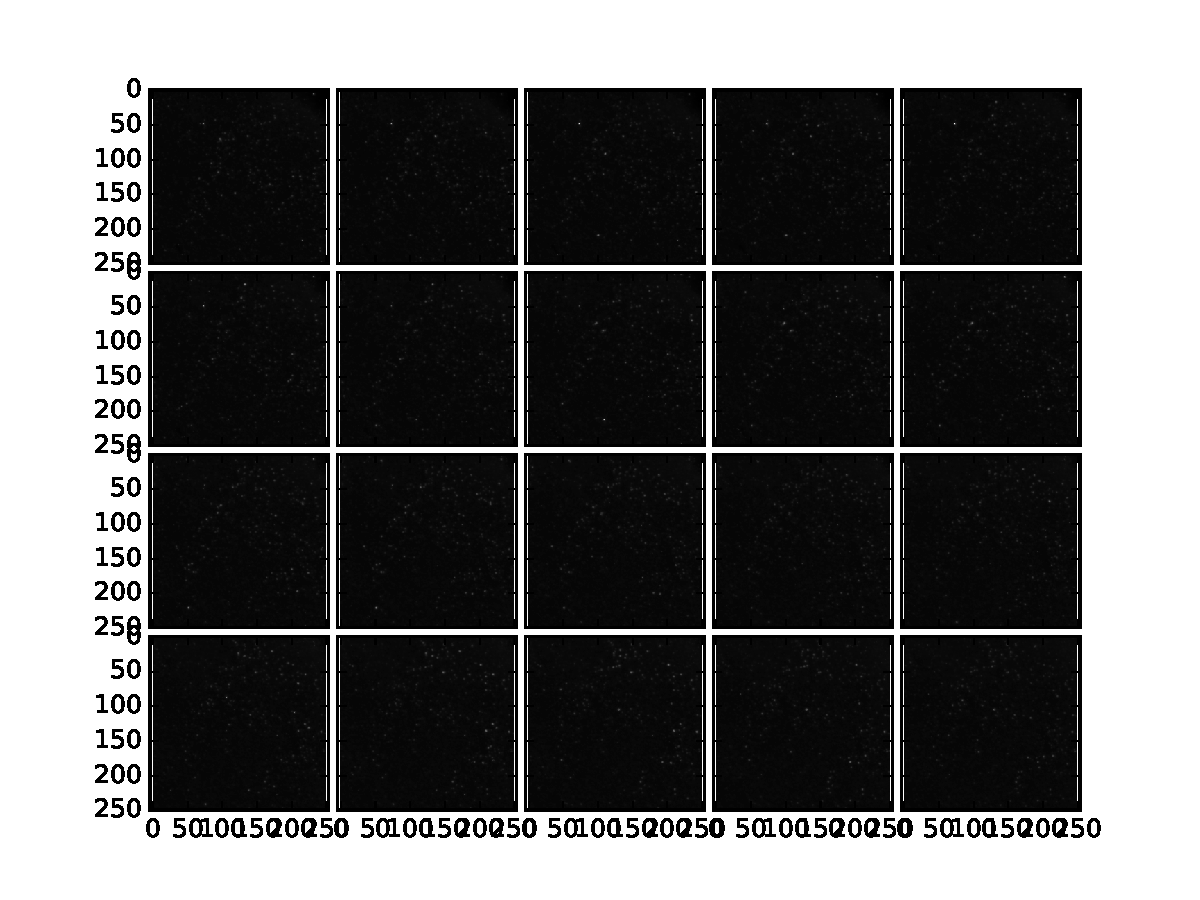
\includegraphics{imageanalysis-1.pdf}

To only plot a particular subregion its possible to specify the x,y,z range.

\begin{Verbatim}[commandchars=\\\{\}]
\PYG{g+gp}{\PYGZgt{}\PYGZgt{}\PYGZgt{} }\PYG{n}{plt}\PYG{o}{.}\PYG{n}{plotTiling}\PYG{p}{(}\PYG{n}{data}\PYG{p}{,} \PYG{n}{x} \PYG{o}{=} \PYG{p}{(}\PYG{l+m+mi}{0}\PYG{p}{,}\PYG{l+m+mi}{70}\PYG{p}{)}\PYG{p}{,} \PYG{n}{y} \PYG{o}{=} \PYG{p}{(}\PYG{l+m+mi}{0}\PYG{p}{,}\PYG{l+m+mi}{50}\PYG{p}{)}\PYG{p}{,} \PYG{n}{z} \PYG{o}{=} \PYG{p}{(}\PYG{l+m+mi}{10}\PYG{p}{,}\PYG{l+m+mi}{16}\PYG{p}{)}\PYG{p}{)}\PYG{p}{;}
\end{Verbatim}

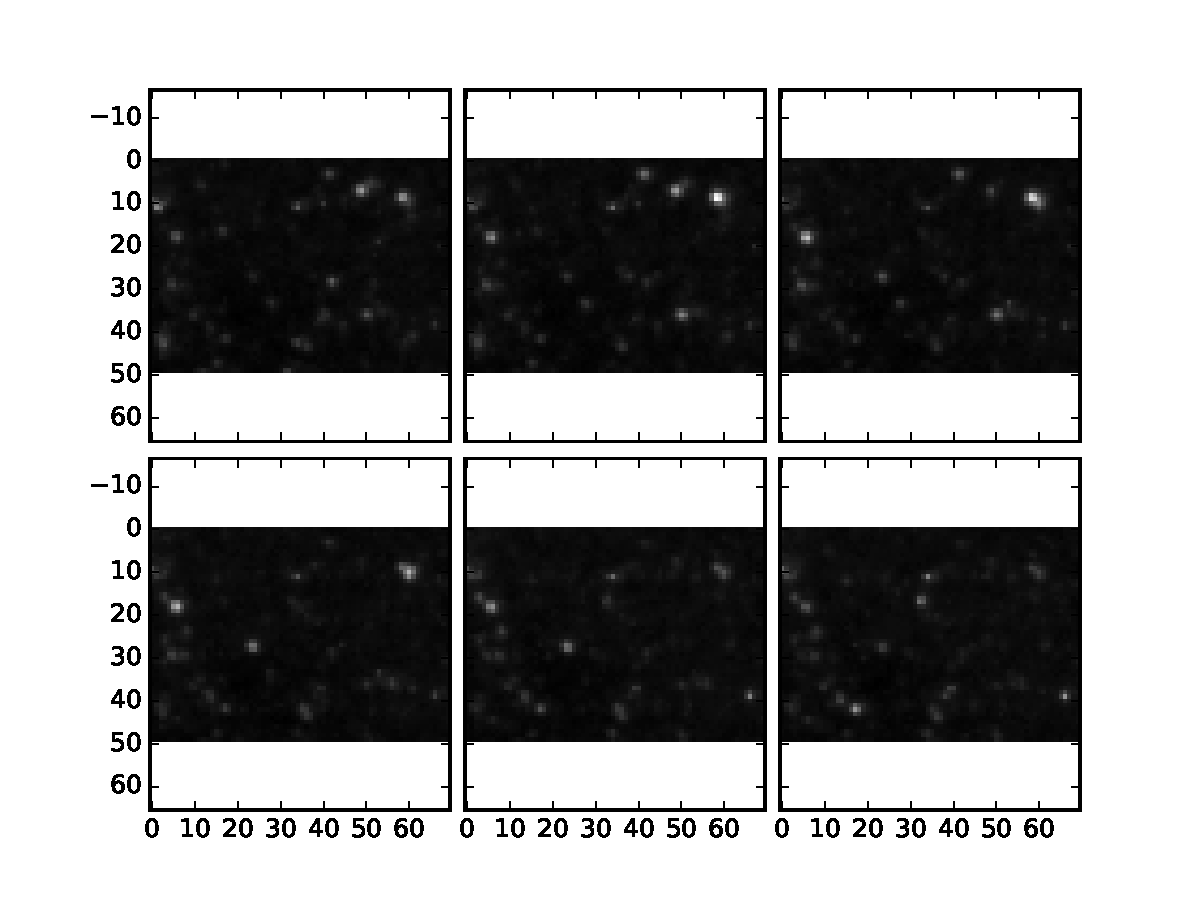
\includegraphics{imageanalysis-2.pdf}

Sometimes inverse colors may be better:

\begin{Verbatim}[commandchars=\\\{\}]
\PYG{g+gp}{\PYGZgt{}\PYGZgt{}\PYGZgt{} }\PYG{n}{plt}\PYG{o}{.}\PYG{n}{plotTiling}\PYG{p}{(}\PYG{n}{data}\PYG{p}{,} \PYG{n}{inverse} \PYG{o}{=} \PYG{n+nb+bp}{True}\PYG{p}{,}  \PYG{n}{z} \PYG{o}{=} \PYG{p}{(}\PYG{l+m+mi}{10}\PYG{p}{,}\PYG{l+m+mi}{16}\PYG{p}{)}\PYG{p}{)}\PYG{p}{;}
\end{Verbatim}

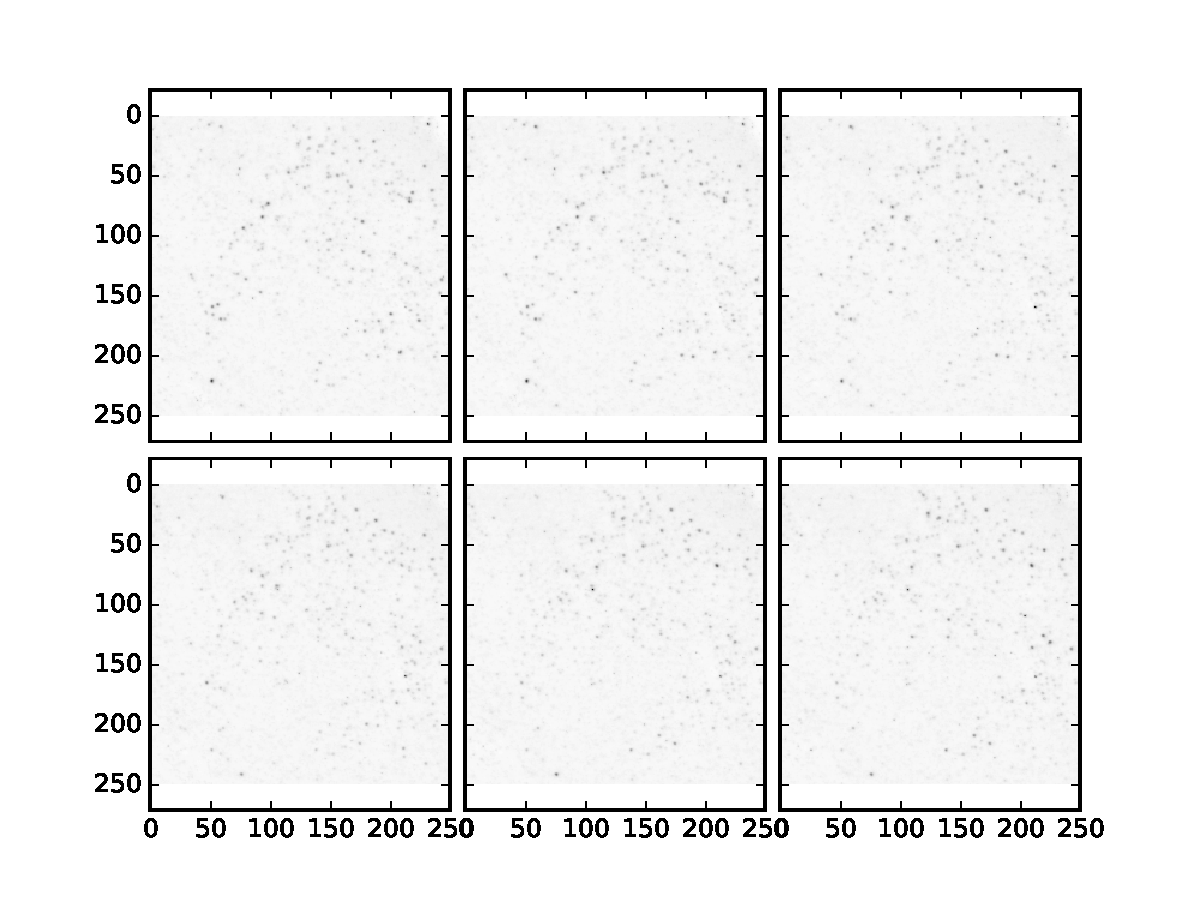
\includegraphics{imageanalysis-3.pdf}


\subsection{Image Statistics}
\label{imageanalysis:image-statistics}
It is useful to gather some information about the image initially.
For larger images that don’t fit in memory in ClearMap
certain statistics can be gathered in parallel via the
module {\hyperref[api/ClearMap.ImageProcessing:module-ClearMap.ImageProcessing.ImageStatistics]{\emph{\code{ClearMap.ImageProcessing.ImageStatistics}}}} module.

\begin{Verbatim}[commandchars=\\\{\}]
\PYG{g+gp}{\PYGZgt{}\PYGZgt{}\PYGZgt{} }\PYG{k+kn}{import} \PYG{n+nn}{ClearMap.ImageProcessing.ImageStatistics} \PYG{k+kn}{as} \PYG{n+nn}{stat}
\PYG{g+gp}{\PYGZgt{}\PYGZgt{}\PYGZgt{} }\PYG{k}{print} \PYG{n}{stat}\PYG{o}{.}\PYG{n}{calculateStatistics}\PYG{p}{(}\PYG{n}{filename}\PYG{p}{,} \PYG{n}{method} \PYG{o}{=} \PYG{l+s}{\PYGZsq{}}\PYG{l+s}{mean}\PYG{l+s}{\PYGZsq{}}\PYG{p}{)}
\PYG{g+go}{2305.4042155294119}
\end{Verbatim}

To get more information about the progress use the \code{verbose} option

\begin{Verbatim}[commandchars=\\\{\}]
\PYG{g+gp}{\PYGZgt{}\PYGZgt{}\PYGZgt{} }\PYG{k}{print} \PYG{n}{stat}\PYG{o}{.}\PYG{n}{calculateStatistics}\PYG{p}{(}\PYG{n}{filename}\PYG{p}{,} \PYG{n}{method} \PYG{o}{=} \PYG{l+s}{\PYGZsq{}}\PYG{l+s}{mean}\PYG{l+s}{\PYGZsq{}}\PYG{p}{,} \PYG{n}{verbose} \PYG{o}{=} \PYG{n+nb+bp}{True}\PYG{p}{)}
\PYG{g+go}{ChunkSize: Estimated chunk size 51 in 1 chunks!}
\PYG{g+go}{Number of SubStacks: 1}
\PYG{g+go}{Process 0: processing substack 0/1}
\PYG{g+go}{Process 0: file          = /ClearMap/Test/Data/ImageAnalysis/cfos\PYGZhy{}substack.tif}
\PYG{g+go}{Process 0: segmentation  = \PYGZlt{}function calculateStatisticsOnStack at 0x7fee9c25dd70\PYGZgt{}}
\PYG{g+go}{Process 0: ranges: x,y,z = \PYGZlt{}built\PYGZhy{}in function all\PYGZgt{},\PYGZlt{}built\PYGZhy{}in function all\PYGZgt{},(0, 51)}
\PYG{g+go}{Process 0: Reading data of size (250, 250, 51): elapsed time: 0:00:00}
\PYG{g+go}{Process 0: Processing substack of size (250, 250, 51): elapsed time: 0:00:00}
\PYG{g+go}{Total Time Image Statistics: elapsed time: 0:00:00}
\PYG{g+go}{2305.4042155294119}
\end{Verbatim}

Image statistics can be very helpful for modules, such as Ilastik, requiring a different bit depth than the original 16 or 12 bits files, as it helps to determine how to resample the images to a lower bit depth.


\subsection{Background Removal}
\label{imageanalysis:background-removal}
One of the first steps is often to remove background variations. The
\code{ClearMap.Imageprocessing.BackgroundRemoval} module can be used. It performs the background subtraction by morphological opening. The parameter is set as (x,y) where x and y are the diameter of an ellipsoid of a size close to the typical object detected in pixels. The intensity of the signal is greatly reduced after the filtering, but the signal-to-noise ration is increased:

\begin{Verbatim}[commandchars=\\\{\}]
\PYG{g+gp}{\PYGZgt{}\PYGZgt{}\PYGZgt{} }\PYG{k+kn}{import} \PYG{n+nn}{ClearMap.ImageProcessing.BackgroundRemoval} \PYG{k+kn}{as} \PYG{n+nn}{bgr}
\PYG{g+gp}{\PYGZgt{}\PYGZgt{}\PYGZgt{} }\PYG{n}{dataBGR} \PYG{o}{=} \PYG{n}{bgr}\PYG{o}{.}\PYG{n}{removeBackground}\PYG{p}{(}\PYG{n}{data}\PYG{o}{.}\PYG{n}{asype}\PYG{p}{(}\PYG{l+s}{\PYGZsq{}}\PYG{l+s}{float}\PYG{l+s}{\PYGZsq{}}\PYG{p}{)}\PYG{p}{,} \PYG{n}{size}\PYG{o}{=}\PYG{p}{(}\PYG{l+m+mi}{5}\PYG{p}{,}\PYG{l+m+mi}{5}\PYG{p}{)}\PYG{p}{,} \PYG{n}{verbose} \PYG{o}{=} \PYG{n+nb+bp}{True}\PYG{p}{)}\PYG{p}{;}
\PYG{g+gp}{\PYGZgt{}\PYGZgt{}\PYGZgt{} }\PYG{n}{plt}\PYG{o}{.}\PYG{n}{plotTiling}\PYG{p}{(}\PYG{n}{dataBGR}\PYG{p}{,} \PYG{n}{inverse} \PYG{o}{=} \PYG{n+nb+bp}{True}\PYG{p}{,} \PYG{n}{z} \PYG{o}{=} \PYG{p}{(}\PYG{l+m+mi}{10}\PYG{p}{,}\PYG{l+m+mi}{16}\PYG{p}{)}\PYG{p}{)}\PYG{p}{;}
\end{Verbatim}

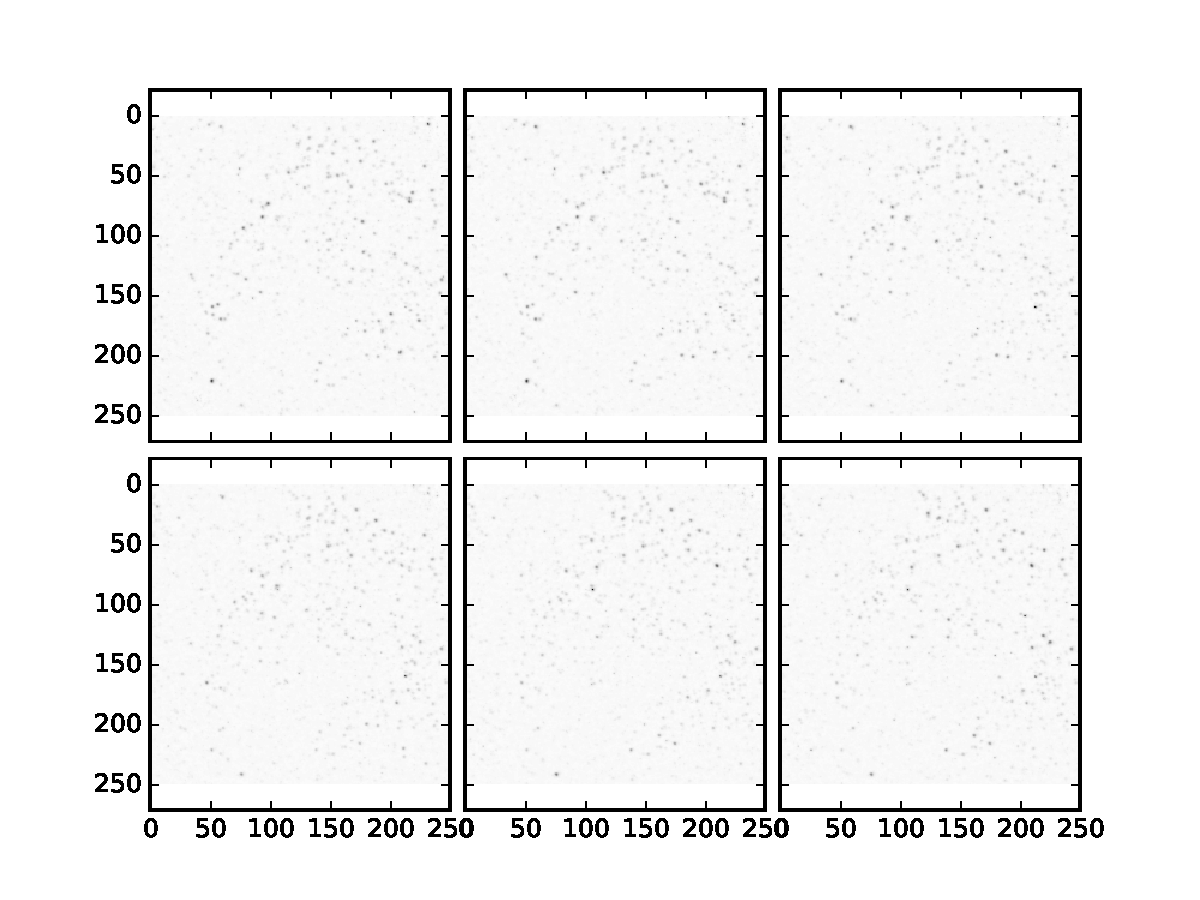
\includegraphics{imageanalysis-4.pdf}

Note that if the background feature size is chosen too small, this may result in removal of cells:

\begin{Verbatim}[commandchars=\\\{\}]
\PYG{g+gp}{\PYGZgt{}\PYGZgt{}\PYGZgt{} }\PYG{n}{dataBGR} \PYG{o}{=} \PYG{n}{bgr}\PYG{o}{.}\PYG{n}{removeBackground}\PYG{p}{(}\PYG{n}{data}\PYG{o}{.}\PYG{n}{astype}\PYG{p}{(}\PYG{l+s}{\PYGZsq{}}\PYG{l+s}{float}\PYG{l+s}{\PYGZsq{}}\PYG{p}{)}\PYG{p}{,} \PYG{n}{size}\PYG{o}{=}\PYG{p}{(}\PYG{l+m+mi}{3}\PYG{p}{,}\PYG{l+m+mi}{3}\PYG{p}{)}\PYG{p}{,} \PYG{n}{verbose} \PYG{o}{=} \PYG{n+nb+bp}{True}\PYG{p}{)}\PYG{p}{;}
\PYG{g+gp}{\PYGZgt{}\PYGZgt{}\PYGZgt{} }\PYG{n}{plt}\PYG{o}{.}\PYG{n}{plotTiling}\PYG{p}{(}\PYG{n}{dataBGR}\PYG{p}{,} \PYG{n}{inverse} \PYG{o}{=} \PYG{n+nb+bp}{True}\PYG{p}{,} \PYG{n}{z} \PYG{o}{=} \PYG{p}{(}\PYG{l+m+mi}{10}\PYG{p}{,}\PYG{l+m+mi}{16}\PYG{p}{)}\PYG{p}{)}\PYG{p}{;}
\end{Verbatim}

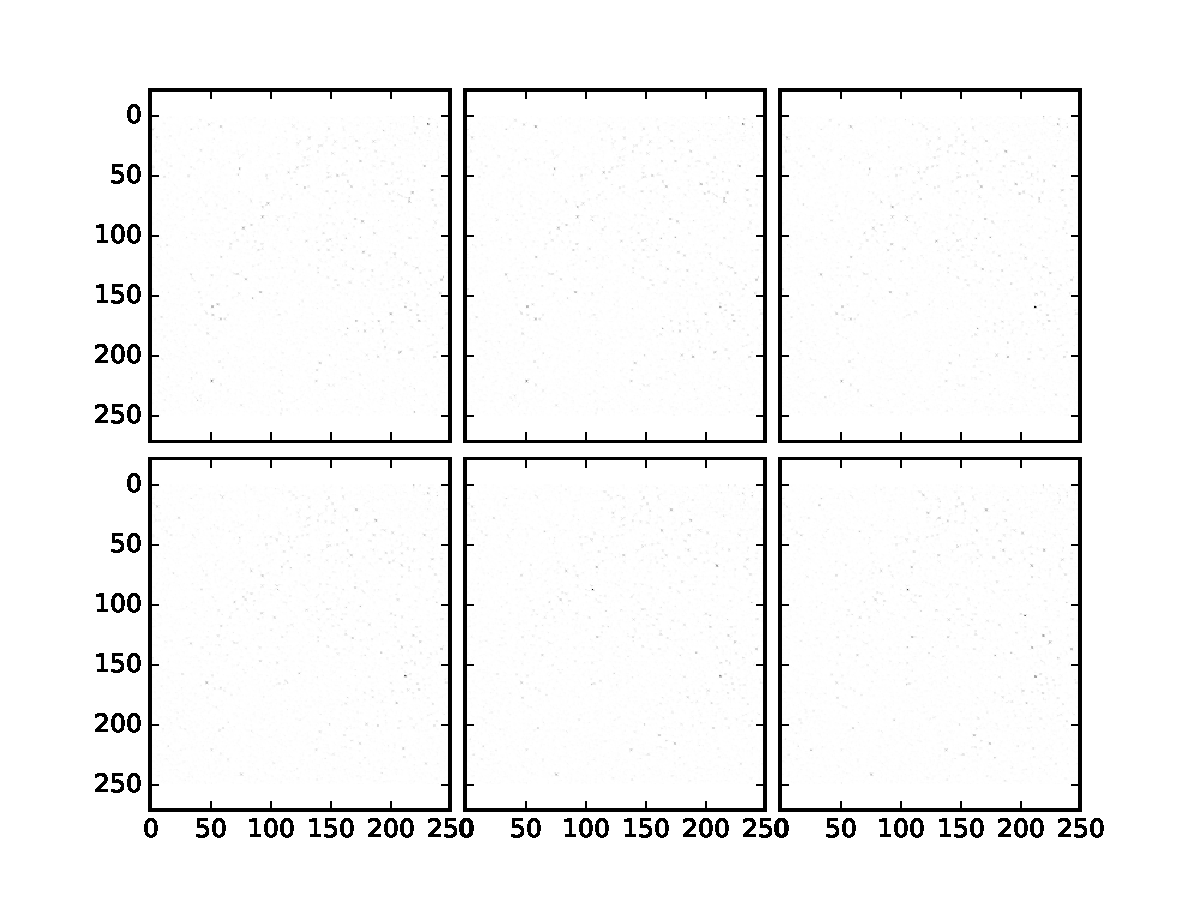
\includegraphics{imageanalysis-5.pdf}


\subsection{Image Filter}
\label{imageanalysis:image-filter}
A useful feature is to filter an image. Here the
\code{ClearMap.Imageprocessing.Filter} package can be used.

To detect cells center, the difference of Gaussians filter is a powerful way to increase the contrast between the cells and the background. The size is set as (x,y,z), and usually x, y and z are about the typical size in pixels of the detected object. As after the background subtraction, the intensity of the signal is again reduced after the filtering, but the signal-to-noise ration is dramatically increased:

\begin{Verbatim}[commandchars=\\\{\}]
\PYG{g+gp}{\PYGZgt{}\PYGZgt{}\PYGZgt{} }\PYG{k+kn}{from} \PYG{n+nn}{ClearMap.ImageProcessing.Filter.DoGFilter} \PYG{k+kn}{import} \PYG{n}{filterDoG}
\PYG{g+gp}{\PYGZgt{}\PYGZgt{}\PYGZgt{} }\PYG{n}{dataDoG} \PYG{o}{=} \PYG{n}{filterDoG}\PYG{p}{(}\PYG{n}{dataBGR}\PYG{p}{,} \PYG{n}{size}\PYG{o}{=}\PYG{p}{(}\PYG{l+m+mi}{8}\PYG{p}{,}\PYG{l+m+mi}{8}\PYG{p}{,}\PYG{l+m+mi}{4}\PYG{p}{)}\PYG{p}{,} \PYG{n}{verbose} \PYG{o}{=} \PYG{n+nb+bp}{True}\PYG{p}{)}\PYG{p}{;}
\PYG{g+gp}{\PYGZgt{}\PYGZgt{}\PYGZgt{} }\PYG{n}{plt}\PYG{o}{.}\PYG{n}{plotTiling}\PYG{p}{(}\PYG{n}{dataDoG}\PYG{p}{,} \PYG{n}{inverse} \PYG{o}{=} \PYG{n+nb+bp}{True}\PYG{p}{,} \PYG{n}{z} \PYG{o}{=} \PYG{p}{(}\PYG{l+m+mi}{10}\PYG{p}{,}\PYG{l+m+mi}{16}\PYG{p}{)}\PYG{p}{)}\PYG{p}{;}
\end{Verbatim}

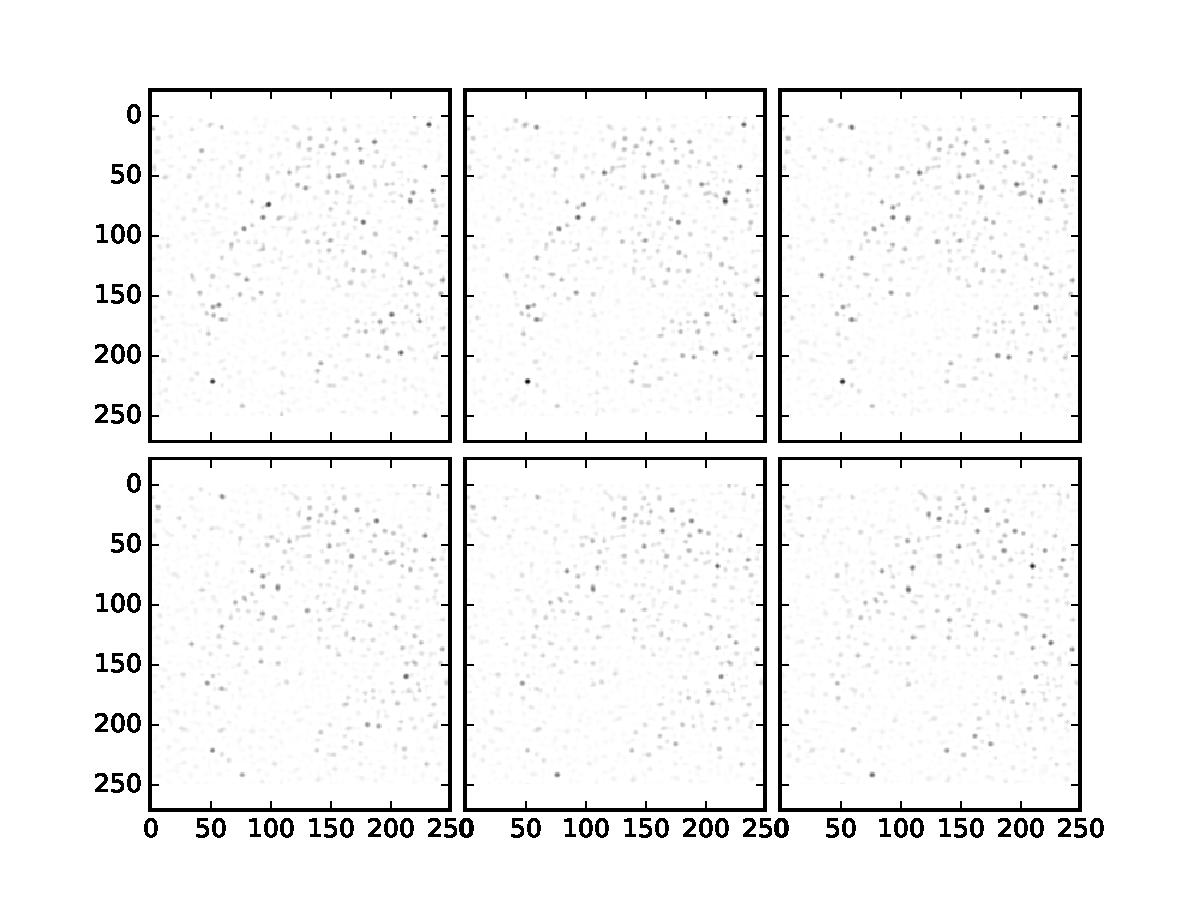
\includegraphics{imageanalysis-6.pdf}


\subsection{Maxima Detection}
\label{imageanalysis:maxima-detection}
The {\hyperref[api/ClearMap.ImageProcessing:module-ClearMap.ImageProcessing.MaximaDetection]{\emph{\code{ClearMap.ImageProcessing.MaximaDetection}}}} module contains a set
of useful functions for the detection of local maxima.
A labeled image can be visualized using the
{\hyperref[api/ClearMap.Visualization:ClearMap.Visualization.Plot.plotOverlayLabel]{\emph{\code{ClearMap.Visualization.Plot.plotOverlayLabel()}}}} routine.

\begin{Verbatim}[commandchars=\\\{\}]
\PYG{g+gp}{\PYGZgt{}\PYGZgt{}\PYGZgt{} }\PYG{k+kn}{from} \PYG{n+nn}{ClearMap.ImageProcessing.MaximaDetection} \PYG{k+kn}{import} \PYG{n}{findExtendedMaxima}
\PYG{g+gp}{\PYGZgt{}\PYGZgt{}\PYGZgt{} }\PYG{n}{dataMax} \PYG{o}{=} \PYG{n}{findExtendedMaxima}\PYG{p}{(}\PYG{n}{dataDoG}\PYG{p}{,} \PYG{n}{hMax} \PYG{o}{=} \PYG{n+nb+bp}{None}\PYG{p}{,} \PYG{n}{verbose} \PYG{o}{=} \PYG{n+nb+bp}{True}\PYG{p}{,} \PYG{n}{threshold} \PYG{o}{=} \PYG{l+m+mi}{10}\PYG{p}{)}\PYG{p}{;}
\PYG{g+gp}{\PYGZgt{}\PYGZgt{}\PYGZgt{} }\PYG{n}{plt}\PYG{o}{.}\PYG{n}{plotOverlayLabel}\PYG{p}{(}  \PYG{n}{dataDoG} \PYG{o}{/} \PYG{n}{dataDoG}\PYG{o}{.}\PYG{n}{max}\PYG{p}{(}\PYG{p}{)}\PYG{p}{,} \PYG{n}{dataMax}\PYG{o}{.}\PYG{n}{astype}\PYG{p}{(}\PYG{l+s}{\PYGZsq{}}\PYG{l+s}{int}\PYG{l+s}{\PYGZsq{}}\PYG{p}{)}\PYG{p}{,} \PYG{n}{z} \PYG{o}{=} \PYG{p}{(}\PYG{l+m+mi}{10}\PYG{p}{,}\PYG{l+m+mi}{16}\PYG{p}{)}\PYG{p}{)}
\end{Verbatim}

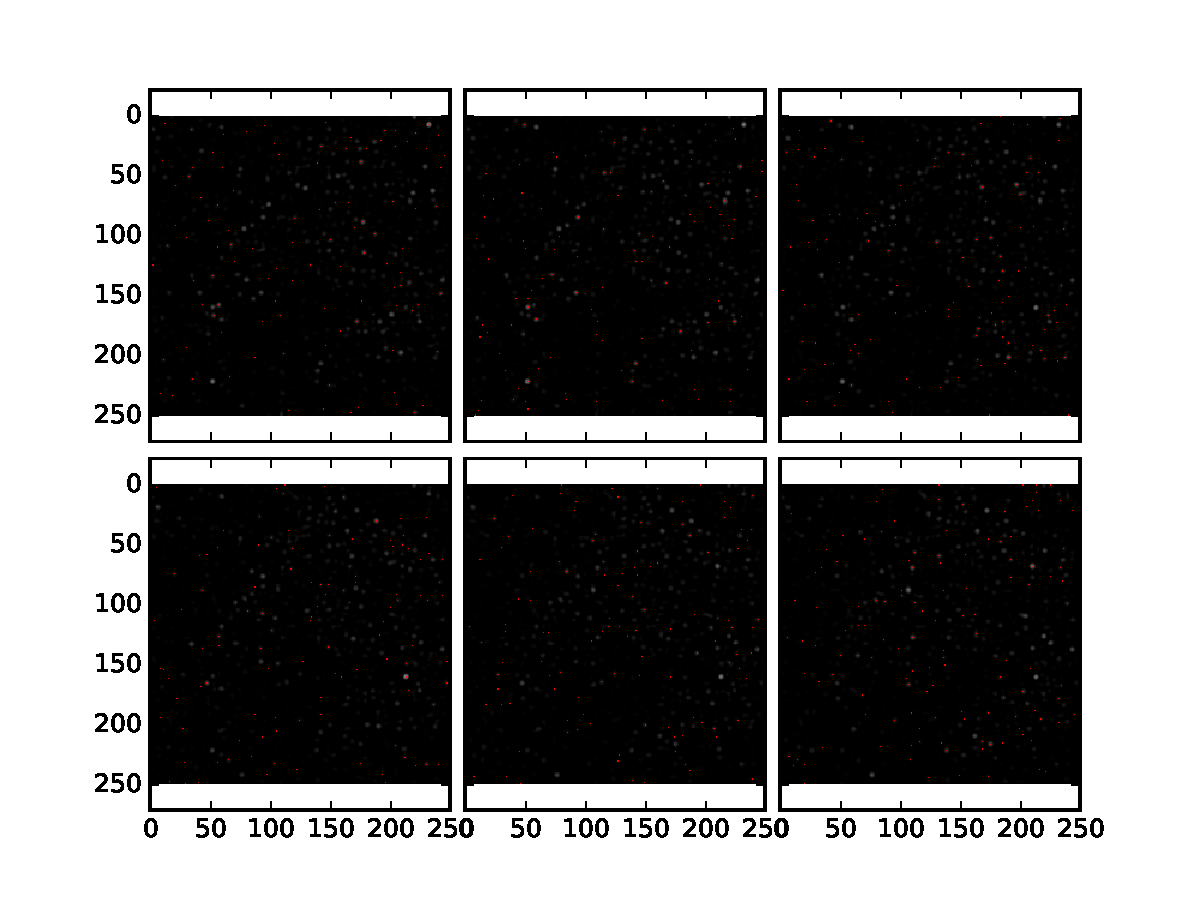
\includegraphics{imageanalysis-7.pdf}

Its easier to see when zoomed in:

\begin{Verbatim}[commandchars=\\\{\}]
\PYG{g+gp}{\PYGZgt{}\PYGZgt{}\PYGZgt{} }\PYG{n}{plt}\PYG{o}{.}\PYG{n}{plotOverlayLabel}\PYG{p}{(}\PYG{n}{dataDoG} \PYG{o}{/} \PYG{n}{dataDoG}\PYG{o}{.}\PYG{n}{max}\PYG{p}{(}\PYG{p}{)}\PYG{p}{,} \PYG{n}{dataMax}\PYG{o}{.}\PYG{n}{astype}\PYG{p}{(}\PYG{l+s}{\PYGZsq{}}\PYG{l+s}{int}\PYG{l+s}{\PYGZsq{}}\PYG{p}{)}\PYG{p}{,} \PYGZbs{}
\PYG{g+gp}{\PYGZgt{}\PYGZgt{}\PYGZgt{} }                     \PYG{n}{z} \PYG{o}{=} \PYG{p}{(}\PYG{l+m+mi}{10}\PYG{p}{,}\PYG{l+m+mi}{16}\PYG{p}{)}\PYG{p}{,} \PYG{n}{x} \PYG{o}{=} \PYG{p}{(}\PYG{l+m+mi}{50}\PYG{p}{,}\PYG{l+m+mi}{100}\PYG{p}{)}\PYG{p}{,}\PYG{n}{y} \PYG{o}{=} \PYG{p}{(}\PYG{l+m+mi}{50}\PYG{p}{,}\PYG{l+m+mi}{100}\PYG{p}{)}\PYG{p}{)}
\end{Verbatim}

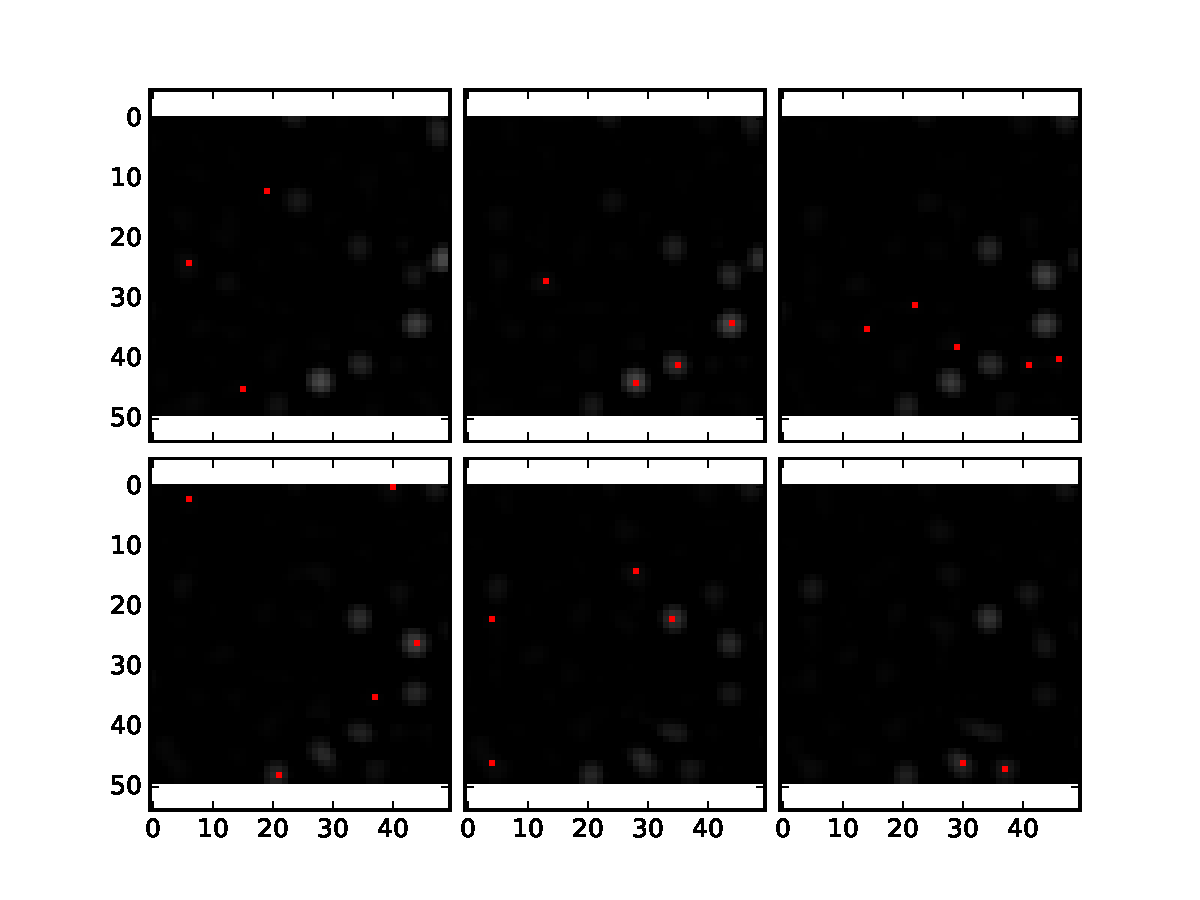
\includegraphics{imageanalysis-8.pdf}

Note that for some cells, a maxima label in this subset might not be visible as
maxima are detected in the entire image in 3D and the actual maxima
might lie in layers not shown above or below the current planes.

Once the maxima are detected the cell coordinates can be determined:

\begin{Verbatim}[commandchars=\\\{\}]
\PYG{g+gp}{\PYGZgt{}\PYGZgt{}\PYGZgt{} }\PYG{k+kn}{from} \PYG{n+nn}{ClearMap.ImageProcessing.MaximaDetection} \PYG{k+kn}{import} \PYG{n}{findCenterOfMaxima}
\PYG{g+gp}{\PYGZgt{}\PYGZgt{}\PYGZgt{} }\PYG{n}{cells} \PYG{o}{=} \PYG{n}{findCenterOfMaxima}\PYG{p}{(}\PYG{n}{data}\PYG{p}{,} \PYG{n}{dataMax}\PYG{p}{)}\PYG{p}{;}
\PYG{g+gp}{\PYGZgt{}\PYGZgt{}\PYGZgt{} }\PYG{k}{print} \PYG{n}{cells}\PYG{o}{.}\PYG{n}{shape}
\PYG{g+go}{(3670, 3)}
\end{Verbatim}

We can also overlay the cell coordinates in an image:

\begin{Verbatim}[commandchars=\\\{\}]
\PYG{g+gp}{\PYGZgt{}\PYGZgt{}\PYGZgt{} }\PYG{n}{plt}\PYG{o}{.}\PYG{n}{plotOverlayPoints}\PYG{p}{(}\PYG{n}{data}\PYG{p}{,} \PYG{n}{cells}\PYG{p}{,} \PYG{n}{z} \PYG{o}{=} \PYG{p}{(}\PYG{l+m+mi}{10}\PYG{p}{,}\PYG{l+m+mi}{16}\PYG{p}{)}\PYG{p}{)}
\end{Verbatim}

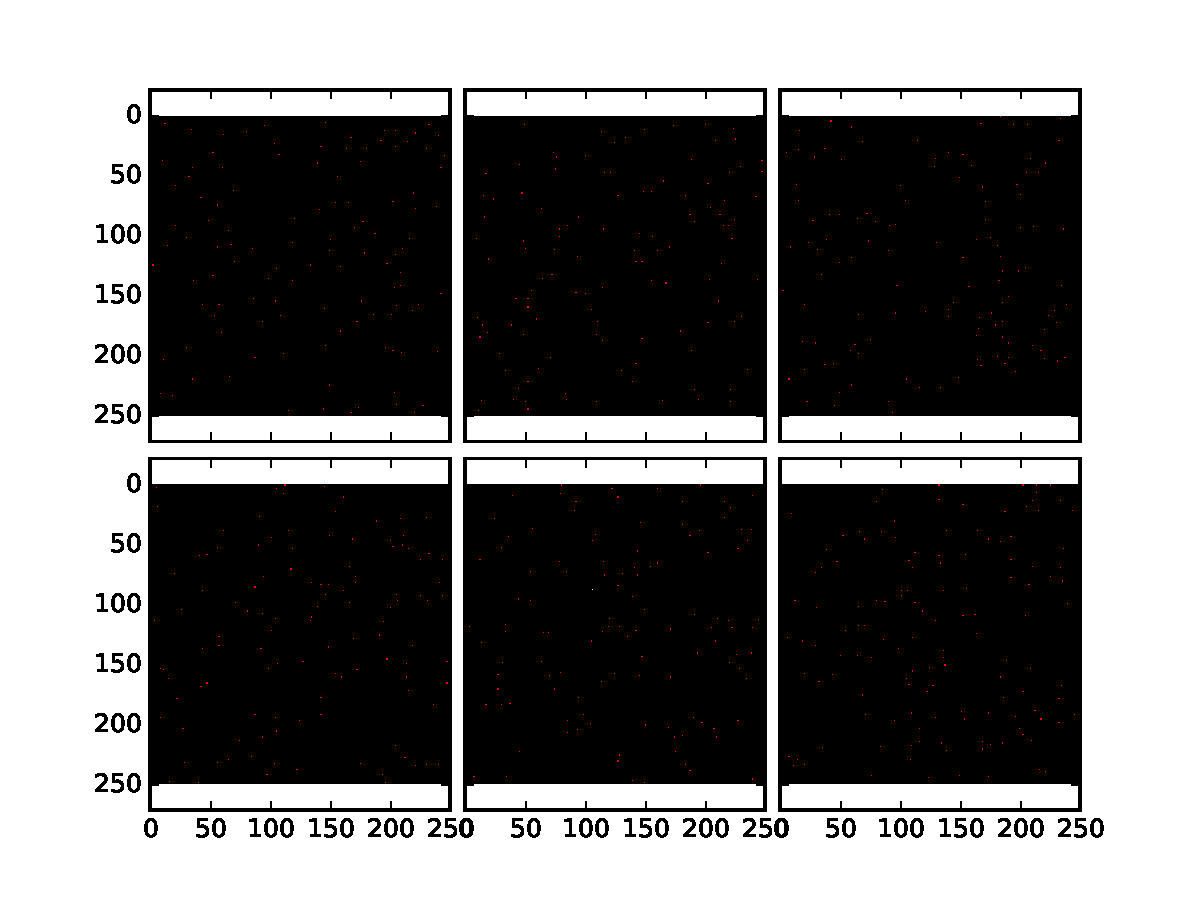
\includegraphics{imageanalysis-9.pdf}


\subsection{Cell Shape Detection}
\label{imageanalysis:cell-shape-detection}
Finally once the cell centers are detected the
\code{ClearMap.ImageProcessing.CellShapedetection} module can be used to detect
the cell shape via a watershed.

\begin{Verbatim}[commandchars=\\\{\}]
\PYG{g+gp}{\PYGZgt{}\PYGZgt{}\PYGZgt{} }\PYG{k+kn}{from} \PYG{n+nn}{ClearMap.ImageProcessing.CellSizeDetection} \PYG{k+kn}{import} \PYG{n}{detectCellShape}
\PYG{g+gp}{\PYGZgt{}\PYGZgt{}\PYGZgt{} }\PYG{n}{dataShape} \PYG{o}{=} \PYG{n}{detectCellShape}\PYG{p}{(}\PYG{n}{dataDoG}\PYG{p}{,} \PYG{n}{cells}\PYG{p}{,} \PYG{n}{threshold} \PYG{o}{=} \PYG{l+m+mi}{15}\PYG{p}{)}\PYG{p}{;}
\PYG{g+gp}{\PYGZgt{}\PYGZgt{}\PYGZgt{} }\PYG{n}{plt}\PYG{o}{.}\PYG{n}{plotOverlayLabel}\PYG{p}{(}\PYG{n}{dataDoG} \PYG{o}{/} \PYG{n}{dataDoG}\PYG{o}{.}\PYG{n}{max}\PYG{p}{(}\PYG{p}{)}\PYG{p}{,} \PYG{n}{dataShape}\PYG{p}{,} \PYG{n}{z} \PYG{o}{=} \PYG{p}{(}\PYG{l+m+mi}{10}\PYG{p}{,}\PYG{l+m+mi}{16}\PYG{p}{)}\PYG{p}{)}
\end{Verbatim}

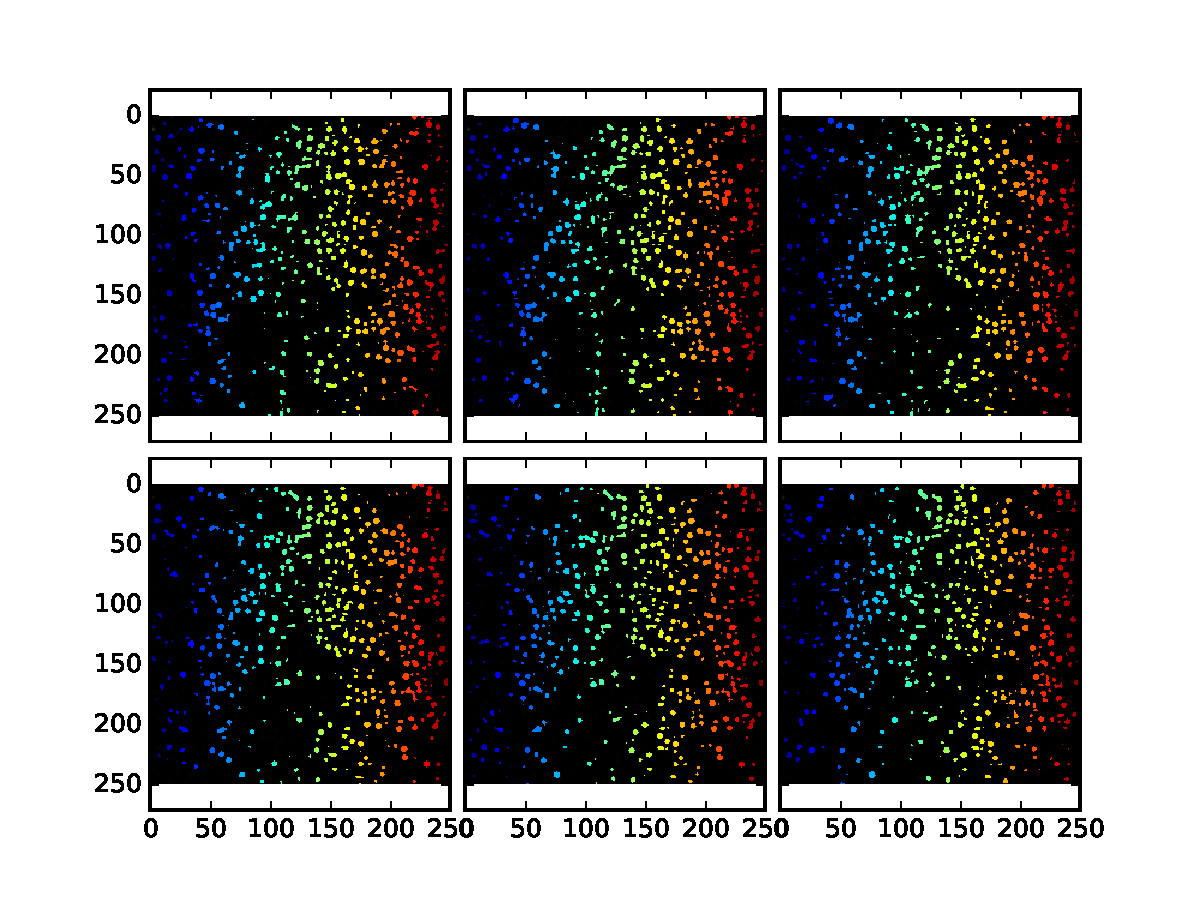
\includegraphics{imageanalysis-10.pdf}

Now we can perform some measurements:

\begin{Verbatim}[commandchars=\\\{\}]
\PYG{g+gp}{\PYGZgt{}\PYGZgt{}\PYGZgt{} }\PYG{k+kn}{from} \PYG{n+nn}{ClearMap.ImageProcessing.CellSizeDetection} \PYG{k+kn}{import} \PYG{n}{findCellSize}\PYG{p}{,}\PYGZbs{}
\PYG{g+gp}{\PYGZgt{}\PYGZgt{}\PYGZgt{} }                                                       \PYG{n}{findCellIntensity}
\PYG{g+gp}{\PYGZgt{}\PYGZgt{}\PYGZgt{} }\PYG{n}{cellSizes} \PYG{o}{=} \PYG{n}{findCellSize}\PYG{p}{(}\PYG{n}{dataShape}\PYG{p}{,} \PYG{n}{maxLabel} \PYG{o}{=} \PYG{n}{cells}\PYG{o}{.}\PYG{n}{shape}\PYG{p}{[}\PYG{l+m+mi}{0}\PYG{p}{]}\PYG{p}{)}\PYG{p}{;}
\PYG{g+gp}{\PYGZgt{}\PYGZgt{}\PYGZgt{} }\PYG{n}{cellIntensities} \PYG{o}{=} \PYG{n}{findCellIntensity}\PYG{p}{(}\PYG{n}{dataBGR}\PYG{p}{,} \PYG{n}{dataShape}\PYG{p}{,} \PYG{n}{maxLabel} \PYG{o}{=} \PYG{n}{cells}\PYG{o}{.}\PYG{n}{shape}\PYG{p}{[}\PYG{l+m+mi}{0}\PYG{p}{]}\PYG{p}{)}\PYG{p}{;}
\end{Verbatim}

and plot those:

\begin{Verbatim}[commandchars=\\\{\}]
\PYG{g+gp}{\PYGZgt{}\PYGZgt{}\PYGZgt{} }\PYG{k+kn}{import} \PYG{n+nn}{matplotlib.pyplot} \PYG{k+kn}{as} \PYG{n+nn}{mpl}
\PYG{g+gp}{\PYGZgt{}\PYGZgt{}\PYGZgt{} }\PYG{n}{mpl}\PYG{o}{.}\PYG{n}{figure}\PYG{p}{(}\PYG{p}{)}
\PYG{g+gp}{\PYGZgt{}\PYGZgt{}\PYGZgt{} }\PYG{n}{mpl}\PYG{o}{.}\PYG{n}{plot}\PYG{p}{(}\PYG{n}{cellSizes}\PYG{p}{,} \PYG{n}{cellIntensities}\PYG{p}{,} \PYG{l+s}{\PYGZsq{}}\PYG{l+s}{.}\PYG{l+s}{\PYGZsq{}}\PYG{p}{)}
\PYG{g+gp}{\PYGZgt{}\PYGZgt{}\PYGZgt{} }\PYG{n}{mpl}\PYG{o}{.}\PYG{n}{xlabel}\PYG{p}{(}\PYG{l+s}{\PYGZsq{}}\PYG{l+s}{cell size [voxel]}\PYG{l+s}{\PYGZsq{}}\PYG{p}{)}
\PYG{g+gp}{\PYGZgt{}\PYGZgt{}\PYGZgt{} }\PYG{n}{mpl}\PYG{o}{.}\PYG{n}{ylabel}\PYG{p}{(}\PYG{l+s}{\PYGZsq{}}\PYG{l+s}{cell intensity [au]}\PYG{l+s}{\PYGZsq{}}\PYG{p}{)}
\end{Verbatim}

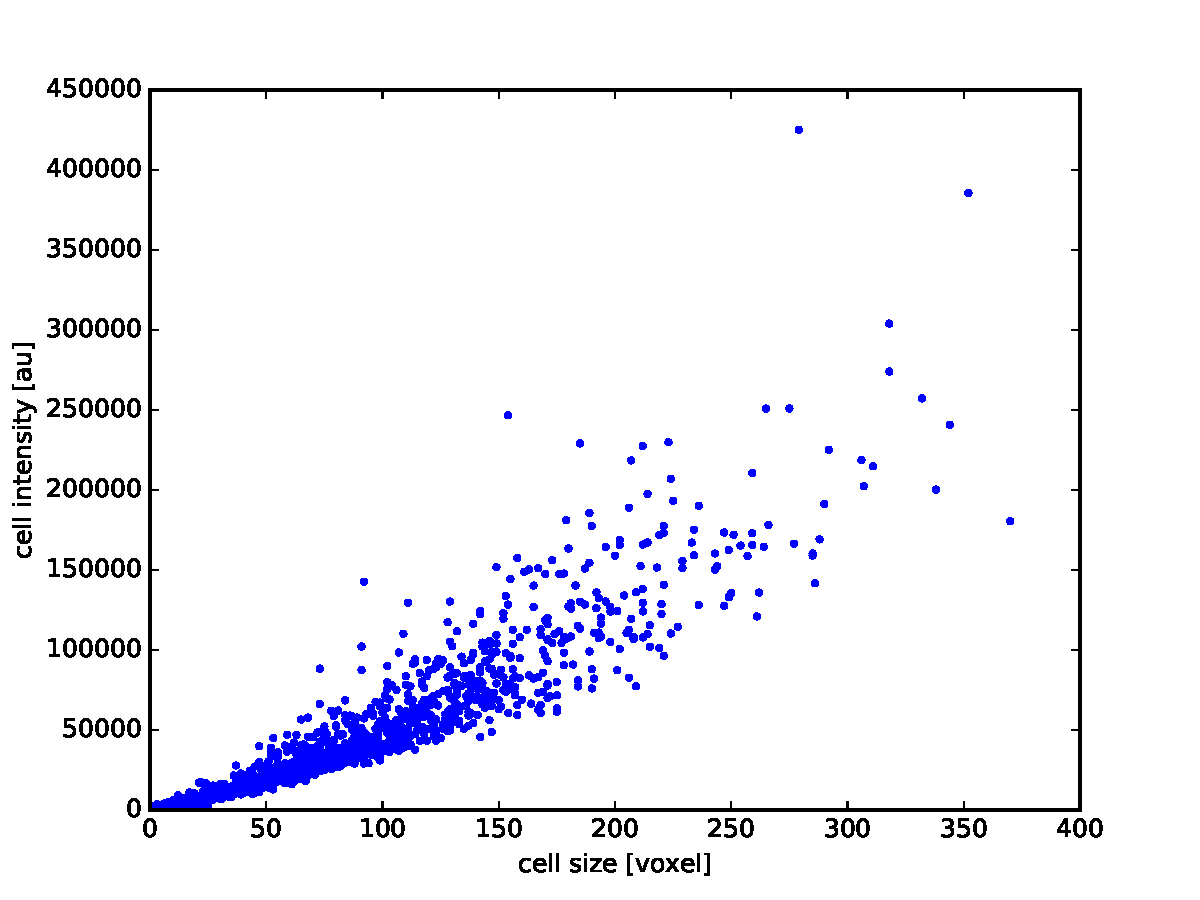
\includegraphics{imageanalysis-11.pdf}


\section{Roadmap}
\label{roadmap::doc}\label{roadmap:roadmap}
ClearMap is going to develop further to extend its functionality and useability.


\subsection{Plans for future developoment:}
\label{roadmap:plans-for-future-developoment}
We plan to add following items to ClearMap in the future:
\begin{itemize}
\item {} 
Graphical User Interface

\item {} 
Flexible pipeline generation

\item {} 
Colocalization tools

\item {} 
Tracing tools

\item {} 
Support for very large data sets and memmaps

\end{itemize}

Together with those changes some additional changes will be done to the code
under the hood:
\begin{itemize}
\item {} 
reorganization of the IO module

\item {} 
reorganization of the parameter specifications

\item {} 
reorganization of the parallel processing

\end{itemize}


\section{Issues}
\label{issues::doc}\label{issues:issues}
This is a list of know issues in Clearmap:
\begin{itemize}
\item {} 
for very large stiched images the watershed results shows a cutoff at large coordinates

\item {} 
for multipage tiff files the resampling method can get stuck, use sequential tiff stacks instead

\end{itemize}


\chapter{ClearMap functions}
\label{index:clearmap-functions}

\section{ClearMap package}
\label{api/ClearMap:clearmap-package}\label{api/ClearMap::doc}\phantomsection\label{api/ClearMap:module-ClearMap}\index{ClearMap (module)}
\emph{ClearMap} is a python toolbox for the analysis and registration of volumetric
data from cleared tissues obtained with Light Sheet microscopy.

The ClearMap code package is structured into four main modules:
\begin{itemize}
\item {} 
\textbf{IO} for reading and writing images and data

\item {} 
\textbf{Alignment} for resampling, reorientation and registration of images onto references

\item {} 
\textbf{Image Processing} for correcting and quantifying the image data

\item {} 
\textbf{Analysis} for the statistical analysis of the data

\end{itemize}


\subsection{Subpackages}
\label{api/ClearMap:subpackages}

\subsubsection{ClearMap.IO package}
\label{api/ClearMap.IO:clearmap-io-package}\label{api/ClearMap.IO::doc}\label{api/ClearMap.IO:module-ClearMap.IO}\index{ClearMap.IO (module)}
This sub-package provides routines to read and write data
\begin{description}
\item[{Two types of data files are discriminated:}] \leavevmode\begin{itemize}
\item {} 
{\hyperref[api/ClearMap.IO:image-data]{\emph{Image data}}}

\item {} 
{\hyperref[api/ClearMap.IO:point-data]{\emph{Point data}}}

\end{itemize}

\end{description}

The image data are stacks from microscopes obtained by volume imaging, or the results of analysis representing
the visualization of the detected objects for instance.

The point data are lists of cell coordinates or measured intensities for instance.


\paragraph{Image data}
\label{api/ClearMap.IO:image-data}
Images are represented internally as numpy arrays. ClearMap assumes images
in arrays are arranged as {[}x,y{]}, {[}x,y,z{]} or {[}x,y,z,c{]} where x,y,z correspond to
the x,y,z coordinates as when viewed in an image viewer such as ImageJ.
The c coordinate is a possible color channel.

\begin{notice}{note}{Note:}
Many image libraries read images as {[}y,x,z{]} or {[}y,x{]} arrays!
\end{notice}

The ClearMap toolbox supports a range of (volumetric) image formats:

\begin{tabulary}{\linewidth}{|L|L|L|}
\hline
\textsf{\relax 
Format
} & \textsf{\relax 
Descrition
} & \textsf{\relax 
Module
}\\
\hline
TIF
 & 
tif images and stacks
 & 
{\hyperref[api/ClearMap.IO:module-ClearMap.IO.TIF]{\emph{\code{TIF}}}}
\\
\hline
RAW / MHD
 & 
raw image files with optional mhd header file
 & 
{\hyperref[api/ClearMap.IO:module-ClearMap.IO.RAW]{\emph{\code{RAW}}}}
\\
\hline
NRRD
 & 
nearly raw raster data files
 & 
{\hyperref[api/ClearMap.IO:module-ClearMap.IO.NRRD]{\emph{\code{NRRD}}}}
\\
\hline
IMS
 & 
imaris image file
 & 
{\hyperref[api/ClearMap.IO:module-ClearMap.IO.Imaris]{\emph{\code{Imaris}}}}
\\
\hline
reg exp
 & 
folder, file list or file pattern of a stack of 2d images
 & 
{\hyperref[api/ClearMap.IO:module-ClearMap.IO.FileList]{\emph{\code{FileList}}}}
\\
\hline\end{tabulary}


\begin{notice}{note}{Note:}
ClearMap can read the image data from a Bitplane’s Imaris, but can’t export image data as an Imaris file.
\end{notice}

The image format is inferred automatically from the file name extension.

For example to read image data use {\hyperref[api/ClearMap.IO:ClearMap.IO.IO.readData]{\emph{\code{readData()}}}}:

\begin{Verbatim}[commandchars=\\\{\}]
\PYG{g+gp}{\PYGZgt{}\PYGZgt{}\PYGZgt{} }\PYG{k+kn}{import} \PYG{n+nn}{os}
\PYG{g+gp}{\PYGZgt{}\PYGZgt{}\PYGZgt{} }\PYG{k+kn}{import} \PYG{n+nn}{ClearMap.IO} \PYG{k+kn}{as} \PYG{n+nn}{io}
\PYG{g+gp}{\PYGZgt{}\PYGZgt{}\PYGZgt{} }\PYG{k+kn}{import} \PYG{n+nn}{ClearMap.Settings} \PYG{k+kn}{as} \PYG{n+nn}{settings}
\PYG{g+gp}{\PYGZgt{}\PYGZgt{}\PYGZgt{} }\PYG{n}{filename} \PYG{o}{=} \PYG{n}{os}\PYG{o}{.}\PYG{n}{path}\PYG{o}{.}\PYG{n}{join}\PYG{p}{(}\PYG{n}{settings}\PYG{o}{.}\PYG{n}{ClearMapPath}\PYG{p}{,}\PYG{l+s}{\PYGZsq{}}\PYG{l+s}{Test/Data/Tif/test.tif}\PYG{l+s}{\PYGZsq{}}\PYG{p}{)}\PYG{p}{;}
\PYG{g+gp}{\PYGZgt{}\PYGZgt{}\PYGZgt{} }\PYG{n}{data} \PYG{o}{=} \PYG{n}{io}\PYG{o}{.}\PYG{n}{readData}\PYG{p}{(}\PYG{n}{filename}\PYG{p}{)}\PYG{p}{;}
\PYG{g+gp}{\PYGZgt{}\PYGZgt{}\PYGZgt{} }\PYG{k}{print} \PYG{n}{data}\PYG{o}{.}\PYG{n}{shape}
\PYG{g+go}{(20, 50, 10)}
\end{Verbatim}

To write image data use {\hyperref[api/ClearMap.IO:ClearMap.IO.IO.writeData]{\emph{\code{writeData()}}}}:

\begin{Verbatim}[commandchars=\\\{\}]
\PYG{g+gp}{\PYGZgt{}\PYGZgt{}\PYGZgt{} }\PYG{k+kn}{import} \PYG{n+nn}{os}\PYG{o}{,} \PYG{n+nn}{numpy}
\PYG{g+gp}{\PYGZgt{}\PYGZgt{}\PYGZgt{} }\PYG{k+kn}{import} \PYG{n+nn}{ClearMap.IO} \PYG{k+kn}{as} \PYG{n+nn}{io}
\PYG{g+gp}{\PYGZgt{}\PYGZgt{}\PYGZgt{} }\PYG{k+kn}{import} \PYG{n+nn}{ClearMap.Settings} \PYG{k+kn}{as} \PYG{n+nn}{settings}
\PYG{g+gp}{\PYGZgt{}\PYGZgt{}\PYGZgt{} }\PYG{n}{filename} \PYG{o}{=} \PYG{n}{os}\PYG{o}{.}\PYG{n}{path}\PYG{o}{.}\PYG{n}{join}\PYG{p}{(}\PYG{n}{settings}\PYG{o}{.}\PYG{n}{ClearMapPath}\PYG{p}{,}\PYG{l+s}{\PYGZsq{}}\PYG{l+s}{Test/Data/Tif/test.tif}\PYG{l+s}{\PYGZsq{}}\PYG{p}{)}\PYG{p}{;}
\PYG{g+gp}{\PYGZgt{}\PYGZgt{}\PYGZgt{} }\PYG{n}{data} \PYG{o}{=} \PYG{n}{numpy}\PYG{o}{.}\PYG{n}{random}\PYG{o}{.}\PYG{n}{rand}\PYG{p}{(}\PYG{l+m+mi}{20}\PYG{p}{,}\PYG{l+m+mi}{50}\PYG{p}{,}\PYG{l+m+mi}{10}\PYG{p}{)}\PYG{p}{;}
\PYG{g+gp}{\PYGZgt{}\PYGZgt{}\PYGZgt{} }\PYG{n}{data}\PYG{p}{[}\PYG{l+m+mi}{5}\PYG{p}{:}\PYG{l+m+mi}{15}\PYG{p}{,} \PYG{l+m+mi}{20}\PYG{p}{:}\PYG{l+m+mi}{45}\PYG{p}{,} \PYG{l+m+mi}{2}\PYG{p}{:}\PYG{l+m+mi}{9}\PYG{p}{]} \PYG{o}{=} \PYG{l+m+mi}{0}\PYG{p}{;}
\PYG{g+gp}{\PYGZgt{}\PYGZgt{}\PYGZgt{} }\PYG{n}{data} \PYG{o}{=} \PYG{l+m+mi}{20} \PYG{o}{*} \PYG{n}{data}\PYG{p}{;}
\PYG{g+gp}{\PYGZgt{}\PYGZgt{}\PYGZgt{} }\PYG{n}{data} \PYG{o}{=} \PYG{n}{data}\PYG{o}{.}\PYG{n}{astype}\PYG{p}{(}\PYG{l+s}{\PYGZsq{}}\PYG{l+s}{int32}\PYG{l+s}{\PYGZsq{}}\PYG{p}{)}\PYG{p}{;}
\PYG{g+gp}{\PYGZgt{}\PYGZgt{}\PYGZgt{} }\PYG{n}{res} \PYG{o}{=} \PYG{n}{io}\PYG{o}{.}\PYG{n}{writeData}\PYG{p}{(}\PYG{n}{filename}\PYG{p}{,} \PYG{n}{data}\PYG{p}{)}\PYG{p}{;}
\PYG{g+gp}{\PYGZgt{}\PYGZgt{}\PYGZgt{} }\PYG{k}{print} \PYG{n}{io}\PYG{o}{.}\PYG{n}{dataSize}\PYG{p}{(}\PYG{n}{res}\PYG{p}{)}\PYG{p}{;}
\PYG{g+go}{(20, 50, 10)}
\end{Verbatim}

Generally, the IO module is designed to work with image sources which can be
either files or already loaded numpy arrays. This is important to enable flexible
parallel processing, without rewriting the data analysis routines.

For example:

\begin{Verbatim}[commandchars=\\\{\}]
\PYG{g+gp}{\PYGZgt{}\PYGZgt{}\PYGZgt{} }\PYG{k+kn}{import} \PYG{n+nn}{numpy}
\PYG{g+gp}{\PYGZgt{}\PYGZgt{}\PYGZgt{} }\PYG{k+kn}{import} \PYG{n+nn}{ClearMap.IO} \PYG{k+kn}{as} \PYG{n+nn}{io}
\PYG{g+gp}{\PYGZgt{}\PYGZgt{}\PYGZgt{} }\PYG{n}{data} \PYG{o}{=} \PYG{n}{numpy}\PYG{o}{.}\PYG{n}{random}\PYG{o}{.}\PYG{n}{rand}\PYG{p}{(}\PYG{l+m+mi}{20}\PYG{p}{,}\PYG{l+m+mi}{50}\PYG{p}{,}\PYG{l+m+mi}{10}\PYG{p}{)}\PYG{p}{;}
\PYG{g+gp}{\PYGZgt{}\PYGZgt{}\PYGZgt{} }\PYG{n}{res} \PYG{o}{=} \PYG{n}{io}\PYG{o}{.}\PYG{n}{writeData}\PYG{p}{(}\PYG{n+nb+bp}{None}\PYG{p}{,} \PYG{n}{data}\PYG{p}{)}\PYG{p}{;}
\PYG{g+gp}{\PYGZgt{}\PYGZgt{}\PYGZgt{} }\PYG{k}{print} \PYG{n}{res}\PYG{o}{.}\PYG{n}{shape}\PYG{p}{;}
\PYG{g+go}{(20, 50, 10)}
\end{Verbatim}

Range parameter can be passed in order to only load sub sets of image data,
useful when the images are very large. For example to load a sub-image:

\begin{Verbatim}[commandchars=\\\{\}]
\PYG{g+gp}{\PYGZgt{}\PYGZgt{}\PYGZgt{} }\PYG{k+kn}{import} \PYG{n+nn}{os}\PYG{o}{,} \PYG{n+nn}{numpy}
\PYG{g+gp}{\PYGZgt{}\PYGZgt{}\PYGZgt{} }\PYG{k+kn}{import} \PYG{n+nn}{ClearMap.IO} \PYG{k+kn}{as} \PYG{n+nn}{io}
\PYG{g+gp}{\PYGZgt{}\PYGZgt{}\PYGZgt{} }\PYG{k+kn}{import} \PYG{n+nn}{ClearMap.Settings} \PYG{k+kn}{as} \PYG{n+nn}{settings}
\PYG{g+gp}{\PYGZgt{}\PYGZgt{}\PYGZgt{} }\PYG{n}{filename} \PYG{o}{=} \PYG{n}{os}\PYG{o}{.}\PYG{n}{path}\PYG{o}{.}\PYG{n}{join}\PYG{p}{(}\PYG{n}{settings}\PYG{o}{.}\PYG{n}{ClearMapPath}\PYG{p}{,}\PYG{l+s}{\PYGZsq{}}\PYG{l+s}{Test/Data/Tif/test.tif}\PYG{l+s}{\PYGZsq{}}\PYG{p}{)}\PYG{p}{;}
\PYG{g+gp}{\PYGZgt{}\PYGZgt{}\PYGZgt{} }\PYG{n}{res} \PYG{o}{=} \PYG{n}{io}\PYG{o}{.}\PYG{n}{readData}\PYG{p}{(}\PYG{n}{filename}\PYG{p}{,} \PYG{n}{data}\PYG{p}{,} \PYG{n}{x} \PYG{o}{=} \PYG{p}{(}\PYG{l+m+mi}{0}\PYG{p}{,}\PYG{l+m+mi}{3}\PYG{p}{)}\PYG{p}{,} \PYG{n}{y} \PYG{o}{=} \PYG{p}{(}\PYG{l+m+mi}{4}\PYG{p}{,}\PYG{l+m+mi}{6}\PYG{p}{)}\PYG{p}{,} \PYG{n}{z} \PYG{o}{=} \PYG{p}{(}\PYG{l+m+mi}{1}\PYG{p}{,}\PYG{l+m+mi}{4}\PYG{p}{)}\PYG{p}{)}\PYG{p}{;}
\PYG{g+gp}{\PYGZgt{}\PYGZgt{}\PYGZgt{} }\PYG{k}{print} \PYG{n}{res}\PYG{o}{.}\PYG{n}{shape}\PYG{p}{;}
\PYG{g+go}{(3, 2, 3)}
\end{Verbatim}


\paragraph{Point data}
\label{api/ClearMap.IO:point-data}
ClearMap also supports several data formats for storing arrays of points, such
as cell center coordinates or intensities.

Points are assumed to be an array of coordinates where the first array index
is the point number and the second the spatial dimension, i.e. {[}i,d{]}
The spatial dimension can be extended with additional dimensions
for intensity ,easires or other properties.

Points can also be given as tuples (coordinate arrray, property array).

ClearMap supports the following files formats for point like data:

\begin{tabulary}{\linewidth}{|L|L|L|}
\hline
\textsf{\relax 
Format
} & \textsf{\relax 
Description
} & \textsf{\relax 
Module
}\\
\hline
CSV
 & 
comma separated values in text file
 & 
{\hyperref[api/ClearMap.IO:module-ClearMap.IO.CSV]{\emph{\code{CSV}}}}
\\
\hline
NPY
 & 
numpy binary file
 & 
{\hyperref[api/ClearMap.IO:module-ClearMap.IO.NPY]{\emph{\code{NPY}}}}
\\
\hline
VTK
 & 
vtk point data file
 & 
{\hyperref[api/ClearMap.IO:module-ClearMap.IO.VTK]{\emph{\code{VTK}}}}
\\
\hline\end{tabulary}


\begin{notice}{note}{Note:}
ClearMap can write points data to a pre-existing Bitplane’s Imaris file, but can’t import the points from them.
\end{notice}

The point file format is inferred automatically from the file name extension.

For example to read point data use {\hyperref[api/ClearMap.IO:ClearMap.IO.IO.readPoints]{\emph{\code{readPoints()}}}}:

\begin{Verbatim}[commandchars=\\\{\}]
\PYG{g+gp}{\PYGZgt{}\PYGZgt{}\PYGZgt{} }\PYG{k+kn}{import} \PYG{n+nn}{os}
\PYG{g+gp}{\PYGZgt{}\PYGZgt{}\PYGZgt{} }\PYG{k+kn}{import} \PYG{n+nn}{ClearMap.IO} \PYG{k+kn}{as} \PYG{n+nn}{io}
\PYG{g+gp}{\PYGZgt{}\PYGZgt{}\PYGZgt{} }\PYG{k+kn}{import} \PYG{n+nn}{ClearMap.Settings} \PYG{k+kn}{as} \PYG{n+nn}{settings}
\PYG{g+gp}{\PYGZgt{}\PYGZgt{}\PYGZgt{} }\PYG{n}{filename} \PYG{o}{=} \PYG{n}{os}\PYG{o}{.}\PYG{n}{path}\PYG{o}{.}\PYG{n}{join}\PYG{p}{(}\PYG{n}{settings}\PYG{o}{.}\PYG{n}{ClearMapPath}\PYG{p}{,} \PYG{l+s}{\PYGZsq{}}\PYG{l+s}{Test/ImageProcessing/points.txt}\PYG{l+s}{\PYGZsq{}}\PYG{p}{)}\PYG{p}{;}
\PYG{g+gp}{\PYGZgt{}\PYGZgt{}\PYGZgt{} }\PYG{n}{points} \PYG{o}{=} \PYG{n}{io}\PYG{o}{.}\PYG{n}{readPoints}\PYG{p}{(}\PYG{n}{filename}\PYG{p}{)}\PYG{p}{;}
\PYG{g+gp}{\PYGZgt{}\PYGZgt{}\PYGZgt{} }\PYG{k}{print} \PYG{n}{points}\PYG{o}{.}\PYG{n}{shape}
\PYG{g+go}{(5, 3)}
\end{Verbatim}

and to write it use {\hyperref[api/ClearMap.IO:ClearMap.IO.IO.writePoints]{\emph{\code{writePoints()}}}}:

\begin{Verbatim}[commandchars=\\\{\}]
\PYG{g+gp}{\PYGZgt{}\PYGZgt{}\PYGZgt{} }\PYG{k+kn}{import} \PYG{n+nn}{os}\PYG{o}{,} \PYG{n+nn}{numpy}
\PYG{g+gp}{\PYGZgt{}\PYGZgt{}\PYGZgt{} }\PYG{k+kn}{import} \PYG{n+nn}{ClearMap.IO} \PYG{k+kn}{as} \PYG{n+nn}{io}
\PYG{g+gp}{\PYGZgt{}\PYGZgt{}\PYGZgt{} }\PYG{k+kn}{import} \PYG{n+nn}{ClearMap.Settings} \PYG{k+kn}{as} \PYG{n+nn}{settings}
\PYG{g+gp}{\PYGZgt{}\PYGZgt{}\PYGZgt{} }\PYG{n}{filename} \PYG{o}{=} \PYG{n}{os}\PYG{o}{.}\PYG{n}{path}\PYG{o}{.}\PYG{n}{join}\PYG{p}{(}\PYG{n}{settings}\PYG{o}{.}\PYG{n}{ClearMapPath}\PYG{p}{,} \PYG{l+s}{\PYGZsq{}}\PYG{l+s}{Test/ImageProcessing/points.txt}\PYG{l+s}{\PYGZsq{}}\PYG{p}{)}\PYG{p}{;}
\PYG{g+gp}{\PYGZgt{}\PYGZgt{}\PYGZgt{} }\PYG{n}{points} \PYG{o}{=} \PYG{n}{numpy}\PYG{o}{.}\PYG{n}{random}\PYG{o}{.}\PYG{n}{rand}\PYG{p}{(}\PYG{l+m+mi}{5}\PYG{p}{,}\PYG{l+m+mi}{3}\PYG{p}{)}\PYG{p}{;}
\PYG{g+gp}{\PYGZgt{}\PYGZgt{}\PYGZgt{} }\PYG{n}{io}\PYG{o}{.}\PYG{n}{writePoints}\PYG{p}{(}\PYG{n}{filename}\PYG{p}{,} \PYG{n}{points}\PYG{p}{)}\PYG{p}{;}
\end{Verbatim}


\paragraph{Summary}
\label{api/ClearMap.IO:summary}\begin{itemize}
\item {} 
All routines accessing data or data properties accept file name strings or numpy arrays or None

\item {} 
Numerical arrays represent data and point coordinates as {[}x,y,z{]} or {[}x,y{]}

\end{itemize}


\paragraph{ClearMap.IO.IO module}
\label{api/ClearMap.IO:clearmap-io-io-module}\label{api/ClearMap.IO:module-ClearMap.IO.IO}\index{ClearMap.IO.IO (module)}
IO interface to read microscope and point data

This is the main module to distribute the reading and writing of individual data formats to the specialized sub-modules.

See {\hyperref[api/ClearMap.IO:module-ClearMap.IO]{\emph{\code{ClearMap.IO}}}} for details.
\index{pointFileExtensions (in module ClearMap.IO.IO)}

\begin{fulllineitems}
\phantomsection\label{api/ClearMap.IO:ClearMap.IO.IO.pointFileExtensions}\pysigline{\bfcode{pointFileExtensions}\strong{ = {[}'csv', `txt', `npy', `vtk', `ims'{]}}}
list of extensions supported as a point data file

\end{fulllineitems}

\index{pointFileTypes (in module ClearMap.IO.IO)}

\begin{fulllineitems}
\phantomsection\label{api/ClearMap.IO:ClearMap.IO.IO.pointFileTypes}\pysigline{\bfcode{pointFileTypes}\strong{ = {[}'CSV', `NPY', `VTK', `Imaris'{]}}}
list of point data file types

\end{fulllineitems}

\index{pointFileExtensionToType (in module ClearMap.IO.IO)}

\begin{fulllineitems}
\phantomsection\label{api/ClearMap.IO:ClearMap.IO.IO.pointFileExtensionToType}\pysigline{\bfcode{pointFileExtensionToType}\strong{ = \{`txt': `CSV', `vtk': `VTK', `csv': `CSV', `npy': `NPY', `ims': `Imaris'\}}}
map from point file extensions to point file types

\end{fulllineitems}

\index{dataFileExtensions (in module ClearMap.IO.IO)}

\begin{fulllineitems}
\phantomsection\label{api/ClearMap.IO:ClearMap.IO.IO.dataFileExtensions}\pysigline{\bfcode{dataFileExtensions}\strong{ = {[}'tif', `tiff', `mhd', `raw', `ims', `nrrd'{]}}}
list of extensions supported as a image data file

\end{fulllineitems}

\index{dataFileTypes (in module ClearMap.IO.IO)}

\begin{fulllineitems}
\phantomsection\label{api/ClearMap.IO:ClearMap.IO.IO.dataFileTypes}\pysigline{\bfcode{dataFileTypes}\strong{ = {[}'FileList', `TIF', `RAW', `NRRD', `Imaris'{]}}}
list of image data file types

\end{fulllineitems}

\index{dataFileExtensionToType (in module ClearMap.IO.IO)}

\begin{fulllineitems}
\phantomsection\label{api/ClearMap.IO:ClearMap.IO.IO.dataFileExtensionToType}\pysigline{\bfcode{dataFileExtensionToType}\strong{ = \{`tiff': `TIF', `mhd': `RAW', `nrrd': `NRRD', `raw': `RAW', `ims': `Imaris', `tif': `TIF'\}}}
map from image file extensions to image file types

\end{fulllineitems}

\index{fileExtension() (in module ClearMap.IO.IO)}

\begin{fulllineitems}
\phantomsection\label{api/ClearMap.IO:ClearMap.IO.IO.fileExtension}\pysiglinewithargsret{\bfcode{fileExtension}}{\emph{filename}}{}
Returns file extension if exists
\begin{quote}\begin{description}
\item[{Parameters}] \leavevmode
\textbf{filename} (\emph{str}) --
file name

\item[{Returns}] \leavevmode
\emph{str} --
file extension or None

\end{description}\end{quote}

\end{fulllineitems}

\index{isFile() (in module ClearMap.IO.IO)}

\begin{fulllineitems}
\phantomsection\label{api/ClearMap.IO:ClearMap.IO.IO.isFile}\pysiglinewithargsret{\bfcode{isFile}}{\emph{source}}{}
Checks if filename is a real file, returns false if it is directory or regular expression
\begin{quote}\begin{description}
\item[{Parameters}] \leavevmode
\textbf{source} (\emph{str}) --
source file name

\item[{Returns}] \leavevmode
\emph{bool} --
true if source is a real file

\end{description}\end{quote}

\end{fulllineitems}

\index{isFileExpression() (in module ClearMap.IO.IO)}

\begin{fulllineitems}
\phantomsection\label{api/ClearMap.IO:ClearMap.IO.IO.isFileExpression}\pysiglinewithargsret{\bfcode{isFileExpression}}{\emph{source}}{}
Checks if filename is a regular expression denoting a file list
\begin{quote}\begin{description}
\item[{Parameters}] \leavevmode
\textbf{source} (\emph{str}) --
source file name

\item[{Returns}] \leavevmode
\emph{bool} --
true if source is regular expression with a digit label

\end{description}\end{quote}

\end{fulllineitems}

\index{isPointFile() (in module ClearMap.IO.IO)}

\begin{fulllineitems}
\phantomsection\label{api/ClearMap.IO:ClearMap.IO.IO.isPointFile}\pysiglinewithargsret{\bfcode{isPointFile}}{\emph{source}}{}
Checks if a file is a valid point data file
\begin{quote}\begin{description}
\item[{Parameters}] \leavevmode
\textbf{source} (\emph{str}) --
source file name

\item[{Returns}] \leavevmode
\emph{bool} --
true if source is a point data file

\end{description}\end{quote}

\end{fulllineitems}

\index{isDataFile() (in module ClearMap.IO.IO)}

\begin{fulllineitems}
\phantomsection\label{api/ClearMap.IO:ClearMap.IO.IO.isDataFile}\pysiglinewithargsret{\bfcode{isDataFile}}{\emph{source}}{}
Checks if a file is a valid image data file
\begin{quote}\begin{description}
\item[{Parameters}] \leavevmode
\textbf{source} (\emph{str}) --
source file name

\item[{Returns}] \leavevmode
\emph{bool} --
true if source is an image data file

\end{description}\end{quote}

\end{fulllineitems}

\index{createDirectory() (in module ClearMap.IO.IO)}

\begin{fulllineitems}
\phantomsection\label{api/ClearMap.IO:ClearMap.IO.IO.createDirectory}\pysiglinewithargsret{\bfcode{createDirectory}}{\emph{filename}}{}
Creates the directory of the file if it does not exists
\begin{quote}\begin{description}
\item[{Parameters}] \leavevmode
\textbf{filename} (\emph{str}) --
file name

\item[{Returns}] \leavevmode
\emph{str} --
directory name

\end{description}\end{quote}

\end{fulllineitems}

\index{pointFileNameToType() (in module ClearMap.IO.IO)}

\begin{fulllineitems}
\phantomsection\label{api/ClearMap.IO:ClearMap.IO.IO.pointFileNameToType}\pysiglinewithargsret{\bfcode{pointFileNameToType}}{\emph{filename}}{}
Returns type of a point file
\begin{quote}\begin{description}
\item[{Parameters}] \leavevmode
\textbf{filename} (\emph{str}) --
file name

\item[{Returns}] \leavevmode
\emph{str} --
point data type in {\hyperref[api/ClearMap.IO:ClearMap.IO.IO.pointFileTypes]{\emph{\code{pointFileTypes}}}}

\end{description}\end{quote}

\end{fulllineitems}

\index{dataFileNameToType() (in module ClearMap.IO.IO)}

\begin{fulllineitems}
\phantomsection\label{api/ClearMap.IO:ClearMap.IO.IO.dataFileNameToType}\pysiglinewithargsret{\bfcode{dataFileNameToType}}{\emph{filename}}{}
Returns type of a image data file
\begin{quote}\begin{description}
\item[{Parameters}] \leavevmode
\textbf{filename} (\emph{str}) --
file name

\item[{Returns}] \leavevmode
\emph{str} --
image data type in {\hyperref[api/ClearMap.IO:ClearMap.IO.IO.dataFileTypes]{\emph{\code{dataFileTypes}}}}

\end{description}\end{quote}

\end{fulllineitems}

\index{dataFileNameToModule() (in module ClearMap.IO.IO)}

\begin{fulllineitems}
\phantomsection\label{api/ClearMap.IO:ClearMap.IO.IO.dataFileNameToModule}\pysiglinewithargsret{\bfcode{dataFileNameToModule}}{\emph{filename}}{}
Return the module that handles io for a data file
\begin{quote}\begin{description}
\item[{Parameters}] \leavevmode
\textbf{filename} (\emph{str}) --
file name

\item[{Returns}] \leavevmode
\emph{object} --
sub-module that handles a specific data type

\end{description}\end{quote}

\end{fulllineitems}

\index{pointFileNameToModule() (in module ClearMap.IO.IO)}

\begin{fulllineitems}
\phantomsection\label{api/ClearMap.IO:ClearMap.IO.IO.pointFileNameToModule}\pysiglinewithargsret{\bfcode{pointFileNameToModule}}{\emph{filename}}{}
Return the module that handles io for a point file
\begin{quote}\begin{description}
\item[{Parameters}] \leavevmode
\textbf{filename} (\emph{str}) --
file name

\item[{Returns}] \leavevmode
\emph{object} --
sub-module that handles a specific point file type

\end{description}\end{quote}

\end{fulllineitems}

\index{dataSize() (in module ClearMap.IO.IO)}

\begin{fulllineitems}
\phantomsection\label{api/ClearMap.IO:ClearMap.IO.IO.dataSize}\pysiglinewithargsret{\bfcode{dataSize}}{\emph{source}, \emph{x=\textless{}built-in function all\textgreater{}}, \emph{y=\textless{}built-in function all\textgreater{}}, \emph{z=\textless{}built-in function all\textgreater{}}, \emph{**args}}{}
Returns array size of the image data needed when read from file and reduced to specified ranges
\begin{quote}\begin{description}
\item[{Parameters}] \leavevmode\begin{itemize}
\item {} 
\textbf{source} (\emph{array or str}) --
source data

\item {} 
\textbf{x,y,z} (\emph{tuple or all}) --
range specifications, \code{all} is full range

\end{itemize}

\item[{Returns}] \leavevmode
\emph{tuple} --
size of the image data after reading and range reduction

\end{description}\end{quote}

\end{fulllineitems}

\index{dataZSize() (in module ClearMap.IO.IO)}

\begin{fulllineitems}
\phantomsection\label{api/ClearMap.IO:ClearMap.IO.IO.dataZSize}\pysiglinewithargsret{\bfcode{dataZSize}}{\emph{source}, \emph{z=\textless{}built-in function all\textgreater{}}, \emph{**args}}{}
Returns size of the array in the third dimension, None if 2D data
\begin{quote}\begin{description}
\item[{Parameters}] \leavevmode\begin{itemize}
\item {} 
\textbf{source} (\emph{array or str}) --
source data

\item {} 
\textbf{z} (\emph{tuple or all}) --
z-range specification, \code{all} is full range

\end{itemize}

\item[{Returns}] \leavevmode
\emph{int} --
size of the image data in z after reading and range reduction

\end{description}\end{quote}

\end{fulllineitems}

\index{toDataRange() (in module ClearMap.IO.IO)}

\begin{fulllineitems}
\phantomsection\label{api/ClearMap.IO:ClearMap.IO.IO.toDataRange}\pysiglinewithargsret{\bfcode{toDataRange}}{\emph{size}, \emph{r=\textless{}built-in function all\textgreater{}}}{}
Converts range r to numeric range (min,max) given the full array size
\begin{quote}\begin{description}
\item[{Parameters}] \leavevmode\begin{itemize}
\item {} 
\textbf{size} (\emph{tuple}) --
source data size

\item {} 
\textbf{r} (\emph{tuple or all}) --
range specification, \code{all} is full range

\end{itemize}

\item[{Returns}] \leavevmode
\emph{tuple} --
absolute range as pair of integers

\end{description}\end{quote}


\strong{See also:}


{\hyperref[api/ClearMap.IO:ClearMap.IO.IO.toDataSize]{\emph{\code{toDataSize()}}}}, {\hyperref[api/ClearMap.IO:ClearMap.IO.IO.dataSizeFromDataRange]{\emph{\code{dataSizeFromDataRange()}}}}



\end{fulllineitems}

\index{toDataSize() (in module ClearMap.IO.IO)}

\begin{fulllineitems}
\phantomsection\label{api/ClearMap.IO:ClearMap.IO.IO.toDataSize}\pysiglinewithargsret{\bfcode{toDataSize}}{\emph{size}, \emph{r=\textless{}built-in function all\textgreater{}}}{}
Converts full size to actual size given range r
\begin{quote}\begin{description}
\item[{Parameters}] \leavevmode\begin{itemize}
\item {} 
\textbf{size} (\emph{tuple}) --
data size

\item {} 
\textbf{r} (\emph{tuple or all}) --
range specification, \code{all} is full range

\end{itemize}

\item[{Returns}] \leavevmode
\emph{int} --
data size

\end{description}\end{quote}


\strong{See also:}


{\hyperref[api/ClearMap.IO:ClearMap.IO.IO.toDataRange]{\emph{\code{toDataRange()}}}}, {\hyperref[api/ClearMap.IO:ClearMap.IO.IO.dataSizeFromDataRange]{\emph{\code{dataSizeFromDataRange()}}}}



\end{fulllineitems}

\index{dataSizeFromDataRange() (in module ClearMap.IO.IO)}

\begin{fulllineitems}
\phantomsection\label{api/ClearMap.IO:ClearMap.IO.IO.dataSizeFromDataRange}\pysiglinewithargsret{\bfcode{dataSizeFromDataRange}}{\emph{dataSize}, \emph{x=\textless{}built-in function all\textgreater{}}, \emph{y=\textless{}built-in function all\textgreater{}}, \emph{z=\textless{}built-in function all\textgreater{}}, \emph{**args}}{}
Converts full data size to actual size given ranges for x,y,z
\begin{quote}\begin{description}
\item[{Parameters}] \leavevmode\begin{itemize}
\item {} 
\textbf{dataSize} (\emph{tuple}) --
data size

\item {} 
\textbf{x,z,y} (\emph{tuple or all}) --
range specifications, \code{all} is full range

\end{itemize}

\item[{Returns}] \leavevmode
\emph{tuple} --
data size as tuple of integers

\end{description}\end{quote}


\strong{See also:}


{\hyperref[api/ClearMap.IO:ClearMap.IO.IO.toDataRange]{\emph{\code{toDataRange()}}}}, {\hyperref[api/ClearMap.IO:ClearMap.IO.IO.toDataSize]{\emph{\code{toDataSize()}}}}



\end{fulllineitems}

\index{dataToRange() (in module ClearMap.IO.IO)}

\begin{fulllineitems}
\phantomsection\label{api/ClearMap.IO:ClearMap.IO.IO.dataToRange}\pysiglinewithargsret{\bfcode{dataToRange}}{\emph{data}, \emph{x=\textless{}built-in function all\textgreater{}}, \emph{y=\textless{}built-in function all\textgreater{}}, \emph{z=\textless{}built-in function all\textgreater{}}, \emph{**args}}{}
Reduces data to specified ranges
\begin{quote}\begin{description}
\item[{Parameters}] \leavevmode\begin{itemize}
\item {} 
\textbf{data} (\emph{array}) --
full data array

\item {} 
\textbf{x,z,y} (\emph{tuple or all}) --
range specifications, \code{all} is full range

\end{itemize}

\item[{Returns}] \leavevmode
\emph{array} --
reduced data

\end{description}\end{quote}


\strong{See also:}


{\hyperref[api/ClearMap.IO:ClearMap.IO.IO.dataSizeFromDataRange]{\emph{\code{dataSizeFromDataRange()}}}}



\end{fulllineitems}

\index{readData() (in module ClearMap.IO.IO)}

\begin{fulllineitems}
\phantomsection\label{api/ClearMap.IO:ClearMap.IO.IO.readData}\pysiglinewithargsret{\bfcode{readData}}{\emph{source}, \emph{**args}}{}
Read data from one of the supported formats
\begin{quote}\begin{description}
\item[{Parameters}] \leavevmode\begin{itemize}
\item {} 
\textbf{source} (\emph{str, array or None}) --
full data array, if numpy array simply reduce its range

\item {} 
\textbf{x,z,y} (\emph{tuple or all}) --
range specifications, \code{all} is full range

\item {} 
\textbf{**args} --
further arguments specific to image data format reader

\end{itemize}

\item[{Returns}] \leavevmode
\emph{array} --
data as numpy array

\end{description}\end{quote}


\strong{See also:}


{\hyperref[api/ClearMap.IO:ClearMap.IO.IO.writeData]{\emph{\code{writeData()}}}}



\end{fulllineitems}

\index{writeData() (in module ClearMap.IO.IO)}

\begin{fulllineitems}
\phantomsection\label{api/ClearMap.IO:ClearMap.IO.IO.writeData}\pysiglinewithargsret{\bfcode{writeData}}{\emph{sink}, \emph{data}, \emph{**args}}{}
Write data to one of the supported formats
\begin{quote}\begin{description}
\item[{Parameters}] \leavevmode\begin{itemize}
\item {} 
\textbf{sink} (\emph{str, array or None}) --
the destination for the data, if None the data is returned directly

\item {} 
\textbf{data} (\emph{array or None}) --
data to be written

\item {} 
\textbf{**args} --
further arguments specific to image data format writer

\end{itemize}

\item[{Returns}] \leavevmode
\emph{array, str or None} --
data or file name of the written data

\end{description}\end{quote}


\strong{See also:}


{\hyperref[api/ClearMap.IO:ClearMap.IO.IO.readData]{\emph{\code{readData()}}}}



\end{fulllineitems}

\index{copyFile() (in module ClearMap.IO.IO)}

\begin{fulllineitems}
\phantomsection\label{api/ClearMap.IO:ClearMap.IO.IO.copyFile}\pysiglinewithargsret{\bfcode{copyFile}}{\emph{source}, \emph{sink}}{}
Copy a file from source to sink
\begin{quote}\begin{description}
\item[{Parameters}] \leavevmode\begin{itemize}
\item {} 
\textbf{source} (\emph{str}) --
file name of source

\item {} 
\textbf{sink} (\emph{str}) --
file name of sink

\end{itemize}

\item[{Returns}] \leavevmode
\emph{str} --
name of the copied file

\end{description}\end{quote}


\strong{See also:}


{\hyperref[api/ClearMap.IO:ClearMap.IO.IO.copyData]{\emph{\code{copyData()}}}}, {\hyperref[api/ClearMap.IO:ClearMap.IO.IO.convertData]{\emph{\code{convertData()}}}}



\end{fulllineitems}

\index{copyData() (in module ClearMap.IO.IO)}

\begin{fulllineitems}
\phantomsection\label{api/ClearMap.IO:ClearMap.IO.IO.copyData}\pysiglinewithargsret{\bfcode{copyData}}{\emph{source}, \emph{sink}}{}
Copy a data file from source to sink, which can consist of multiple files
\begin{quote}\begin{description}
\item[{Parameters}] \leavevmode\begin{itemize}
\item {} 
\textbf{source} (\emph{str}) --
file name of source

\item {} 
\textbf{sink} (\emph{str}) --
file name of sink

\end{itemize}

\item[{Returns}] \leavevmode
\emph{str} --
name of the copied file

\end{description}\end{quote}


\strong{See also:}


{\hyperref[api/ClearMap.IO:ClearMap.IO.IO.copyFile]{\emph{\code{copyFile()}}}}, {\hyperref[api/ClearMap.IO:ClearMap.IO.IO.convertData]{\emph{\code{convertData()}}}}



\end{fulllineitems}

\index{convertData() (in module ClearMap.IO.IO)}

\begin{fulllineitems}
\phantomsection\label{api/ClearMap.IO:ClearMap.IO.IO.convertData}\pysiglinewithargsret{\bfcode{convertData}}{\emph{source}, \emph{sink}, \emph{**args}}{}
Transforms data from source format to sink format
\begin{quote}\begin{description}
\item[{Parameters}] \leavevmode\begin{itemize}
\item {} 
\textbf{source} (\emph{str}) --
file name of source

\item {} 
\textbf{sink} (\emph{str}) --
file name of sink

\end{itemize}

\item[{Returns}] \leavevmode
\emph{str} --
name of the copied file

\end{description}\end{quote}

\begin{notice}{warning}{Warning:}
Not optimized for large image data sets
\end{notice}


\strong{See also:}


{\hyperref[api/ClearMap.IO:ClearMap.IO.IO.copyFile]{\emph{\code{copyFile()}}}}, {\hyperref[api/ClearMap.IO:ClearMap.IO.IO.copyData]{\emph{\code{copyData()}}}}



\end{fulllineitems}

\index{toMultiChannelData() (in module ClearMap.IO.IO)}

\begin{fulllineitems}
\phantomsection\label{api/ClearMap.IO:ClearMap.IO.IO.toMultiChannelData}\pysiglinewithargsret{\bfcode{toMultiChannelData}}{\emph{*args}}{}
Concatenate single channel arrays to one multi channel array
\begin{quote}\begin{description}
\item[{Parameters}] \leavevmode
\textbf{*args} (\emph{arrays}) --
arrays to be concatenated

\item[{Returns}] \leavevmode
\emph{array} --
concatenated multi-channel array

\end{description}\end{quote}

\end{fulllineitems}

\index{pointsToCoordinates() (in module ClearMap.IO.IO)}

\begin{fulllineitems}
\phantomsection\label{api/ClearMap.IO:ClearMap.IO.IO.pointsToCoordinates}\pysiglinewithargsret{\bfcode{pointsToCoordinates}}{\emph{points}}{}
Converts a (coordiantes, properties) tuple to the coordinates only
\begin{quote}\begin{description}
\item[{Parameters}] \leavevmode
\textbf{points} (\emph{array or tuple}) --
point data to be reduced to coordinates

\item[{Returns}] \leavevmode
\emph{array} --
coordiante data

\end{description}\end{quote}
\paragraph{Notes}

Todo: Move this to a class that handles points and their meta data

\end{fulllineitems}

\index{pointsToProperties() (in module ClearMap.IO.IO)}

\begin{fulllineitems}
\phantomsection\label{api/ClearMap.IO:ClearMap.IO.IO.pointsToProperties}\pysiglinewithargsret{\bfcode{pointsToProperties}}{\emph{points}}{}
Converts a (coordiante, properties) tuple to the properties only
\begin{quote}\begin{description}
\item[{Parameters}] \leavevmode
\textbf{points} (\emph{array or tuple}) --
point data to be reduced to properties

\item[{Returns}] \leavevmode
\emph{array} --
property data

\end{description}\end{quote}
\paragraph{Notes}

Todo: Move this to a class that handles points and their meta data

\end{fulllineitems}

\index{pointsToCoordinatesAndProperties() (in module ClearMap.IO.IO)}

\begin{fulllineitems}
\phantomsection\label{api/ClearMap.IO:ClearMap.IO.IO.pointsToCoordinatesAndProperties}\pysiglinewithargsret{\bfcode{pointsToCoordinatesAndProperties}}{\emph{points}}{}
Converts points in various formats to a (coordinates, properties) tuple
\begin{quote}\begin{description}
\item[{Parameters}] \leavevmode
\textbf{points} (\emph{array or tuple}) --
point data to be converted to (coordinates, properties) tuple

\item[{Returns}] \leavevmode
\emph{tuple} --
(coordinates, properties) tuple

\end{description}\end{quote}
\paragraph{Notes}

Todo: Move this to a class that handles points and their meta data

\end{fulllineitems}

\index{pointsToCoordinatesAndPropertiesFileNames() (in module ClearMap.IO.IO)}

\begin{fulllineitems}
\phantomsection\label{api/ClearMap.IO:ClearMap.IO.IO.pointsToCoordinatesAndPropertiesFileNames}\pysiglinewithargsret{\bfcode{pointsToCoordinatesAndPropertiesFileNames}}{\emph{filename}, \emph{propertiesPostfix='\_intensities'}, \emph{**args}}{}
Generates a tuple of filenames to store coordinates and properties data separately
\begin{quote}\begin{description}
\item[{Parameters}] \leavevmode\begin{itemize}
\item {} 
\textbf{filename} (\emph{str}) --
point data file name

\item {} 
\textbf{propertiesPostfix} (\emph{str}) --
postfix on file name to indicate property data

\end{itemize}

\item[{Returns}] \leavevmode
\emph{tuple} --
(file name, file name for properties)

\end{description}\end{quote}
\paragraph{Notes}

Todo: Move this to a class that handles points and their meta data

\end{fulllineitems}

\index{pointShiftFromRange() (in module ClearMap.IO.IO)}

\begin{fulllineitems}
\phantomsection\label{api/ClearMap.IO:ClearMap.IO.IO.pointShiftFromRange}\pysiglinewithargsret{\bfcode{pointShiftFromRange}}{\emph{dataSize}, \emph{x=\textless{}built-in function all\textgreater{}}, \emph{y=\textless{}built-in function all\textgreater{}}, \emph{z=\textless{}built-in function all\textgreater{}}, \emph{**args}}{}
Calculate shift of points given a specific range restriction
\begin{quote}\begin{description}
\item[{Parameters}] \leavevmode\begin{itemize}
\item {} 
\textbf{dataSize} (\emph{str}) --
data size of the full image

\item {} 
\textbf{x,y,z} (\emph{tuples or all}) --
range specifications

\end{itemize}

\item[{Returns}] \leavevmode
\emph{tuple} --
shift of points from original origin of data to origin of range reduced data

\end{description}\end{quote}

\end{fulllineitems}

\index{pointsToRange() (in module ClearMap.IO.IO)}

\begin{fulllineitems}
\phantomsection\label{api/ClearMap.IO:ClearMap.IO.IO.pointsToRange}\pysiglinewithargsret{\bfcode{pointsToRange}}{\emph{points}, \emph{dataSize=\textless{}built-in function all\textgreater{}}, \emph{x=\textless{}built-in function all\textgreater{}}, \emph{y=\textless{}built-in function all\textgreater{}}, \emph{z=\textless{}built-in function all\textgreater{}}, \emph{shift=False}, \emph{**args}}{}
Restrict points to a specific range
\begin{quote}\begin{description}
\item[{Parameters}] \leavevmode\begin{itemize}
\item {} 
\textbf{points} (\emph{array or str}) --
point source

\item {} 
\textbf{dataSize} (\emph{str}) --
data size of the full image

\item {} 
\textbf{x,y,z} (\emph{tuples or all}) --
range specifications

\item {} 
\textbf{shift} (\emph{bool}) --
shift points to relative coordinates in the reduced image

\end{itemize}

\item[{Returns}] \leavevmode
\emph{tuple} --
points reduced in range and optionally shifted to the range reduced origin

\end{description}\end{quote}

\end{fulllineitems}

\index{readPoints() (in module ClearMap.IO.IO)}

\begin{fulllineitems}
\phantomsection\label{api/ClearMap.IO:ClearMap.IO.IO.readPoints}\pysiglinewithargsret{\bfcode{readPoints}}{\emph{source}, \emph{**args}}{}
Read a list of points from csv or vtk
\begin{quote}\begin{description}
\item[{Parameters}] \leavevmode\begin{itemize}
\item {} 
\textbf{source} (\emph{str, array, tuple or None}) --
the data source file

\item {} 
\textbf{**args} --
further arguments specific to point data format reader

\end{itemize}

\item[{Returns}] \leavevmode
\emph{array or tuple or None} --
point data of source

\end{description}\end{quote}


\strong{See also:}


{\hyperref[api/ClearMap.IO:ClearMap.IO.IO.writePoints]{\emph{\code{writePoints()}}}}



\end{fulllineitems}

\index{writePoints() (in module ClearMap.IO.IO)}

\begin{fulllineitems}
\phantomsection\label{api/ClearMap.IO:ClearMap.IO.IO.writePoints}\pysiglinewithargsret{\bfcode{writePoints}}{\emph{sink}, \emph{points}, \emph{**args}}{}
Write a list of points to csv, vtk or ims files
\begin{quote}\begin{description}
\item[{Parameters}] \leavevmode\begin{itemize}
\item {} 
\textbf{sink} (\emph{str or None}) --
the destination for the point data

\item {} 
\textbf{points} (\emph{array or tuple or None}) --
the point data, optionally as (coordinates, properties) tuple

\item {} 
\textbf{**args} --
further arguments specific to point data format writer

\end{itemize}

\item[{Returns}] \leavevmode
\emph{str or array or tuple or None} --
point data of source

\end{description}\end{quote}


\strong{See also:}


{\hyperref[api/ClearMap.IO:ClearMap.IO.IO.readPoints]{\emph{\code{readPoints()}}}}



\end{fulllineitems}

\index{writeTable() (in module ClearMap.IO.IO)}

\begin{fulllineitems}
\phantomsection\label{api/ClearMap.IO:ClearMap.IO.IO.writeTable}\pysiglinewithargsret{\bfcode{writeTable}}{\emph{filename}, \emph{table}}{}
Writes a numpy array with column names to a csv file.
\begin{quote}\begin{description}
\item[{Parameters}] \leavevmode\begin{itemize}
\item {} 
\textbf{filename} (\emph{str}) --
filename to save table to

\item {} 
\textbf{table} (\emph{annotated array}) --
table to write to file

\end{itemize}

\item[{Returns}] \leavevmode
\emph{str} --
file name

\end{description}\end{quote}

\end{fulllineitems}



\paragraph{ClearMap.IO.CSV module}
\label{api/ClearMap.IO:clearmap-io-csv-module}\label{api/ClearMap.IO:module-ClearMap.IO.CSV}\index{ClearMap.IO.CSV (module)}
Interface to write csv files of cell coordinates / intensities

The module utilizes the csv file writer/reader from numpy.
\paragraph{Example}

\begin{Verbatim}[commandchars=\\\{\}]
\PYG{g+gp}{\PYGZgt{}\PYGZgt{}\PYGZgt{} }\PYG{k+kn}{import} \PYG{n+nn}{os}\PYG{o}{,} \PYG{n+nn}{numpy}
\PYG{g+gp}{\PYGZgt{}\PYGZgt{}\PYGZgt{} }\PYG{k+kn}{import} \PYG{n+nn}{ClearMap.IO.CSV} \PYG{k+kn}{as} \PYG{n+nn}{csv}
\PYG{g+gp}{\PYGZgt{}\PYGZgt{}\PYGZgt{} }\PYG{k+kn}{import} \PYG{n+nn}{ClearMap.Settings} \PYG{k+kn}{as} \PYG{n+nn}{settings}
\PYG{g+gp}{\PYGZgt{}\PYGZgt{}\PYGZgt{} }\PYG{n}{filename} \PYG{o}{=} \PYG{n}{os}\PYG{o}{.}\PYG{n}{path}\PYG{o}{.}\PYG{n}{join}\PYG{p}{(}\PYG{n}{settings}\PYG{o}{.}\PYG{n}{ClearMapPath}\PYG{p}{,} \PYG{l+s}{\PYGZsq{}}\PYG{l+s}{Test/ImageProcessing/points.txt}\PYG{l+s}{\PYGZsq{}}\PYG{p}{)}\PYG{p}{;}
\PYG{g+gp}{\PYGZgt{}\PYGZgt{}\PYGZgt{} }\PYG{n}{points} \PYG{o}{=} \PYG{n}{numpy}\PYG{o}{.}\PYG{n}{random}\PYG{o}{.}\PYG{n}{rand}\PYG{p}{(}\PYG{l+m+mi}{5}\PYG{p}{,}\PYG{l+m+mi}{3}\PYG{p}{)}\PYG{p}{;}
\PYG{g+gp}{\PYGZgt{}\PYGZgt{}\PYGZgt{} }\PYG{n}{csv}\PYG{o}{.}\PYG{n}{writePoints}\PYG{p}{(}\PYG{n}{filename}\PYG{p}{,} \PYG{n}{points}\PYG{p}{)}\PYG{p}{;}
\PYG{g+gp}{\PYGZgt{}\PYGZgt{}\PYGZgt{} }\PYG{n}{points2} \PYG{o}{=} \PYG{n}{csv}\PYG{o}{.}\PYG{n}{readPoints}\PYG{p}{(}\PYG{n}{filename}\PYG{p}{)}\PYG{p}{;}
\PYG{g+gp}{\PYGZgt{}\PYGZgt{}\PYGZgt{} }\PYG{k}{print} \PYG{n}{points2}\PYG{o}{.}\PYG{n}{shape}
\PYG{g+go}{(5, 3)}
\end{Verbatim}
\index{writePoints() (in module ClearMap.IO.CSV)}

\begin{fulllineitems}
\phantomsection\label{api/ClearMap.IO:ClearMap.IO.CSV.writePoints}\pysiglinewithargsret{\bfcode{writePoints}}{\emph{filename}, \emph{points}, \emph{**args}}{}
Write point data to csv file
\begin{quote}\begin{description}
\item[{Parameters}] \leavevmode\begin{itemize}
\item {} 
\textbf{filename} (\emph{str}) --
file name

\item {} 
\textbf{points} (\emph{array}) --
point data

\end{itemize}

\item[{Returns}] \leavevmode
\emph{str} --
file name

\end{description}\end{quote}

\end{fulllineitems}

\index{readPoints() (in module ClearMap.IO.CSV)}

\begin{fulllineitems}
\phantomsection\label{api/ClearMap.IO:ClearMap.IO.CSV.readPoints}\pysiglinewithargsret{\bfcode{readPoints}}{\emph{filename}, \emph{**args}}{}
Read point data to csv file
\begin{quote}\begin{description}
\item[{Parameters}] \leavevmode\begin{itemize}
\item {} 
\textbf{filename} (\emph{str}) --
file name

\item {} 
\textbf{**args} --
arguments for \code{pointsToRange()}

\end{itemize}

\item[{Returns}] \leavevmode
\emph{str} --
file name

\end{description}\end{quote}

\end{fulllineitems}

\index{test() (in module ClearMap.IO.CSV)}

\begin{fulllineitems}
\phantomsection\label{api/ClearMap.IO:ClearMap.IO.CSV.test}\pysiglinewithargsret{\bfcode{test}}{}{}
Test CSV module

\end{fulllineitems}



\paragraph{ClearMap.IO.FileList module}
\label{api/ClearMap.IO:module-ClearMap.IO.FileList}\label{api/ClearMap.IO:clearmap-io-filelist-module}\index{ClearMap.IO.FileList (module)}
Interface to read/write image stacks saved as a list of files

The filename is given as regular expression as described
\href{https://docs.python.org/2/library/re.html}{here}.

It is assumd that there is a single digit like regular expression in the file
name, i.e. \code{\textbackslash{}d\{4\}} indicates a placeholder for an integer with four digits using traling 0s
and \code{\textbackslash{}d\{\}} would jus asume an integer with variable size.

For example: \code{/test\textbackslash{}d\{4\}.tif} or  \code{/test\textbackslash{}d\{\}.tif}
\paragraph{Examples}

\begin{Verbatim}[commandchars=\\\{\}]
\PYG{g+gp}{\PYGZgt{}\PYGZgt{}\PYGZgt{} }\PYG{k+kn}{import} \PYG{n+nn}{os}\PYG{o}{,} \PYG{n+nn}{numpy}
\PYG{g+gp}{\PYGZgt{}\PYGZgt{}\PYGZgt{} }\PYG{k+kn}{import} \PYG{n+nn}{ClearMap.Settings} \PYG{k+kn}{as} \PYG{n+nn}{settings}
\PYG{g+gp}{\PYGZgt{}\PYGZgt{}\PYGZgt{} }\PYG{k+kn}{import} \PYG{n+nn}{ClearMap.IO.FileList} \PYG{k+kn}{as} \PYG{n+nn}{fl}
\PYG{g+gp}{\PYGZgt{}\PYGZgt{}\PYGZgt{} }\PYG{n}{filename} \PYG{o}{=} \PYG{n}{os}\PYG{o}{.}\PYG{n}{path}\PYG{o}{.}\PYG{n}{join}\PYG{p}{(}\PYG{n}{settings}\PYG{o}{.}\PYG{n}{ClearMapPath}\PYG{p}{,} \PYG{l+s}{\PYGZsq{}}\PYG{l+s}{Test/Data/FileList/test}\PYG{l+s}{\PYGZbs{}}\PYG{l+s}{d\PYGZob{}4\PYGZcb{}.tif}\PYG{l+s}{\PYGZsq{}}\PYG{p}{)}
\PYG{g+gp}{\PYGZgt{}\PYGZgt{}\PYGZgt{} }\PYG{n}{data} \PYG{o}{=} \PYG{n}{numpy}\PYG{o}{.}\PYG{n}{random}\PYG{o}{.}\PYG{n}{rand}\PYG{p}{(}\PYG{l+m+mi}{20}\PYG{p}{,}\PYG{l+m+mi}{50}\PYG{p}{,}\PYG{l+m+mi}{10}\PYG{p}{)}\PYG{p}{;}
\PYG{g+gp}{\PYGZgt{}\PYGZgt{}\PYGZgt{} }\PYG{n}{data} \PYG{o}{=} \PYG{n}{data}\PYG{o}{.}\PYG{n}{astype}\PYG{p}{(}\PYG{l+s}{\PYGZsq{}}\PYG{l+s}{int32}\PYG{l+s}{\PYGZsq{}}\PYG{p}{)}\PYG{p}{;}
\PYG{g+gp}{\PYGZgt{}\PYGZgt{}\PYGZgt{} }\PYG{n}{fl}\PYG{o}{.}\PYG{n}{writeData}\PYG{p}{(}\PYG{n}{filename}\PYG{p}{,} \PYG{n}{data}\PYG{p}{)}\PYG{p}{;}
\PYG{g+gp}{\PYGZgt{}\PYGZgt{}\PYGZgt{} }\PYG{n}{img} \PYG{o}{=} \PYG{n}{fl}\PYG{o}{.}\PYG{n}{readData}\PYG{p}{(}\PYG{n}{filename}\PYG{p}{)}\PYG{p}{;}
\PYG{g+gp}{\PYGZgt{}\PYGZgt{}\PYGZgt{} }\PYG{k}{print} \PYG{n}{img}\PYG{o}{.}\PYG{n}{shape}
\PYG{g+go}{(20, 50, 10)}
\end{Verbatim}
\index{readFileList() (in module ClearMap.IO.FileList)}

\begin{fulllineitems}
\phantomsection\label{api/ClearMap.IO:ClearMap.IO.FileList.readFileList}\pysiglinewithargsret{\bfcode{readFileList}}{\emph{filename}}{}
Returns list of files that match the regular expression
\begin{quote}\begin{description}
\item[{Parameters}] \leavevmode
\textbf{filename} (\emph{str}) --
file name as regular expression

\item[{Returns}] \leavevmode
\emph{str, list} --
path of files, file names that match the regular expression

\end{description}\end{quote}

\end{fulllineitems}

\index{splitFileExpression() (in module ClearMap.IO.FileList)}

\begin{fulllineitems}
\phantomsection\label{api/ClearMap.IO:ClearMap.IO.FileList.splitFileExpression}\pysiglinewithargsret{\bfcode{splitFileExpression}}{\emph{filename}, \emph{fileext='.tif'}}{}
Split the regular expression at the digit place holder
\begin{quote}\begin{description}
\item[{Parameters}] \leavevmode\begin{itemize}
\item {} 
\textbf{filename} (\emph{str}) --
file name as regular expression

\item {} 
\textbf{fileext} (\emph{str or None}) --
file extension tu use if filename is a fileheader only

\end{itemize}

\item[{Returns}] \leavevmode
\emph{tuple} --
file header, file extension, digit format

\end{description}\end{quote}

\end{fulllineitems}

\index{fileExpressionToFileName() (in module ClearMap.IO.FileList)}

\begin{fulllineitems}
\phantomsection\label{api/ClearMap.IO:ClearMap.IO.FileList.fileExpressionToFileName}\pysiglinewithargsret{\bfcode{fileExpressionToFileName}}{\emph{filename}, \emph{z}}{}
Insert a number into the regular expression
\begin{quote}\begin{description}
\item[{Parameters}] \leavevmode\begin{itemize}
\item {} 
\textbf{filename} (\emph{str}) --
file name as regular expression

\item {} 
\textbf{z} (\emph{int or str}) --
z slice index or string to insert

\end{itemize}

\item[{Returns}] \leavevmode
\emph{str} --
file name

\end{description}\end{quote}

\end{fulllineitems}

\index{dataSize() (in module ClearMap.IO.FileList)}

\begin{fulllineitems}
\phantomsection\label{api/ClearMap.IO:ClearMap.IO.FileList.dataSize}\pysiglinewithargsret{\bfcode{dataSize}}{\emph{filename}, \emph{**args}}{}
Returns size of data stored as a file list
\begin{quote}\begin{description}
\item[{Parameters}] \leavevmode\begin{itemize}
\item {} 
\textbf{filename} (\emph{str}) --
file name as regular expression

\item {} 
\textbf{x,y,z} (\emph{tuple}) --
data range specifications

\end{itemize}

\item[{Returns}] \leavevmode
\emph{tuple} --
data size

\end{description}\end{quote}

\end{fulllineitems}

\index{dataZSize() (in module ClearMap.IO.FileList)}

\begin{fulllineitems}
\phantomsection\label{api/ClearMap.IO:ClearMap.IO.FileList.dataZSize}\pysiglinewithargsret{\bfcode{dataZSize}}{\emph{filename}, \emph{z=\textless{}built-in function all\textgreater{}}, \emph{**args}}{}
Returns size of data stored as a file list
\begin{quote}\begin{description}
\item[{Parameters}] \leavevmode\begin{itemize}
\item {} 
\textbf{filename} (\emph{str}) --
file name as regular expression

\item {} 
\textbf{z} (\emph{tuple}) --
z data range specification

\end{itemize}

\item[{Returns}] \leavevmode
\emph{int} --
z data size

\end{description}\end{quote}

\end{fulllineitems}

\index{readDataFiles() (in module ClearMap.IO.FileList)}

\begin{fulllineitems}
\phantomsection\label{api/ClearMap.IO:ClearMap.IO.FileList.readDataFiles}\pysiglinewithargsret{\bfcode{readDataFiles}}{\emph{filename}, \emph{x=\textless{}built-in function all\textgreater{}}, \emph{y=\textless{}built-in function all\textgreater{}}, \emph{z=\textless{}built-in function all\textgreater{}}, \emph{**args}}{}
Read data from individual images assuming they are the z slices
\begin{quote}\begin{description}
\item[{Parameters}] \leavevmode\begin{itemize}
\item {} 
\textbf{filename} (\emph{str}) --
file name as regular expression

\item {} 
\textbf{x,y,z} (\emph{tuple}) --
data range specifications

\end{itemize}

\item[{Returns}] \leavevmode
\emph{array} --
image data

\end{description}\end{quote}

\end{fulllineitems}

\index{readData() (in module ClearMap.IO.FileList)}

\begin{fulllineitems}
\phantomsection\label{api/ClearMap.IO:ClearMap.IO.FileList.readData}\pysiglinewithargsret{\bfcode{readData}}{\emph{filename}, \emph{**args}}{}
Read image stack from single or multiple images
\begin{quote}\begin{description}
\item[{Parameters}] \leavevmode\begin{itemize}
\item {} 
\textbf{filename} (\emph{str}) --
file name as regular expression

\item {} 
\textbf{x,y,z} (\emph{tuple}) --
data range specifications

\end{itemize}

\item[{Returns}] \leavevmode
\emph{array} --
image data

\end{description}\end{quote}

\end{fulllineitems}

\index{writeData() (in module ClearMap.IO.FileList)}

\begin{fulllineitems}
\phantomsection\label{api/ClearMap.IO:ClearMap.IO.FileList.writeData}\pysiglinewithargsret{\bfcode{writeData}}{\emph{filename}, \emph{data}, \emph{startIndex=0}}{}
Write image stack to single or multiple image files
\begin{quote}\begin{description}
\item[{Parameters}] \leavevmode\begin{itemize}
\item {} 
\textbf{filename} (\emph{str}) --
file name as regular expression

\item {} 
\textbf{data} (\emph{array}) --
image data

\item {} 
\textbf{startIndex} (\emph{int}) --
index of first z-slice

\end{itemize}

\item[{Returns}] \leavevmode
\emph{str} --
file name as regular expression

\end{description}\end{quote}

\end{fulllineitems}

\index{copyData() (in module ClearMap.IO.FileList)}

\begin{fulllineitems}
\phantomsection\label{api/ClearMap.IO:ClearMap.IO.FileList.copyData}\pysiglinewithargsret{\bfcode{copyData}}{\emph{source}, \emph{sink}}{}
Copy a data file from source to sink when for entire list of files
\begin{quote}\begin{description}
\item[{Parameters}] \leavevmode\begin{itemize}
\item {} 
\textbf{source} (\emph{str}) --
file name pattern of source

\item {} 
\textbf{sink} (\emph{str}) --
file name pattern of sink

\end{itemize}

\item[{Returns}] \leavevmode
\emph{str} --
file name patttern of the copy

\end{description}\end{quote}

\end{fulllineitems}

\index{test() (in module ClearMap.IO.FileList)}

\begin{fulllineitems}
\phantomsection\label{api/ClearMap.IO:ClearMap.IO.FileList.test}\pysiglinewithargsret{\bfcode{test}}{}{}
Test FileList module

\end{fulllineitems}



\paragraph{ClearMap.IO.Imaris module}
\label{api/ClearMap.IO:clearmap-io-imaris-module}\label{api/ClearMap.IO:module-ClearMap.IO.Imaris}\index{ClearMap.IO.Imaris (module)}
Interface to Imaris Files

Module to read data and write points to \href{http://www.bitplane.com/imaris/imaris}{Imaris}
files.

\begin{notice}{note}{Note:}
To write points without errors make sure the original file has at least one spot object! You can create a fake point in Imaris, then save the file. The point will be overwritten by ClearMap.
\end{notice}
\paragraph{Example}

\begin{Verbatim}[commandchars=\\\{\}]
\PYG{g+gp}{\PYGZgt{}\PYGZgt{}\PYGZgt{} }\PYG{k+kn}{import} \PYG{n+nn}{os}\PYG{o}{,} \PYG{n+nn}{numpy}
\PYG{g+gp}{\PYGZgt{}\PYGZgt{}\PYGZgt{} }\PYG{k+kn}{import} \PYG{n+nn}{ClearMap.IO.Imaris} \PYG{k+kn}{as} \PYG{n+nn}{ims}
\PYG{g+gp}{\PYGZgt{}\PYGZgt{}\PYGZgt{} }\PYG{k+kn}{from} \PYG{n+nn}{ClearMap.Settings} \PYG{k+kn}{import} \PYG{n}{ClearMapPath}
\PYG{g+gp}{\PYGZgt{}\PYGZgt{}\PYGZgt{} }\PYG{n}{filename} \PYG{o}{=} \PYG{n}{os}\PYG{o}{.}\PYG{n}{path}\PYG{o}{.}\PYG{n}{join}\PYG{p}{(}\PYG{n}{ClearMapPath}\PYG{p}{,}\PYG{l+s}{\PYGZsq{}}\PYG{l+s}{Test/Data/Imaris/test for spots added spot.ims}\PYG{l+s}{\PYGZsq{}}\PYG{p}{)}
\PYG{g+gp}{\PYGZgt{}\PYGZgt{}\PYGZgt{} }\PYG{n}{ims}\PYG{o}{.}\PYG{n}{dataSize}\PYG{p}{(}\PYG{n}{filename}\PYG{p}{)}\PYG{p}{;}
\PYG{g+go}{(256, 320, 256)}
\end{Verbatim}
\index{openFile() (in module ClearMap.IO.Imaris)}

\begin{fulllineitems}
\phantomsection\label{api/ClearMap.IO:ClearMap.IO.Imaris.openFile}\pysiglinewithargsret{\bfcode{openFile}}{\emph{filename}, \emph{mode='a'}}{}
Open Imaris file as hdf5 object
\begin{quote}\begin{description}
\item[{Parameters}] \leavevmode\begin{itemize}
\item {} 
\textbf{filename} (\emph{str}) --
file name

\item {} 
\textbf{mode} (\emph{str}) --
argument to h5py.File

\end{itemize}

\item[{Returns}] \leavevmode
\emph{object} --
h5py object

\end{description}\end{quote}

\end{fulllineitems}

\index{closeFile() (in module ClearMap.IO.Imaris)}

\begin{fulllineitems}
\phantomsection\label{api/ClearMap.IO:ClearMap.IO.Imaris.closeFile}\pysiglinewithargsret{\bfcode{closeFile}}{\emph{h5file}}{}
Close Imaris hdf5 file object
\begin{quote}\begin{description}
\item[{Parameters}] \leavevmode
\textbf{h5file} (\emph{object}) --
h5py opject

\item[{Returns}] \leavevmode
\emph{bool} --
success

\end{description}\end{quote}

\end{fulllineitems}

\index{readDataSet() (in module ClearMap.IO.Imaris)}

\begin{fulllineitems}
\phantomsection\label{api/ClearMap.IO:ClearMap.IO.Imaris.readDataSet}\pysiglinewithargsret{\bfcode{readDataSet}}{\emph{h5file}, \emph{resolution=0}, \emph{channel=0}, \emph{timepoint=0}}{}
Open Imaris file and returns hdf5 image data
\begin{quote}\begin{description}
\item[{Parameters}] \leavevmode\begin{itemize}
\item {} 
\textbf{h5file} (\emph{object}) --
h5py object

\item {} 
\textbf{resolution} (\emph{int}) --
resolution level

\item {} 
\textbf{channel} (\emph{int}) --
color channel

\item {} 
\textbf{timepoint} (\emph{int}) --
time point

\end{itemize}

\item[{Returns}] \leavevmode
\emph{array} --
image data

\end{description}\end{quote}

\end{fulllineitems}

\index{dataSize() (in module ClearMap.IO.Imaris)}

\begin{fulllineitems}
\phantomsection\label{api/ClearMap.IO:ClearMap.IO.Imaris.dataSize}\pysiglinewithargsret{\bfcode{dataSize}}{\emph{filename}, \emph{resolution=0}, \emph{channel=0}, \emph{timepoint=0}, \emph{**args}}{}
Read data size of the imaris image data set
\begin{quote}\begin{description}
\item[{Parameters}] \leavevmode\begin{itemize}
\item {} 
\textbf{filename} (\emph{str}) --
imaris file name

\item {} 
\textbf{resolution} (\emph{int}) --
resolution level

\item {} 
\textbf{channel} (\emph{int}) --
color channel

\item {} 
\textbf{timepoint} (\emph{int}) --
time point

\end{itemize}

\item[{Returns}] \leavevmode
\emph{tuple} --
image data size

\end{description}\end{quote}

\end{fulllineitems}

\index{dataZSize() (in module ClearMap.IO.Imaris)}

\begin{fulllineitems}
\phantomsection\label{api/ClearMap.IO:ClearMap.IO.Imaris.dataZSize}\pysiglinewithargsret{\bfcode{dataZSize}}{\emph{filename}, \emph{**args}}{}
Read z data size of the imaris image data set
\begin{quote}\begin{description}
\item[{Parameters}] \leavevmode\begin{itemize}
\item {} 
\textbf{filename} (\emph{str}) --
imaris file name

\item {} 
\textbf{resolution} (\emph{int}) --
resolution level

\item {} 
\textbf{channel} (\emph{int}) --
color channel

\item {} 
\textbf{timepoint} (\emph{int}) --
time point

\end{itemize}

\item[{Returns}] \leavevmode
\emph{int} --
image z data size

\end{description}\end{quote}

\end{fulllineitems}

\index{readData() (in module ClearMap.IO.Imaris)}

\begin{fulllineitems}
\phantomsection\label{api/ClearMap.IO:ClearMap.IO.Imaris.readData}\pysiglinewithargsret{\bfcode{readData}}{\emph{filename}, \emph{x=\textless{}built-in function all\textgreater{}}, \emph{y=\textless{}built-in function all\textgreater{}}, \emph{z=\textless{}built-in function all\textgreater{}}, \emph{resolution=0}, \emph{channel=0}, \emph{timepoint=0}, \emph{**args}}{}
Read data from imaris file
\begin{quote}\begin{description}
\item[{Parameters}] \leavevmode\begin{itemize}
\item {} 
\textbf{filename} (\emph{str}) --
file name as regular expression

\item {} 
\textbf{x,y,z} (\emph{tuple}) --
data range specifications

\item {} 
\textbf{resolution} (\emph{int}) --
resolution level

\item {} 
\textbf{channel} (\emph{int}) --
color channel

\item {} 
\textbf{timepoint} (\emph{int}) --
time point

\end{itemize}

\item[{Returns}] \leavevmode
\emph{array} --
image data

\end{description}\end{quote}

\end{fulllineitems}

\index{getDataSize() (in module ClearMap.IO.Imaris)}

\begin{fulllineitems}
\phantomsection\label{api/ClearMap.IO:ClearMap.IO.Imaris.getDataSize}\pysiglinewithargsret{\bfcode{getDataSize}}{\emph{h5file}}{}
Get the full data size in pixel from h5py imaris object
\begin{quote}\begin{description}
\item[{Parameters}] \leavevmode
\textbf{h5file} (\emph{object}) --
h5py object

\item[{Returns}] \leavevmode
\emph{tuple} --
image data size

\end{description}\end{quote}

\end{fulllineitems}

\index{getDataExtent() (in module ClearMap.IO.Imaris)}

\begin{fulllineitems}
\phantomsection\label{api/ClearMap.IO:ClearMap.IO.Imaris.getDataExtent}\pysiglinewithargsret{\bfcode{getDataExtent}}{\emph{h5file}}{}
Get the spatial extent of data from h5py imaris object
\begin{quote}\begin{description}
\item[{Parameters}] \leavevmode
\textbf{h5file} (\emph{object}) --
h5py object

\item[{Returns}] \leavevmode
\emph{array} --
spatial extend of image

\end{description}\end{quote}

\end{fulllineitems}

\index{getScaleAndOffset() (in module ClearMap.IO.Imaris)}

\begin{fulllineitems}
\phantomsection\label{api/ClearMap.IO:ClearMap.IO.Imaris.getScaleAndOffset}\pysiglinewithargsret{\bfcode{getScaleAndOffset}}{\emph{h5file}}{}
Determine scale and offset to transform pixel to spatial coordinates as used by imaris
\begin{quote}\begin{description}
\item[{Parameters}] \leavevmode
\textbf{h5file} (\emph{object}) --
h5py object

\item[{Returns}] \leavevmode
\emph{tuple} --
image scale (length / pixel) and offset (from origin)

\end{description}\end{quote}

\end{fulllineitems}

\index{transformPointsToImaris() (in module ClearMap.IO.Imaris)}

\begin{fulllineitems}
\phantomsection\label{api/ClearMap.IO:ClearMap.IO.Imaris.transformPointsToImaris}\pysiglinewithargsret{\bfcode{transformPointsToImaris}}{\emph{points}, \emph{scale=(4.0625}, \emph{4.0625}, \emph{3)}, \emph{offset=(0}, \emph{0}, \emph{0)}}{}
Transform pixel coordinates of cell centers to work in Imaris
\begin{quote}\begin{description}
\item[{Parameters}] \leavevmode\begin{itemize}
\item {} 
\textbf{points} (\emph{array}) --
point coordinate array

\item {} 
\textbf{scale} (\emph{tuple}) --
spatial scale of the image data

\item {} 
\textbf{offset} (\emph{tuple}) --
spatial offset of the image data

\end{itemize}

\item[{Returns}] \leavevmode
\emph{array} --
scaled points

\end{description}\end{quote}

\end{fulllineitems}

\index{writePoints() (in module ClearMap.IO.Imaris)}

\begin{fulllineitems}
\phantomsection\label{api/ClearMap.IO:ClearMap.IO.Imaris.writePoints}\pysiglinewithargsret{\bfcode{writePoints}}{\emph{filename}, \emph{points}, \emph{mode='o'}, \emph{radius=0.5}, \emph{scale=\textless{}built-in function all\textgreater{}}, \emph{offset=None}}{}
Write points to Imaris file
\begin{quote}\begin{description}
\item[{Parameters}] \leavevmode\begin{itemize}
\item {} 
\textbf{filename} (\emph{str}) --
imaris file name

\item {} 
\textbf{points} (\emph{array}) --
point data

\item {} 
\textbf{mode} (\emph{str}) --
`o'= override, `a'=add

\item {} 
\textbf{radius} (\emph{float}) --
size of each point

\item {} 
\textbf{scale} (\emph{tuple or all}) --
spatial scaling of points

\item {} 
\textbf{offset} (\emph{tuple or None}) --
spatial offset of points

\end{itemize}

\item[{Returns}] \leavevmode
\emph{str} --
file name of imaris file

\end{description}\end{quote}

\begin{notice}{note}{Note:}
This routine is still experimental !
\end{notice}

\end{fulllineitems}

\index{writeData() (in module ClearMap.IO.Imaris)}

\begin{fulllineitems}
\phantomsection\label{api/ClearMap.IO:ClearMap.IO.Imaris.writeData}\pysiglinewithargsret{\bfcode{writeData}}{\emph{filename}, \emph{**args}}{}
Write image data to imaris file

\begin{notice}{note}{Note:}
Not implemented yet !
\end{notice}

\end{fulllineitems}

\index{readPoints() (in module ClearMap.IO.Imaris)}

\begin{fulllineitems}
\phantomsection\label{api/ClearMap.IO:ClearMap.IO.Imaris.readPoints}\pysiglinewithargsret{\bfcode{readPoints}}{\emph{filename}}{}
Read points from imaris file

\begin{notice}{note}{Note:}
Not implemented yet !
\end{notice}

\end{fulllineitems}

\index{copyData() (in module ClearMap.IO.Imaris)}

\begin{fulllineitems}
\phantomsection\label{api/ClearMap.IO:ClearMap.IO.Imaris.copyData}\pysiglinewithargsret{\bfcode{copyData}}{\emph{source}, \emph{sink}}{}
Copy a imaris file from source to sink
\begin{quote}\begin{description}
\item[{Parameters}] \leavevmode\begin{itemize}
\item {} 
\textbf{source} (\emph{str}) --
file name pattern of source

\item {} 
\textbf{sink} (\emph{str}) --
file name pattern of sink

\end{itemize}

\item[{Returns}] \leavevmode
\emph{str} --
file name patttern of the copy

\end{description}\end{quote}

\end{fulllineitems}

\index{test() (in module ClearMap.IO.Imaris)}

\begin{fulllineitems}
\phantomsection\label{api/ClearMap.IO:ClearMap.IO.Imaris.test}\pysiglinewithargsret{\bfcode{test}}{}{}
Test Imaris module

\end{fulllineitems}



\paragraph{ClearMap.IO.NPY module}
\label{api/ClearMap.IO:clearmap-io-npy-module}\label{api/ClearMap.IO:module-ClearMap.IO.NPY}\index{ClearMap.IO.NPY (module)}
Interface to write binary files for point like data

The interface is based on the numpy library.
\paragraph{Example}

\begin{Verbatim}[commandchars=\\\{\}]
\PYG{g+gp}{\PYGZgt{}\PYGZgt{}\PYGZgt{} }\PYG{k+kn}{import} \PYG{n+nn}{os}\PYG{o}{,} \PYG{n+nn}{numpy}
\PYG{g+gp}{\PYGZgt{}\PYGZgt{}\PYGZgt{} }\PYG{k+kn}{import} \PYG{n+nn}{ClearMap.Settings} \PYG{k+kn}{as} \PYG{n+nn}{settings}
\PYG{g+gp}{\PYGZgt{}\PYGZgt{}\PYGZgt{} }\PYG{k+kn}{import} \PYG{n+nn}{ClearMap.IO.NPY} \PYG{k+kn}{as} \PYG{n+nn}{npy}
\PYG{g+gp}{\PYGZgt{}\PYGZgt{}\PYGZgt{} }\PYG{n}{filename} \PYG{o}{=} \PYG{n}{os}\PYG{o}{.}\PYG{n}{path}\PYG{o}{.}\PYG{n}{join}\PYG{p}{(}\PYG{n}{settings}\PYG{o}{.}\PYG{n}{ClearMapPath}\PYG{p}{,} \PYG{l+s}{\PYGZsq{}}\PYG{l+s}{Test/Data/NPY/points.npy}\PYG{l+s}{\PYGZsq{}}\PYG{p}{)}\PYG{p}{;}
\PYG{g+gp}{\PYGZgt{}\PYGZgt{}\PYGZgt{} }\PYG{n}{points} \PYG{o}{=} \PYG{n}{npy}\PYG{o}{.}\PYG{n}{readPoints}\PYG{p}{(}\PYG{n}{filename}\PYG{p}{)}\PYG{p}{;}
\PYG{g+gp}{\PYGZgt{}\PYGZgt{}\PYGZgt{} }\PYG{k}{print} \PYG{n}{points}\PYG{o}{.}\PYG{n}{shape}
\PYG{g+go}{(5, 3)}
\end{Verbatim}
\index{writePoints() (in module ClearMap.IO.NPY)}

\begin{fulllineitems}
\phantomsection\label{api/ClearMap.IO:ClearMap.IO.NPY.writePoints}\pysiglinewithargsret{\bfcode{writePoints}}{\emph{filename}, \emph{points}, \emph{**args}}{}
\end{fulllineitems}

\index{readPoints() (in module ClearMap.IO.NPY)}

\begin{fulllineitems}
\phantomsection\label{api/ClearMap.IO:ClearMap.IO.NPY.readPoints}\pysiglinewithargsret{\bfcode{readPoints}}{\emph{filename}, \emph{**args}}{}
\end{fulllineitems}

\index{test() (in module ClearMap.IO.NPY)}

\begin{fulllineitems}
\phantomsection\label{api/ClearMap.IO:ClearMap.IO.NPY.test}\pysiglinewithargsret{\bfcode{test}}{}{}
Test NPY module

\end{fulllineitems}



\paragraph{ClearMap.IO.NRRD module}
\label{api/ClearMap.IO:clearmap-io-nrrd-module}\label{api/ClearMap.IO:module-ClearMap.IO.NRRD}\index{ClearMap.IO.NRRD (module)}
Interface to NRRD volumetric image data files.

The interface is based on nrrd.py, an all-python (and numpy)
implementation for reading and writing nrrd files.
See \href{http://teem.sourceforge.net/nrrd/format.html}{http://teem.sourceforge.net/nrrd/format.html} for the specification.
\paragraph{Example}

\begin{Verbatim}[commandchars=\\\{\}]
\PYG{g+gp}{\PYGZgt{}\PYGZgt{}\PYGZgt{} }\PYG{k+kn}{import} \PYG{n+nn}{os}\PYG{o}{,} \PYG{n+nn}{numpy}
\PYG{g+gp}{\PYGZgt{}\PYGZgt{}\PYGZgt{} }\PYG{k+kn}{import} \PYG{n+nn}{ClearMap.Settings} \PYG{k+kn}{as} \PYG{n+nn}{settings}
\PYG{g+gp}{\PYGZgt{}\PYGZgt{}\PYGZgt{} }\PYG{k+kn}{import} \PYG{n+nn}{ClearMap.IO.NRRD} \PYG{k+kn}{as} \PYG{n+nn}{nrrd}
\PYG{g+gp}{\PYGZgt{}\PYGZgt{}\PYGZgt{} }\PYG{n}{filename} \PYG{o}{=} \PYG{n}{os}\PYG{o}{.}\PYG{n}{path}\PYG{o}{.}\PYG{n}{join}\PYG{p}{(}\PYG{n}{settings}\PYG{o}{.}\PYG{n}{ClearMapPath}\PYG{p}{,} \PYG{l+s}{\PYGZsq{}}\PYG{l+s}{Test/Data/Nrrd/test.nrrd}\PYG{l+s}{\PYGZsq{}}\PYG{p}{)}\PYG{p}{;}
\PYG{g+gp}{\PYGZgt{}\PYGZgt{}\PYGZgt{} }\PYG{n}{data} \PYG{o}{=} \PYG{n}{nrrd}\PYG{o}{.}\PYG{n}{readData}\PYG{p}{(}\PYG{n}{filename}\PYG{p}{)}\PYG{p}{;}
\PYG{g+gp}{\PYGZgt{}\PYGZgt{}\PYGZgt{} }\PYG{k}{print} \PYG{n}{data}\PYG{o}{.}\PYG{n}{shape}
\PYG{g+go}{(20, 50, 10)}
\end{Verbatim}

Author
\begin{quote}

Copyright 2011 Maarten Everts and David Hammond.

Modified to integrate into ClearMap framework by Christoph Kirst, The Rockefeller University, New York City, 2015
\end{quote}
\index{NrrdError}

\begin{fulllineitems}
\phantomsection\label{api/ClearMap.IO:ClearMap.IO.NRRD.NrrdError}\pysigline{\strong{exception }\bfcode{NrrdError}}
Bases: \code{exceptions.Exception}

Exceptions for Nrrd class.

\end{fulllineitems}

\index{parse\_nrrdvector() (in module ClearMap.IO.NRRD)}

\begin{fulllineitems}
\phantomsection\label{api/ClearMap.IO:ClearMap.IO.NRRD.parse_nrrdvector}\pysiglinewithargsret{\bfcode{parse\_nrrdvector}}{\emph{inp}}{}
Parse a vector from a nrrd header, return a list.

\end{fulllineitems}

\index{parse\_optional\_nrrdvector() (in module ClearMap.IO.NRRD)}

\begin{fulllineitems}
\phantomsection\label{api/ClearMap.IO:ClearMap.IO.NRRD.parse_optional_nrrdvector}\pysiglinewithargsret{\bfcode{parse\_optional\_nrrdvector}}{\emph{inp}}{}
Parse a vector from a nrrd header that can also be none.

\end{fulllineitems}

\index{readHeader() (in module ClearMap.IO.NRRD)}

\begin{fulllineitems}
\phantomsection\label{api/ClearMap.IO:ClearMap.IO.NRRD.readHeader}\pysiglinewithargsret{\bfcode{readHeader}}{\emph{filename}}{}
Parse the fields in the nrrd header

nrrdfile can be any object which supports the iterator protocol and
returns a string each time its next() method is called — file objects and
list objects are both suitable. If csvfile is a file object, it must be
opened with the ‘b’ flag on platforms where that makes a difference
(e.g. Windows)

\begin{Verbatim}[commandchars=\\\{\}]
\PYG{g+gp}{\PYGZgt{}\PYGZgt{}\PYGZgt{} }\PYG{n}{readHeader}\PYG{p}{(}\PYG{p}{(}\PYG{l+s}{\PYGZdq{}}\PYG{l+s}{NRRD0005}\PYG{l+s}{\PYGZdq{}}\PYG{p}{,} \PYG{l+s}{\PYGZdq{}}\PYG{l+s}{type: float}\PYG{l+s}{\PYGZdq{}}\PYG{p}{,} \PYG{l+s}{\PYGZdq{}}\PYG{l+s}{dimension: 3}\PYG{l+s}{\PYGZdq{}}\PYG{p}{)}\PYG{p}{)}
\PYG{g+go}{\PYGZob{}\PYGZsq{}type\PYGZsq{}: \PYGZsq{}float\PYGZsq{}, \PYGZsq{}dimension\PYGZsq{}: 3, \PYGZsq{}keyvaluepairs\PYGZsq{}: \PYGZob{}\PYGZcb{}\PYGZcb{}}
\PYG{g+gp}{\PYGZgt{}\PYGZgt{}\PYGZgt{} }\PYG{n}{readHeader}\PYG{p}{(}\PYG{p}{(}\PYG{l+s}{\PYGZdq{}}\PYG{l+s}{NRRD0005}\PYG{l+s}{\PYGZdq{}}\PYG{p}{,} \PYG{l+s}{\PYGZdq{}}\PYG{l+s}{my extra info:=my : colon\PYGZhy{}separated : values}\PYG{l+s}{\PYGZdq{}}\PYG{p}{)}\PYG{p}{)}
\PYG{g+go}{\PYGZob{}\PYGZsq{}keyvaluepairs\PYGZsq{}: \PYGZob{}\PYGZsq{}my extra info\PYGZsq{}: \PYGZsq{}my : colon\PYGZhy{}separated : values\PYGZsq{}\PYGZcb{}\PYGZcb{}}
\end{Verbatim}

\end{fulllineitems}

\index{readData() (in module ClearMap.IO.NRRD)}

\begin{fulllineitems}
\phantomsection\label{api/ClearMap.IO:ClearMap.IO.NRRD.readData}\pysiglinewithargsret{\bfcode{readData}}{\emph{filename}, \emph{**args}}{}
Read nrrd file image data
\begin{quote}\begin{description}
\item[{Parameters}] \leavevmode\begin{itemize}
\item {} 
\textbf{filename} (\emph{str}) --
file name as regular expression

\item {} 
\textbf{x,y,z} (\emph{tuple}) --
data range specifications

\end{itemize}

\item[{Returns}] \leavevmode
\emph{array} --
image data

\end{description}\end{quote}

\end{fulllineitems}

\index{writeData() (in module ClearMap.IO.NRRD)}

\begin{fulllineitems}
\phantomsection\label{api/ClearMap.IO:ClearMap.IO.NRRD.writeData}\pysiglinewithargsret{\bfcode{writeData}}{\emph{filename}, \emph{data}, \emph{options=\{\}}, \emph{separateHeader=False}}{}
Write data to nrrd file
\begin{quote}\begin{description}
\item[{Parameters}] \leavevmode\begin{itemize}
\item {} 
\textbf{filename} (\emph{str}) --
file name as regular expression

\item {} 
\textbf{data} (\emph{array}) --
image data

\item {} 
\textbf{options} (\emph{dict}) --
options dictionary

\item {} 
\textbf{separateHeader} (\emph{bool}) --
write a separate header file

\end{itemize}

\item[{Returns}] \leavevmode
\emph{str} --
nrrd output file name

\end{description}\end{quote}

To sample date use \emph{options{[}'spacings'{]} = {[}s1, s2, s3{]}} for
3d data with sampling deltas \emph{s1}, \emph{s2}, and \emph{s3} in each dimension.

\end{fulllineitems}

\index{dataSize() (in module ClearMap.IO.NRRD)}

\begin{fulllineitems}
\phantomsection\label{api/ClearMap.IO:ClearMap.IO.NRRD.dataSize}\pysiglinewithargsret{\bfcode{dataSize}}{\emph{filename}, \emph{**args}}{}
Read data size from nrrd image
\begin{quote}\begin{description}
\item[{Parameters}] \leavevmode\begin{itemize}
\item {} 
\textbf{filename} (\emph{str}) --
file name as regular expression

\item {} 
\textbf{x,y,z} (\emph{tuple}) --
data range specifications

\end{itemize}

\item[{Returns}] \leavevmode
\emph{tuple} --
data size

\end{description}\end{quote}

\end{fulllineitems}

\index{dataZSize() (in module ClearMap.IO.NRRD)}

\begin{fulllineitems}
\phantomsection\label{api/ClearMap.IO:ClearMap.IO.NRRD.dataZSize}\pysiglinewithargsret{\bfcode{dataZSize}}{\emph{filename}, \emph{z=\textless{}built-in function all\textgreater{}}, \emph{**args}}{}
Read data z size from nrrd image
\begin{quote}\begin{description}
\item[{Parameters}] \leavevmode\begin{itemize}
\item {} 
\textbf{filename} (\emph{str}) --
file name as regular expression

\item {} 
\textbf{z} (\emph{tuple}) --
z data range specification

\end{itemize}

\item[{Returns}] \leavevmode
\emph{int} --
z data size

\end{description}\end{quote}

\end{fulllineitems}

\index{copyData() (in module ClearMap.IO.NRRD)}

\begin{fulllineitems}
\phantomsection\label{api/ClearMap.IO:ClearMap.IO.NRRD.copyData}\pysiglinewithargsret{\bfcode{copyData}}{\emph{source}, \emph{sink}}{}
Copy an nrrd file from source to sink
\begin{quote}\begin{description}
\item[{Parameters}] \leavevmode\begin{itemize}
\item {} 
\textbf{source} (\emph{str}) --
file name pattern of source

\item {} 
\textbf{sink} (\emph{str}) --
file name pattern of sink

\end{itemize}

\item[{Returns}] \leavevmode
\emph{str} --
file name of the copy

\end{description}\end{quote}
\paragraph{Notes}

Todo: dealt with nrdh header files!

\end{fulllineitems}

\index{test() (in module ClearMap.IO.NRRD)}

\begin{fulllineitems}
\phantomsection\label{api/ClearMap.IO:ClearMap.IO.NRRD.test}\pysiglinewithargsret{\bfcode{test}}{}{}
Test NRRD IO module

\end{fulllineitems}



\paragraph{ClearMap.IO.RAW module}
\label{api/ClearMap.IO:clearmap-io-raw-module}\label{api/ClearMap.IO:module-ClearMap.IO.RAW}\index{ClearMap.IO.RAW (module)}
Simple Interface to read RAW/MHD files e.g. created by elastix

Todo: read subsets efficiently
\paragraph{Example}

\begin{Verbatim}[commandchars=\\\{\}]
\PYG{g+gp}{\PYGZgt{}\PYGZgt{}\PYGZgt{} }\PYG{k+kn}{import} \PYG{n+nn}{os}\PYG{o}{,} \PYG{n+nn}{numpy}
\PYG{g+gp}{\PYGZgt{}\PYGZgt{}\PYGZgt{} }\PYG{k+kn}{from} \PYG{n+nn}{ClearMap.Settings} \PYG{k+kn}{import} \PYG{n}{ClearMapPath}
\PYG{g+gp}{\PYGZgt{}\PYGZgt{}\PYGZgt{} }\PYG{k+kn}{import} \PYG{n+nn}{ClearMap.IO.RAW} \PYG{k+kn}{as} \PYG{n+nn}{raw}
\PYG{g+gp}{\PYGZgt{}\PYGZgt{}\PYGZgt{} }\PYG{n}{filename} \PYG{o}{=} \PYG{n}{os}\PYG{o}{.}\PYG{n}{path}\PYG{o}{.}\PYG{n}{join}\PYG{p}{(}\PYG{n}{ClearMapPath}\PYG{p}{,} \PYG{l+s}{\PYGZsq{}}\PYG{l+s}{Test/Data/Raw/test.mhd}\PYG{l+s}{\PYGZsq{}}\PYG{p}{)}
\PYG{g+gp}{\PYGZgt{}\PYGZgt{}\PYGZgt{} }\PYG{n}{raw}\PYG{o}{.}\PYG{n}{dataSize}\PYG{p}{(}\PYG{n}{filename}\PYG{p}{)}\PYG{p}{;}
\PYG{g+go}{(20, 50, 10)}
\end{Verbatim}
\index{dataSize() (in module ClearMap.IO.RAW)}

\begin{fulllineitems}
\phantomsection\label{api/ClearMap.IO:ClearMap.IO.RAW.dataSize}\pysiglinewithargsret{\bfcode{dataSize}}{\emph{filename}, \emph{**args}}{}
Read data size from raw/mhd image
\begin{quote}\begin{description}
\item[{Parameters}] \leavevmode\begin{itemize}
\item {} 
\textbf{filename} (\emph{str}) --
imaris file name

\item {} 
\textbf{x,y,z} (\emph{tuple or all}) --
range specifications

\end{itemize}

\item[{Returns}] \leavevmode
\emph{int} --
raw image data size

\end{description}\end{quote}

\end{fulllineitems}

\index{dataZSize() (in module ClearMap.IO.RAW)}

\begin{fulllineitems}
\phantomsection\label{api/ClearMap.IO:ClearMap.IO.RAW.dataZSize}\pysiglinewithargsret{\bfcode{dataZSize}}{\emph{filename}, \emph{z=\textless{}built-in function all\textgreater{}}, \emph{**args}}{}
Read z data size from raw/mhd image
\begin{quote}\begin{description}
\item[{Parameters}] \leavevmode\begin{itemize}
\item {} 
\textbf{filename} (\emph{str}) --
imaris file name

\item {} 
\textbf{z} (\emph{tuple or all}) --
range specification

\end{itemize}

\item[{Returns}] \leavevmode
\emph{int} --
raw image z data size

\end{description}\end{quote}

\end{fulllineitems}

\index{readData() (in module ClearMap.IO.RAW)}

\begin{fulllineitems}
\phantomsection\label{api/ClearMap.IO:ClearMap.IO.RAW.readData}\pysiglinewithargsret{\bfcode{readData}}{\emph{filename}, \emph{x=\textless{}built-in function all\textgreater{}}, \emph{y=\textless{}built-in function all\textgreater{}}, \emph{z=\textless{}built-in function all\textgreater{}}}{}
Read data from raw/mhd image
\begin{quote}\begin{description}
\item[{Parameters}] \leavevmode\begin{itemize}
\item {} 
\textbf{filename} (\emph{str}) --
file name as regular expression

\item {} 
\textbf{x,y,z} (\emph{tuple}) --
data range specifications

\end{itemize}

\item[{Returns}] \leavevmode
\emph{array} --
image data

\end{description}\end{quote}

\end{fulllineitems}

\index{writeHeader() (in module ClearMap.IO.RAW)}

\begin{fulllineitems}
\phantomsection\label{api/ClearMap.IO:ClearMap.IO.RAW.writeHeader}\pysiglinewithargsret{\bfcode{writeHeader}}{\emph{filename}, \emph{meta\_dict}}{}
Write raw header mhd file
\begin{quote}\begin{description}
\item[{Parameters}] \leavevmode\begin{itemize}
\item {} 
\textbf{filename} (\emph{str}) --
file name of header

\item {} 
\textbf{meta\_dict} (\emph{dict}) --
dictionary of meta data

\end{itemize}

\item[{Returns}] \leavevmode
\emph{str} --
header file name

\end{description}\end{quote}

\end{fulllineitems}

\index{writeRawData() (in module ClearMap.IO.RAW)}

\begin{fulllineitems}
\phantomsection\label{api/ClearMap.IO:ClearMap.IO.RAW.writeRawData}\pysiglinewithargsret{\bfcode{writeRawData}}{\emph{filename}, \emph{data}}{}
Write the data into a raw format file.
\begin{quote}\begin{description}
\item[{Parameters}] \leavevmode\begin{itemize}
\item {} 
\textbf{filename} (\emph{str}) --
file name as regular expression

\item {} 
\textbf{data} (\emph{array}) --
data to write to raw file

\end{itemize}

\item[{Returns}] \leavevmode
\emph{str} --
file name of raw file

\end{description}\end{quote}

\end{fulllineitems}

\index{writeData() (in module ClearMap.IO.RAW)}

\begin{fulllineitems}
\phantomsection\label{api/ClearMap.IO:ClearMap.IO.RAW.writeData}\pysiglinewithargsret{\bfcode{writeData}}{\emph{filename}, \emph{data}, \emph{**args}}{}
Write  data into to raw/mhd file pair
\begin{quote}\begin{description}
\item[{Parameters}] \leavevmode\begin{itemize}
\item {} 
\textbf{filename} (\emph{str}) --
file name as regular expression

\item {} 
\textbf{data} (\emph{array}) --
data to write to raw file

\end{itemize}

\item[{Returns}] \leavevmode
\emph{str} --
file name of mhd file

\end{description}\end{quote}

\end{fulllineitems}

\index{copyData() (in module ClearMap.IO.RAW)}

\begin{fulllineitems}
\phantomsection\label{api/ClearMap.IO:ClearMap.IO.RAW.copyData}\pysiglinewithargsret{\bfcode{copyData}}{\emph{source}, \emph{sink}}{}
Copy a raw/mhd file pair from source to sink
\begin{quote}\begin{description}
\item[{Parameters}] \leavevmode\begin{itemize}
\item {} 
\textbf{source} (\emph{str}) --
file name of source

\item {} 
\textbf{sink} (\emph{str}) --
file name of sink

\end{itemize}

\item[{Returns}] \leavevmode
\emph{str} --
file name of the copy

\end{description}\end{quote}

\end{fulllineitems}

\index{test() (in module ClearMap.IO.RAW)}

\begin{fulllineitems}
\phantomsection\label{api/ClearMap.IO:ClearMap.IO.RAW.test}\pysiglinewithargsret{\bfcode{test}}{}{}
Test RAW io module

\end{fulllineitems}



\paragraph{ClearMap.IO.TIF module}
\label{api/ClearMap.IO:clearmap-io-tif-module}\label{api/ClearMap.IO:module-ClearMap.IO.TIF}\index{ClearMap.IO.TIF (module)}
Interface to tif image files and stacks.

The interface makes use of the tifffile library.
\paragraph{Example}

\begin{Verbatim}[commandchars=\\\{\}]
\PYG{g+gp}{\PYGZgt{}\PYGZgt{}\PYGZgt{} }\PYG{k+kn}{import} \PYG{n+nn}{os}\PYG{o}{,} \PYG{n+nn}{numpy}
\PYG{g+gp}{\PYGZgt{}\PYGZgt{}\PYGZgt{} }\PYG{k+kn}{import} \PYG{n+nn}{ClearMap.IO.TIF} \PYG{k+kn}{as} \PYG{n+nn}{tif}
\PYG{g+gp}{\PYGZgt{}\PYGZgt{}\PYGZgt{} }\PYG{k+kn}{from} \PYG{n+nn}{ClearMap.Settings} \PYG{k+kn}{import} \PYG{n}{ClearMapPath}
\PYG{g+gp}{\PYGZgt{}\PYGZgt{}\PYGZgt{} }\PYG{n}{filename} \PYG{o}{=} \PYG{n}{os}\PYG{o}{.}\PYG{n}{path}\PYG{o}{.}\PYG{n}{join}\PYG{p}{(}\PYG{n}{ClearMapPath}\PYG{p}{,}\PYG{l+s}{\PYGZsq{}}\PYG{l+s}{Test/Data/Tif/composite.tif}\PYG{l+s}{\PYGZsq{}}\PYG{p}{)}
\PYG{g+gp}{\PYGZgt{}\PYGZgt{}\PYGZgt{} }\PYG{n}{data} \PYG{o}{=} \PYG{n}{tif}\PYG{o}{.}\PYG{n}{readData}\PYG{p}{(}\PYG{n}{filename}\PYG{p}{)}\PYG{p}{;}
\PYG{g+gp}{\PYGZgt{}\PYGZgt{}\PYGZgt{} }\PYG{k}{print} \PYG{n}{data}\PYG{o}{.}\PYG{n}{shape}
\PYG{g+go}{(50, 100, 30, 4)}
\end{Verbatim}
\index{dataSize() (in module ClearMap.IO.TIF)}

\begin{fulllineitems}
\phantomsection\label{api/ClearMap.IO:ClearMap.IO.TIF.dataSize}\pysiglinewithargsret{\bfcode{dataSize}}{\emph{filename}, \emph{**args}}{}
Returns size of data in tif file
\begin{quote}\begin{description}
\item[{Parameters}] \leavevmode\begin{itemize}
\item {} 
\textbf{filename} (\emph{str}) --
file name as regular expression

\item {} 
\textbf{x,y,z} (\emph{tuple}) --
data range specifications

\end{itemize}

\item[{Returns}] \leavevmode
\emph{tuple} --
data size

\end{description}\end{quote}

\end{fulllineitems}

\index{dataZSize() (in module ClearMap.IO.TIF)}

\begin{fulllineitems}
\phantomsection\label{api/ClearMap.IO:ClearMap.IO.TIF.dataZSize}\pysiglinewithargsret{\bfcode{dataZSize}}{\emph{filename}, \emph{z=\textless{}built-in function all\textgreater{}}, \emph{**args}}{}
Returns z size of data in tif file
\begin{quote}\begin{description}
\item[{Parameters}] \leavevmode\begin{itemize}
\item {} 
\textbf{filename} (\emph{str}) --
file name as regular expression

\item {} 
\textbf{z} (\emph{tuple}) --
z data range specification

\end{itemize}

\item[{Returns}] \leavevmode
\emph{int} --
z data size

\end{description}\end{quote}

\end{fulllineitems}

\index{readData() (in module ClearMap.IO.TIF)}

\begin{fulllineitems}
\phantomsection\label{api/ClearMap.IO:ClearMap.IO.TIF.readData}\pysiglinewithargsret{\bfcode{readData}}{\emph{filename}, \emph{x=\textless{}built-in function all\textgreater{}}, \emph{y=\textless{}built-in function all\textgreater{}}, \emph{z=\textless{}built-in function all\textgreater{}}, \emph{**args}}{}
Read data from a single tif image or stack
\begin{quote}\begin{description}
\item[{Parameters}] \leavevmode\begin{itemize}
\item {} 
\textbf{filename} (\emph{str}) --
file name as regular expression

\item {} 
\textbf{x,y,z} (\emph{tuple}) --
data range specifications

\end{itemize}

\item[{Returns}] \leavevmode
\emph{array} --
image data

\end{description}\end{quote}

\end{fulllineitems}

\index{writeData() (in module ClearMap.IO.TIF)}

\begin{fulllineitems}
\phantomsection\label{api/ClearMap.IO:ClearMap.IO.TIF.writeData}\pysiglinewithargsret{\bfcode{writeData}}{\emph{filename}, \emph{data}}{}
Write image data to tif file
\begin{quote}\begin{description}
\item[{Parameters}] \leavevmode\begin{itemize}
\item {} 
\textbf{filename} (\emph{str}) --
file name

\item {} 
\textbf{data} (\emph{array}) --
image data

\end{itemize}

\item[{Returns}] \leavevmode
\emph{str} --
tif file name

\end{description}\end{quote}

\end{fulllineitems}

\index{copyData() (in module ClearMap.IO.TIF)}

\begin{fulllineitems}
\phantomsection\label{api/ClearMap.IO:ClearMap.IO.TIF.copyData}\pysiglinewithargsret{\bfcode{copyData}}{\emph{source}, \emph{sink}}{}
Copy a data file from source to sink
\begin{quote}\begin{description}
\item[{Parameters}] \leavevmode\begin{itemize}
\item {} 
\textbf{source} (\emph{str}) --
file name pattern of source

\item {} 
\textbf{sink} (\emph{str}) --
file name pattern of sink

\end{itemize}

\item[{Returns}] \leavevmode
\emph{str} --
file name of the copy

\end{description}\end{quote}

\end{fulllineitems}

\index{test() (in module ClearMap.IO.TIF)}

\begin{fulllineitems}
\phantomsection\label{api/ClearMap.IO:ClearMap.IO.TIF.test}\pysiglinewithargsret{\bfcode{test}}{}{}
Test TIF module

\end{fulllineitems}



\paragraph{ClearMap.IO.VTK module}
\label{api/ClearMap.IO:module-ClearMap.IO.VTK}\label{api/ClearMap.IO:clearmap-io-vtk-module}\index{ClearMap.IO.VTK (module)}
Interface to write points to VTK files
\paragraph{Notes}
\begin{itemize}
\item {} 
points are assumed to be in {[}x,y,z{]} coordinates as standard in ClearMap

\item {} 
reading of points not supported at the moment!

\end{itemize}
\index{writePoints() (in module ClearMap.IO.VTK)}

\begin{fulllineitems}
\phantomsection\label{api/ClearMap.IO:ClearMap.IO.VTK.writePoints}\pysiglinewithargsret{\bfcode{writePoints}}{\emph{filename}, \emph{points}, \emph{labelImage=None}}{}
Write point data to vtk file
\begin{quote}\begin{description}
\item[{Parameters}] \leavevmode\begin{itemize}
\item {} 
\textbf{filename} (\emph{str}) --
file name

\item {} 
\textbf{points} (\emph{array}) --
point data

\item {} 
\textbf{labelImage} (\emph{str, array or None}) --
optional label image to determine point label

\end{itemize}

\item[{Returns}] \leavevmode
\emph{str} --
file name

\end{description}\end{quote}

\end{fulllineitems}

\index{readPoints() (in module ClearMap.IO.VTK)}

\begin{fulllineitems}
\phantomsection\label{api/ClearMap.IO:ClearMap.IO.VTK.readPoints}\pysiglinewithargsret{\bfcode{readPoints}}{\emph{filename}, \emph{**args}}{}
Read points form vtk file
\paragraph{Notes}
\begin{itemize}
\item {} 
Not implmented yet !

\end{itemize}

\end{fulllineitems}



\subsubsection{ClearMap.Alignment package}
\label{api/ClearMap.Alignment::doc}\label{api/ClearMap.Alignment:clearmap-alignment-package}\phantomsection\label{api/ClearMap.Alignment:module-ClearMap.Alignment}\index{ClearMap.Alignment (module)}
This sub-package provides an interface to alignment tools in order to
register cleared samples to atlases or reference samples.

Supported functionality:
\begin{itemize}
\item {} 
resampling and reorientation of large volumetric images in the
{\hyperref[api/ClearMap.Alignment:module-ClearMap.Alignment.Resampling]{\emph{\code{Resampling}}}} module.

\item {} 
registering volumetric data onto references via
\href{http://elastix.isi.uu.nl/}{Elastix} in the
{\hyperref[api/ClearMap.Alignment:module-ClearMap.Alignment.Elastix]{\emph{\code{Elastix}}}} module.

\end{itemize}

Main routines for resampling are:
{\hyperref[api/ClearMap.Alignment:ClearMap.Alignment.Resampling.resampleData]{\emph{\code{resampleData()}}}}
and {\hyperref[api/ClearMap.Alignment:ClearMap.Alignment.Resampling.resamplePoints]{\emph{\code{resamplePoints()}}}}.

Main routines for elastix registration are:
{\hyperref[api/ClearMap.Alignment:ClearMap.Alignment.Elastix.alignData]{\emph{\code{alignData()}}}},
{\hyperref[api/ClearMap.Alignment:ClearMap.Alignment.Elastix.transformData]{\emph{\code{transformData()}}}} and
{\hyperref[api/ClearMap.Alignment:ClearMap.Alignment.Elastix.transformPoints]{\emph{\code{transformPoints()}}}}.


\paragraph{ClearMap.Alignment.Elastix module}
\label{api/ClearMap.Alignment:clearmap-alignment-elastix-module}\label{api/ClearMap.Alignment:module-ClearMap.Alignment.Elastix}\index{ClearMap.Alignment.Elastix (module)}
Interface to Elastix for alignment of volumetric data

The elastix documentation can be found \href{http://elastix.isi.uu.nl/}{here}.

In essence, a transformation $T(x)$ is sought so that for a fixed image
$F(x)$ and a moving image $M(x)$:
\begin{equation}F(x) = M(T(x))\end{equation}
Once the map $T$ is estimated via elastix, transformix maps an image
$I(x)$ from the moving image frame to the fixed image frame, i.e.:
\begin{equation}I(x) \rightarrow I(T(x))\end{equation}
To register an image onto a reference image, the fixed image is typically
choosed to be the image to be registered, while the moving image is the
reference image. In this way an object identified in the data at position x
is mapped via transformix as:
\begin{equation}x \rightarrow T(x)\end{equation}

\subparagraph{Summary}
\label{api/ClearMap.Alignment:summary}\begin{itemize}
\item {} 
elastix finds a transformation $T: \mathrm{fixed image} \rightarrow \mathrm{moving image}$

\item {} 
the fixed image is image to be registered

\item {} 
the moving image is typically the reference image

\item {} 
the result folder may contain an image (mhd file) that is $T^{-1}(\mathrm{moving})$,
i.e. has the size of the fixed image

\item {} 
transformix applied to data gives $T^{-1}(\mathrm{data})$ !

\item {} 
transformix applied to points gives $T(\mathrm{points})$ !

\item {} 
point arrays are assumed to be in (x,y,z) coordinates consistent with (x,y,z) array represenation of images in ClearMap

\end{itemize}

Main routines are: {\hyperref[api/ClearMap.Alignment:ClearMap.Alignment.Elastix.alignData]{\emph{\code{alignData()}}}}, {\hyperref[api/ClearMap.Alignment:ClearMap.Alignment.Elastix.transformData]{\emph{\code{transformData()}}}} and {\hyperref[api/ClearMap.Alignment:ClearMap.Alignment.Elastix.transformPoints]{\emph{\code{transformPoints()}}}}.


\strong{See also:}


\href{http://elastix.isi.uu.nl/}{Elastix documentation}
{\hyperref[api/ClearMap.Alignment:module-ClearMap.Alignment.Resampling]{\emph{\code{Resampling}}}}


\index{ElastixBinary (in module ClearMap.Alignment.Elastix)}

\begin{fulllineitems}
\phantomsection\label{api/ClearMap.Alignment:ClearMap.Alignment.Elastix.ElastixBinary}\pysigline{\bfcode{ElastixBinary}\strong{ = `/usr/local/elastix/bin/elastix'}}
str: the elastix executable
\paragraph{Notes}
\begin{itemize}
\item {} 
setup in {\hyperref[api/ClearMap.Alignment:ClearMap.Alignment.Elastix.initializeElastix]{\emph{\code{initializeElastix()}}}}

\end{itemize}

\end{fulllineitems}

\index{ElastixLib (in module ClearMap.Alignment.Elastix)}

\begin{fulllineitems}
\phantomsection\label{api/ClearMap.Alignment:ClearMap.Alignment.Elastix.ElastixLib}\pysigline{\bfcode{ElastixLib}\strong{ = `/usr/local/elastix/lib'}}
str: path to the elastix library
\paragraph{Notes}
\begin{itemize}
\item {} 
setup in {\hyperref[api/ClearMap.Alignment:ClearMap.Alignment.Elastix.initializeElastix]{\emph{\code{initializeElastix()}}}}

\end{itemize}

\end{fulllineitems}

\index{TransformixBinary (in module ClearMap.Alignment.Elastix)}

\begin{fulllineitems}
\phantomsection\label{api/ClearMap.Alignment:ClearMap.Alignment.Elastix.TransformixBinary}\pysigline{\bfcode{TransformixBinary}\strong{ = `/usr/local/elastix/bin/transformix'}}
str: the transformix executable
\paragraph{Notes}
\begin{itemize}
\item {} 
setup in {\hyperref[api/ClearMap.Alignment:ClearMap.Alignment.Elastix.initializeElastix]{\emph{\code{initializeElastix()}}}}

\end{itemize}

\end{fulllineitems}

\index{Initialized (in module ClearMap.Alignment.Elastix)}

\begin{fulllineitems}
\phantomsection\label{api/ClearMap.Alignment:ClearMap.Alignment.Elastix.Initialized}\pysigline{\bfcode{Initialized}\strong{ = True}}
bool: True if the elastixs binarys and paths are setup
\paragraph{Notes}
\begin{itemize}
\item {} 
setup in {\hyperref[api/ClearMap.Alignment:ClearMap.Alignment.Elastix.initializeElastix]{\emph{\code{initializeElastix()}}}}

\end{itemize}

\end{fulllineitems}

\index{printSettings() (in module ClearMap.Alignment.Elastix)}

\begin{fulllineitems}
\phantomsection\label{api/ClearMap.Alignment:ClearMap.Alignment.Elastix.printSettings}\pysiglinewithargsret{\bfcode{printSettings}}{}{}
Prints the current elastix configuration


\strong{See also:}


{\hyperref[api/ClearMap.Alignment:ClearMap.Alignment.Elastix.ElastixBinary]{\emph{\code{ElastixBinary}}}}, {\hyperref[api/ClearMap.Alignment:ClearMap.Alignment.Elastix.ElastixLib]{\emph{\code{ElastixLib}}}}, {\hyperref[api/ClearMap.Alignment:ClearMap.Alignment.Elastix.TransformixBinary]{\emph{\code{TransformixBinary}}}}, {\hyperref[api/ClearMap.Alignment:ClearMap.Alignment.Elastix.Initialized]{\emph{\code{Initialized}}}}



\end{fulllineitems}

\index{setElastixLibraryPath() (in module ClearMap.Alignment.Elastix)}

\begin{fulllineitems}
\phantomsection\label{api/ClearMap.Alignment:ClearMap.Alignment.Elastix.setElastixLibraryPath}\pysiglinewithargsret{\bfcode{setElastixLibraryPath}}{\emph{path=None}}{}
Add elastix library path to the LD\_LIBRARY\_PATH variable in linux
\begin{quote}\begin{description}
\item[{Parameters}] \leavevmode
\textbf{path} (\emph{str or None}) --
path to elastix root directory if None {\hyperref[api/ClearMap.Settings:ClearMap.Settings.ElastixPath]{\emph{\code{ClearMap.Settings.ElastixPath}}}} is used.

\end{description}\end{quote}

\end{fulllineitems}

\index{initializeElastix() (in module ClearMap.Alignment.Elastix)}

\begin{fulllineitems}
\phantomsection\label{api/ClearMap.Alignment:ClearMap.Alignment.Elastix.initializeElastix}\pysiglinewithargsret{\bfcode{initializeElastix}}{\emph{path=None}}{}
Initialize all paths and binaries of elastix
\begin{quote}\begin{description}
\item[{Parameters}] \leavevmode\begin{itemize}
\item {} 
\textbf{path} (\emph{str or None}) --
path to elastix root directory, if None

\item {} 
\textbf{:const:{}`ClearMap.Settings.ElastixPath{}` is used.}

\end{itemize}

\end{description}\end{quote}


\strong{See also:}


{\hyperref[api/ClearMap.Alignment:ClearMap.Alignment.Elastix.ElastixBinary]{\emph{\code{ElastixBinary}}}}, {\hyperref[api/ClearMap.Alignment:ClearMap.Alignment.Elastix.ElastixLib]{\emph{\code{ElastixLib}}}}, {\hyperref[api/ClearMap.Alignment:ClearMap.Alignment.Elastix.TransformixBinary]{\emph{\code{TransformixBinary}}}},
{\hyperref[api/ClearMap.Alignment:ClearMap.Alignment.Elastix.Initialized]{\emph{\code{Initialized}}}}, {\hyperref[api/ClearMap.Alignment:ClearMap.Alignment.Elastix.setElastixLibraryPath]{\emph{\code{setElastixLibraryPath()}}}}



\end{fulllineitems}

\index{checkElastixInitialized() (in module ClearMap.Alignment.Elastix)}

\begin{fulllineitems}
\phantomsection\label{api/ClearMap.Alignment:ClearMap.Alignment.Elastix.checkElastixInitialized}\pysiglinewithargsret{\bfcode{checkElastixInitialized}}{}{}
Checks if elastix is initialized
\begin{quote}\begin{description}
\item[{Returns}] \leavevmode
\emph{bool} --
True if elastix paths are set.

\end{description}\end{quote}

\end{fulllineitems}

\index{getTransformParameterFile() (in module ClearMap.Alignment.Elastix)}

\begin{fulllineitems}
\phantomsection\label{api/ClearMap.Alignment:ClearMap.Alignment.Elastix.getTransformParameterFile}\pysiglinewithargsret{\bfcode{getTransformParameterFile}}{\emph{resultdir}}{}
Finds and returns the transformation parameter file generated by elastix
\paragraph{Notes}

In case of multiple transformation parameter files the top level file is returned
\begin{quote}\begin{description}
\item[{Parameters}] \leavevmode
\textbf{resultdir} (\emph{str}) --
path to directory of elastix results

\item[{Returns}] \leavevmode
\emph{str} --
file name of the first transformation parameter file

\end{description}\end{quote}

\end{fulllineitems}

\index{setPathTransformParameterFiles() (in module ClearMap.Alignment.Elastix)}

\begin{fulllineitems}
\phantomsection\label{api/ClearMap.Alignment:ClearMap.Alignment.Elastix.setPathTransformParameterFiles}\pysiglinewithargsret{\bfcode{setPathTransformParameterFiles}}{\emph{resultdir}}{}
Replaces relative with abolsute path in the parameter files in the result directory
\paragraph{Notes}

When elastix is not run in the directory of the transformation files
the aboslute path needs to be given in each transformation file
to point to the subsequent transformation files. This is done via this
routine
\begin{quote}\begin{description}
\item[{Parameters}] \leavevmode
\textbf{resultdir} (\emph{str}) --
path to directory of elastix results

\end{description}\end{quote}

\end{fulllineitems}

\index{parseElastixOutputPoints() (in module ClearMap.Alignment.Elastix)}

\begin{fulllineitems}
\phantomsection\label{api/ClearMap.Alignment:ClearMap.Alignment.Elastix.parseElastixOutputPoints}\pysiglinewithargsret{\bfcode{parseElastixOutputPoints}}{\emph{filename}, \emph{indices=True}}{}
Parses the output points from the output file of transformix
\begin{quote}\begin{description}
\item[{Parameters}] \leavevmode\begin{itemize}
\item {} 
\textbf{filename} (\emph{str}) --
file name of the transformix output file

\item {} 
\textbf{indices} (\emph{bool}) --
if True return pixel indices otherwise float coordinates

\end{itemize}

\item[{Returns}] \leavevmode
\textbf{points} (\emph{array}) --
the transformed coordinates

\end{description}\end{quote}

\end{fulllineitems}

\index{getTransformFileSizeAndSpacing() (in module ClearMap.Alignment.Elastix)}

\begin{fulllineitems}
\phantomsection\label{api/ClearMap.Alignment:ClearMap.Alignment.Elastix.getTransformFileSizeAndSpacing}\pysiglinewithargsret{\bfcode{getTransformFileSizeAndSpacing}}{\emph{transformfile}}{}
Parse the image size and spacing from a transformation parameter file
\begin{quote}\begin{description}
\item[{Parameters}] \leavevmode
\textbf{transformfile} (\emph{str}) --
File name of the transformix parameter file.

\item[{Returns}] \leavevmode
\emph{(float, float)} --
the image size and spacing

\end{description}\end{quote}

\end{fulllineitems}

\index{getResultDataFile() (in module ClearMap.Alignment.Elastix)}

\begin{fulllineitems}
\phantomsection\label{api/ClearMap.Alignment:ClearMap.Alignment.Elastix.getResultDataFile}\pysiglinewithargsret{\bfcode{getResultDataFile}}{\emph{resultdir}}{}
Returns the mhd result file in a result directory
\begin{quote}\begin{description}
\item[{Parameters}] \leavevmode
\textbf{resultdir} (\emph{str}) --
Path to elastix result directory.

\item[{Returns}] \leavevmode
\emph{str} --
The mhd file in the result directory.

\end{description}\end{quote}

\end{fulllineitems}

\index{setTransformFileSizeAndSpacing() (in module ClearMap.Alignment.Elastix)}

\begin{fulllineitems}
\phantomsection\label{api/ClearMap.Alignment:ClearMap.Alignment.Elastix.setTransformFileSizeAndSpacing}\pysiglinewithargsret{\bfcode{setTransformFileSizeAndSpacing}}{\emph{transformfile}, \emph{size}, \emph{spacing}}{}
Replaces size and scale in the transformation parameter file
\begin{quote}\begin{description}
\item[{Parameters}] \leavevmode\begin{itemize}
\item {} 
\textbf{transformfile} (\emph{str}) --
transformation parameter file

\item {} 
\textbf{size} (\emph{tuple}) --
the new image size

\item {} 
\textbf{spacing} (\emph{tuplr}) --
the new image spacing

\end{itemize}

\end{description}\end{quote}

\end{fulllineitems}

\index{rescaleSizeAndSpacing() (in module ClearMap.Alignment.Elastix)}

\begin{fulllineitems}
\phantomsection\label{api/ClearMap.Alignment:ClearMap.Alignment.Elastix.rescaleSizeAndSpacing}\pysiglinewithargsret{\bfcode{rescaleSizeAndSpacing}}{\emph{size}, \emph{spacing}, \emph{scale}}{}
Rescales the size and spacing
\begin{quote}\begin{description}
\item[{Parameters}] \leavevmode\begin{itemize}
\item {} 
\textbf{size} (\emph{tuple}) --
image size

\item {} 
\textbf{spacing} (\emph{tuple}) --
image spacing

\item {} 
\textbf{scale} (\emph{tuple}) --
the scale factor

\end{itemize}

\item[{Returns}] \leavevmode
\emph{(tuple, tuple)} --
new size and spacing

\end{description}\end{quote}

\end{fulllineitems}

\index{alignData() (in module ClearMap.Alignment.Elastix)}

\begin{fulllineitems}
\phantomsection\label{api/ClearMap.Alignment:ClearMap.Alignment.Elastix.alignData}\pysiglinewithargsret{\bfcode{alignData}}{\emph{fixedImage}, \emph{movingImage}, \emph{affineParameterFile}, \emph{bSplineParameterFile=None}, \emph{resultDirectory=None}}{}
Align images using elastix, estimates a transformation $T:$ fixed image $\rightarrow$ moving image.
\begin{quote}\begin{description}
\item[{Parameters}] \leavevmode\begin{itemize}
\item {} 
\textbf{fixedImage} (\emph{str}) --
image source of the fixed image (typically the reference image)

\item {} 
\textbf{movingImage} (\emph{str}) --
image source of the moving image (typically the image to be registered)

\item {} 
\textbf{affineParameterFile} (\emph{str or None}) --
elastix parameter file for the primary affine transformation

\item {} 
\textbf{bSplineParameterFile} (\emph{str or None}) --
elastix parameter file for the secondary non-linear transformation

\item {} 
\textbf{resultDirectory} (\emph{str or None}) --
elastic result directory

\end{itemize}

\item[{Returns}] \leavevmode
\emph{str} --
path to elastix result directory

\end{description}\end{quote}

\end{fulllineitems}

\index{transformData() (in module ClearMap.Alignment.Elastix)}

\begin{fulllineitems}
\phantomsection\label{api/ClearMap.Alignment:ClearMap.Alignment.Elastix.transformData}\pysiglinewithargsret{\bfcode{transformData}}{\emph{source}, \emph{sink={[}{]}}, \emph{transformParameterFile=None}, \emph{transformDirectory=None}, \emph{resultDirectory=None}}{}
Transform a raw data set to reference using the elastix alignment results

If the map determined by elastix is
$T \mathrm{fixed} \rightarrow \mathrm{moving}$,
transformix on data works as $T^{-1}(\mathrm{data})$.
\begin{quote}\begin{description}
\item[{Parameters}] \leavevmode\begin{itemize}
\item {} 
\textbf{source} (\emph{str or array}) --
image source to be transformed

\item {} 
\textbf{sink} (\emph{str, {[}{]} or None}) --
image sink to save transformed image to. if {[}{]} return the default name of the data file generated by transformix.

\item {} 
\textbf{transformParameterFile} (\emph{str or None}) --
parameter file for the primary transformation, if None, the file is determined from the transformDirectory.

\item {} 
\textbf{transformDirectory} (\emph{str or None}) --
result directory of elastix alignment, if None the transformParameterFile has to be given.

\item {} 
\textbf{resultDirectory} (\emph{str or None}) --
the directorty for the transformix results

\end{itemize}

\item[{Returns}] \leavevmode
\emph{array or str} --
array or file name of the transformed data

\end{description}\end{quote}

\end{fulllineitems}

\index{deformationField() (in module ClearMap.Alignment.Elastix)}

\begin{fulllineitems}
\phantomsection\label{api/ClearMap.Alignment:ClearMap.Alignment.Elastix.deformationField}\pysiglinewithargsret{\bfcode{deformationField}}{\emph{sink={[}{]}}, \emph{transformParameterFile=None}, \emph{transformDirectory=None}, \emph{resultDirectory=None}}{}
Create the deformation field T(x) - x

The map determined by elastix is
$T \mathrm{fixed} \rightarrow \mathrm{moving}$
\begin{quote}\begin{description}
\item[{Parameters}] \leavevmode\begin{itemize}
\item {} 
\textbf{sink} (\emph{str, {[}{]} or None}) --
image sink to save the transformation field; if {[}{]} return the default name of the data file generated by transformix.

\item {} 
\textbf{transformParameterFile} (\emph{str or None}) --
parameter file for the primary transformation, if None, the file is determined from the transformDirectory.

\item {} 
\textbf{transformDirectory} (\emph{str or None}) --
result directory of elastix alignment, if None the transformParameterFile has to be given.

\item {} 
\textbf{resultDirectory} (\emph{str or None}) --
the directorty for the transformix results

\end{itemize}

\item[{Returns}] \leavevmode
\emph{array or str} --
array or file name of the transformed data

\end{description}\end{quote}

\end{fulllineitems}

\index{deformationDistance() (in module ClearMap.Alignment.Elastix)}

\begin{fulllineitems}
\phantomsection\label{api/ClearMap.Alignment:ClearMap.Alignment.Elastix.deformationDistance}\pysiglinewithargsret{\bfcode{deformationDistance}}{\emph{deformationField}, \emph{sink=None}, \emph{scale=None}}{}
Compute the distance field from a deformation vector field
\begin{quote}\begin{description}
\item[{Parameters}] \leavevmode\begin{itemize}
\item {} 
\textbf{deformationField} (\emph{str or array}) --
source of the deformation field determined by {\hyperref[api/ClearMap.Alignment:ClearMap.Alignment.Elastix.deformationField]{\emph{\code{deformationField()}}}}

\item {} 
\textbf{sink} (\emph{str or None}) --
image sink to save the deformation field to

\item {} 
\textbf{scale} (\emph{tuple or None}) --
scale factor for each dimension, if None = (1,1,1)

\end{itemize}

\item[{Returns}] \leavevmode
\emph{array or str} --
array or file name of the transformed data

\end{description}\end{quote}

\end{fulllineitems}

\index{writePoints() (in module ClearMap.Alignment.Elastix)}

\begin{fulllineitems}
\phantomsection\label{api/ClearMap.Alignment:ClearMap.Alignment.Elastix.writePoints}\pysiglinewithargsret{\bfcode{writePoints}}{\emph{filename}, \emph{points}, \emph{indices=True}}{}
Write points as elastix/transformix point file
\begin{quote}\begin{description}
\item[{Parameters}] \leavevmode\begin{itemize}
\item {} 
\textbf{filename} (\emph{str}) --
file name of the elastix point file.

\item {} 
\textbf{points} (\emph{array or str}) --
source of the points.

\item {} 
\textbf{indices} (\emph{bool}) --
write as pixel indices or physical coordiantes

\end{itemize}

\item[{Returns}] \leavevmode
\emph{str} --
file name of the elastix point file

\end{description}\end{quote}

\end{fulllineitems}

\index{transformPoints() (in module ClearMap.Alignment.Elastix)}

\begin{fulllineitems}
\phantomsection\label{api/ClearMap.Alignment:ClearMap.Alignment.Elastix.transformPoints}\pysiglinewithargsret{\bfcode{transformPoints}}{\emph{source}, \emph{sink=None}, \emph{transformParameterFile=None}, \emph{transformDirectory=None}, \emph{indices=True}, \emph{resultDirectory=None}, \emph{tmpFile=None}}{}
Transform coordinates math:\emph{x} via elastix estimated transformation to $T(x)$

Note the transformation is from the fixed image coorindates to the moving image coordiantes.
\begin{quote}\begin{description}
\item[{Parameters}] \leavevmode\begin{itemize}
\item {} 
\textbf{source} (\emph{str}) --
source of the points

\item {} 
\textbf{sink} (\emph{str or None}) --
sink for transformed points

\item {} 
\textbf{transformParameterFile} (\emph{str or None}) --
parameter file for the primary transformation, if None, the file is determined from the transformDirectory.

\item {} 
\textbf{transformDirectory} (\emph{str or None}) --
result directory of elastix alignment, if None the transformParameterFile has to be given.

\item {} 
\textbf{indices} (\emph{bool}) --
if True use points as pixel coordinates otherwise spatial coordinates.

\item {} 
\textbf{resultDirectory} (\emph{str or None}) --
elastic result directory

\item {} 
\textbf{tmpFile} (\emph{str or None}) --
file name for the elastix point file.

\end{itemize}

\item[{Returns}] \leavevmode
\emph{array or str} --
array or file name of transformed points

\end{description}\end{quote}

\end{fulllineitems}

\index{test() (in module ClearMap.Alignment.Elastix)}

\begin{fulllineitems}
\phantomsection\label{api/ClearMap.Alignment:ClearMap.Alignment.Elastix.test}\pysiglinewithargsret{\bfcode{test}}{}{}
Test Elastix module

\end{fulllineitems}



\paragraph{ClearMap.Alignment.Resampling module}
\label{api/ClearMap.Alignment:clearmap-alignment-resampling-module}\label{api/ClearMap.Alignment:module-ClearMap.Alignment.Resampling}\index{ClearMap.Alignment.Resampling (module)}
The \emph{Resampling} module provides methods to resample and reorient volumetric
and point data.

Resampling the data is usually necessary as the first step to match the
resolution and orientation of the reference object.

Main routines for resampling are: {\hyperref[api/ClearMap.Alignment:ClearMap.Alignment.Resampling.resampleData]{\emph{\code{resampleData()}}}}
and {\hyperref[api/ClearMap.Alignment:ClearMap.Alignment.Resampling.resamplePoints]{\emph{\code{resamplePoints()}}}}.


\subparagraph{Image Representation and Size}
\label{api/ClearMap.Alignment:image-representation-and-size}
The module assumes that images in arrays are arranged as
\begin{itemize}
\item {} 
{[}x,y{]} or

\item {} 
{[}x,y,z{]}

\end{itemize}

where x,y,z correspond to the x,y,z coordinates as displayed in e.g. ImageJ.
For example an image of size (512,512) stored in an array \code{img} will have:

\begin{Verbatim}[commandchars=\\\{\}]
\PYG{g+gp}{\PYGZgt{}\PYGZgt{}\PYGZgt{} }\PYG{n}{img}\PYG{o}{.}\PYG{n}{shape}
\PYG{g+go}{(512,512)}
\end{Verbatim}

Points are assumed to be given as x,y,z coordinates

Parameters such as \emph{resolution} or \emph{dataSize} are assumed to be given in (x,y)
or (x,y,z) format, e.g.

\begin{Verbatim}[commandchars=\\\{\}]
\PYG{g+gp}{\PYGZgt{}\PYGZgt{}\PYGZgt{} }\PYG{n}{dataSize} \PYG{o}{=} \PYG{p}{(}\PYG{l+m+mi}{512}\PYG{p}{,}\PYG{l+m+mi}{512}\PYG{p}{)}
\end{Verbatim}


\subparagraph{Orientation}
\label{api/ClearMap.Alignment:orientation}
The \emph{orientation} parameter is a tuple of d numbers from 1 to d that specifies
the permutation of the axes, a minus sign infront of a numbeer indicates
inversion of that axes. For exmaple

\begin{Verbatim}[commandchars=\\\{\}]
\PYG{g+gp}{\PYGZgt{}\PYGZgt{}\PYGZgt{} }\PYG{n}{orientation}\PYG{o}{=}\PYG{p}{(}\PYG{l+m+mi}{2}\PYG{p}{,}\PYG{o}{\PYGZhy{}}\PYG{l+m+mi}{1}\PYG{p}{)}
\end{Verbatim}

indicates that x and y should be exchanged and the new y axes should be reversed.

Generally a re-orientation is composed of first a permutation of the axes and then
inverting the indicated axes.

A \emph{permutation} is an orientation without signs and with numbers from 0 to d-1.
\paragraph{Examples}

\begin{Verbatim}[commandchars=\\\{\}]
\PYG{g+gp}{\PYGZgt{}\PYGZgt{}\PYGZgt{} }\PYG{k+kn}{import} \PYG{n+nn}{os}
\PYG{g+gp}{\PYGZgt{}\PYGZgt{}\PYGZgt{} }\PYG{k+kn}{import} \PYG{n+nn}{ClearMap.IO} \PYG{k+kn}{as} \PYG{n+nn}{io}
\PYG{g+gp}{\PYGZgt{}\PYGZgt{}\PYGZgt{} }\PYG{k+kn}{from} \PYG{n+nn}{ClearMap.Settings} \PYG{k+kn}{import} \PYG{n}{ClearMapPath}
\PYG{g+gp}{\PYGZgt{}\PYGZgt{}\PYGZgt{} }\PYG{k+kn}{from} \PYG{n+nn}{ClearMap.Alignment.Resampling} \PYG{k+kn}{import} \PYG{n}{resampleData}
\PYG{g+gp}{\PYGZgt{}\PYGZgt{}\PYGZgt{} }\PYG{n}{filename} \PYG{o}{=} \PYG{n}{os}\PYG{o}{.}\PYG{n}{path}\PYG{o}{.}\PYG{n}{join}\PYG{p}{(}\PYG{n}{ClearMapPath}\PYG{p}{,}\PYG{l+s}{\PYGZsq{}}\PYG{l+s}{Test/Data/OME/16\PYGZhy{}17\PYGZhy{}27\PYGZus{}0\PYGZus{}8X\PYGZhy{}s3\PYGZhy{}20HF\PYGZus{}UltraII\PYGZus{}C00\PYGZus{}xyz\PYGZhy{}Table Z}\PYG{l+s}{\PYGZbs{}}\PYG{l+s}{d\PYGZob{}4\PYGZcb{}.ome.tif}\PYG{l+s}{\PYGZsq{}}\PYG{p}{)}\PYG{p}{;}
\PYG{g+gp}{\PYGZgt{}\PYGZgt{}\PYGZgt{} }\PYG{k}{print} \PYG{n}{io}\PYG{o}{.}\PYG{n}{dataSize}\PYG{p}{(}\PYG{n}{filename}\PYG{p}{)}
\PYG{g+go}{(2160, 2560, 21)}
\PYG{g+gp}{\PYGZgt{}\PYGZgt{}\PYGZgt{} }\PYG{n}{data} \PYG{o}{=} \PYG{n}{resampleData}\PYG{p}{(}\PYG{n}{filename}\PYG{p}{,} \PYG{n}{sink} \PYG{o}{=} \PYG{n+nb+bp}{None}\PYG{p}{,} \PYG{n}{resolutionSource} \PYG{o}{=} \PYG{p}{(}\PYG{l+m+mi}{1}\PYG{p}{,}\PYG{l+m+mi}{1}\PYG{p}{,}\PYG{l+m+mi}{1}\PYG{p}{)}\PYG{p}{,} \PYG{n}{orientation} \PYG{o}{=} \PYG{p}{(}\PYG{l+m+mi}{1}\PYG{p}{,}\PYG{l+m+mi}{2}\PYG{p}{,}\PYG{l+m+mi}{3}\PYG{p}{)}\PYG{p}{,} \PYG{n}{resolutionSink} \PYG{o}{=} \PYG{p}{(}\PYG{l+m+mi}{10}\PYG{p}{,}\PYG{l+m+mi}{10}\PYG{p}{,}\PYG{l+m+mi}{2}\PYG{p}{)}\PYG{p}{)}\PYG{p}{;}
\PYG{g+gp}{\PYGZgt{}\PYGZgt{}\PYGZgt{} }\PYG{k}{print} \PYG{n}{data}\PYG{o}{.}\PYG{n}{shape}
\PYG{g+go}{(216, 256, 10)}
\end{Verbatim}
\index{fixOrientation() (in module ClearMap.Alignment.Resampling)}

\begin{fulllineitems}
\phantomsection\label{api/ClearMap.Alignment:ClearMap.Alignment.Resampling.fixOrientation}\pysiglinewithargsret{\bfcode{fixOrientation}}{\emph{orientation}}{}
Convert orientation to standard format number sequence
\begin{quote}\begin{description}
\item[{Parameters}] \leavevmode
\textbf{orientation} (\emph{tuple or str}) --
orientation specification

\item[{Returns}] \leavevmode
\emph{tuple} --
orientation sequence

\end{description}\end{quote}


\strong{See also:}


{\hyperref[api/ClearMap.Alignment:orientation]{\emph{Orientation}}}



\end{fulllineitems}

\index{inverseOrientation() (in module ClearMap.Alignment.Resampling)}

\begin{fulllineitems}
\phantomsection\label{api/ClearMap.Alignment:ClearMap.Alignment.Resampling.inverseOrientation}\pysiglinewithargsret{\bfcode{inverseOrientation}}{\emph{orientation}}{}
Returns the inverse permuation of the permutation orientation taking axis inversions into account.
\begin{quote}\begin{description}
\item[{Parameters}] \leavevmode
\textbf{orientation} (\emph{tuple or str}) --
orientation specification

\item[{Returns}] \leavevmode
\emph{tuple} --
orientation sequence

\end{description}\end{quote}


\strong{See also:}


{\hyperref[api/ClearMap.Alignment:orientation]{\emph{Orientation}}}



\end{fulllineitems}

\index{orientationToPermuation() (in module ClearMap.Alignment.Resampling)}

\begin{fulllineitems}
\phantomsection\label{api/ClearMap.Alignment:ClearMap.Alignment.Resampling.orientationToPermuation}\pysiglinewithargsret{\bfcode{orientationToPermuation}}{\emph{orientation}}{}
Extracts the permuation from an orientation.
\begin{quote}\begin{description}
\item[{Parameters}] \leavevmode
\textbf{orientation} (\emph{tuple or str}) --
orientation specification

\item[{Returns}] \leavevmode
\emph{tuple} --
premutation sequence

\end{description}\end{quote}


\strong{See also:}


{\hyperref[api/ClearMap.Alignment:orientation]{\emph{Orientation}}}



\end{fulllineitems}

\index{orientResolution() (in module ClearMap.Alignment.Resampling)}

\begin{fulllineitems}
\phantomsection\label{api/ClearMap.Alignment:ClearMap.Alignment.Resampling.orientResolution}\pysiglinewithargsret{\bfcode{orientResolution}}{\emph{resolution}, \emph{orientation}}{}
Permutes a resolution tuple according to the given orientation.
\begin{quote}\begin{description}
\item[{Parameters}] \leavevmode\begin{itemize}
\item {} 
\textbf{resolution} (\emph{tuple}) --
resolution specification

\item {} 
\textbf{orientation} (\emph{tuple or str}) --
orientation specification

\end{itemize}

\item[{Returns}] \leavevmode
\emph{tuple} --
oriented resolution sequence

\end{description}\end{quote}


\strong{See also:}


{\hyperref[api/ClearMap.Alignment:orientation]{\emph{Orientation}}}



\end{fulllineitems}

\index{orientResolutionInverse() (in module ClearMap.Alignment.Resampling)}

\begin{fulllineitems}
\phantomsection\label{api/ClearMap.Alignment:ClearMap.Alignment.Resampling.orientResolutionInverse}\pysiglinewithargsret{\bfcode{orientResolutionInverse}}{\emph{resolution}, \emph{orientation}}{}
Permutes a resolution tuple according to the inverse of a given orientation.
\begin{quote}\begin{description}
\item[{Parameters}] \leavevmode\begin{itemize}
\item {} 
\textbf{resolution} (\emph{tuple}) --
resolution specification

\item {} 
\textbf{orientation} (\emph{tuple or str}) --
orientation specification

\end{itemize}

\item[{Returns}] \leavevmode
\emph{tuple} --
oriented resolution sequence

\end{description}\end{quote}


\strong{See also:}


{\hyperref[api/ClearMap.Alignment:orientation]{\emph{Orientation}}}



\end{fulllineitems}

\index{orientDataSize() (in module ClearMap.Alignment.Resampling)}

\begin{fulllineitems}
\phantomsection\label{api/ClearMap.Alignment:ClearMap.Alignment.Resampling.orientDataSize}\pysiglinewithargsret{\bfcode{orientDataSize}}{\emph{dataSize}, \emph{orientation}}{}
Permutes a data size tuple according to the given orientation.
\begin{quote}\begin{description}
\item[{Parameters}] \leavevmode\begin{itemize}
\item {} 
\textbf{dataSize} (\emph{tuple}) --
resolution specification

\item {} 
\textbf{orientation} (\emph{tuple or str}) --
orientation specification

\end{itemize}

\item[{Returns}] \leavevmode
\emph{tuple} --
oriented dataSize sequence

\end{description}\end{quote}


\strong{See also:}


{\hyperref[api/ClearMap.Alignment:orientation]{\emph{Orientation}}}



\end{fulllineitems}

\index{orientDataSizeInverse() (in module ClearMap.Alignment.Resampling)}

\begin{fulllineitems}
\phantomsection\label{api/ClearMap.Alignment:ClearMap.Alignment.Resampling.orientDataSizeInverse}\pysiglinewithargsret{\bfcode{orientDataSizeInverse}}{\emph{dataSize}, \emph{orientation}}{}
Permutes a dataSize tuple according to the inverse of a given orientation.
\begin{quote}\begin{description}
\item[{Parameters}] \leavevmode\begin{itemize}
\item {} 
\textbf{dataSize} (\emph{tuple}) --
dataSize specification

\item {} 
\textbf{orientation} (\emph{tuple or str}) --
orientation specification

\end{itemize}

\item[{Returns}] \leavevmode
\emph{tuple} --
oriented dataSize sequence

\end{description}\end{quote}


\strong{See also:}


{\hyperref[api/ClearMap.Alignment:orientation]{\emph{Orientation}}}



\end{fulllineitems}

\index{resampleDataSize() (in module ClearMap.Alignment.Resampling)}

\begin{fulllineitems}
\phantomsection\label{api/ClearMap.Alignment:ClearMap.Alignment.Resampling.resampleDataSize}\pysiglinewithargsret{\bfcode{resampleDataSize}}{\emph{dataSizeSource}, \emph{dataSizeSink=None}, \emph{resolutionSource=None}, \emph{resolutionSink=None}, \emph{orientation=None}}{}
Calculate scaling factors and data sizes for resampling.
\begin{quote}\begin{description}
\item[{Parameters}] \leavevmode\begin{itemize}
\item {} 
\textbf{dataSizeSource} (\emph{tuple}) --
data size of the original image

\item {} 
\textbf{dataSizeSink} (\emph{tuple or None}) --
data size of the resmapled image

\item {} 
\textbf{resolutionSource} (\emph{tuple or None}) --
resolution of the source image

\item {} 
\textbf{resolutionSink} (\emph{tuple or None}) --
resolution of the sink image

\item {} 
\textbf{orientation} (\emph{tuple or str}) --
re-orientation specification

\end{itemize}

\item[{Returns}] \leavevmode
\emph{tuple} --
data size of the source
tuple: data size of the sink
tuple: resolution of source
tuple: resolution of sink

\end{description}\end{quote}


\strong{See also:}


{\hyperref[api/ClearMap.Alignment:orientation]{\emph{Orientation}}}



\end{fulllineitems}

\index{fixInterpolation() (in module ClearMap.Alignment.Resampling)}

\begin{fulllineitems}
\phantomsection\label{api/ClearMap.Alignment:ClearMap.Alignment.Resampling.fixInterpolation}\pysiglinewithargsret{\bfcode{fixInterpolation}}{\emph{interpolation}}{}
Converts interpolation given as string to cv2 interpolation object
\begin{quote}\begin{description}
\item[{Parameters}] \leavevmode
\textbf{interpolation} (\emph{str or object}) --
interpolation string or cv2 object

\item[{Returns}] \leavevmode
\emph{object} --
cv2 interpolation type

\end{description}\end{quote}

\end{fulllineitems}

\index{resampleXY() (in module ClearMap.Alignment.Resampling)}

\begin{fulllineitems}
\phantomsection\label{api/ClearMap.Alignment:ClearMap.Alignment.Resampling.resampleXY}\pysiglinewithargsret{\bfcode{resampleXY}}{\emph{source}, \emph{dataSizeSink}, \emph{sink=None}, \emph{interpolation='linear'}, \emph{out=\textless{}open file `\textless{}stdout\textgreater{}'}, \emph{mode `w'\textgreater{}}, \emph{verbose=True}}{}
Resample a 2d image slice

This routine is used for resampling a large stack in parallel in xy or xz direction.
\begin{quote}\begin{description}
\item[{Parameters}] \leavevmode\begin{itemize}
\item {} 
\textbf{source} (\emph{str or array}) --
2d image source

\item {} 
\textbf{dataSizeSink} (\emph{tuple}) --
size of the resmapled image

\item {} 
\textbf{sink} (\emph{str or None}) --
location for the resmapled image

\item {} 
\textbf{interpolation} (\emph{str}) --
interpolation method to use: `linear' or None (nearest pixel)

\item {} 
\textbf{out} (\emph{stdout}) --
where to write progress information

\item {} 
\textbf{vebose} (\emph{bool}) --
write progress info if true

\end{itemize}

\item[{Returns}] \leavevmode
\emph{array or str} --
resampled data or file name

\end{description}\end{quote}

\end{fulllineitems}

\index{resampleData() (in module ClearMap.Alignment.Resampling)}

\begin{fulllineitems}
\phantomsection\label{api/ClearMap.Alignment:ClearMap.Alignment.Resampling.resampleData}\pysiglinewithargsret{\bfcode{resampleData}}{\emph{source}, \emph{sink=None}, \emph{orientation=None}, \emph{dataSizeSink=None}, \emph{resolutionSource=(4.0625}, \emph{4.0625}, \emph{3)}, \emph{resolutionSink=(25}, \emph{25}, \emph{25)}, \emph{processingDirectory=None}, \emph{processes=1}, \emph{cleanup=True}, \emph{verbose=True}, \emph{interpolation='linear'}, \emph{**args}}{}
Resample data of source in resolution and orientation
\begin{quote}\begin{description}
\item[{Parameters}] \leavevmode\begin{itemize}
\item {} 
\textbf{source} (\emph{str or array}) --
image to be resampled

\item {} 
\textbf{sink} (\emph{str or None}) --
destination of resampled image

\item {} 
\textbf{orientation} (\emph{tuple}) --
orientation specified by permuation and change in sign of (1,2,3)

\item {} 
\textbf{dataSizeSink} (\emph{tuple or None}) --
target size of the resampled image

\item {} 
\textbf{resolutionSource} (\emph{tuple}) --
resolution of the source image (in length per pixel)

\item {} 
\textbf{resolutionSink} (\emph{tuple}) --
resolution of the resampled image (in length per pixel)

\item {} 
\textbf{processingDirectory} (\emph{str or None}) --
directory in which to perform resmapling in parallel, None a temporary directry will be created

\item {} 
\textbf{processes} (\emph{int}) --
number of processes to use for parallel resampling

\item {} 
\textbf{cleanup} (\emph{bool}) --
remove temporary files

\item {} 
\textbf{verbose} (\emph{bool}) --
display progress information

\item {} 
\textbf{interpolation} (\emph{str}) --
method to use for interpolating to the resmapled image

\end{itemize}

\item[{Returns}] \leavevmode
\emph{(array or str)} --
data or file name of resampled image

\end{description}\end{quote}
\paragraph{Notes}
\begin{itemize}
\item {} 
resolutions are assumed to be given for the axes of the intrinsic
orientation of the data and reference as when viewed by matplotlib or ImageJ

\item {} 
orientation: permuation of 1,2,3 with potential sign, indicating which
axes map onto the reference axes, a negative sign indicates reversal
of that particular axes

\item {} 
only a minimal set of information to detremine the resampling parameter
has to be given, e.g. dataSizeSource and dataSizeSink

\end{itemize}

\end{fulllineitems}

\index{resampleDataInverse() (in module ClearMap.Alignment.Resampling)}

\begin{fulllineitems}
\phantomsection\label{api/ClearMap.Alignment:ClearMap.Alignment.Resampling.resampleDataInverse}\pysiglinewithargsret{\bfcode{resampleDataInverse}}{\emph{sink}, \emph{source=None}, \emph{dataSizeSource=None}, \emph{orientation=None}, \emph{resolutionSource=(4.0625}, \emph{4.0625}, \emph{3)}, \emph{resolutionSink=(25}, \emph{25}, \emph{25)}, \emph{processingDirectory=None}, \emph{processes=1}, \emph{cleanup=True}, \emph{verbose=True}, \emph{interpolation='linear'}, \emph{**args}}{}
Resample data inversely to {\hyperref[api/ClearMap.Alignment:ClearMap.Alignment.Resampling.resampleData]{\emph{\code{resampleData()}}}} routine
\begin{quote}\begin{description}
\item[{Parameters}] \leavevmode\begin{itemize}
\item {} 
\textbf{sink} (\emph{str or None}) --
image to be inversly resampled (=sink in {\hyperref[api/ClearMap.Alignment:ClearMap.Alignment.Resampling.resampleData]{\emph{\code{resampleData()}}}})

\item {} 
\textbf{source} (\emph{str or array}) --
destination for inversly resmapled image (=source in {\hyperref[api/ClearMap.Alignment:ClearMap.Alignment.Resampling.resampleData]{\emph{\code{resampleData()}}}})

\item {} 
\textbf{dataSizeSource} (\emph{tuple or None}) --
target size of the resampled image

\item {} 
\textbf{orientation} (\emph{tuple}) --
orientation specified by permuation and change in sign of (1,2,3)

\item {} 
\textbf{resolutionSource} (\emph{tuple}) --
resolution of the source image (in length per pixel)

\item {} 
\textbf{resolutionSink} (\emph{tuple}) --
resolution of the resampled image (in length per pixel)

\item {} 
\textbf{processingDirectory} (\emph{str or None}) --
directory in which to perform resmapling in parallel, None a temporary directry will be created

\item {} 
\textbf{processes} (\emph{int}) --
number of processes to use for parallel resampling

\item {} 
\textbf{cleanup} (\emph{bool}) --
remove temporary files

\item {} 
\textbf{verbose} (\emph{bool}) --
display progress information

\item {} 
\textbf{interpolation} (\emph{str}) --
method to use for interpolating to the resmapled image

\end{itemize}

\item[{Returns}] \leavevmode
\emph{(array or str)} --
data or file name of resampled image

\end{description}\end{quote}
\paragraph{Notes}
\begin{itemize}
\item {} 
resolutions are assumed to be given for the axes of the intrinsic
orientation of the data and reference as when viewed by matplotlib or ImageJ

\item {} 
orientation: permuation of 1,2,3 with potential sign, indicating which
axes map onto the reference axes, a negative sign indicates reversal
of that particular axes

\item {} 
only a minimal set of information to detremine the resampling parameter
has to be given, e.g. dataSizeSource and dataSizeSink

\end{itemize}

\end{fulllineitems}

\index{resamplePoints() (in module ClearMap.Alignment.Resampling)}

\begin{fulllineitems}
\phantomsection\label{api/ClearMap.Alignment:ClearMap.Alignment.Resampling.resamplePoints}\pysiglinewithargsret{\bfcode{resamplePoints}}{\emph{pointSource}, \emph{pointSink=None}, \emph{dataSizeSource=None}, \emph{dataSizeSink=None}, \emph{orientation=None}, \emph{resolutionSource=(4.0625}, \emph{4.0625}, \emph{3)}, \emph{resolutionSink=(25}, \emph{25}, \emph{25)}, \emph{**args}}{}
Resample Points to map from original data to the coordinates of the resampled image

The resampling of points here corresponds to he resampling of an image in {\hyperref[api/ClearMap.Alignment:ClearMap.Alignment.Resampling.resampleData]{\emph{\code{resampleData()}}}}
\begin{quote}\begin{description}
\item[{Parameters}] \leavevmode\begin{itemize}
\item {} 
\textbf{pointSource} (\emph{str or array}) --
image to be resampled

\item {} 
\textbf{pointSink} (\emph{str or None}) --
destination of resampled image

\item {} 
\textbf{orientation} (\emph{tuple}) --
orientation specified by permuation and change in sign of (1,2,3)

\item {} 
\textbf{dataSizeSource} (\emph{str, tuple or None}) --
size of the data source

\item {} 
\textbf{dataSizeSink} (\emph{str, tuple or None}) --
target size of the resampled image

\item {} 
\textbf{resolutionSource} (\emph{tuple}) --
resolution of the source image (in length per pixel)

\item {} 
\textbf{resolutionSink} (\emph{tuple}) --
resolution of the resampled image (in length per pixel)

\end{itemize}

\item[{Returns}] \leavevmode
\emph{(array or str)} --
data or file name of resampled points

\end{description}\end{quote}
\paragraph{Notes}
\begin{itemize}
\item {} 
resolutions are assumed to be given for the axes of the intrinsic
orientation of the data and reference as when viewed by matplotlib or ImageJ

\item {} 
orientation: permuation of 1,2,3 with potential sign, indicating which
axes map onto the reference axes, a negative sign indicates reversal
of that particular axes

\item {} 
only a minimal set of information to detremine the resampling parameter
has to be given, e.g. dataSizeSource and dataSizeSink

\end{itemize}

\end{fulllineitems}

\index{resamplePointsInverse() (in module ClearMap.Alignment.Resampling)}

\begin{fulllineitems}
\phantomsection\label{api/ClearMap.Alignment:ClearMap.Alignment.Resampling.resamplePointsInverse}\pysiglinewithargsret{\bfcode{resamplePointsInverse}}{\emph{pointSource}, \emph{pointSink=None}, \emph{dataSizeSource=None}, \emph{dataSizeSink=None}, \emph{orientation=None}, \emph{resolutionSource=(4.0625}, \emph{4.0625}, \emph{3)}, \emph{resolutionSink=(25}, \emph{25}, \emph{25)}, \emph{**args}}{}
Resample points from the coordinates of the resampled image to the original data

The resampling of points here corresponds to he resampling of an image in {\hyperref[api/ClearMap.Alignment:ClearMap.Alignment.Resampling.resampleDataInverse]{\emph{\code{resampleDataInverse()}}}}
\begin{quote}\begin{description}
\item[{Parameters}] \leavevmode\begin{itemize}
\item {} 
\textbf{pointSource} (\emph{str or array}) --
image to be resampled

\item {} 
\textbf{pointSink} (\emph{str or None}) --
destination of resampled image

\item {} 
\textbf{orientation} (\emph{tuple}) --
orientation specified by permuation and change in sign of (1,2,3)

\item {} 
\textbf{dataSizeSource} (\emph{str, tuple or None}) --
size of the data source

\item {} 
\textbf{dataSizeSink} (\emph{str, tuple or None}) --
target size of the resampled image

\item {} 
\textbf{resolutionSource} (\emph{tuple}) --
resolution of the source image (in length per pixel)

\item {} 
\textbf{resolutionSink} (\emph{tuple}) --
resolution of the resampled image (in length per pixel)

\end{itemize}

\item[{Returns}] \leavevmode
\emph{(array or str)} --
data or file name of inversely resampled points

\end{description}\end{quote}
\paragraph{Notes}
\begin{itemize}
\item {} 
resolutions are assumed to be given for the axes of the intrinsic
orientation of the data and reference as when viewed by matplotlib or ImageJ

\item {} 
orientation: permuation of 1,2,3 with potential sign, indicating which
axes map onto the reference axes, a negative sign indicates reversal
of that particular axes

\item {} 
only a minimal set of information to detremine the resampling parameter
has to be given, e.g. dataSizeSource and dataSizeSink

\end{itemize}

\end{fulllineitems}

\index{sagittalToCoronalData() (in module ClearMap.Alignment.Resampling)}

\begin{fulllineitems}
\phantomsection\label{api/ClearMap.Alignment:ClearMap.Alignment.Resampling.sagittalToCoronalData}\pysiglinewithargsret{\bfcode{sagittalToCoronalData}}{\emph{source}, \emph{sink=None}}{}
Change from saggital to coronal orientation
\begin{quote}\begin{description}
\item[{Parameters}] \leavevmode\begin{itemize}
\item {} 
\textbf{source} (\emph{str or array}) --
source data to be reoriented

\item {} 
\textbf{sink} (\emph{str or None}) --
destination for reoriented image

\end{itemize}

\item[{Returns}] \leavevmode
\emph{str or array} --
reoriented data

\end{description}\end{quote}

\end{fulllineitems}



\subsubsection{ClearMap.ImageProcessing package}
\label{api/ClearMap.ImageProcessing:clearmap-imageprocessing-package}\label{api/ClearMap.ImageProcessing::doc}\label{api/ClearMap.ImageProcessing:module-ClearMap.ImageProcessing}\index{ClearMap.ImageProcessing (module)}
This sub-package provides routines for volumetric image processing in parallel

This part of the \emph{ClearMap} toolbox is designed in a modular way to allow for
fast and flexible extension and addition of specific image processing
algorithms.
\begin{description}
\item[{The toolbox part consists of two parts:}] \leavevmode\begin{itemize}
\item {} 
{\hyperref[api/ClearMap.ImageProcessing:volumetric-image-processing]{\emph{Volumetric Image Processing}}}

\item {} 
{\hyperref[api/ClearMap.ImageProcessing:parallel-image-processing]{\emph{Parallel Image Processing}}}

\end{itemize}

\end{description}


\paragraph{Volumetric Image Processing}
\label{api/ClearMap.ImageProcessing:volumetric-image-processing}
The image processing routines provided in the standard package are listed below

\begin{tabulary}{\linewidth}{|L|L|}
\hline
\textsf{\relax 
Module
} & \textsf{\relax 
Descrition
}\\
\hline
{\hyperref[api/ClearMap.ImageProcessing:module-ClearMap.ImageProcessing.BackgroundRemoval]{\emph{\code{BackgroundRemoval}}}}
 & 
Background estimation and removal via morphological opening
\\
\hline
{\hyperref[api/ClearMap.ImageProcessing:module-ClearMap.ImageProcessing.IlluminationCorrection]{\emph{\code{IlluminationCorrection}}}}
 & 
Correction of vignetting and other illumination errors
\\
\hline
{\hyperref[api/ClearMap.ImageProcessing:module-ClearMap.ImageProcessing.GreyReconstruction]{\emph{\code{GreyReconstruction}}}}
 & 
Reconstruction of images
\\
\hline
{\hyperref[api/ClearMap.ImageProcessing.Filter:module-ClearMap.ImageProcessing.Filter]{\emph{\code{Filter}}}}
 & 
Filtering of images via a large set of filter kernels
\\
\hline
{\hyperref[api/ClearMap.ImageProcessing:module-ClearMap.ImageProcessing.MaximaDetection]{\emph{\code{MaximaDetection}}}}
 & 
Detection of maxima and h-max transforms
\\
\hline
{\hyperref[api/ClearMap.ImageProcessing:module-ClearMap.ImageProcessing.SpotDetection]{\emph{\code{SpotDetection}}}}
 & 
Detection of local peaks / spots / nuclei
\\
\hline
{\hyperref[api/ClearMap.ImageProcessing:module-ClearMap.ImageProcessing.CellDetection]{\emph{\code{CellDetection}}}}
 & 
Detection of cells
\\
\hline
{\hyperref[api/ClearMap.ImageProcessing:module-ClearMap.ImageProcessing.CellSizeDetection]{\emph{\code{CellSizeDetection}}}}
 & 
Detection of cell shapes and volumes via e.g. watershed
\\
\hline
{\hyperref[api/ClearMap.ImageProcessing:module-ClearMap.ImageProcessing.IlastikClassification]{\emph{\code{IlastikClassification}}}}
 & 
Classification of voxels via interface to \href{http://ilastik.org/}{Ilastik}
\\
\hline\end{tabulary}


While some of these modules provide basic volumetric image processing
functionality some routines combine those functions to provide predefined
higher level cell detection, cell size and intensity measurements.

The higher level routines are optimized for iDISCO+ cleared mouse brain samples
stained for c-Fos expression. Other data sets might require a redesign of these
higher level functions.


\paragraph{Parallel Image Processing}
\label{api/ClearMap.ImageProcessing:parallel-image-processing}
For large volumetric image data sets from e.g. light sheet microscopy
parallel processing is essential to speed up calculations.

In this toolbox the image processing is parallelized via splitting a volumetric
image stack into several sub-stacks, typically in z-direction. Because most of
the image processing steps are non-local sub-stacks are created with overlaps
and the results rejoined accordingly to minimize boundary effects.

Parallel processing is handled via the
{\hyperref[api/ClearMap.ImageProcessing:module-ClearMap.ImageProcessing.StackProcessing]{\emph{\code{StackProcessing}}}} module.


\paragraph{External Packages}
\label{api/ClearMap.ImageProcessing:external-packages}
The {\hyperref[api/ClearMap.ImageProcessing:module-ClearMap.ImageProcessing]{\emph{\code{ImageProcessing}}}} module makes use of external image
processing packages including:
\begin{itemize}
\item {} 
\href{http://opencv.org/}{Open Cv2}

\item {} 
\href{http://www.scipy.org/}{Scipy}

\item {} 
\href{http://scikit-image.org/docs/dev/api/skimage.html}{Scikit-Image}

\item {} 
\href{http://ilastik.org/}{Ilastik}

\end{itemize}

Routines form these packages were freely chosen to optimize for speed and
memory consumption


\paragraph{ClearMap.ImageProcessing.StackProcessing module}
\label{api/ClearMap.ImageProcessing:clearmap-imageprocessing-stackprocessing-module}\label{api/ClearMap.ImageProcessing:module-ClearMap.ImageProcessing.StackProcessing}\index{ClearMap.ImageProcessing.StackProcessing (module)}
Process a image stack in parallel or sequentially

In this toolbox image processing is parallized via splitting a volumetric
image stack into several sub-stacks, typically in z-direction. As most of
the image processig steps are non-local sub-stacks are created with overlaps
and the results rejoined accordingly to minimize boundary effects.

Parallel processing is handled via this module.


\subparagraph{Sub-Stacks}
\label{api/ClearMap.ImageProcessing:sub-stacks}\label{api/ClearMap.ImageProcessing:substack}
The parallel processing module creates a dictionary with information on
the sub-stack as follows:

\begin{tabulary}{\linewidth}{|L|L|}
\hline
\textsf{\relax 
Key
} & \textsf{\relax 
Description
}\\
\hline
\code{stackId}
 & 
id of the sub-stack
\\
\hline
\code{nStacks}
 & 
total number of sub-stacks
\\
\hline
\code{source}
 & 
source file/folder/pattern of the stack
\\
\hline
\code{x}, \code{y}, \code{z}
 & 
the range of the sub-stack with in the full image
\\
\hline
\code{zCenters}
 & 
tuple of the centers of the overlaps
\\
\hline
\code{zCenterIndices}
 & 
tuple of the original indices of the centers of
the overlaps
\\
\hline
\code{zSubStackCenterIndices}
 & 
tuple of the indices of the sub-stack that
correspond to the overlap centers
\\
\hline\end{tabulary}


For exmaple the {\hyperref[api/ClearMap.ImageProcessing:ClearMap.ImageProcessing.StackProcessing.writeSubStack]{\emph{\code{writeSubStack()}}}} routine makes uses of this information
to write out only the sub-parts of the image that is will contribute to the
final total image.
\index{printSubStackInfo() (in module ClearMap.ImageProcessing.StackProcessing)}

\begin{fulllineitems}
\phantomsection\label{api/ClearMap.ImageProcessing:ClearMap.ImageProcessing.StackProcessing.printSubStackInfo}\pysiglinewithargsret{\bfcode{printSubStackInfo}}{\emph{subStack}, \emph{out=\textless{}open file `\textless{}stdout\textgreater{}'}, \emph{mode `w'\textgreater{}}}{}
Print information about the sub-stack
\begin{quote}\begin{description}
\item[{Parameters}] \leavevmode\begin{itemize}
\item {} 
\textbf{subStack} (\emph{dict}) --
the sub-stack info

\item {} 
\textbf{out} (\emph{object}) --
the object to write the information to

\end{itemize}

\end{description}\end{quote}

\end{fulllineitems}

\index{writeSubStack() (in module ClearMap.ImageProcessing.StackProcessing)}

\begin{fulllineitems}
\phantomsection\label{api/ClearMap.ImageProcessing:ClearMap.ImageProcessing.StackProcessing.writeSubStack}\pysiglinewithargsret{\bfcode{writeSubStack}}{\emph{filename}, \emph{img}, \emph{subStack=None}}{}
Write the non-redundant part of a sub-stack to disk

The routine is used to write out images when porcessed in parallel.
It assumes that the filename is a patterned file name.
\begin{quote}\begin{description}
\item[{Parameters}] \leavevmode\begin{itemize}
\item {} 
\textbf{filename} (\emph{str or None}) --
file name pattern as described in
\code{FileList}, if None return as array

\item {} 
\textbf{img} (\emph{array}) --
image data of sub-stack

\item {} 
\textbf{subStack} (\emph{dict or None}) --
sub-stack information, if None write entire image
see {\hyperref[api/ClearMap.ImageProcessing:substack]{\emph{Sub-Stacks}}}

\end{itemize}

\item[{Returns}] \leavevmode
\emph{str or array} --
the file name pattern or image

\end{description}\end{quote}

\end{fulllineitems}

\index{joinPoints() (in module ClearMap.ImageProcessing.StackProcessing)}

\begin{fulllineitems}
\phantomsection\label{api/ClearMap.ImageProcessing:ClearMap.ImageProcessing.StackProcessing.joinPoints}\pysiglinewithargsret{\bfcode{joinPoints}}{\emph{results}, \emph{subStacks=None}, \emph{shiftPoints=True}, \emph{**args}}{}
Joins a list of points obtained from processing a stack in chunks
\begin{quote}\begin{description}
\item[{Parameters}] \leavevmode\begin{itemize}
\item {} 
\textbf{results} (\emph{list}) --
list of point results from the individual sub-processes

\item {} 
\textbf{subStacks} (\emph{list or None}) --
list of all sub-stack information, see {\hyperref[api/ClearMap.ImageProcessing:substack]{\emph{Sub-Stacks}}}

\item {} 
\textbf{shiftPoints} (\emph{bool}) --
if True shift points to refer to origin of the image stack considered
when range specification is given. If False, absolute
position in entire image stack.

\end{itemize}

\item[{Returns}] \leavevmode
\emph{tuple} --
joined points, joined intensities

\end{description}\end{quote}

\end{fulllineitems}

\index{calculateChunkSize() (in module ClearMap.ImageProcessing.StackProcessing)}

\begin{fulllineitems}
\phantomsection\label{api/ClearMap.ImageProcessing:ClearMap.ImageProcessing.StackProcessing.calculateChunkSize}\pysiglinewithargsret{\bfcode{calculateChunkSize}}{\emph{size}, \emph{processes=2}, \emph{chunkSizeMax=100}, \emph{chunkSizeMin=30}, \emph{chunkOverlap=15}, \emph{chunkOptimization=True}, \emph{chunkOptimizationSize=\textless{}built-in function all\textgreater{}}, \emph{verbose=True}}{}
Calculates the chunksize and other info for parallel processing

The sub stack information is described in {\hyperref[api/ClearMap.ImageProcessing:substack]{\emph{Sub-Stacks}}}
\begin{quote}\begin{description}
\item[{Parameters}] \leavevmode\begin{itemize}
\item {} 
\textbf{processes} (\emph{int}) --
number of parallel processes

\item {} 
\textbf{chunkSizeMax} (\emph{int}) --
maximal size of a sub-stack

\item {} 
\textbf{chunkSizeMin} (\emph{int}) --
minial size of a sub-stack

\item {} 
\textbf{chunkOverlap} (\emph{int}) --
minimal sub-stack overlap

\item {} 
\textbf{chunkOptimization} (\emph{bool}) --
optimize chunck sizes to best fit number of processes

\item {} 
\textbf{chunkOptimizationSize} (\emph{bool or all}) --
if True only decrease the chunk size when optimizing

\item {} 
\textbf{verbose} (\emph{bool}) --
print information on sub-stack generation

\end{itemize}

\item[{Returns}] \leavevmode
\emph{tuple} --
number of chunks, z-ranges of each chunk, z-centers in overlap regions

\end{description}\end{quote}

\end{fulllineitems}

\index{calculateSubStacks() (in module ClearMap.ImageProcessing.StackProcessing)}

\begin{fulllineitems}
\phantomsection\label{api/ClearMap.ImageProcessing:ClearMap.ImageProcessing.StackProcessing.calculateSubStacks}\pysiglinewithargsret{\bfcode{calculateSubStacks}}{\emph{source}, \emph{z=\textless{}built-in function all\textgreater{}}, \emph{x=\textless{}built-in function all\textgreater{}}, \emph{y=\textless{}built-in function all\textgreater{}}, \emph{**args}}{}
Calculates the chunksize and other info for parallel processing and returns a list of sub-stack objects

The sub-stack information is described in {\hyperref[api/ClearMap.ImageProcessing:substack]{\emph{Sub-Stacks}}}
\begin{quote}\begin{description}
\item[{Parameters}] \leavevmode\begin{itemize}
\item {} 
\textbf{source} (\emph{str}) --
image source

\item {} 
\textbf{x,y,z} (\emph{tuple or all}) --
range specifications

\item {} 
\textbf{processes} (\emph{int}) --
number of parallel processes

\item {} 
\textbf{chunkSizeMax} (\emph{int}) --
maximal size of a sub-stack

\item {} 
\textbf{chunkSizeMin} (\emph{int}) --
minial size of a sub-stack

\item {} 
\textbf{chunkOverlap} (\emph{int}) --
minimal sub-stack overlap

\item {} 
\textbf{chunkOptimization} (\emph{bool}) --
optimize chunck sizes to best fit number of processes

\item {} 
\textbf{chunkOptimizationSize} (\emph{bool or all}) --
if True only decrease the chunk size when optimizing

\item {} 
\textbf{verbose} (\emph{bool}) --
print information on sub-stack generation

\end{itemize}

\item[{Returns}] \leavevmode
\emph{list} --
list of sub-stack objects

\end{description}\end{quote}

\end{fulllineitems}

\index{noProcessing() (in module ClearMap.ImageProcessing.StackProcessing)}

\begin{fulllineitems}
\phantomsection\label{api/ClearMap.ImageProcessing:ClearMap.ImageProcessing.StackProcessing.noProcessing}\pysiglinewithargsret{\bfcode{noProcessing}}{\emph{img}, \emph{**parameter}}{}
Perform no image processing at all and return original image

Used as the default functon in {\hyperref[api/ClearMap.ImageProcessing:ClearMap.ImageProcessing.StackProcessing.parallelProcessStack]{\emph{\code{parallelProcessStack()}}}} and
{\hyperref[api/ClearMap.ImageProcessing:ClearMap.ImageProcessing.StackProcessing.sequentiallyProcessStack]{\emph{\code{sequentiallyProcessStack()}}}}.
\begin{quote}\begin{description}
\item[{Parameters}] \leavevmode
\textbf{img} (\emph{array}) --
imag

\item[{Returns}] \leavevmode
\emph{(array)} --
the original image

\end{description}\end{quote}

\end{fulllineitems}

\index{parallelProcessStack() (in module ClearMap.ImageProcessing.StackProcessing)}

\begin{fulllineitems}
\phantomsection\label{api/ClearMap.ImageProcessing:ClearMap.ImageProcessing.StackProcessing.parallelProcessStack}\pysiglinewithargsret{\bfcode{parallelProcessStack}}{\emph{source}, \emph{x=\textless{}built-in function all\textgreater{}}, \emph{y=\textless{}built-in function all\textgreater{}}, \emph{z=\textless{}built-in function all\textgreater{}}, \emph{sink=None}, \emph{processes=2}, \emph{chunkSizeMax=100}, \emph{chunkSizeMin=30}, \emph{chunkOverlap=15}, \emph{chunkOptimization=True}, \emph{chunkOptimizationSize=\textless{}built-in function all\textgreater{}}, \emph{function=\textless{}function noProcessing\textgreater{}}, \emph{join=\textless{}function joinPoints\textgreater{}}, \emph{verbose=False}, \emph{**parameter}}{}
Parallel process a image stack

Main routine that distributes image processing on paralllel processes.
\begin{quote}\begin{description}
\item[{Parameters}] \leavevmode\begin{itemize}
\item {} 
\textbf{source} (\emph{str}) --
image source

\item {} 
\textbf{x,y,z} (\emph{tuple or all}) --
range specifications

\item {} 
\textbf{sink} (\emph{str or None}) --
destination for the result

\item {} 
\textbf{processes} (\emph{int}) --
number of parallel processes

\item {} 
\textbf{chunkSizeMax} (\emph{int}) --
maximal size of a sub-stack

\item {} 
\textbf{chunkSizeMin} (\emph{int}) --
minial size of a sub-stack

\item {} 
\textbf{chunkOverlap} (\emph{int}) --
minimal sub-stack overlap

\item {} 
\textbf{chunkOptimization} (\emph{bool}) --
optimize chunck sizes to best fit number of processes

\item {} 
\textbf{chunkOptimizationSize} (\emph{bool or all}) --
if True only decrease the chunk size when optimizing

\item {} 
\textbf{function} (\emph{function}) --
the main image processing script

\item {} 
\textbf{join} (\emph{function}) --
the fuction to join the results from the image processing script

\item {} 
\textbf{verbose} (\emph{bool}) --
print information on sub-stack generation

\end{itemize}

\item[{Returns}] \leavevmode
\emph{str or array} --
results of the image processing

\end{description}\end{quote}

\end{fulllineitems}

\index{sequentiallyProcessStack() (in module ClearMap.ImageProcessing.StackProcessing)}

\begin{fulllineitems}
\phantomsection\label{api/ClearMap.ImageProcessing:ClearMap.ImageProcessing.StackProcessing.sequentiallyProcessStack}\pysiglinewithargsret{\bfcode{sequentiallyProcessStack}}{\emph{source}, \emph{x=\textless{}built-in function all\textgreater{}}, \emph{y=\textless{}built-in function all\textgreater{}}, \emph{z=\textless{}built-in function all\textgreater{}}, \emph{sink=None}, \emph{chunkSizeMax=100}, \emph{chunkSizeMin=30}, \emph{chunkOverlap=15}, \emph{function=\textless{}function noProcessing\textgreater{}}, \emph{join=\textless{}function joinPoints\textgreater{}}, \emph{verbose=False}, \emph{**parameter}}{}
Sequential image processing on a stack

Main routine that sequentially processes a large image on sub-stacks.
\begin{quote}\begin{description}
\item[{Parameters}] \leavevmode\begin{itemize}
\item {} 
\textbf{source} (\emph{str}) --
image source

\item {} 
\textbf{x,y,z} (\emph{tuple or all}) --
range specifications

\item {} 
\textbf{sink} (\emph{str or None}) --
destination for the result

\item {} 
\textbf{processes} (\emph{int}) --
number of parallel processes

\item {} 
\textbf{chunkSizeMax} (\emph{int}) --
maximal size of a sub-stack

\item {} 
\textbf{chunkSizeMin} (\emph{int}) --
minial size of a sub-stack

\item {} 
\textbf{chunkOverlap} (\emph{int}) --
minimal sub-stack overlap

\item {} 
\textbf{chunkOptimization} (\emph{bool}) --
optimize chunck sizes to best fit number of processes

\item {} 
\textbf{chunkOptimizationSize} (\emph{bool or all}) --
if True only decrease the chunk size when optimizing

\item {} 
\textbf{function} (\emph{function}) --
the main image processing script

\item {} 
\textbf{join} (\emph{function}) --
the fuction to join the results from the image processing script

\item {} 
\textbf{verbose} (\emph{bool}) --
print information on sub-stack generation

\end{itemize}

\item[{Returns}] \leavevmode
\emph{str or array} --
results of the image processing

\end{description}\end{quote}

\end{fulllineitems}



\paragraph{ClearMap.ImageProcessing.CellDetection module}
\label{api/ClearMap.ImageProcessing:module-ClearMap.ImageProcessing.CellDetection}\label{api/ClearMap.ImageProcessing:clearmap-imageprocessing-celldetection-module}\index{ClearMap.ImageProcessing.CellDetection (module)}
Cell Detection Module

This is the main routine to run the individual routines to detect cells om
volumetric image data.

ClearMap supports two predefined image processing pipelines which will extend
in the future:

\begin{tabulary}{\linewidth}{|L|L|L|}
\hline
\textsf{\relax 
Method
} & \textsf{\relax 
Description
} & \textsf{\relax 
Reference
}\\
\hline
``SpotDetection''
 & 
uses predefined spot detection pipline
 & 
{\hyperref[api/ClearMap.ImageProcessing:ClearMap.ImageProcessing.CellDetection.detectCells]{\emph{\code{detectCells()}}}}
\\
\hline
``Ilastik''
 & 
uses predefined pipline with cell classification via Ilastik
 & 
\code{classifyCells()}
\\
\hline
function
 & 
a user defined function
 & 
NA
\\
\hline\end{tabulary}

\paragraph{Example}

\begin{Verbatim}[commandchars=\\\{\}]
\PYG{g+gp}{\PYGZgt{}\PYGZgt{}\PYGZgt{} }\PYG{k+kn}{import} \PYG{n+nn}{ClearMap.IO} \PYG{k+kn}{as} \PYG{n+nn}{io}
\PYG{g+gp}{\PYGZgt{}\PYGZgt{}\PYGZgt{} }\PYG{k+kn}{import} \PYG{n+nn}{ClearMap.Settings} \PYG{k+kn}{as} \PYG{n+nn}{settings}
\PYG{g+gp}{\PYGZgt{}\PYGZgt{}\PYGZgt{} }\PYG{k+kn}{from} \PYG{n+nn}{ClearMap.ImageProcessing.CellDetection} \PYG{k+kn}{import} \PYG{n}{detectCells}\PYG{p}{;}
\PYG{g+gp}{\PYGZgt{}\PYGZgt{}\PYGZgt{} }\PYG{n}{fn} \PYG{o}{=} \PYG{n}{os}\PYG{o}{.}\PYG{n}{path}\PYG{o}{.}\PYG{n}{join}\PYG{p}{(}\PYG{n}{settings}\PYG{o}{.}\PYG{n}{ClearMapPath}\PYG{p}{,} \PYG{l+s}{\PYGZsq{}}\PYG{l+s}{Test/Data/Synthetic/test\PYGZus{}iDISCO\PYGZus{}}\PYG{l+s}{\PYGZbs{}}\PYG{l+s}{d\PYGZob{}3\PYGZcb{}.tif}\PYG{l+s}{\PYGZsq{}}\PYG{p}{)}\PYG{p}{;}
\PYG{g+gp}{\PYGZgt{}\PYGZgt{}\PYGZgt{} }\PYG{n}{parameter} \PYG{o}{=} \PYG{p}{\PYGZob{}}\PYG{l+s}{\PYGZdq{}}\PYG{l+s}{filterDoGParameter}\PYG{l+s}{\PYGZdq{}} \PYG{p}{:} \PYG{p}{\PYGZob{}}\PYG{l+s}{\PYGZdq{}}\PYG{l+s}{size}\PYG{l+s}{\PYGZdq{}}\PYG{p}{:} \PYG{p}{(}\PYG{l+m+mi}{5}\PYG{p}{,}\PYG{l+m+mi}{5}\PYG{p}{,}\PYG{l+m+mi}{5}\PYG{p}{)}\PYG{p}{\PYGZcb{}}\PYG{p}{,} \PYG{l+s}{\PYGZdq{}}\PYG{l+s}{findExtendedMaximaParameter}\PYG{l+s}{\PYGZdq{}} \PYG{p}{:} \PYG{p}{\PYGZob{}}\PYG{l+s}{\PYGZdq{}}\PYG{l+s}{threshold}\PYG{l+s}{\PYGZdq{}} \PYG{p}{:} \PYG{l+m+mi}{5}\PYG{p}{\PYGZcb{}}\PYG{p}{\PYGZcb{}}\PYG{p}{;}
\PYG{g+gp}{\PYGZgt{}\PYGZgt{}\PYGZgt{} }\PYG{n}{img} \PYG{o}{=} \PYG{n}{io}\PYG{o}{.}\PYG{n}{readData}\PYG{p}{(}\PYG{n}{fn}\PYG{p}{)}\PYG{p}{;}
\PYG{g+gp}{\PYGZgt{}\PYGZgt{}\PYGZgt{} }\PYG{n}{img} \PYG{o}{=} \PYG{n}{img}\PYG{o}{.}\PYG{n}{astype}\PYG{p}{(}\PYG{l+s}{\PYGZsq{}}\PYG{l+s}{int16}\PYG{l+s}{\PYGZsq{}}\PYG{p}{)}\PYG{p}{;} \PYG{c}{\PYGZsh{} converting data to smaller integer types can be more memory efficient!}
\PYG{g+gp}{\PYGZgt{}\PYGZgt{}\PYGZgt{} }\PYG{n}{res} \PYG{o}{=} \PYG{n}{detectCells}\PYG{p}{(}\PYG{n}{img}\PYG{p}{,} \PYG{n}{parameter}\PYG{p}{)}\PYG{p}{;}
\PYG{g+gp}{\PYGZgt{}\PYGZgt{}\PYGZgt{} }\PYG{k}{print} \PYG{n}{res}\PYG{p}{[}\PYG{l+m+mi}{0}\PYG{p}{]}\PYG{o}{.}\PYG{n}{shape}
\end{Verbatim}


\strong{See also:}


{\hyperref[api/ClearMap.ImageProcessing:module-ClearMap.ImageProcessing]{\emph{\code{ImageProcessing}}}}


\index{detectCells() (in module ClearMap.ImageProcessing.CellDetection)}

\begin{fulllineitems}
\phantomsection\label{api/ClearMap.ImageProcessing:ClearMap.ImageProcessing.CellDetection.detectCells}\pysiglinewithargsret{\bfcode{detectCells}}{\emph{source}, \emph{sink=None}, \emph{method='SpotDetection'}, \emph{processMethod=\textless{}built-in function all\textgreater{}}, \emph{verbose=False}, \emph{**parameter}}{}
Detect cells in data

This is a main script to start running the cell detection.
\begin{quote}\begin{description}
\item[{Parameters}] \leavevmode\begin{itemize}
\item {} 
\textbf{source} (\emph{str or array}) --
Image source

\item {} 
\textbf{sink} (\emph{str or None}) --
destination for the results

\item {} 
\textbf{method} (\emph{str or function}) --

\begin{tabulary}{\linewidth}{|L|L|}
\hline
\textsf{\relax 
Method
} & \textsf{\relax 
Description
}\\
\hline
``SpotDetection''
 & 
uses predefined spot detection pipline
\\
\hline
``Ilastik''
 & 
uses predefined pipline with cell classification via Ilastik
\\
\hline
function
 & 
a user defined function
\\
\hline\end{tabulary}


\item {} 
\textbf{processMethod} (\emph{str or all}) --
`sequential' or `parallel'. if all its choosen
automatically

\item {} 
\textbf{verbose} (\emph{bool}) --
print info

\item {} 
\textbf{**parameter} (\emph{dict}) --
parameter for the image procesing sub-routines

\end{itemize}

\end{description}\end{quote}

Returns:

\end{fulllineitems}



\paragraph{ClearMap.ImageProcessing.CellSizeDetection module}
\label{api/ClearMap.ImageProcessing:module-ClearMap.ImageProcessing.CellSizeDetection}\label{api/ClearMap.ImageProcessing:clearmap-imageprocessing-cellsizedetection-module}\index{ClearMap.ImageProcessing.CellSizeDetection (module)}
Cell shape and size detection routines

The cell shape detection is based on a seeded and masked watershed.
\index{detectCellShape() (in module ClearMap.ImageProcessing.CellSizeDetection)}

\begin{fulllineitems}
\phantomsection\label{api/ClearMap.ImageProcessing:ClearMap.ImageProcessing.CellSizeDetection.detectCellShape}\pysiglinewithargsret{\bfcode{detectCellShape}}{\emph{img}, \emph{peaks}, \emph{detectCellShapeParameter=None}, \emph{threshold=None}, \emph{save=None}, \emph{verbose=False}, \emph{subStack=None}, \emph{out=\textless{}open file `\textless{}stdout\textgreater{}'}, \emph{mode `w'\textgreater{}}, \emph{**parameter}}{}
Find cell shapes as labeled image
\begin{quote}\begin{description}
\item[{Parameters}] \leavevmode\begin{itemize}
\item {} 
\textbf{img} (\emph{array}) --
image data

\item {} 
\textbf{peaks} (\emph{array}) --
point data of cell centers / seeds

\item {} 
\textbf{detectCellShape} (\emph{dict}) --

\begin{tabulary}{\linewidth}{|L|L|L|}
\hline
\textsf{\relax 
Name
} & \textsf{\relax 
Type
} & \textsf{\relax 
Descritption
}\\
\hline
\emph{threshold}
 & 
(float or None)
 & 
threshold to determine mask, pixel below this are background
if None no mask is generated
\\
\hline
\emph{save}
 & 
(tuple)
 & 
size of the box on which to perform the \emph{method}
\\
\hline
\emph{verbose}
 & 
(bool or int)
 & 
print / plot information about this step
\\
\hline\end{tabulary}


\item {} 
\textbf{verbose} (\emph{bool}) --
print progress info

\item {} 
\textbf{out} (\emph{object}) --
object to write progress info to

\end{itemize}

\item[{Returns}] \leavevmode
\emph{array} --
labeled image where each label indicates a cell

\end{description}\end{quote}

\end{fulllineitems}

\index{findCellSize() (in module ClearMap.ImageProcessing.CellSizeDetection)}

\begin{fulllineitems}
\phantomsection\label{api/ClearMap.ImageProcessing:ClearMap.ImageProcessing.CellSizeDetection.findCellSize}\pysiglinewithargsret{\bfcode{findCellSize}}{\emph{imglabel}, \emph{findCelSizeParameter=None}, \emph{maxLabel=None}, \emph{verbose=False}, \emph{out=\textless{}open file `\textless{}stdout\textgreater{}'}, \emph{mode `w'\textgreater{}}, \emph{**parameter}}{}
Find cell size given cell shapes as labled image
\begin{quote}\begin{description}
\item[{Parameters}] \leavevmode\begin{itemize}
\item {} 
\textbf{imglabel} (\emph{array or str}) --
labeled image, where each cell has its own label

\item {} 
\textbf{findCelSizeParameter} (\emph{dict}) --

\begin{tabulary}{\linewidth}{|L|L|L|}
\hline
\textsf{\relax 
Name
} & \textsf{\relax 
Type
} & \textsf{\relax 
Descritption
}\\
\hline
\emph{maxLabel}
 & 
(int or None)
 & 
maximal label to include, if None determine automatically
\\
\hline
\emph{verbose}
 & 
(bool or int)
 & 
print / plot information about this step
\\
\hline\end{tabulary}


\item {} 
\textbf{verbose} (\emph{bool}) --
print progress info

\item {} 
\textbf{out} (\emph{object}) --
object to write progress info to

\end{itemize}

\item[{Returns}] \leavevmode
\emph{array} --
measured intensities

\end{description}\end{quote}

\end{fulllineitems}

\index{findCellIntensity() (in module ClearMap.ImageProcessing.CellSizeDetection)}

\begin{fulllineitems}
\phantomsection\label{api/ClearMap.ImageProcessing:ClearMap.ImageProcessing.CellSizeDetection.findCellIntensity}\pysiglinewithargsret{\bfcode{findCellIntensity}}{\emph{img}, \emph{imglabel}, \emph{findCellIntensityParameter=None}, \emph{maxLabel=None}, \emph{method='Sum'}, \emph{verbose=False}, \emph{out=\textless{}open file `\textless{}stdout\textgreater{}'}, \emph{mode `w'\textgreater{}}, \emph{**parameter}}{}
Find integrated cell intensity given cell shapes as labled image
\begin{quote}\begin{description}
\item[{Parameters}] \leavevmode\begin{itemize}
\item {} 
\textbf{img} (\emph{array or str}) --
image data

\item {} 
\textbf{imglabel} (\emph{array or str}) --
labeled image, where each cell has its own label

\item {} 
\textbf{findCellIntensityParameter} (\emph{dict}) --

\begin{tabulary}{\linewidth}{|L|L|L|}
\hline
\textsf{\relax 
Name
} & \textsf{\relax 
Type
} & \textsf{\relax 
Descritption
}\\
\hline
\emph{maxLabel}
 & 
(int or None)
 & 
maximal label to include, if None determine automatically
\\
\hline
\emph{method}
 & 
(str)
 & 
method to use for measurment: `Sum', `Mean', `Max', `Min'
\\
\hline
\emph{verbose}
 & 
(bool or int)
 & 
print / plot information about this step
\\
\hline\end{tabulary}


\item {} 
\textbf{verbose} (\emph{bool}) --
print progress info

\item {} 
\textbf{out} (\emph{object}) --
object to write progress info to

\end{itemize}

\item[{Returns}] \leavevmode
\emph{array} --
measured intensities

\end{description}\end{quote}

\end{fulllineitems}



\paragraph{Subpackages}
\label{api/ClearMap.ImageProcessing:subpackages}

\subparagraph{ClearMap.ImageProcessing.Filter package}
\label{api/ClearMap.ImageProcessing.Filter:module-ClearMap.ImageProcessing.Filter}\label{api/ClearMap.ImageProcessing.Filter::doc}\label{api/ClearMap.ImageProcessing.Filter:clearmap-imageprocessing-filter-package}\index{ClearMap.ImageProcessing.Filter (module)}
This sub-package provides various volumetric filter kernels and structure elments

A set of linear filters can be applied to the data using
{\hyperref[api/ClearMap.ImageProcessing.Filter:module-ClearMap.ImageProcessing.Filter.LinearFilter]{\emph{\code{LinearFilter}}}}.

Because its utility for cell detection the difference of Gaussians filter
is implemented directly in {\hyperref[api/ClearMap.ImageProcessing.Filter:module-ClearMap.ImageProcessing.Filter.DoGFilter]{\emph{\code{DoGFilter}}}}.

The fitler kernels defined in {\hyperref[api/ClearMap.ImageProcessing.Filter:module-ClearMap.ImageProcessing.Filter.FilterKernel]{\emph{\code{FilterKernel}}}}
can be used in combination with the \code{Convolution}
module.

Structured elements defined in
\code{StructureElements} can be used in
combination with various morphological operations, e.g. used in the
:mod:\textasciitilde{}ClearMap.ImageProcessing.BackgroundRemoval{}` module.


\subparagraph{ClearMap.ImageProcessing.Filter.LinearFilter module}
\label{api/ClearMap.ImageProcessing.Filter:module-ClearMap.ImageProcessing.Filter.LinearFilter}\label{api/ClearMap.ImageProcessing.Filter:clearmap-imageprocessing-filter-linearfilter-module}\index{ClearMap.ImageProcessing.Filter.LinearFilter (module)}
Linear filter module
\index{filterLinear() (in module ClearMap.ImageProcessing.Filter.LinearFilter)}

\begin{fulllineitems}
\phantomsection\label{api/ClearMap.ImageProcessing.Filter:ClearMap.ImageProcessing.Filter.LinearFilter.filterLinear}\pysiglinewithargsret{\bfcode{filterLinear}}{\emph{img}, \emph{filterLinearParameter=None}, \emph{ftype=None}, \emph{size=None}, \emph{sigma=None}, \emph{sigma2=None}, \emph{save=None}, \emph{subStack=None}, \emph{verbose=False}, \emph{out=\textless{}open file `\textless{}stdout\textgreater{}'}, \emph{mode `w'\textgreater{}}, \emph{**parameter}}{}
Applies a linear filter to the image
\begin{quote}\begin{description}
\item[{Parameters}] \leavevmode\begin{itemize}
\item {} 
\textbf{img} (\emph{array}) --
image data

\item {} 
\textbf{filterLinearParameter} (\emph{dict}) --

\begin{tabulary}{\linewidth}{|L|L|L|}
\hline
\textsf{\relax 
Name
} & \textsf{\relax 
Type
} & \textsf{\relax 
Descritption
}\\
\hline
\emph{ftype}
 & 
(str or None)
 & 
the type of the filter, see {\hyperref[api/ClearMap.ImageProcessing.Filter:filtertypes]{\emph{Filter Type}}}
if None do ot perform any fitlering
\\
\hline
\emph{size}
 & 
(tuple or None)
 & 
size for the filter
if None, do not perform filtering
\\
\hline
\emph{sigma}
 & 
(tuple or None)
 & 
std of outer Guassian, if None autmatically determined from size
\\
\hline
\emph{sigma2}
 & 
(tuple or None)
 & 
std of inner Guassian, if None autmatically determined from size
\\
\hline
\emph{save}
 & 
(str or None)
 & 
file name to save result of this operation
if None dont save to file
\\
\hline
\emph{verbose}
 & 
(bool or int)
 & 
print progress information
\\
\hline\end{tabulary}


\item {} 
\textbf{subStack} (\emph{dict or None}) --
sub-stack information

\item {} 
\textbf{verbose} (\emph{bool}) --
print progress info

\item {} 
\textbf{out} (\emph{object}) --
object to write progress info to

\end{itemize}

\item[{Returns}] \leavevmode
\emph{array} --
filtered image

\end{description}\end{quote}

\begin{notice}{note}{Note:}
Converts image to float32 type if filter is active!
\end{notice}

\end{fulllineitems}



\subparagraph{ClearMap.ImageProcessing.Filter.DoGFilter module}
\label{api/ClearMap.ImageProcessing.Filter:module-ClearMap.ImageProcessing.Filter.DoGFilter}\label{api/ClearMap.ImageProcessing.Filter:clearmap-imageprocessing-filter-dogfilter-module}\index{ClearMap.ImageProcessing.Filter.DoGFilter (module)}
DoG filter module
\index{filterDoG() (in module ClearMap.ImageProcessing.Filter.DoGFilter)}

\begin{fulllineitems}
\phantomsection\label{api/ClearMap.ImageProcessing.Filter:ClearMap.ImageProcessing.Filter.DoGFilter.filterDoG}\pysiglinewithargsret{\bfcode{filterDoG}}{\emph{img}, \emph{filterDoGParameter=None}, \emph{size=None}, \emph{sigma=None}, \emph{sigma2=None}, \emph{save=None}, \emph{verbose=None}, \emph{subStack=None}, \emph{out=\textless{}open file `\textless{}stdout\textgreater{}'}, \emph{mode `w'\textgreater{}}, \emph{**parameter}}{}
Difference of Gaussians (DoG) filter step
\begin{quote}\begin{description}
\item[{Parameters}] \leavevmode\begin{itemize}
\item {} 
\textbf{img} (\emph{array}) --
image data

\item {} 
\textbf{filterDoGParameter} (\emph{dict}) --

\begin{tabulary}{\linewidth}{|L|L|L|}
\hline
\textsf{\relax 
Name
} & \textsf{\relax 
Type
} & \textsf{\relax 
Descritption
}\\
\hline
\emph{size}
 & 
(tuple or None)
 & 
size for the DoG filter
if None, do not correct for any background
\\
\hline
\emph{sigma}
 & 
(tuple or None)
 & 
std of outer Guassian, if None autmatically determined from size
\\
\hline
\emph{sigma2}
 & 
(tuple or None)
 & 
std of inner Guassian, if None autmatically determined from size
\\
\hline
\emph{save}
 & 
(str or None)
 & 
file name to save result of this operation
if None dont save to file
\\
\hline
\emph{verbose}
 & 
(bool or int)
 & 
print progress information
\\
\hline\end{tabulary}


\item {} 
\textbf{subStack} (\emph{dict or None}) --
sub-stack information

\item {} 
\textbf{out} (\emph{object}) --
object to write progress info to

\end{itemize}

\item[{Returns}] \leavevmode
\emph{array} --
DoG filtered image

\end{description}\end{quote}

\end{fulllineitems}



\subparagraph{ClearMap.ImageProcessing.Filter.Convolution module}
\label{api/ClearMap.ImageProcessing.Filter:module-ClearMap.ImageProcessing.Filter.Convolution}\label{api/ClearMap.ImageProcessing.Filter:clearmap-imageprocessing-filter-convolution-module}\index{ClearMap.ImageProcessing.Filter.Convolution (module)}
Convolve volumetric data with a 3d kernel, optimized for memory / float32 use

Based on \href{http://docs.scipy.org/doc/scipy/reference/signal.html}{scipy.signal}
routines.

Author
\begin{quote}

Original code from \href{http://docs.scipy.org/doc/scipy/reference/signal.html}{scipy.signal}.

Modified by Chirstoph Kirst to optimize memory and sped and integration into ClearMap.
The Rockefeller University, New York City, 2015
\end{quote}
\index{convolve() (in module ClearMap.ImageProcessing.Filter.Convolution)}

\begin{fulllineitems}
\phantomsection\label{api/ClearMap.ImageProcessing.Filter:ClearMap.ImageProcessing.Filter.Convolution.convolve}\pysiglinewithargsret{\bfcode{convolve}}{\emph{x}, \emph{k}, \emph{mode='same'}}{}
Convolve array with kernel using float32 / complex64, optimized for memory consumption and speed
\begin{quote}\begin{description}
\item[{Parameters}] \leavevmode\begin{itemize}
\item {} 
\textbf{x} (\emph{array}) --
data to be convolved

\item {} 
\textbf{k} (\emph{array}) --
filter kernel

\end{itemize}

\item[{Returns}] \leavevmode
\emph{array} --
convolution

\end{description}\end{quote}

\end{fulllineitems}



\subparagraph{ClearMap.ImageProcessing.Filter.FilterKernel module}
\label{api/ClearMap.ImageProcessing.Filter:clearmap-imageprocessing-filter-filterkernel-module}\label{api/ClearMap.ImageProcessing.Filter:module-ClearMap.ImageProcessing.Filter.FilterKernel}\index{ClearMap.ImageProcessing.Filter.FilterKernel (module)}
Implementation of various volumetric filter kernels


\subparagraph{Filter Type}
\label{api/ClearMap.ImageProcessing.Filter:filtertypes}\label{api/ClearMap.ImageProcessing.Filter:filter-type}
Filter types defined by the \code{ftype} key include:

\begin{tabulary}{\linewidth}{|L|L|}
\hline
\textsf{\relax 
Type
} & \textsf{\relax 
Descrition
}\\
\hline
\code{mean}
 & 
uniform averaging filter
\\
\hline
\code{gaussian}
 & 
Gaussian filter
\\
\hline
\code{log}
 & 
Laplacian of Gaussian filter (LoG)
\\
\hline
\code{dog}
 & 
Difference of Gaussians filter (DoG)
\\
\hline
\code{sphere}
 & 
Sphere filter
\\
\hline
\code{disk}
 & 
Disk filter
\\
\hline\end{tabulary}

\index{filterKernel() (in module ClearMap.ImageProcessing.Filter.FilterKernel)}

\begin{fulllineitems}
\phantomsection\label{api/ClearMap.ImageProcessing.Filter:ClearMap.ImageProcessing.Filter.FilterKernel.filterKernel}\pysiglinewithargsret{\bfcode{filterKernel}}{\emph{ftype='Gaussian'}, \emph{size=(5}, \emph{5)}, \emph{sigma=None}, \emph{radius=None}, \emph{sigma2=None}}{}
Creates a filter kernel of a special type
\begin{quote}\begin{description}
\item[{Parameters}] \leavevmode\begin{itemize}
\item {} 
\textbf{ftype} (\emph{str}) --
filter type, see {\hyperref[api/ClearMap.ImageProcessing.Filter:filtertypes]{\emph{Filter Type}}}

\item {} 
\textbf{size} (\emph{array or tuple}) --
size of the filter kernel

\item {} 
\textbf{sigma} (\emph{tuple or float}) --
std for the first gaussian (if present)

\item {} 
\textbf{radius} (\emph{tuple or float}) --
radius of the kernel (if applicable)

\item {} 
\textbf{sigma2} (\emph{tuple or float}) --
std of a second gaussian (if present)

\end{itemize}

\item[{Returns}] \leavevmode
\emph{array} --
structure element

\end{description}\end{quote}

\end{fulllineitems}

\index{filterKernel2D() (in module ClearMap.ImageProcessing.Filter.FilterKernel)}

\begin{fulllineitems}
\phantomsection\label{api/ClearMap.ImageProcessing.Filter:ClearMap.ImageProcessing.Filter.FilterKernel.filterKernel2D}\pysiglinewithargsret{\bfcode{filterKernel2D}}{\emph{ftype='Gaussian'}, \emph{size=(5}, \emph{5)}, \emph{sigma=None}, \emph{sigma2=None}, \emph{radius=None}}{}
Creates a 2d filter kernel of a special type
\begin{quote}\begin{description}
\item[{Parameters}] \leavevmode\begin{itemize}
\item {} 
\textbf{ftype} (\emph{str}) --
filter type, see {\hyperref[api/ClearMap.ImageProcessing.Filter:filtertypes]{\emph{Filter Type}}}

\item {} 
\textbf{size} (\emph{array or tuple}) --
size of the filter kernel

\item {} 
\textbf{sigma} (\emph{tuple or float}) --
std for the first gaussian (if present)

\item {} 
\textbf{radius} (\emph{tuple or float}) --
radius of the kernel (if applicable)

\item {} 
\textbf{sigma2} (\emph{tuple or float}) --
std of a second gaussian (if present)

\end{itemize}

\item[{Returns}] \leavevmode
\emph{array} --
structure element

\end{description}\end{quote}

\end{fulllineitems}

\index{filterKernel3D() (in module ClearMap.ImageProcessing.Filter.FilterKernel)}

\begin{fulllineitems}
\phantomsection\label{api/ClearMap.ImageProcessing.Filter:ClearMap.ImageProcessing.Filter.FilterKernel.filterKernel3D}\pysiglinewithargsret{\bfcode{filterKernel3D}}{\emph{ftype='Gaussian'}, \emph{size=(5}, \emph{5}, \emph{5)}, \emph{sigma=None}, \emph{sigma2=None}, \emph{radius=None}}{}
Creates a 3d filter kernel of a special type
\begin{quote}\begin{description}
\item[{Parameters}] \leavevmode\begin{itemize}
\item {} 
\textbf{ftype} (\emph{str}) --
filter type, see {\hyperref[api/ClearMap.ImageProcessing.Filter:filtertypes]{\emph{Filter Type}}}

\item {} 
\textbf{size} (\emph{array or tuple}) --
size of the filter kernel

\item {} 
\textbf{sigma} (\emph{tuple or float}) --
std for the first gaussian (if present)

\item {} 
\textbf{radius} (\emph{tuple or float}) --
radius of the kernel (if applicable)

\item {} 
\textbf{sigma2} (\emph{tuple or float}) --
std of a second gaussian (if present)

\end{itemize}

\item[{Returns}] \leavevmode
\emph{array} --
structure element

\end{description}\end{quote}

\end{fulllineitems}

\index{test() (in module ClearMap.ImageProcessing.Filter.FilterKernel)}

\begin{fulllineitems}
\phantomsection\label{api/ClearMap.ImageProcessing.Filter:ClearMap.ImageProcessing.Filter.FilterKernel.test}\pysiglinewithargsret{\bfcode{test}}{}{}
Test FilterKernel module

\end{fulllineitems}



\subparagraph{ClearMap.ImageProcessing.Filter.StructureElement module}
\label{api/ClearMap.ImageProcessing.Filter:clearmap-imageprocessing-filter-structureelement-module}\label{api/ClearMap.ImageProcessing.Filter:module-ClearMap.ImageProcessing.Filter.StructureElement}\index{ClearMap.ImageProcessing.Filter.StructureElement (module)}
Routines to generate various structure elements

Structured elements defined by the \code{setype} key include:


\subparagraph{Structure Element Types}
\label{api/ClearMap.ImageProcessing.Filter:structureelementtypes}\label{api/ClearMap.ImageProcessing.Filter:structure-element-types}
\begin{tabulary}{\linewidth}{|L|L|}
\hline
\textsf{\relax 
Type
} & \textsf{\relax 
Descrition
}\\
\hline
\code{sphere}
 & 
Sphere structure
\\
\hline
\code{disk}
 & 
Disk structure
\\
\hline\end{tabulary}


\begin{notice}{note}{Note:}
To be extended!
\end{notice}
\index{structureElement() (in module ClearMap.ImageProcessing.Filter.StructureElement)}

\begin{fulllineitems}
\phantomsection\label{api/ClearMap.ImageProcessing.Filter:ClearMap.ImageProcessing.Filter.StructureElement.structureElement}\pysiglinewithargsret{\bfcode{structureElement}}{\emph{setype='Disk'}, \emph{sesize=(3}, \emph{3)}}{}
Creates specific 2d and 3d structuring elements
\begin{quote}\begin{description}
\item[{Parameters}] \leavevmode\begin{itemize}
\item {} 
\textbf{setype} (\emph{str}) --
structure element type, see {\hyperref[api/ClearMap.ImageProcessing.Filter:structureelementtypes]{\emph{Structure Element Types}}}

\item {} 
\textbf{sesize} (\emph{array or tuple}) --
size of the structure element

\end{itemize}

\item[{Returns}] \leavevmode
\emph{array} --
structure element

\end{description}\end{quote}

\end{fulllineitems}

\index{structureElementOffsets() (in module ClearMap.ImageProcessing.Filter.StructureElement)}

\begin{fulllineitems}
\phantomsection\label{api/ClearMap.ImageProcessing.Filter:ClearMap.ImageProcessing.Filter.StructureElement.structureElementOffsets}\pysiglinewithargsret{\bfcode{structureElementOffsets}}{\emph{sesize}}{}
Calculates offsets for a structural element given its size
\begin{quote}\begin{description}
\item[{Parameters}] \leavevmode
\textbf{sesize} (\emph{array or tuple}) --
size of the structure element

\item[{Returns}] \leavevmode
\emph{array} --
offsets to center taking care of even/odd ummber of elements

\end{description}\end{quote}

\end{fulllineitems}

\index{structureElement2D() (in module ClearMap.ImageProcessing.Filter.StructureElement)}

\begin{fulllineitems}
\phantomsection\label{api/ClearMap.ImageProcessing.Filter:ClearMap.ImageProcessing.Filter.StructureElement.structureElement2D}\pysiglinewithargsret{\bfcode{structureElement2D}}{\emph{setype='Disk'}, \emph{sesize=(3}, \emph{3)}}{}
Creates specific 2d structuring elements
\begin{quote}\begin{description}
\item[{Parameters}] \leavevmode\begin{itemize}
\item {} 
\textbf{setype} (\emph{str}) --
structure element type, see {\hyperref[api/ClearMap.ImageProcessing.Filter:structureelementtypes]{\emph{Structure Element Types}}}

\item {} 
\textbf{sesize} (\emph{array or tuple}) --
size of the structure element

\end{itemize}

\item[{Returns}] \leavevmode
\emph{array} --
structure element

\end{description}\end{quote}

\end{fulllineitems}

\index{structureElement3D() (in module ClearMap.ImageProcessing.Filter.StructureElement)}

\begin{fulllineitems}
\phantomsection\label{api/ClearMap.ImageProcessing.Filter:ClearMap.ImageProcessing.Filter.StructureElement.structureElement3D}\pysiglinewithargsret{\bfcode{structureElement3D}}{\emph{setype='Disk'}, \emph{sesize=(3}, \emph{3}, \emph{3)}}{}
Creates specific 3d structuring elements
\begin{quote}\begin{description}
\item[{Parameters}] \leavevmode\begin{itemize}
\item {} 
\textbf{setype} (\emph{str}) --
structure element type, see {\hyperref[api/ClearMap.ImageProcessing.Filter:structureelementtypes]{\emph{Structure Element Types}}}

\item {} 
\textbf{sesize} (\emph{array or tuple}) --
size of the structure element

\end{itemize}

\item[{Returns}] \leavevmode
\emph{array} --
structure element

\end{description}\end{quote}

\end{fulllineitems}



\paragraph{ClearMap.ImageProcessing.IlluminationCorrection module}
\label{api/ClearMap.ImageProcessing:clearmap-imageprocessing-illuminationcorrection-module}\label{api/ClearMap.ImageProcessing:module-ClearMap.ImageProcessing.IlluminationCorrection}\index{ClearMap.ImageProcessing.IlluminationCorrection (module)}
Illumination correction toolbox.

The module provides a function to correct illumination/vignetting systematic
variations in intensity.

The intensity image $I(x)$ given a flat field $F(x)$ and
a background $B(x)$ the image is corrected to $C(x)$ as:

The module also has functionality to create flat field corections from measured
intensity changes in a single direction, useful e.g. for lightsheet images,
see e.g. {\hyperref[api/ClearMap.ImageProcessing:ClearMap.ImageProcessing.IlluminationCorrection.flatfieldLineFromRegression]{\emph{\code{flatfieldLineFromRegression()}}}}.
\paragraph{References}

Fundamentals of Light Microscopy and Electronic Imaging, p. 421
\index{DefaultFlatFieldLineFile (in module ClearMap.ImageProcessing.IlluminationCorrection)}

\begin{fulllineitems}
\phantomsection\label{api/ClearMap.ImageProcessing:ClearMap.ImageProcessing.IlluminationCorrection.DefaultFlatFieldLineFile}\pysigline{\bfcode{DefaultFlatFieldLineFile}\strong{ = `/home/mtllab/Programs/ClearMap/idisco/ClearMap/Data/lightsheet\_flatfield\_correction.csv'}}
Default file of points along the illumination changing line for the flat field correction


\strong{See also:}


{\hyperref[api/ClearMap.ImageProcessing:ClearMap.ImageProcessing.IlluminationCorrection.correctIllumination]{\emph{\code{correctIllumination()}}}}



\end{fulllineitems}

\index{correctIllumination() (in module ClearMap.ImageProcessing.IlluminationCorrection)}

\begin{fulllineitems}
\phantomsection\label{api/ClearMap.ImageProcessing:ClearMap.ImageProcessing.IlluminationCorrection.correctIllumination}\pysiglinewithargsret{\bfcode{correctIllumination}}{\emph{img}, \emph{correctIlluminationParameter=None}, \emph{flatfield=None}, \emph{background=None}, \emph{scaling=None}, \emph{save=None}, \emph{verbose=False}, \emph{subStack=None}, \emph{out=\textless{}open file `\textless{}stdout\textgreater{}'}, \emph{mode `w'\textgreater{}}, \emph{**parameter}}{}
Correct illumination variations
\begin{quote}

The intensity image $I(x)$ given a flat field $F(x)$ and
a background $B(x)$ the image is corrected to $C(x)$ as:

If the background is not given $B(x) = 0$.

The correction is done slice by slice assuming the data was collected with
a light sheet microscope.

The image is finally optionally scaled.
\end{quote}
\begin{quote}\begin{description}
\item[{Parameters}] \leavevmode\begin{itemize}
\item {} 
\textbf{img} (\emph{array}) --
image data

\item {} 
\textbf{findCenterOfMaximaParameter} (\emph{dict}) --

\begin{tabulary}{\linewidth}{|L|L|L|}
\hline
\textsf{\relax 
Name
} & \textsf{\relax 
Type
} & \textsf{\relax 
Descritption
}\\
\hline
\emph{flatfield}
 & 
(str, None or array)
 & 
flat field intensities, if None d onot correct image for
illumination, if True the
\\
\hline
\emph{background}
 & 
(str, None or array)
 & 
background image as file name or array
if None background is assumed to be zero
\\
\hline
\emph{scaling}
 & 
(str or None)
 & 
scale the corrected result by this factor
if `max'/'mean' scale to keep max/mean invariant
\\
\hline
\emph{save}
 & 
(str or None)
 & 
save the corrected image to file
\\
\hline
\emph{verbose}
 & 
(bool or int)
 & 
print / plot information about this step
\\
\hline\end{tabulary}


\item {} 
\textbf{subStack} (\emph{dict or None}) --
sub-stack information

\item {} 
\textbf{verbose} (\emph{bool}) --
print progress info

\item {} 
\textbf{out} (\emph{object}) --
object to write progress info to

\end{itemize}

\item[{Returns}] \leavevmode
\emph{array} --
illumination corrected image

\end{description}\end{quote}
\paragraph{References}

Fundamentals of Light Microscopy and Electronic Imaging, p 421


\strong{See also:}


{\hyperref[api/ClearMap.ImageProcessing:ClearMap.ImageProcessing.IlluminationCorrection.DefaultFlatFieldLineFile]{\emph{\code{DefaultFlatFieldLineFile}}}}



\end{fulllineitems}

\index{flatfieldFromLine() (in module ClearMap.ImageProcessing.IlluminationCorrection)}

\begin{fulllineitems}
\phantomsection\label{api/ClearMap.ImageProcessing:ClearMap.ImageProcessing.IlluminationCorrection.flatfieldFromLine}\pysiglinewithargsret{\bfcode{flatfieldFromLine}}{\emph{line}, \emph{xsize}}{}
Creates a 2d flat field image from a 1d line of estimated intensities
\begin{quote}\begin{description}
\item[{Parameters}] \leavevmode\begin{itemize}
\item {} 
\textbf{lines} (\emph{array}) --
array of intensities along y axis

\item {} 
\textbf{xsize} (\emph{int}) --
size of image in x dimension

\end{itemize}

\item[{Returns}] \leavevmode
\emph{array} --
full 2d flat field

\end{description}\end{quote}

\end{fulllineitems}

\index{flatfieldLineFromRegression() (in module ClearMap.ImageProcessing.IlluminationCorrection)}

\begin{fulllineitems}
\phantomsection\label{api/ClearMap.ImageProcessing:ClearMap.ImageProcessing.IlluminationCorrection.flatfieldLineFromRegression}\pysiglinewithargsret{\bfcode{flatfieldLineFromRegression}}{\emph{data}, \emph{sink=None}, \emph{method='polynomial'}, \emph{reverse=None}, \emph{verbose=False}}{}
Create flat field line fit from a list of positions and intensities

The fit is either to be assumed to be a Gaussian:

or follows a order 6 radial polynomial
\begin{quote}\begin{description}
\item[{Parameters}] \leavevmode\begin{itemize}
\item {} 
\textbf{data} (\emph{array}) --
intensity data as vector of intensities or (n,2) dim array of positions d=0 and intensities measurements d=1:-1

\item {} 
\textbf{sink} (\emph{str or None}) --
destination to write the result of the fit

\item {} 
\textbf{method} (\emph{str}) --
method to fit intensity data, `Gaussian' or `Polynomial'

\item {} 
\textbf{reverse} (\emph{bool}) --
reverse the line fit after fitting

\item {} 
\textbf{verbose} (\emph{bool}) --
print and plot information for the fit

\end{itemize}

\item[{Returns}] \leavevmode
\emph{array} --
fitted intensities on points

\end{description}\end{quote}

\end{fulllineitems}



\paragraph{ClearMap.ImageProcessing.BackgroundRemoval module}
\label{api/ClearMap.ImageProcessing:module-ClearMap.ImageProcessing.BackgroundRemoval}\label{api/ClearMap.ImageProcessing:clearmap-imageprocessing-backgroundremoval-module}\index{ClearMap.ImageProcessing.BackgroundRemoval (module)}
Functions to remove background in images

The main routine subtracts a morphological opening from the original image
for background removal.
\index{removeBackground() (in module ClearMap.ImageProcessing.BackgroundRemoval)}

\begin{fulllineitems}
\phantomsection\label{api/ClearMap.ImageProcessing:ClearMap.ImageProcessing.BackgroundRemoval.removeBackground}\pysiglinewithargsret{\bfcode{removeBackground}}{\emph{img}, \emph{removeBackgroundParameter=None}, \emph{size=None}, \emph{save=None}, \emph{verbose=False}, \emph{subStack=None}, \emph{out=\textless{}open file `\textless{}stdout\textgreater{}'}, \emph{mode `w'\textgreater{}}, \emph{**parameter}}{}
Remove background via subtracting a morphological opening from the original image

Background removal is done z-slice by z-slice.
\begin{quote}\begin{description}
\item[{Parameters}] \leavevmode\begin{itemize}
\item {} 
\textbf{img} (\emph{array}) --
image data

\item {} 
\textbf{removeBackGroundParameter} (\emph{dict}) --

\begin{tabulary}{\linewidth}{|L|L|L|}
\hline
\textsf{\relax 
Name
} & \textsf{\relax 
Type
} & \textsf{\relax 
Descritption
}\\
\hline
\emph{size}
 & 
(tuple or None)
 & 
size for the structure element of the morphological opening
if None, do not correct for any background
\\
\hline
\emph{save}
 & 
(str or None)
 & 
file name to save result of this operation
if None dont save to file
\\
\hline
\emph{verbose}
 & 
(bool or int)
 & 
print / plot information about this step
\\
\hline\end{tabulary}


\item {} 
\textbf{subStack} (\emph{dict or None}) --
sub-stack information

\item {} 
\textbf{verbose} (\emph{bool}) --
print progress info

\item {} 
\textbf{out} (\emph{object}) --
object to write progress info to

\end{itemize}

\item[{Returns}] \leavevmode
\emph{array} --
background corrected image

\end{description}\end{quote}

\end{fulllineitems}



\paragraph{ClearMap.ImageProcessing.GreyReconstruction module}
\label{api/ClearMap.ImageProcessing:clearmap-imageprocessing-greyreconstruction-module}\label{api/ClearMap.ImageProcessing:module-ClearMap.ImageProcessing.GreyReconstruction}\index{ClearMap.ImageProcessing.GreyReconstruction (module)}
Grey reconstruction module

This morphological reconstruction routine was adapted from
\href{http://www.cellprofiler.org}{CellProfiler}.

Author
\begin{quote}

Original author: Lee Kamentsky
Copyright (c) 2003-2009 Massachusetts Institute of Technology
Copyright (c) 2009-2011 Broad Institute

Modified by Chirstoph Kirst to optimize integration
into ClearMap, The Rockefeller University, New York City, 2015
\end{quote}
\index{reconstruct() (in module ClearMap.ImageProcessing.GreyReconstruction)}

\begin{fulllineitems}
\phantomsection\label{api/ClearMap.ImageProcessing:ClearMap.ImageProcessing.GreyReconstruction.reconstruct}\pysiglinewithargsret{\bfcode{reconstruct}}{\emph{seed}, \emph{mask}, \emph{method='dilation'}, \emph{selem=None}, \emph{offset=None}}{}
Performs a morphological reconstruction of an image.

Reconstruction uses a seed image, which specifies the values
to dilate and a mask image that gives the maximum allowed dilated value at
each pixel.

The algorithm is taken from \footnote[1]{
Robinson, ``Efficient morphological reconstruction: a downhill
filter'', Pattern Recognition Letters 25 (2004) 1759-1767.
}. Applications for greyscale
reconstruction are discussed in \footnote[2]{
Vincent, L., ``Morphological Grayscale Reconstruction in Image
Analysis: Applications and Efficient Algorithms'', IEEE Transactions
on Image Processing (1993)
} and \footnote[3]{
Soille, P., ``Morphological Image Analysis: Principles and
Applications'', Chapter 6, 2nd edition (2003), ISBN 3540429883.
}.
\begin{quote}\begin{description}
\item[{Parameters}] \leavevmode\begin{itemize}
\item {} 
\textbf{seed} (\emph{array}) --
seed image to be dilated or eroded.

\item {} 
\textbf{mask} (\emph{array}) --
maximum (dilation) / minimum (erosion) allowed

\item {} 
\textbf{method} (\emph{str}) --
\{`dilation'\textbar{}'erosion'\}

\item {} 
\textbf{selem} (\emph{array}) --
structuring element

\item {} 
\textbf{offset} (\emph{array or None}) --
offset of the structuring element, None is centered

\end{itemize}

\item[{Returns}] \leavevmode
\emph{array} --
result of morphological reconstruction.

\end{description}\end{quote}

\begin{notice}{note}{Note:}
Operates on 2d images.
\end{notice}

Reference:

\end{fulllineitems}

\index{greyReconstruction() (in module ClearMap.ImageProcessing.GreyReconstruction)}

\begin{fulllineitems}
\phantomsection\label{api/ClearMap.ImageProcessing:ClearMap.ImageProcessing.GreyReconstruction.greyReconstruction}\pysiglinewithargsret{\bfcode{greyReconstruction}}{\emph{img}, \emph{mask}, \emph{greyReconstructionParameter=None}, \emph{method=None}, \emph{size=3}, \emph{save=None}, \emph{verbose=False}, \emph{subStack=None}, \emph{out=\textless{}open file `\textless{}stdout\textgreater{}'}, \emph{mode `w'\textgreater{}}, \emph{**parameter}}{}
Calculates the grey reconstruction of the image

Reconstruction is done z-slice by z-slice.
\begin{quote}\begin{description}
\item[{Parameters}] \leavevmode\begin{itemize}
\item {} 
\textbf{img} (\emph{array}) --
image data

\item {} 
\textbf{removeBackGroundParameter} (\emph{dict}) --

\begin{tabulary}{\linewidth}{|L|L|L|}
\hline
\textsf{\relax 
Name
} & \textsf{\relax 
Type
} & \textsf{\relax 
Descritption
}\\
\hline
\emph{method}
 & 
(tuple or None)
 & 
`dilation' or `erosion', if None return original image
\\
\hline
\emph{size}
 & 
(int or tuple)
 & 
size of structuring element
\\
\hline
\emph{save}
 & 
(str or None)
 & 
file name to save result of this operation
if None dont save to file
\\
\hline
\emph{verbose}
 & 
(bool or int)
 & 
print / plot information about this step
\\
\hline\end{tabulary}


\item {} 
\textbf{subStack} (\emph{dict or None}) --
sub-stack information

\item {} 
\textbf{verbose} (\emph{bool}) --
print progress info

\item {} 
\textbf{out} (\emph{object}) --
object to write progress info to

\end{itemize}

\item[{Returns}] \leavevmode
\emph{array} --
grey reconstructed image

\end{description}\end{quote}

\end{fulllineitems}



\paragraph{ClearMap.ImageProcessing.SpotDetection module}
\label{api/ClearMap.ImageProcessing:clearmap-imageprocessing-spotdetection-module}\label{api/ClearMap.ImageProcessing:module-ClearMap.ImageProcessing.SpotDetection}\index{ClearMap.ImageProcessing.SpotDetection (module)}
Functions to detect spots in images

The main routine \code{detectCells()} uses a difference of gaussian filter (see
{\hyperref[api/ClearMap.ImageProcessing.Filter:module-ClearMap.ImageProcessing.Filter]{\emph{\code{Filter}}}}) followed by a peak detection step.
\paragraph{Example}

\begin{Verbatim}[commandchars=\\\{\}]
\PYG{g+gp}{\PYGZgt{}\PYGZgt{}\PYGZgt{} }\PYG{k+kn}{import} \PYG{n+nn}{os}
\PYG{g+gp}{\PYGZgt{}\PYGZgt{}\PYGZgt{} }\PYG{k+kn}{import} \PYG{n+nn}{ClearMap.IO} \PYG{k+kn}{as} \PYG{n+nn}{io}
\PYG{g+gp}{\PYGZgt{}\PYGZgt{}\PYGZgt{} }\PYG{k+kn}{import} \PYG{n+nn}{ClearMap.Settings} \PYG{k+kn}{as} \PYG{n+nn}{settings}
\PYG{g+gp}{\PYGZgt{}\PYGZgt{}\PYGZgt{} }\PYG{k+kn}{import} \PYG{n+nn}{ClearMap.ImageProcessing.SpotDetection} \PYG{k+kn}{as} \PYG{n+nn}{sd}
\PYG{g+gp}{\PYGZgt{}\PYGZgt{}\PYGZgt{} }\PYG{n}{fn} \PYG{o}{=} \PYG{n}{os}\PYG{o}{.}\PYG{n}{path}\PYG{o}{.}\PYG{n}{join}\PYG{p}{(}\PYG{n}{settings}\PYG{o}{.}\PYG{n}{ClearMapPath}\PYG{p}{,} \PYG{l+s}{\PYGZsq{}}\PYG{l+s}{Test/Data/Synthetic/test\PYGZus{}iDISCO\PYGZus{}}\PYG{l+s}{\PYGZbs{}}\PYG{l+s}{d\PYGZob{}3\PYGZcb{}.tif}\PYG{l+s}{\PYGZsq{}}\PYG{p}{)}\PYG{p}{;}
\PYG{g+gp}{\PYGZgt{}\PYGZgt{}\PYGZgt{} }\PYG{n}{img} \PYG{o}{=} \PYG{n}{io}\PYG{o}{.}\PYG{n}{readData}\PYG{p}{(}\PYG{n}{fn}\PYG{p}{)}\PYG{p}{;}
\PYG{g+gp}{\PYGZgt{}\PYGZgt{}\PYGZgt{} }\PYG{n}{img} \PYG{o}{=} \PYG{n}{img}\PYG{o}{.}\PYG{n}{astype}\PYG{p}{(}\PYG{l+s}{\PYGZsq{}}\PYG{l+s}{int16}\PYG{l+s}{\PYGZsq{}}\PYG{p}{)}\PYG{p}{;} \PYG{c}{\PYGZsh{} converting data to smaller integer types can be more memory efficient!}
\PYG{g+gp}{\PYGZgt{}\PYGZgt{}\PYGZgt{} }\PYG{n}{res} \PYG{o}{=} \PYG{n}{sd}\PYG{o}{.}\PYG{n}{detectSpots}\PYG{p}{(}\PYG{n}{img}\PYG{p}{,} \PYG{n}{dogSize} \PYG{o}{=} \PYG{p}{(}\PYG{l+m+mi}{5}\PYG{p}{,}\PYG{l+m+mi}{5}\PYG{p}{,}\PYG{l+m+mi}{5}\PYG{p}{)}\PYG{p}{,} \PYG{n}{flatfield} \PYG{o}{=} \PYG{n+nb+bp}{None}\PYG{p}{,} \PYG{n}{threshold} \PYG{o}{=} \PYG{l+m+mi}{5}\PYG{p}{,} \PYG{n}{cellShapeThreshold} \PYG{o}{=} \PYG{l+m+mi}{1}\PYG{p}{)}\PYG{p}{;}
\PYG{g+gp}{\PYGZgt{}\PYGZgt{}\PYGZgt{} }\PYG{k}{print} \PYG{l+s}{\PYGZsq{}}\PYG{l+s}{Found }\PYG{l+s+si}{\PYGZpc{}d}\PYG{l+s}{ cells !}\PYG{l+s}{\PYGZsq{}} \PYG{o}{\PYGZpc{}} \PYG{n}{res}\PYG{p}{[}\PYG{l+m+mi}{0}\PYG{p}{]}\PYG{o}{.}\PYG{n}{shape}\PYG{p}{[}\PYG{l+m+mi}{0}\PYG{p}{]}
\PYG{g+go}{Illumination: flatfield          : None}
\PYG{g+go}{Illumination: illuminationScaling: True}
\PYG{g+go}{Illumination: background         : None}
\PYG{g+go}{Background: backgroundSize: (15, 15)}
\PYG{g+go}{Background: elapsed time: 0:00:00}
\PYG{g+go}{DoG: dogSize: (5, 5, 5)}
\PYG{g+go}{DoG: elapsed time: 0:00:00}
\PYG{g+go}{Extended Max: threshold   : 5}
\PYG{g+go}{Extended Max: localMaxSize: 5}
\PYG{g+go}{Extended Max: hMax        : None}
\PYG{g+go}{Extended Max: elapsed time: 0:00:00}
\PYG{g+go}{Cell Centers: elapsed time: 0:00:00}
\PYG{g+go}{Cell Shape: cellShapeThreshold: 1}
\PYG{g+go}{Cell Shape:: elapsed time: 0:00:00}
\PYG{g+go}{Cell Size:: elapsed time: 0:00:00}
\PYG{g+go}{Cell Intensity: cellIntensityMethod: Max}
\PYG{g+go}{Cell Intensity:: elapsed time: 0:00:00}
\PYG{g+go}{Cell Intensity: cellIntensityMethod: Max}
\PYG{g+go}{Cell Intensity:: elapsed time: 0:00:00}
\PYG{g+go}{Cell Intensity: cellIntensityMethod: Max}
\PYG{g+go}{Cell Intensity:: elapsed time: 0:00:00}
\PYG{g+go}{Found 38 cells !}
\end{Verbatim}

After execution this example inspect the result of the cell detection in
the folder `Test/Data/CellShape/cellshape\_d\{3\}.tif'.
\index{detectSpots() (in module ClearMap.ImageProcessing.SpotDetection)}

\begin{fulllineitems}
\phantomsection\label{api/ClearMap.ImageProcessing:ClearMap.ImageProcessing.SpotDetection.detectSpots}\pysiglinewithargsret{\bfcode{detectSpots}}{\emph{img}, \emph{detectSpotsParameter=None}, \emph{correctIlluminationParameter=None}, \emph{removeBackgroundParameter=None}, \emph{filterDoGParameter=None}, \emph{findExtendedMaximaParameter=None}, \emph{detectCellShapeParameter=None}, \emph{verbose=False}, \emph{out=\textless{}open file `\textless{}stdout\textgreater{}'}, \emph{mode `w'\textgreater{}}, \emph{**parameter}}{}
Detect Cells in 3d grayscale image using DoG filtering and maxima detection
\begin{description}
\item[{Effectively this function performs the following steps:}] \leavevmode\begin{itemize}
\item {} 
illumination correction via {\hyperref[api/ClearMap.ImageProcessing:ClearMap.ImageProcessing.IlluminationCorrection.correctIllumination]{\emph{\code{correctIllumination()}}}}

\item {} 
background removal via {\hyperref[api/ClearMap.ImageProcessing:ClearMap.ImageProcessing.BackgroundRemoval.removeBackground]{\emph{\code{removeBackground()}}}}

\item {} 
difference of Gaussians (DoG) filter via \code{filterDoG()}

\item {} 
maxima detection via {\hyperref[api/ClearMap.ImageProcessing:ClearMap.ImageProcessing.MaximaDetection.findExtendedMaxima]{\emph{\code{findExtendedMaxima()}}}}

\item {} 
cell shape detection via {\hyperref[api/ClearMap.ImageProcessing:ClearMap.ImageProcessing.CellSizeDetection.detectCellShape]{\emph{\code{detectCellShape()}}}}

\item {} 
cell intensity and size measurements via: {\hyperref[api/ClearMap.ImageProcessing:ClearMap.ImageProcessing.CellSizeDetection.findCellIntensity]{\emph{\code{findCellIntensity()}}}},
{\hyperref[api/ClearMap.ImageProcessing:ClearMap.ImageProcessing.CellSizeDetection.findCellSize]{\emph{\code{findCellSize()}}}}.

\end{itemize}

\end{description}

detectCells
.. note:: Processing steps are done in place to save memory.
\begin{quote}\begin{description}
\item[{Parameters}] \leavevmode\begin{itemize}
\item {} 
\textbf{img} (\emph{array}) --
image data

\item {} 
\textbf{detectSpotParameter} --
image processing parameter as described in the individual sub-routines

\item {} 
\textbf{verbose} (\emph{bool}) --
print progress information

\item {} 
\textbf{out} (\emph{object}) --
object to print progress information to

\end{itemize}

\item[{Returns}] \leavevmode
\emph{tuple} --
tuple of arrays (cell coordinates, raw intensity, fully filtered intensty, illumination and background corrected intensity {[}, cell size{]})

\end{description}\end{quote}

\end{fulllineitems}

\index{test() (in module ClearMap.ImageProcessing.SpotDetection)}

\begin{fulllineitems}
\phantomsection\label{api/ClearMap.ImageProcessing:ClearMap.ImageProcessing.SpotDetection.test}\pysiglinewithargsret{\bfcode{test}}{}{}
Test Spot Detection Module

\end{fulllineitems}



\paragraph{ClearMap.ImageProcessing.MaximaDetection module}
\label{api/ClearMap.ImageProcessing:module-ClearMap.ImageProcessing.MaximaDetection}\label{api/ClearMap.ImageProcessing:clearmap-imageprocessing-maximadetection-module}\index{ClearMap.ImageProcessing.MaximaDetection (module)}
Collection of routines to detect maxima

Used for finding cells or intensity peaks.
\index{hMaxTransform() (in module ClearMap.ImageProcessing.MaximaDetection)}

\begin{fulllineitems}
\phantomsection\label{api/ClearMap.ImageProcessing:ClearMap.ImageProcessing.MaximaDetection.hMaxTransform}\pysiglinewithargsret{\bfcode{hMaxTransform}}{\emph{img}, \emph{hMax}}{}
Calculates h-maximum transform of an image
\begin{quote}\begin{description}
\item[{Parameters}] \leavevmode\begin{itemize}
\item {} 
\textbf{img} (\emph{array}) --
image

\item {} 
\textbf{hMax} (\emph{float or None}) --
h parameter of h-max transform

\end{itemize}

\item[{Returns}] \leavevmode
\emph{array} --
h-max transformed image if h is not None

\end{description}\end{quote}

\end{fulllineitems}

\index{localMax() (in module ClearMap.ImageProcessing.MaximaDetection)}

\begin{fulllineitems}
\phantomsection\label{api/ClearMap.ImageProcessing:ClearMap.ImageProcessing.MaximaDetection.localMax}\pysiglinewithargsret{\bfcode{localMax}}{\emph{img}, \emph{size=5}}{}
Calculates local maxima of an image
\begin{quote}\begin{description}
\item[{Parameters}] \leavevmode\begin{itemize}
\item {} 
\textbf{img} (\emph{array}) --
image

\item {} 
\textbf{size} (\emph{float or None}) --
size of volume to search for maxima

\end{itemize}

\item[{Returns}] \leavevmode
\emph{array} --
mask that is True at local maxima

\end{description}\end{quote}

\end{fulllineitems}

\index{extendedMax() (in module ClearMap.ImageProcessing.MaximaDetection)}

\begin{fulllineitems}
\phantomsection\label{api/ClearMap.ImageProcessing:ClearMap.ImageProcessing.MaximaDetection.extendedMax}\pysiglinewithargsret{\bfcode{extendedMax}}{\emph{img}, \emph{hMax=0}}{}
Calculates extened h maxima of an image

Extended maxima are the local maxima of the h-max transform
\begin{quote}\begin{description}
\item[{Parameters}] \leavevmode\begin{itemize}
\item {} 
\textbf{img} (\emph{array}) --
image

\item {} 
\textbf{hMax} (\emph{float or None}) --
h parameter of h-max transform

\end{itemize}

\item[{Returns}] \leavevmode
\emph{array} --
extended maxima of the image

\end{description}\end{quote}

\end{fulllineitems}

\index{findExtendedMaxima() (in module ClearMap.ImageProcessing.MaximaDetection)}

\begin{fulllineitems}
\phantomsection\label{api/ClearMap.ImageProcessing:ClearMap.ImageProcessing.MaximaDetection.findExtendedMaxima}\pysiglinewithargsret{\bfcode{findExtendedMaxima}}{\emph{img}, \emph{findExtendedMaximaParameter=None}, \emph{hMax=None}, \emph{size=5}, \emph{threshold=None}, \emph{save=None}, \emph{verbose=None}, \emph{subStack=None}, \emph{out=\textless{}open file `\textless{}stdout\textgreater{}'}, \emph{mode `w'\textgreater{}}, \emph{**parameter}}{}
Find extended maxima in an image

Effectively this routine performs a h-max transfrom, followed by a local maxima search and
thresholding of the maxima.
\begin{quote}\begin{description}
\item[{Parameters}] \leavevmode\begin{itemize}
\item {} 
\textbf{img} (\emph{array}) --
image data

\item {} 
\textbf{findExtendedMaximaParameter} (\emph{dict}) --

\begin{tabulary}{\linewidth}{|L|L|L|}
\hline
\textsf{\relax 
Name
} & \textsf{\relax 
Type
} & \textsf{\relax 
Descritption
}\\
\hline
\emph{hMax}
 & 
(float or None)
 & 
h parameter for the initial h-Max transform
if None, do not perform a h-max transform
\\
\hline
\emph{size}
 & 
(tuple)
 & 
size for the structure element for the local maxima filter
\\
\hline
\emph{threshold}
 & 
(float or None)
 & 
include only maxima larger than a threshold
if None keep all localmaxima
\\
\hline
\emph{save}
 & 
(str or None)
 & 
file name to save result of this operation
if None do not save result to file
\\
\hline
\emph{verbose}
 & 
(bool or int)
 & 
print / plot information about this step
\\
\hline\end{tabulary}


\item {} 
\textbf{subStack} (\emph{dict or None}) --
sub-stack information

\item {} 
\textbf{verbose} (\emph{bool}) --
print progress info

\item {} 
\textbf{out} (\emph{object}) --
object to write progress info to

\end{itemize}

\item[{Returns}] \leavevmode
\emph{array} --
binary image with True pixel at extended maxima

\end{description}\end{quote}


\strong{See also:}


{\hyperref[api/ClearMap.ImageProcessing:ClearMap.ImageProcessing.MaximaDetection.hMaxTransform]{\emph{\code{hMaxTransform()}}}}, {\hyperref[api/ClearMap.ImageProcessing:ClearMap.ImageProcessing.MaximaDetection.localMax]{\emph{\code{localMax()}}}}



\end{fulllineitems}

\index{findCenterOfMaxima() (in module ClearMap.ImageProcessing.MaximaDetection)}

\begin{fulllineitems}
\phantomsection\label{api/ClearMap.ImageProcessing:ClearMap.ImageProcessing.MaximaDetection.findCenterOfMaxima}\pysiglinewithargsret{\bfcode{findCenterOfMaxima}}{\emph{img}, \emph{imgmax=None}, \emph{label=None}, \emph{findCenterOfMaximaParameter=None}, \emph{save=None}, \emph{verbose=False}, \emph{subStack=None}, \emph{out=\textless{}open file `\textless{}stdout\textgreater{}'}, \emph{mode `w'\textgreater{}}, \emph{**parameter}}{}
Find center of detected maxima weighted by intensity
\begin{quote}\begin{description}
\item[{Parameters}] \leavevmode\begin{itemize}
\item {} 
\textbf{img} (\emph{array}) --
image data

\item {} 
\textbf{findCenterOfMaximaParameter} (\emph{dict}) --

\begin{tabulary}{\linewidth}{|L|L|L|}
\hline
\textsf{\relax 
Name
} & \textsf{\relax 
Type
} & \textsf{\relax 
Descritption
}\\
\hline
\emph{save}
 & 
(str or None)
 & 
saves result of labeling the differnet maxima
if None, do the lableling is not saved
\\
\hline
\emph{verbose}
 & 
(bool or int)
 & 
print / plot information about this step
\\
\hline\end{tabulary}


\item {} 
\textbf{subStack} (\emph{dict or None}) --
sub-stack information

\item {} 
\textbf{verbose} (\emph{bool}) --
print progress info

\item {} 
\textbf{out} (\emph{object}) --
object to write progress info to

\end{itemize}

\item[{Returns}] \leavevmode
\emph{array} --
coordinates of centers of maxima, shape is (n,d) where n is number of maxima and d the dimension of the image

\end{description}\end{quote}

\end{fulllineitems}

\index{findPixelCoordinates() (in module ClearMap.ImageProcessing.MaximaDetection)}

\begin{fulllineitems}
\phantomsection\label{api/ClearMap.ImageProcessing:ClearMap.ImageProcessing.MaximaDetection.findPixelCoordinates}\pysiglinewithargsret{\bfcode{findPixelCoordinates}}{\emph{imgmax}, \emph{subStack=None}, \emph{verbose=False}, \emph{out=\textless{}open file `\textless{}stdout\textgreater{}'}, \emph{mode `w'\textgreater{}}, \emph{**parameter}}{}
Find coordinates of all pixel in an image with positive or True value
\begin{quote}\begin{description}
\item[{Parameters}] \leavevmode\begin{itemize}
\item {} 
\textbf{img} (\emph{array}) --
image data

\item {} 
\textbf{verbose} (\emph{bool}) --
print progress info

\item {} 
\textbf{out} (\emph{object}) --
object to write progress info to

\end{itemize}

\item[{Returns}] \leavevmode
\emph{array} --
coordinates of centers of True pixels, shape is (n,d)  where n is number of maxima and d the dimension of the image

\end{description}\end{quote}

\end{fulllineitems}

\index{findIntensity() (in module ClearMap.ImageProcessing.MaximaDetection)}

\begin{fulllineitems}
\phantomsection\label{api/ClearMap.ImageProcessing:ClearMap.ImageProcessing.MaximaDetection.findIntensity}\pysiglinewithargsret{\bfcode{findIntensity}}{\emph{img}, \emph{centers}, \emph{findIntensityParameter=None}, \emph{method=None}, \emph{size=(3}, \emph{3}, \emph{3)}, \emph{verbose=False}, \emph{out=\textless{}open file `\textless{}stdout\textgreater{}'}, \emph{mode `w'\textgreater{}}, \emph{**parameter}}{}
Find instensity value around centers in the image
\begin{quote}\begin{description}
\item[{Parameters}] \leavevmode\begin{itemize}
\item {} 
\textbf{img} (\emph{array}) --
image data

\item {} 
\textbf{findIntensityParameter} (\emph{dict}) --

\begin{tabulary}{\linewidth}{|L|L|L|}
\hline
\textsf{\relax 
Name
} & \textsf{\relax 
Type
} & \textsf{\relax 
Descritption
}\\
\hline
\emph{method}
 & 
(str, func, None)
 & 
method to use to determine intensity (e.g. ``Max'' or ``Mean'')
if None take intensities at the given pixels
\\
\hline
\emph{size}
 & 
(tuple)
 & 
size of the box on which to perform the \emph{method}
\\
\hline
\emph{verbose}
 & 
(bool or int)
 & 
print / plot information about this step
\\
\hline\end{tabulary}


\item {} 
\textbf{verbose} (\emph{bool}) --
print progress info

\item {} 
\textbf{out} (\emph{object}) --
object to write progress info to

\end{itemize}

\item[{Returns}] \leavevmode
\emph{array} --
measured intensities

\end{description}\end{quote}

\end{fulllineitems}



\paragraph{ClearMap.ImageProcessing.IlastikClassification module}
\label{api/ClearMap.ImageProcessing:module-ClearMap.ImageProcessing.IlastikClassification}\label{api/ClearMap.ImageProcessing:clearmap-imageprocessing-ilastikclassification-module}\index{ClearMap.ImageProcessing.IlastikClassification (module)}
Inteface to Illastik pixel classification

This module allows to integrate ilastik pixel classification into the \emph{ClearMap}
pipeline.

To train a classifier ilastik should be used:
\begin{itemize}
\item {} 
\end{itemize}

\begin{notice}{note}{Note:}
Note that ilastik classification works in parallel, thus it is advised to
process the data sequentially, see
\code{sequentiallyProcessStack()}
\end{notice}

\begin{notice}{note}{Note:}
Ilastik 0.5 works for images in uint8 format !
\end{notice}
\paragraph{References}
\begin{itemize}
\item {} 
\href{http://ilastik.org/}{Ilastik}

\item {} 
Based on the ilastik interface from \href{http://www.cellprofiler.org/}{cell profiler}

\end{itemize}
\index{isInitialized() (in module ClearMap.ImageProcessing.IlastikClassification)}

\begin{fulllineitems}
\phantomsection\label{api/ClearMap.ImageProcessing:ClearMap.ImageProcessing.IlastikClassification.isInitialized}\pysiglinewithargsret{\bfcode{isInitialized}}{}{}
Check if Ilastik is useable
\begin{quote}\begin{description}
\item[{Returns}] \leavevmode
\emph{bool} --
True if Ilastik is installed and useable by \emph{ClearMap}

\end{description}\end{quote}

\end{fulllineitems}

\index{checkInitialized() (in module ClearMap.ImageProcessing.IlastikClassification)}

\begin{fulllineitems}
\phantomsection\label{api/ClearMap.ImageProcessing:ClearMap.ImageProcessing.IlastikClassification.checkInitialized}\pysiglinewithargsret{\bfcode{checkInitialized}}{}{}
Checks if ilastik is initialized
\begin{quote}\begin{description}
\item[{Returns}] \leavevmode
\emph{bool} --
True if ilastik paths are set.

\end{description}\end{quote}

\end{fulllineitems}

\index{classifyPixel() (in module ClearMap.ImageProcessing.IlastikClassification)}

\begin{fulllineitems}
\phantomsection\label{api/ClearMap.ImageProcessing:ClearMap.ImageProcessing.IlastikClassification.classifyPixel}\pysiglinewithargsret{\bfcode{classifyPixel}}{\emph{img}, \emph{classifyPixelParameter=None}, \emph{subStack=None}, \emph{verbose=False}, \emph{out=\textless{}open file `\textless{}stdout\textgreater{}'}, \emph{mode `w'\textgreater{}}, \emph{**parameter}}{}
Detect Cells Using a trained classifier in Ilastik
\begin{description}
\item[{Arguments:from ClearMap.ImageProcessing.CellSizeDetection import detectCellShape, findCellSize, findCellIntensity}] \leavevmode
img (array): image data
classifyPixelParameter (dict):
\begin{quote}

\begin{tabulary}{\linewidth}{|L|L|L|}
\hline
\textsf{\relax 
Name
} & \textsf{\relax 
Type
} & \textsf{\relax 
Descritption
}\\
\hline
\emph{classifier}
 & 
(str or  None)
 & 
Ilastik project file with trained pixel classifier
\\
\hline
\emph{save}
 & 
(str or None)
 & 
save the classification propabilities to a file
\\
\hline
\emph{verbose}
 & 
(bool or int)
 & 
print / plot information about this step
\\
\hline\end{tabulary}

\end{quote}

subStack (dict or None): sub-stack information
verbose (bool): print progress info
out (object): object to write progress info to

\end{description}
\begin{quote}\begin{description}
\item[{Returns}] \leavevmode
\emph{array} --
probabilities for each pixel to belong to a class in the classifier, shape is (img.shape, number of classes)

\end{description}\end{quote}

\end{fulllineitems}

\index{classifyCells() (in module ClearMap.ImageProcessing.IlastikClassification)}

\begin{fulllineitems}
\phantomsection\label{api/ClearMap.ImageProcessing:ClearMap.ImageProcessing.IlastikClassification.classifyCells}\pysiglinewithargsret{\bfcode{classifyCells}}{\emph{img}, \emph{classifyCellsParameter=None}, \emph{classifier=None}, \emph{classindex=0}, \emph{save=None}, \emph{verbose=False}, \emph{detectCellShapeParameter=None}, \emph{subStack=None}, \emph{out=\textless{}open file `\textless{}stdout\textgreater{}'}, \emph{mode `w'\textgreater{}}, \emph{**parameter}}{}
Detect Cells Using a trained classifier in Ilastik

The routine assumes that the first class is identifying the cells.
\begin{quote}\begin{description}
\item[{Parameters}] \leavevmode\begin{itemize}
\item {} 
\textbf{img} (\emph{array}) --
image data

\item {} 
\textbf{classifyPixelParameter} (\emph{dict}) --

\begin{tabulary}{\linewidth}{|L|L|L|}
\hline
\textsf{\relax 
Name
} & \textsf{\relax 
Type
} & \textsf{\relax 
Descritption
}\\
\hline
\emph{classifier}
 & 
(str or  None)
 & 
Ilastik project file with trained pixel classifier
\\
\hline
\emph{classindex}
 & 
(int)
 & 
class index considered to be cells
\\
\hline
\emph{save}
 & 
(str or None)
 & 
save the detected cell pixel to a file
\\
\hline
\emph{verbose}
 & 
(bool or int)
 & 
print / plot information about this step
\\
\hline\end{tabulary}


\item {} 
\textbf{subStack} (\emph{dict or None}) --
sub-stack information

\item {} 
\textbf{verbose} (\emph{bool}) --
print progress info

\item {} 
\textbf{out} (\emph{object}) --
object to write progress info to

\end{itemize}

\item[{Returns}] \leavevmode
\emph{tuple} --
centers of the cells, intensity measurments

\end{description}\end{quote}

\begin{notice}{note}{Note:}
The routine could be potentially refined to make use of background
detection in ilastik
\end{notice}

\end{fulllineitems}



\paragraph{ClearMap.ImageProcessing.ImageStatistics module}
\label{api/ClearMap.ImageProcessing:module-ClearMap.ImageProcessing.ImageStatistics}\label{api/ClearMap.ImageProcessing:clearmap-imageprocessing-imagestatistics-module}\index{ClearMap.ImageProcessing.ImageStatistics (module)}
Functions to gather iamge statistics in large volumetric images

The main routines extract information from a large volumetric image, such as
the maximum or mean.
\index{calculateStatistics() (in module ClearMap.ImageProcessing.ImageStatistics)}

\begin{fulllineitems}
\phantomsection\label{api/ClearMap.ImageProcessing:ClearMap.ImageProcessing.ImageStatistics.calculateStatistics}\pysiglinewithargsret{\bfcode{calculateStatistics}}{\emph{source}, \emph{sink=None}, \emph{calculateStatisticsParameter=None}, \emph{method='Max'}, \emph{remove=True}, \emph{processMethod=\textless{}built-in function all\textgreater{}}, \emph{verbose=False}, \emph{**parameter}}{}
Calculate statisticsfrom image data

This is a main script to start extracting statistics of volumetric image data.
\begin{quote}\begin{description}
\item[{Parameters}] \leavevmode\begin{itemize}
\item {} 
\textbf{source} (\emph{str or array}) --
Image source

\item {} 
\textbf{sink} (\emph{str or None}) --
destination for the results

\item {} 
\textbf{calculateStatisticsParameter} (\emph{dict}) --

\begin{tabulary}{\linewidth}{|L|L|L|}
\hline
\textsf{\relax 
Name
} & \textsf{\relax 
Type
} & \textsf{\relax 
Descritption
}\\
\hline
\emph{method}
 & 
(str or function)
 & 
function to extract statistic, must be trivially distributable
if None, do not extract information
\\
\hline
\emph{remove}
 & 
(bool)
 & 
remove redundant overlap
\\
\hline
\emph{verbose}
 & 
(bool or int)
 & 
print / plot information about this step
\\
\hline\end{tabulary}


\item {} 
\textbf{method} (\emph{str or function})

\item {} 
\textbf{processMethod} (\emph{str or all}) --
`sequential' or `parallel'. if all its choosen automatically

\item {} 
\textbf{verbose} (\emph{bool}) --
print info

\item {} 
\textbf{**parameter} (\emph{dict}) --
parameter for the image processing sub-routines

\end{itemize}

\item[{Returns}] \leavevmode
list of statistics

\end{description}\end{quote}

\end{fulllineitems}

\index{calculateStatisticsOnStack() (in module ClearMap.ImageProcessing.ImageStatistics)}

\begin{fulllineitems}
\phantomsection\label{api/ClearMap.ImageProcessing:ClearMap.ImageProcessing.ImageStatistics.calculateStatisticsOnStack}\pysiglinewithargsret{\bfcode{calculateStatisticsOnStack}}{\emph{img}, \emph{calculateStatisticsParameter=None}, \emph{method='Max'}, \emph{remove=True}, \emph{verbose=False}, \emph{subStack=None}, \emph{out=\textless{}open file `\textless{}stdout\textgreater{}'}, \emph{mode `w'\textgreater{}}, \emph{**parameter}}{}
Calculate a statistics from a large volumetric image

The statistics is assumed to be trivially distributable, i.e. max or mean.
\begin{quote}\begin{description}
\item[{Parameters}] \leavevmode\begin{itemize}
\item {} 
\textbf{img} (\emph{array}) --
image data

\item {} 
\textbf{calculateStatisticsParameter} (\emph{dict}) --

\begin{tabulary}{\linewidth}{|L|L|L|}
\hline
\textsf{\relax 
Name
} & \textsf{\relax 
Type
} & \textsf{\relax 
Descritption
}\\
\hline
\emph{method}
 & 
(str or function)
 & 
function to extract statistic, must be trivially distributable
if None, do not extract information
\\
\hline
\emph{remove}
 & 
(bool)
 & 
remove redundant overlap
\\
\hline
\emph{verbose}
 & 
(bool or int)
 & 
print / plot information about this step
\\
\hline\end{tabulary}


\item {} 
\textbf{subStack} (\emph{dict or None}) --
sub-stack information

\item {} 
\textbf{verbose} (\emph{bool}) --
print progress info

\item {} 
\textbf{out} (\emph{object}) --
object to write progress info to

\end{itemize}

\item[{Returns}] \leavevmode
\emph{array or number} --
extracted statistics

\end{description}\end{quote}

\begin{notice}{note}{Note:}
One might need to choose zero overlap in the stacks to function properly!
\end{notice}

\end{fulllineitems}

\index{joinStatistics() (in module ClearMap.ImageProcessing.ImageStatistics)}

\begin{fulllineitems}
\phantomsection\label{api/ClearMap.ImageProcessing:ClearMap.ImageProcessing.ImageStatistics.joinStatistics}\pysiglinewithargsret{\bfcode{joinStatistics}}{\emph{results}, \emph{calculateStatisticsParameter=None}, \emph{method='Max'}, \emph{subStacks=None}, \emph{**parameter}}{}
Joins a list of calculated statistics
\begin{quote}\begin{description}
\item[{Parameters}] \leavevmode\begin{itemize}
\item {} 
\textbf{results} (\emph{list}) --
list of statics results from the individual sub-processes

\item {} 
\textbf{calculateStatisticsParameter} (\emph{dict}) --

\begin{tabulary}{\linewidth}{|L|L|L|}
\hline
\textsf{\relax 
Name
} & \textsf{\relax 
Type
} & \textsf{\relax 
Descritption
}\\
\hline
\emph{method}
 & 
(str or function)
 & 
function to extract statistic, must be trivially distributable
if None, do not extract information
\\
\hline\end{tabulary}


\item {} 
\textbf{subStacks} (\emph{list or None}) --
list of all sub-stack information, see {\hyperref[api/ClearMap.ImageProcessing:substack]{\emph{Sub-Stacks}}}

\end{itemize}

\item[{Returns}] \leavevmode
\emph{list or object} --
joined statistics

\end{description}\end{quote}

\end{fulllineitems}



\subsubsection{ClearMap.Analysis package}
\label{api/ClearMap.Analysis:clearmap-analysis-package}\label{api/ClearMap.Analysis::doc}\label{api/ClearMap.Analysis:module-ClearMap.Analysis}\index{ClearMap.Analysis (module)}
ClearMap analysis and statistics toolbox.

This part of ClearMap provides a toolbox for the statistical analysis and
visualization of detected cells or structures and region specific analysis
of annotated data.

For cleared mouse brains aligned to the Allen brain atlas, a wide range of
statistical analysis tools with respect to the annotated brain regions in
the atlas is supported.

Key modules are:

\begin{tabulary}{\linewidth}{|L|L|}
\hline
\textsf{\relax 
Module
} & \textsf{\relax 
Description
}\\
\hline
{\hyperref[api/ClearMap.Analysis:module-ClearMap.Analysis.Voxelization]{\emph{\code{Voxelization}}}}
 & 
Voxelization of cells for visualization and analysis
\\
\hline
{\hyperref[api/ClearMap.Analysis:module-ClearMap.Analysis.Statistics]{\emph{\code{Statistics}}}}
 & 
Statistical tools for the analysis of detected cells
\\
\hline
{\hyperref[api/ClearMap.Analysis:module-ClearMap.Analysis.Label]{\emph{\code{Label}}}}
 & 
Tools to analyse data with respect to annotated references
\\
\hline\end{tabulary}



\paragraph{Subpackages}
\label{api/ClearMap.Analysis:subpackages}

\subparagraph{ClearMap.Analysis.Tools package}
\label{api/ClearMap.Analysis.Tools:clearmap-analysis-tools-package}\label{api/ClearMap.Analysis.Tools:module-ClearMap.Analysis.Tools}\label{api/ClearMap.Analysis.Tools::doc}\index{ClearMap.Analysis.Tools (module)}
Analysis and statistics tools not in standard python packages.


\subparagraph{ClearMap.Analysis.Tools.Extrapolate module}
\label{api/ClearMap.Analysis.Tools:clearmap-analysis-tools-extrapolate-module}\label{api/ClearMap.Analysis.Tools:module-ClearMap.Analysis.Tools.Extrapolate}\index{ClearMap.Analysis.Tools.Extrapolate (module)}
Method to extend interpolation objects to constantly / linearly extrapolate.
\index{extrap1d() (in module ClearMap.Analysis.Tools.Extrapolate)}

\begin{fulllineitems}
\phantomsection\label{api/ClearMap.Analysis.Tools:ClearMap.Analysis.Tools.Extrapolate.extrap1d}\pysiglinewithargsret{\bfcode{extrap1d}}{\emph{x}, \emph{y}, \emph{interpolation='linear'}, \emph{exterpolation='constant'}}{}
Interpolate on given values and extrapolate outside the given data
\begin{quote}\begin{description}
\item[{Parameters}] \leavevmode\begin{itemize}
\item {} 
\textbf{x} (\emph{numpy.array}) --
x values of the data to interpolate

\item {} 
\textbf{y} (\emph{numpy.array}) --
y values of the data to interpolate

\item {} 
\textbf{interpolation} (\emph{Optional{[}str{]}}) --
interpolation method, see kind of scipy.interpolate.interp1d, default: ``linear''

\item {} 
\textbf{exterpolation} (\emph{Optional{[}str{]}}) --
interpolation method, either ``linear'' or ``constant''

\end{itemize}

\item[{Returns}] \leavevmode
\emph{(function)} --
inter- and extra-polation function

\end{description}\end{quote}

\end{fulllineitems}

\index{extrap1dFromInterp1d() (in module ClearMap.Analysis.Tools.Extrapolate)}

\begin{fulllineitems}
\phantomsection\label{api/ClearMap.Analysis.Tools:ClearMap.Analysis.Tools.Extrapolate.extrap1dFromInterp1d}\pysiglinewithargsret{\bfcode{extrap1dFromInterp1d}}{\emph{interpolator}, \emph{exterpolation='constant'}}{}
Extend interpolation function to extrapolate outside the given data
\begin{quote}\begin{description}
\item[{Parameters}] \leavevmode\begin{itemize}
\item {} 
\textbf{interpolator} (\emph{function}) --
interpolating function, see e.g. scipy.interpolate.interp1d

\item {} 
\textbf{exterpolation} (\emph{Optional{[}str{]}}) --
interpolation method, either ``linear'' or ``constant''

\end{itemize}

\item[{Returns}] \leavevmode
\emph{(function)} --
inter- and extra-polation function

\end{description}\end{quote}

\end{fulllineitems}



\subparagraph{ClearMap.Analysis.Tools.MultipleComparisonCorrection module}
\label{api/ClearMap.Analysis.Tools:clearmap-analysis-tools-multiplecomparisoncorrection-module}\label{api/ClearMap.Analysis.Tools:module-ClearMap.Analysis.Tools.MultipleComparisonCorrection}\index{ClearMap.Analysis.Tools.MultipleComparisonCorrection (module)}
Correction methods for multiple comparison tests
\index{correctPValues() (in module ClearMap.Analysis.Tools.MultipleComparisonCorrection)}

\begin{fulllineitems}
\phantomsection\label{api/ClearMap.Analysis.Tools:ClearMap.Analysis.Tools.MultipleComparisonCorrection.correctPValues}\pysiglinewithargsret{\bfcode{correctPValues}}{\emph{pvalues}, \emph{method='BH'}}{}
Corrects p-values for multiple testing using various methods
\begin{quote}\begin{description}
\item[{Parameters}] \leavevmode\begin{itemize}
\item {} 
\textbf{pvalues} (\emph{array}) --
list of p values to be corrected

\item {} 
\textbf{method} (\emph{Optional{[}str{]}}) --
method to use: BH = FDR = Benjamini-Hochberg, B = FWER = Bonferoni

\end{itemize}

\end{description}\end{quote}
\paragraph{References}
\begin{itemize}
\item {} 
\href{http://www.jstor.org/stable/2346101?seq=1\#page\_scan\_tab\_contents}{Benjamini Hochberg, 1995}

\item {} 
\href{http://www.tandfonline.com/doi/abs/10.1080/01621459.1961.10482090\#.VmHWUHbH6KE}{Bonferoni correction}

\item {} 
\href{https://www.r-project.org/}{R statistics package}

\end{itemize}
\paragraph{Notes}
\begin{itemize}
\item {} 
modified from \href{http://statsmodels.sourceforge.net/ipdirective/generated/scikits.statsmodels.sandbox.stats.multicomp.multipletests.html}{http://statsmodels.sourceforge.net/ipdirective/generated/scikits.statsmodels.sandbox.stats.multicomp.multipletests.html}

\end{itemize}

\end{fulllineitems}

\index{estimateQValues() (in module ClearMap.Analysis.Tools.MultipleComparisonCorrection)}

\begin{fulllineitems}
\phantomsection\label{api/ClearMap.Analysis.Tools:ClearMap.Analysis.Tools.MultipleComparisonCorrection.estimateQValues}\pysiglinewithargsret{\bfcode{estimateQValues}}{\emph{pvalues}, \emph{m=None}, \emph{pi0=None}, \emph{verbose=False}, \emph{lowMemory=False}}{}
Estimates q-values from p-values
\begin{quote}\begin{description}
\item[{Parameters}] \leavevmode\begin{itemize}
\item {} 
\textbf{pvalues} (\emph{array}) --
list of p-values

\item {} 
\textbf{m} (\emph{int or None}) --
number of tests. If None, m = pvalues.size

\item {} 
\textbf{pi0} (\emph{float or None}) --
estimate of m\_0 / m which is the (true null / total tests) ratio, if None estimation via cubic spline.

\item {} 
\textbf{verbose} (\emph{bool}) --
print info during execution

\item {} 
\textbf{lowMemory} (\emph{bool}) --
if true use low memory version

\end{itemize}

\end{description}\end{quote}
\paragraph{Notes}
\begin{itemize}
\item {} 
The q-value of a particular feature can be described as the expected proportion of
false  positives  among  all  features  as  or  more  extreme  than  the observed one

\item {} 
The estimated q-values are increasing in the same order as the p-values

\end{itemize}
\paragraph{References}
\begin{itemize}
\item {} 
\href{http://www.pnas.org/content/100/16/9440.full}{Storey and Tibshirani, 2003}

\item {} 
modified from \href{https://github.com/nfusi/qvalue}{https://github.com/nfusi/qvalue}

\end{itemize}

\end{fulllineitems}



\subparagraph{ClearMap.Analysis.Tools.StatisticalTests module}
\label{api/ClearMap.Analysis.Tools:module-ClearMap.Analysis.Tools.StatisticalTests}\label{api/ClearMap.Analysis.Tools:clearmap-analysis-tools-statisticaltests-module}\index{ClearMap.Analysis.Tools.StatisticalTests (module)}
Some statistics tests not in standard python packages
\index{testCramerVonMises2Sample() (in module ClearMap.Analysis.Tools.StatisticalTests)}

\begin{fulllineitems}
\phantomsection\label{api/ClearMap.Analysis.Tools:ClearMap.Analysis.Tools.StatisticalTests.testCramerVonMises2Sample}\pysiglinewithargsret{\bfcode{testCramerVonMises2Sample}}{\emph{x}, \emph{y}}{}
Computes the Cramer von Mises two sample test.

This is a two-sided test for the null hypothesis that 2 independent samples
are drawn from the same continuous distribution.
\begin{quote}\begin{description}
\item[{Parameters}] \leavevmode\begin{itemize}
\item {} 
\textbf{x, y} (\emph{sequence of 1-D ndarrays}) --
two arrays of sample observations

\item {} 
\textbf{assumed to be drawn from a continuous distribution, sample sizes}

\item {} 
\textbf{can be different}

\end{itemize}

\item[{Returns}] \leavevmode
\emph{(float, float)} --
T statistic, two-tailed p-value

\end{description}\end{quote}
\paragraph{References}
\begin{itemize}
\item {} 
modified from \href{https://github.com/scipy/scipy/pull/3659}{https://github.com/scipy/scipy/pull/3659}

\end{itemize}

\end{fulllineitems}



\paragraph{ClearMap.Analysis.Label module}
\label{api/ClearMap.Analysis:module-ClearMap.Analysis.Label}\label{api/ClearMap.Analysis:clearmap-analysis-label-module}\index{ClearMap.Analysis.Label (module)}
Label and annotation info from Allen Brain Atlas (v2)
\paragraph{Notes}
\begin{itemize}
\item {} 
The annotation file is assumed to be in `./Data/Annotation/annotation\_25\_right.tif'
but can be set in the constant {\hyperref[api/ClearMap.Analysis:ClearMap.Analysis.Label.DefaultLabeledImageFile]{\emph{\code{DefaultLabeledImageFile}}}}

\item {} 
The mapping between labels and brain area information is found in the
`./Data/ARA2\_annotation\_info.csv' file.
In the `./Data/ARA2\_annotation\_info\_collapse.csv' file a cross marks an area
to which all sub-areas can be collapsed.
The location of this file is set in {\hyperref[api/ClearMap.Analysis:ClearMap.Analysis.Label.DefaultAnnotationFile]{\emph{\code{DefaultAnnotationFile}}}}.

\item {} 
For consistency certain labels of the Allen brain atlas without
annotation were assigned to their correct parent regions.

\item {} 
A collapse column in the mapping file was added to allow for a region
based collapse of statistics based on the inheritance structure of the
annotated regions. These might need to be adjusted to the particular
scientific question.

\end{itemize}
\paragraph{References}
\begin{itemize}
\item {} 
\href{http://mouse.brain-map.org/static/atlas}{Allen Brain Atlas}

\end{itemize}
\index{DefaultLabeledImageFile (in module ClearMap.Analysis.Label)}

\begin{fulllineitems}
\phantomsection\label{api/ClearMap.Analysis:ClearMap.Analysis.Label.DefaultLabeledImageFile}\pysigline{\bfcode{DefaultLabeledImageFile}\strong{ = `/home/mtllab/Programs/ClearMap/idisco/ClearMap/Test/Data/Annotation/annotation\_25\_right.tif'}}
str: default volumetric annotated image file

This file is by default the Allen brain annotated mouse atlas with 25um
isotropic resolution.

\end{fulllineitems}

\index{DefaultAnnotationFile (in module ClearMap.Analysis.Label)}

\begin{fulllineitems}
\phantomsection\label{api/ClearMap.Analysis:ClearMap.Analysis.Label.DefaultAnnotationFile}\pysigline{\bfcode{DefaultAnnotationFile}\strong{ = `/home/mtllab/Programs/ClearMap/idisco/ClearMap/Data/ARA2\_annotation\_info\_collapse.csv'}}
str: default list of labels in the annotated image and names of annotated regions

This file is by default the labels for the Allen brain annotated mouse
atlas with 25um isotropic resolution.

An extra column for collapse indicates how to automatically collapse data into
the different brain regions if the \code{collapse} option is given.

\end{fulllineitems}

\index{LabelRecord (class in ClearMap.Analysis.Label)}

\begin{fulllineitems}
\phantomsection\label{api/ClearMap.Analysis:ClearMap.Analysis.Label.LabelRecord}\pysiglinewithargsret{\strong{class }\bfcode{LabelRecord}}{\emph{id}, \emph{name}, \emph{acronym}, \emph{color}, \emph{parent}, \emph{collapse}}{}
Bases: \code{tuple}

Structure of a label for a annotated region
\index{\_\_getnewargs\_\_() (LabelRecord method)}

\begin{fulllineitems}
\phantomsection\label{api/ClearMap.Analysis:ClearMap.Analysis.Label.LabelRecord.__getnewargs__}\pysiglinewithargsret{\bfcode{\_\_getnewargs\_\_}}{}{}
Return self as a plain tuple.  Used by copy and pickle.

\end{fulllineitems}

\index{\_\_getstate\_\_() (LabelRecord method)}

\begin{fulllineitems}
\phantomsection\label{api/ClearMap.Analysis:ClearMap.Analysis.Label.LabelRecord.__getstate__}\pysiglinewithargsret{\bfcode{\_\_getstate\_\_}}{}{}
Exclude the OrderedDict from pickling

\end{fulllineitems}

\index{\_\_repr\_\_() (LabelRecord method)}

\begin{fulllineitems}
\phantomsection\label{api/ClearMap.Analysis:ClearMap.Analysis.Label.LabelRecord.__repr__}\pysiglinewithargsret{\bfcode{\_\_repr\_\_}}{}{}
Return a nicely formatted representation string

\end{fulllineitems}

\index{acronym (LabelRecord attribute)}

\begin{fulllineitems}
\phantomsection\label{api/ClearMap.Analysis:ClearMap.Analysis.Label.LabelRecord.acronym}\pysigline{\bfcode{acronym}}
Alias for field number 2

\end{fulllineitems}

\index{collapse (LabelRecord attribute)}

\begin{fulllineitems}
\phantomsection\label{api/ClearMap.Analysis:ClearMap.Analysis.Label.LabelRecord.collapse}\pysigline{\bfcode{collapse}}
Alias for field number 5

\end{fulllineitems}

\index{color (LabelRecord attribute)}

\begin{fulllineitems}
\phantomsection\label{api/ClearMap.Analysis:ClearMap.Analysis.Label.LabelRecord.color}\pysigline{\bfcode{color}}
Alias for field number 3

\end{fulllineitems}

\index{id (LabelRecord attribute)}

\begin{fulllineitems}
\phantomsection\label{api/ClearMap.Analysis:ClearMap.Analysis.Label.LabelRecord.id}\pysigline{\bfcode{id}}
Alias for field number 0

\end{fulllineitems}

\index{name (LabelRecord attribute)}

\begin{fulllineitems}
\phantomsection\label{api/ClearMap.Analysis:ClearMap.Analysis.Label.LabelRecord.name}\pysigline{\bfcode{name}}
Alias for field number 1

\end{fulllineitems}

\index{parent (LabelRecord attribute)}

\begin{fulllineitems}
\phantomsection\label{api/ClearMap.Analysis:ClearMap.Analysis.Label.LabelRecord.parent}\pysigline{\bfcode{parent}}
Alias for field number 4

\end{fulllineitems}


\end{fulllineitems}

\index{LabelInfo (class in ClearMap.Analysis.Label)}

\begin{fulllineitems}
\phantomsection\label{api/ClearMap.Analysis:ClearMap.Analysis.Label.LabelInfo}\pysiglinewithargsret{\strong{class }\bfcode{LabelInfo}}{\emph{slf}, \emph{annotationFile='/home/mtllab/Programs/ClearMap/idisco/ClearMap/Data/ARA2\_annotation\_info\_collapse.csv'}}{}
Bases: \code{object}

Class that holds information of the annotated regions
\index{ids (LabelInfo attribute)}

\begin{fulllineitems}
\phantomsection\label{api/ClearMap.Analysis:ClearMap.Analysis.Label.LabelInfo.ids}\pysigline{\bfcode{ids}\strong{ = None}}
\end{fulllineitems}

\index{names (LabelInfo attribute)}

\begin{fulllineitems}
\phantomsection\label{api/ClearMap.Analysis:ClearMap.Analysis.Label.LabelInfo.names}\pysigline{\bfcode{names}\strong{ = None}}
\end{fulllineitems}

\index{acronyms (LabelInfo attribute)}

\begin{fulllineitems}
\phantomsection\label{api/ClearMap.Analysis:ClearMap.Analysis.Label.LabelInfo.acronyms}\pysigline{\bfcode{acronyms}\strong{ = None}}
\end{fulllineitems}

\index{colors (LabelInfo attribute)}

\begin{fulllineitems}
\phantomsection\label{api/ClearMap.Analysis:ClearMap.Analysis.Label.LabelInfo.colors}\pysigline{\bfcode{colors}\strong{ = None}}
\end{fulllineitems}

\index{parents (LabelInfo attribute)}

\begin{fulllineitems}
\phantomsection\label{api/ClearMap.Analysis:ClearMap.Analysis.Label.LabelInfo.parents}\pysigline{\bfcode{parents}\strong{ = None}}
\end{fulllineitems}

\index{levels (LabelInfo attribute)}

\begin{fulllineitems}
\phantomsection\label{api/ClearMap.Analysis:ClearMap.Analysis.Label.LabelInfo.levels}\pysigline{\bfcode{levels}\strong{ = None}}
\end{fulllineitems}

\index{collapse (LabelInfo attribute)}

\begin{fulllineitems}
\phantomsection\label{api/ClearMap.Analysis:ClearMap.Analysis.Label.LabelInfo.collapse}\pysigline{\bfcode{collapse}\strong{ = None}}
\end{fulllineitems}

\index{collapseMap (LabelInfo attribute)}

\begin{fulllineitems}
\phantomsection\label{api/ClearMap.Analysis:ClearMap.Analysis.Label.LabelInfo.collapseMap}\pysigline{\bfcode{collapseMap}\strong{ = None}}
\end{fulllineitems}

\index{initialize() (LabelInfo method)}

\begin{fulllineitems}
\phantomsection\label{api/ClearMap.Analysis:ClearMap.Analysis.Label.LabelInfo.initialize}\pysiglinewithargsret{\bfcode{initialize}}{\emph{slf}, \emph{annotationFile='/home/mtllab/Programs/ClearMap/idisco/ClearMap/Data/ARA2\_annotation\_info\_collapse.csv'}}{}
\end{fulllineitems}

\index{name() (LabelInfo method)}

\begin{fulllineitems}
\phantomsection\label{api/ClearMap.Analysis:ClearMap.Analysis.Label.LabelInfo.name}\pysiglinewithargsret{\bfcode{name}}{\emph{slf}, \emph{iid}}{}
\end{fulllineitems}

\index{acronym() (LabelInfo method)}

\begin{fulllineitems}
\phantomsection\label{api/ClearMap.Analysis:ClearMap.Analysis.Label.LabelInfo.acronym}\pysiglinewithargsret{\bfcode{acronym}}{\emph{slf}, \emph{iid}}{}
\end{fulllineitems}

\index{color() (LabelInfo method)}

\begin{fulllineitems}
\phantomsection\label{api/ClearMap.Analysis:ClearMap.Analysis.Label.LabelInfo.color}\pysiglinewithargsret{\bfcode{color}}{\emph{slf}, \emph{iid}}{}
\end{fulllineitems}

\index{parent() (LabelInfo method)}

\begin{fulllineitems}
\phantomsection\label{api/ClearMap.Analysis:ClearMap.Analysis.Label.LabelInfo.parent}\pysiglinewithargsret{\bfcode{parent}}{\emph{slf}, \emph{iid}}{}
\end{fulllineitems}

\index{level() (LabelInfo method)}

\begin{fulllineitems}
\phantomsection\label{api/ClearMap.Analysis:ClearMap.Analysis.Label.LabelInfo.level}\pysiglinewithargsret{\bfcode{level}}{\emph{slf}, \emph{iid}}{}
\end{fulllineitems}

\index{toLabelAtLevel() (LabelInfo method)}

\begin{fulllineitems}
\phantomsection\label{api/ClearMap.Analysis:ClearMap.Analysis.Label.LabelInfo.toLabelAtLevel}\pysiglinewithargsret{\bfcode{toLabelAtLevel}}{\emph{slf}, \emph{iid}, \emph{level}}{}
\end{fulllineitems}

\index{toLabelAtCollapseMap() (LabelInfo method)}

\begin{fulllineitems}
\phantomsection\label{api/ClearMap.Analysis:ClearMap.Analysis.Label.LabelInfo.toLabelAtCollapseMap}\pysiglinewithargsret{\bfcode{toLabelAtCollapseMap}}{\emph{slf}, \emph{iid}}{}
\end{fulllineitems}

\index{toLabelAtCollapse() (LabelInfo method)}

\begin{fulllineitems}
\phantomsection\label{api/ClearMap.Analysis:ClearMap.Analysis.Label.LabelInfo.toLabelAtCollapse}\pysiglinewithargsret{\bfcode{toLabelAtCollapse}}{\emph{slf}, \emph{iid}}{}
\end{fulllineitems}


\end{fulllineitems}

\index{Label (in module ClearMap.Analysis.Label)}

\begin{fulllineitems}
\phantomsection\label{api/ClearMap.Analysis:ClearMap.Analysis.Label.Label}\pysigline{\bfcode{Label}\strong{ = \textless{}ClearMap.Analysis.Label.LabelInfo object\textgreater{}}}
Information on the annotated regions

\end{fulllineitems}

\index{initialize() (in module ClearMap.Analysis.Label)}

\begin{fulllineitems}
\phantomsection\label{api/ClearMap.Analysis:ClearMap.Analysis.Label.initialize}\pysiglinewithargsret{\bfcode{initialize}}{\emph{annotationFile='/home/mtllab/Programs/ClearMap/idisco/ClearMap/Data/ARA2\_annotation\_info\_collapse.csv'}}{}
\end{fulllineitems}

\index{labelAtLevel() (in module ClearMap.Analysis.Label)}

\begin{fulllineitems}
\phantomsection\label{api/ClearMap.Analysis:ClearMap.Analysis.Label.labelAtLevel}\pysiglinewithargsret{\bfcode{labelAtLevel}}{\emph{label}, \emph{level}}{}
\end{fulllineitems}

\index{labelAtCollapse() (in module ClearMap.Analysis.Label)}

\begin{fulllineitems}
\phantomsection\label{api/ClearMap.Analysis:ClearMap.Analysis.Label.labelAtCollapse}\pysiglinewithargsret{\bfcode{labelAtCollapse}}{\emph{label}}{}
\end{fulllineitems}

\index{labelPoints() (in module ClearMap.Analysis.Label)}

\begin{fulllineitems}
\phantomsection\label{api/ClearMap.Analysis:ClearMap.Analysis.Label.labelPoints}\pysiglinewithargsret{\bfcode{labelPoints}}{\emph{points}, \emph{labeledImage='/home/mtllab/Programs/ClearMap/idisco/ClearMap/Test/Data/Annotation/annotation\_25\_right.tif'}, \emph{level=None}, \emph{collapse=None}}{}
\end{fulllineitems}

\index{countPointsInRegions() (in module ClearMap.Analysis.Label)}

\begin{fulllineitems}
\phantomsection\label{api/ClearMap.Analysis:ClearMap.Analysis.Label.countPointsInRegions}\pysiglinewithargsret{\bfcode{countPointsInRegions}}{\emph{points}, \emph{labeledImage='/home/mtllab/Programs/ClearMap/idisco/ClearMap/Test/Data/Annotation/annotation\_25\_right.tif'}, \emph{intensities=None}, \emph{intensityRow=0}, \emph{level=None}, \emph{allIds=False}, \emph{sort=True}, \emph{returnIds=True}, \emph{returnCounts=False}, \emph{collapse=None}}{}
\end{fulllineitems}

\index{labelToName() (in module ClearMap.Analysis.Label)}

\begin{fulllineitems}
\phantomsection\label{api/ClearMap.Analysis:ClearMap.Analysis.Label.labelToName}\pysiglinewithargsret{\bfcode{labelToName}}{\emph{label}}{}
\end{fulllineitems}

\index{labelToAcronym() (in module ClearMap.Analysis.Label)}

\begin{fulllineitems}
\phantomsection\label{api/ClearMap.Analysis:ClearMap.Analysis.Label.labelToAcronym}\pysiglinewithargsret{\bfcode{labelToAcronym}}{\emph{label}}{}
\end{fulllineitems}

\index{labelToColor() (in module ClearMap.Analysis.Label)}

\begin{fulllineitems}
\phantomsection\label{api/ClearMap.Analysis:ClearMap.Analysis.Label.labelToColor}\pysiglinewithargsret{\bfcode{labelToColor}}{\emph{label}}{}
\end{fulllineitems}

\index{writePAL() (in module ClearMap.Analysis.Label)}

\begin{fulllineitems}
\phantomsection\label{api/ClearMap.Analysis:ClearMap.Analysis.Label.writePAL}\pysiglinewithargsret{\bfcode{writePAL}}{\emph{filename}, \emph{cols}}{}
\end{fulllineitems}

\index{writeLUT() (in module ClearMap.Analysis.Label)}

\begin{fulllineitems}
\phantomsection\label{api/ClearMap.Analysis:ClearMap.Analysis.Label.writeLUT}\pysiglinewithargsret{\bfcode{writeLUT}}{\emph{filename}, \emph{cols}}{}
\end{fulllineitems}

\index{makeColorPalette() (in module ClearMap.Analysis.Label)}

\begin{fulllineitems}
\phantomsection\label{api/ClearMap.Analysis:ClearMap.Analysis.Label.makeColorPalette}\pysiglinewithargsret{\bfcode{makeColorPalette}}{\emph{filename=None}}{}
Creates a pal file for imaris based on label colors

\end{fulllineitems}

\index{makeColorAnnotations() (in module ClearMap.Analysis.Label)}

\begin{fulllineitems}
\phantomsection\label{api/ClearMap.Analysis:ClearMap.Analysis.Label.makeColorAnnotations}\pysiglinewithargsret{\bfcode{makeColorAnnotations}}{\emph{filename}, \emph{labeledImage=None}}{}
\end{fulllineitems}

\index{test() (in module ClearMap.Analysis.Label)}

\begin{fulllineitems}
\phantomsection\label{api/ClearMap.Analysis:ClearMap.Analysis.Label.test}\pysiglinewithargsret{\bfcode{test}}{}{}
Test Label module

\end{fulllineitems}



\paragraph{ClearMap.Analysis.Statistics module}
\label{api/ClearMap.Analysis:clearmap-analysis-statistics-module}\label{api/ClearMap.Analysis:module-ClearMap.Analysis.Statistics}\index{ClearMap.Analysis.Statistics (module)}
Create some statistics to test significant changes
in voxelized and labeled data

TODO: cleanup / make generic
\index{readDataGroup() (in module ClearMap.Analysis.Statistics)}

\begin{fulllineitems}
\phantomsection\label{api/ClearMap.Analysis:ClearMap.Analysis.Statistics.readDataGroup}\pysiglinewithargsret{\bfcode{readDataGroup}}{\emph{filenames}, \emph{combine=True}, \emph{**args}}{}
Turn a list of filenames for data into a numpy stack

\end{fulllineitems}

\index{readPointsGroup() (in module ClearMap.Analysis.Statistics)}

\begin{fulllineitems}
\phantomsection\label{api/ClearMap.Analysis:ClearMap.Analysis.Statistics.readPointsGroup}\pysiglinewithargsret{\bfcode{readPointsGroup}}{\emph{filenames}, \emph{**args}}{}
Turn a list of filenames for points into a numpy stack

\end{fulllineitems}

\index{tTestVoxelization() (in module ClearMap.Analysis.Statistics)}

\begin{fulllineitems}
\phantomsection\label{api/ClearMap.Analysis:ClearMap.Analysis.Statistics.tTestVoxelization}\pysiglinewithargsret{\bfcode{tTestVoxelization}}{\emph{group1}, \emph{group2}, \emph{signed=False}, \emph{removeNaN=True}, \emph{pcutoff=None}}{}
t-Test on differences between the individual voxels in group1 and group2, group is a array of voxelizations

\end{fulllineitems}

\index{cutoffPValues() (in module ClearMap.Analysis.Statistics)}

\begin{fulllineitems}
\phantomsection\label{api/ClearMap.Analysis:ClearMap.Analysis.Statistics.cutoffPValues}\pysiglinewithargsret{\bfcode{cutoffPValues}}{\emph{pvals}, \emph{pcutoff=0.05}}{}
\end{fulllineitems}

\index{colorPValues() (in module ClearMap.Analysis.Statistics)}

\begin{fulllineitems}
\phantomsection\label{api/ClearMap.Analysis:ClearMap.Analysis.Statistics.colorPValues}\pysiglinewithargsret{\bfcode{colorPValues}}{\emph{pvals, psign, positive={[}1, 0{]}, negative={[}0, 1{]}, pcutoff=None, positivetrend={[}0, 0, 1, 0{]}, negativetrend={[}0, 0, 0, 1{]}, pmax=None}}{}
\end{fulllineitems}

\index{mean() (in module ClearMap.Analysis.Statistics)}

\begin{fulllineitems}
\phantomsection\label{api/ClearMap.Analysis:ClearMap.Analysis.Statistics.mean}\pysiglinewithargsret{\bfcode{mean}}{\emph{group}, \emph{**args}}{}
\end{fulllineitems}

\index{std() (in module ClearMap.Analysis.Statistics)}

\begin{fulllineitems}
\phantomsection\label{api/ClearMap.Analysis:ClearMap.Analysis.Statistics.std}\pysiglinewithargsret{\bfcode{std}}{\emph{group}, \emph{**args}}{}
\end{fulllineitems}

\index{var() (in module ClearMap.Analysis.Statistics)}

\begin{fulllineitems}
\phantomsection\label{api/ClearMap.Analysis:ClearMap.Analysis.Statistics.var}\pysiglinewithargsret{\bfcode{var}}{\emph{group}, \emph{**args}}{}
\end{fulllineitems}

\index{thresholdPoints() (in module ClearMap.Analysis.Statistics)}

\begin{fulllineitems}
\phantomsection\label{api/ClearMap.Analysis:ClearMap.Analysis.Statistics.thresholdPoints}\pysiglinewithargsret{\bfcode{thresholdPoints}}{\emph{points}, \emph{intensities}, \emph{threshold=0}, \emph{row=0}}{}
Threshold points by intensities

\end{fulllineitems}

\index{weightsFromPrecentiles() (in module ClearMap.Analysis.Statistics)}

\begin{fulllineitems}
\phantomsection\label{api/ClearMap.Analysis:ClearMap.Analysis.Statistics.weightsFromPrecentiles}\pysiglinewithargsret{\bfcode{weightsFromPrecentiles}}{\emph{intensities, percentiles={[}25, 50, 75, 100{]}}}{}
\end{fulllineitems}

\index{countPointsGroupInRegions() (in module ClearMap.Analysis.Statistics)}

\begin{fulllineitems}
\phantomsection\label{api/ClearMap.Analysis:ClearMap.Analysis.Statistics.countPointsGroupInRegions}\pysiglinewithargsret{\bfcode{countPointsGroupInRegions}}{\emph{pointGroup}, \emph{labeledImage='/home/mtllab/Programs/ClearMap/idisco/ClearMap/Test/Data/Annotation/annotation\_25\_right.tif'}, \emph{intensityGroup=None}, \emph{intensityRow=0}, \emph{returnIds=True}, \emph{returnCounts=False}, \emph{collapse=None}}{}
Generates a table of counts for the various point datasets in pointGroup

\end{fulllineitems}

\index{tTestPointsInRegions() (in module ClearMap.Analysis.Statistics)}

\begin{fulllineitems}
\phantomsection\label{api/ClearMap.Analysis:ClearMap.Analysis.Statistics.tTestPointsInRegions}\pysiglinewithargsret{\bfcode{tTestPointsInRegions}}{\emph{pointCounts1}, \emph{pointCounts2}, \emph{labeledImage='/home/mtllab/Programs/ClearMap/idisco/ClearMap/Test/Data/Annotation/annotation\_25\_right.tif'}, \emph{signed=False}, \emph{removeNaN=True}, \emph{pcutoff=None}, \emph{equal\_var=False}}{}
t-Test on differences in counts of points in labeled regions

\end{fulllineitems}

\index{testCompletedCumulatives() (in module ClearMap.Analysis.Statistics)}

\begin{fulllineitems}
\phantomsection\label{api/ClearMap.Analysis:ClearMap.Analysis.Statistics.testCompletedCumulatives}\pysiglinewithargsret{\bfcode{testCompletedCumulatives}}{\emph{data}, \emph{method='AndersonDarling'}, \emph{offset=None}, \emph{plot=False}}{}
Test if data sets have the same number / intensity distribution by adding max intensity counts to the smaller sized data sets and performing a distribution comparison test

\end{fulllineitems}

\index{testCompletedInvertedCumulatives() (in module ClearMap.Analysis.Statistics)}

\begin{fulllineitems}
\phantomsection\label{api/ClearMap.Analysis:ClearMap.Analysis.Statistics.testCompletedInvertedCumulatives}\pysiglinewithargsret{\bfcode{testCompletedInvertedCumulatives}}{\emph{data}, \emph{method='AndersonDarling'}, \emph{offset=None}, \emph{plot=False}}{}
Test if data sets have the same number / intensity distribution by adding zero intensity counts to the smaller sized data sets and performing a distribution comparison test on the reversed cumulative distribution

\end{fulllineitems}

\index{testCompletedCumulativesInSpheres() (in module ClearMap.Analysis.Statistics)}

\begin{fulllineitems}
\phantomsection\label{api/ClearMap.Analysis:ClearMap.Analysis.Statistics.testCompletedCumulativesInSpheres}\pysiglinewithargsret{\bfcode{testCompletedCumulativesInSpheres}}{\emph{points1}, \emph{intensities1}, \emph{points2}, \emph{intensities2}, \emph{dataSize='/home/mtllab/Programs/ClearMap/idisco/ClearMap/Test/Data/Annotation/annotation\_25\_right.tif'}, \emph{radius=100}, \emph{method='AndresonDarling'}}{}
Performs completed cumulative distribution tests for each pixel using points in a ball centered at that cooridnates, returns 4 arrays p value, statistic value, number in each group

\end{fulllineitems}

\index{test() (in module ClearMap.Analysis.Statistics)}

\begin{fulllineitems}
\phantomsection\label{api/ClearMap.Analysis:ClearMap.Analysis.Statistics.test}\pysiglinewithargsret{\bfcode{test}}{}{}
Test the statistics array

\end{fulllineitems}



\paragraph{ClearMap.Analysis.Voxelization module}
\label{api/ClearMap.Analysis:clearmap-analysis-voxelization-module}\label{api/ClearMap.Analysis:module-ClearMap.Analysis.Voxelization}\index{ClearMap.Analysis.Voxelization (module)}
Converts point data into voxel image data for visulaization and analysis
\index{voxelize() (in module ClearMap.Analysis.Voxelization)}

\begin{fulllineitems}
\phantomsection\label{api/ClearMap.Analysis:ClearMap.Analysis.Voxelization.voxelize}\pysiglinewithargsret{\bfcode{voxelize}}{\emph{points}, \emph{dataSize=None}, \emph{sink=None}, \emph{voxelizeParameter=None}, \emph{method='Spherical'}, \emph{size=(5}, \emph{5}, \emph{5)}, \emph{weights=None}}{}
Converts a list of points into an volumetric image array
\begin{quote}\begin{description}
\item[{Parameters}] \leavevmode\begin{itemize}
\item {} 
\textbf{points} (\emph{array}) --
point data array

\item {} 
\textbf{dataSize} (\emph{tuple}) --
size of final image

\item {} 
\textbf{sink} (\emph{str, array or None}) --
the location to write or return the resulting voxelization image, if None return array

\item {} 
\textbf{voxelizeParameter} (\emph{dict}) --

\begin{tabulary}{\linewidth}{|L|L|L|}
\hline
\textsf{\relax 
Name
} & \textsf{\relax 
Type
} & \textsf{\relax 
Descritption
}\\
\hline
\emph{method}
 & 
(str or None)
 & 
method for voxelization: `Spherical', `Rectangular' or `Pixel'
\\
\hline
\emph{size}
 & 
(tuple)
 & 
size parameter for the voxelization
\\
\hline
\emph{weights}
 & 
(array or None)
 & 
weights for each point, None is uniform weights
\\
\hline\end{tabulary}


\end{itemize}

\item[{Returns}] \leavevmode
\emph{(array)} --
volumetric data of smeared out points

\end{description}\end{quote}

\end{fulllineitems}

\index{voxelizePixel() (in module ClearMap.Analysis.Voxelization)}

\begin{fulllineitems}
\phantomsection\label{api/ClearMap.Analysis:ClearMap.Analysis.Voxelization.voxelizePixel}\pysiglinewithargsret{\bfcode{voxelizePixel}}{\emph{points}, \emph{dataSize=None}, \emph{weights=None}}{}
Mark pixels/voxels of each point in an image array
\begin{quote}\begin{description}
\item[{Parameters}] \leavevmode\begin{itemize}
\item {} 
\textbf{points} (\emph{array}) --
point data array

\item {} 
\textbf{dataSize} (\emph{tuple or None}) --
size of the final output data, if None size is determined by maximal point coordinates

\item {} 
\textbf{weights} (\emph{array or None}) --
weights for each points, if None weights are all 1s.

\end{itemize}

\item[{Returns}] \leavevmode
\emph{(array)} --
volumetric data with with points marked in voxels

\end{description}\end{quote}

\end{fulllineitems}

\index{test() (in module ClearMap.Analysis.Voxelization)}

\begin{fulllineitems}
\phantomsection\label{api/ClearMap.Analysis:ClearMap.Analysis.Voxelization.test}\pysiglinewithargsret{\bfcode{test}}{}{}
Test voxelization module

\end{fulllineitems}



\subsubsection{ClearMap.Visualization package}
\label{api/ClearMap.Visualization:module-ClearMap.Visualization}\label{api/ClearMap.Visualization::doc}\label{api/ClearMap.Visualization:clearmap-visualization-package}\index{ClearMap.Visualization (module)}
This sub-package provides tools for the visualization of the alignment and
analysis results


\paragraph{ClearMap.Visualization.Plot module}
\label{api/ClearMap.Visualization:module-ClearMap.Visualization.Plot}\label{api/ClearMap.Visualization:clearmap-visualization-plot-module}\index{ClearMap.Visualization.Plot (module)}
Plotting routines for overlaying labels, tilings, and sectioning of 3d data sets

Supported functionality:
\begin{itemize}
\item {} 
plot volumetric data as a sequence of tiles via {\hyperref[api/ClearMap.Visualization:ClearMap.Visualization.Plot.plotTiling]{\emph{\code{plotTiling()}}}}

\item {} 
overlay points on images via {\hyperref[api/ClearMap.Visualization:ClearMap.Visualization.Plot.overlayPoints]{\emph{\code{overlayPoints()}}}} and
{\hyperref[api/ClearMap.Visualization:ClearMap.Visualization.Plot.plotOverlayPoints]{\emph{\code{plotOverlayPoints()}}}}

\item {} 
overlay labeled images on gray scale images via {\hyperref[api/ClearMap.Visualization:ClearMap.Visualization.Plot.overlayLabel]{\emph{\code{overlayLabel()}}}} and
{\hyperref[api/ClearMap.Visualization:ClearMap.Visualization.Plot.plotOverlayLabel]{\emph{\code{plotOverlayLabel()}}}}

\end{itemize}
\index{plotTiling() (in module ClearMap.Visualization.Plot)}

\begin{fulllineitems}
\phantomsection\label{api/ClearMap.Visualization:ClearMap.Visualization.Plot.plotTiling}\pysiglinewithargsret{\bfcode{plotTiling}}{\emph{dataSource}, \emph{tiling='automatic'}, \emph{maxtiles=20}, \emph{x=\textless{}built-in function all\textgreater{}}, \emph{y=\textless{}built-in function all\textgreater{}}, \emph{z=\textless{}built-in function all\textgreater{}}, \emph{inverse=False}}{}
Plot 3d image as 2d tiles
\begin{quote}\begin{description}
\item[{Parameters}] \leavevmode\begin{itemize}
\item {} 
\textbf{dataSouce} (\emph{str or array}) --
volumetric image data

\item {} 
\textbf{tiling} (\emph{str or tuple}) --
tiling specification

\item {} 
\textbf{maxtiles} --
maximalnumber of tiles

\item {} 
\textbf{x, y, z} (\emph{all or tuple}) --
sub-range specification

\item {} 
\textbf{inverse} (\emph{bool}) --
invert image

\end{itemize}

\item[{Returns}] \leavevmode
\emph{(object)} --
figure handle

\end{description}\end{quote}

\end{fulllineitems}

\index{overlayLabel() (in module ClearMap.Visualization.Plot)}

\begin{fulllineitems}
\phantomsection\label{api/ClearMap.Visualization:ClearMap.Visualization.Plot.overlayLabel}\pysiglinewithargsret{\bfcode{overlayLabel}}{\emph{dataSource}, \emph{labelSource}, \emph{sink=None}, \emph{alpha=False}, \emph{labelColorMap='jet'}, \emph{x=\textless{}built-in function all\textgreater{}}, \emph{y=\textless{}built-in function all\textgreater{}}, \emph{z=\textless{}built-in function all\textgreater{}}}{}
Overlay a gray scale image with colored labeled image
\begin{quote}\begin{description}
\item[{Parameters}] \leavevmode\begin{itemize}
\item {} 
\textbf{dataSouce} (\emph{str or array}) --
volumetric image data

\item {} 
\textbf{labelSource} (\emph{str or array}) --
labeled image to be overlayed on the image data

\item {} 
\textbf{sink} (\emph{str or None}) --
destination for the overlayed image

\item {} 
\textbf{alpha} (\emph{float or False}) --
transparency

\item {} 
\textbf{labelColorMap} (\emph{str or object}) --
color map for the labels

\item {} 
\textbf{x, y, z} (\emph{all or tuple}) --
sub-range specification

\end{itemize}

\item[{Returns}] \leavevmode
\emph{(array or str)} --
figure handle

\end{description}\end{quote}


\strong{See also:}


{\hyperref[api/ClearMap.Visualization:ClearMap.Visualization.Plot.overlayPoints]{\emph{\code{overlayPoints()}}}}



\end{fulllineitems}

\index{plotOverlayLabel() (in module ClearMap.Visualization.Plot)}

\begin{fulllineitems}
\phantomsection\label{api/ClearMap.Visualization:ClearMap.Visualization.Plot.plotOverlayLabel}\pysiglinewithargsret{\bfcode{plotOverlayLabel}}{\emph{dataSource}, \emph{labelSource}, \emph{alpha=False}, \emph{labelColorMap='jet'}, \emph{x=\textless{}built-in function all\textgreater{}}, \emph{y=\textless{}built-in function all\textgreater{}}, \emph{z=\textless{}built-in function all\textgreater{}}, \emph{tiling='automatic'}, \emph{maxtiles=20}}{}
Plot gray scale image overlayed with labeled image
\begin{quote}\begin{description}
\item[{Parameters}] \leavevmode\begin{itemize}
\item {} 
\textbf{dataSouce} (\emph{str or array}) --
volumetric image data

\item {} 
\textbf{labelSource} (\emph{str or array}) --
labeled image to be overlayed on the image data

\item {} 
\textbf{alpha} (\emph{float or False}) --
transparency

\item {} 
\textbf{labelColorMap} (\emph{str or object}) --
color map for the labels

\item {} 
\textbf{x, y, z} (\emph{all or tuple}) --
sub-range specification

\item {} 
\textbf{tiling} (\emph{str or tuple}) --
tiling specification

\item {} 
\textbf{maxtiles} --
maximalnumber of tiles

\end{itemize}

\item[{Returns}] \leavevmode
\emph{(object)} --
figure handle

\end{description}\end{quote}


\strong{See also:}


{\hyperref[api/ClearMap.Visualization:ClearMap.Visualization.Plot.overlayLabel]{\emph{\code{overlayLabel()}}}}



\end{fulllineitems}

\index{overlayPoints() (in module ClearMap.Visualization.Plot)}

\begin{fulllineitems}
\phantomsection\label{api/ClearMap.Visualization:ClearMap.Visualization.Plot.overlayPoints}\pysiglinewithargsret{\bfcode{overlayPoints}}{\emph{dataSource, pointSource, sink=None, pointColor={[}1, 0, 0{]}, x=\textless{}built-in function all\textgreater{}, y=\textless{}built-in function all\textgreater{}, z=\textless{}built-in function all\textgreater{}}}{}
Overlay points on 3D data and return as color image
\begin{quote}\begin{description}
\item[{Parameters}] \leavevmode\begin{itemize}
\item {} 
\textbf{dataSouce} (\emph{str or array}) --
volumetric image data

\item {} 
\textbf{pointSource} (\emph{str or array}) --
point data to be overlayed on the image data

\item {} 
\textbf{pointColor} (\emph{array}) --
RGB color for the overlayed points

\item {} 
\textbf{x, y, z} (\emph{all or tuple}) --
sub-range specification

\end{itemize}

\item[{Returns}] \leavevmode
\emph{(str or array)} --
image overlayed with points

\end{description}\end{quote}


\strong{See also:}


{\hyperref[api/ClearMap.Visualization:ClearMap.Visualization.Plot.overlayLabel]{\emph{\code{overlayLabel()}}}}



\end{fulllineitems}

\index{plotOverlayPoints() (in module ClearMap.Visualization.Plot)}

\begin{fulllineitems}
\phantomsection\label{api/ClearMap.Visualization:ClearMap.Visualization.Plot.plotOverlayPoints}\pysiglinewithargsret{\bfcode{plotOverlayPoints}}{\emph{dataSource, pointSource, pointColor={[}1, 0, 0{]}, x=\textless{}built-in function all\textgreater{}, y=\textless{}built-in function all\textgreater{}, z=\textless{}built-in function all\textgreater{}}}{}
Plot points overlayed on gray scale 3d image as tiles.
\begin{quote}\begin{description}
\item[{Parameters}] \leavevmode\begin{itemize}
\item {} 
\textbf{dataSouce} (\emph{str or array}) --
volumetric image data

\item {} 
\textbf{pointSource} (\emph{str or array}) --
point data to be overlayed on the image data

\item {} 
\textbf{pointColor} (\emph{array}) --
RGB color for the overlayed points

\item {} 
\textbf{x, y, z} (\emph{all or tuple}) --
sub-range specification

\end{itemize}

\item[{Returns}] \leavevmode
\emph{(object)} --
figure handle

\end{description}\end{quote}


\strong{See also:}


{\hyperref[api/ClearMap.Visualization:ClearMap.Visualization.Plot.plotTiling]{\emph{\code{plotTiling()}}}}



\end{fulllineitems}

\index{test() (in module ClearMap.Visualization.Plot)}

\begin{fulllineitems}
\phantomsection\label{api/ClearMap.Visualization:ClearMap.Visualization.Plot.test}\pysiglinewithargsret{\bfcode{test}}{}{}
Test Plot module

\end{fulllineitems}



\subsubsection{ClearMap.Parameter module}
\label{api/ClearMap.Parameter:module-ClearMap.Parameter}\label{api/ClearMap.Parameter:clearmap-parameter-module}\label{api/ClearMap.Parameter::doc}\index{ClearMap.Parameter (module)}
ClearMap default parameter module.

This module defines default parameter used by various sub-packages.


\strong{See also:}


{\hyperref[api/ClearMap.Settings:module-ClearMap.Settings]{\emph{\code{Settings}}}}


\index{detectCellParameter (in module ClearMap.Parameter)}

\begin{fulllineitems}
\phantomsection\label{api/ClearMap.Parameter:ClearMap.Parameter.detectCellParameter}\pysigline{\bfcode{detectCellParameter}\strong{ = \{`findExtendedMaximaParameter': \{`threshold': 0, `save': None, `verbose': False, `hMax': 20, `size': 5\}, `correctIlluminationParameter': \{`scaling': `Mean', `flatfield': True, `save': None, `verbose': False, `background': None\}, `removeBackgroundParameter': \{`save': None, `verbose': False, `size': (15, 15)\}, `filterDoGParameter': \{`save': None, `sigma2': None, `sigma': None, `verbose': False, `size': (7, 7, 11)\}, `detectCellShapeParameter': \{`threshold': 700, `save': None, `verbose': False\}, `findIntensityParameter': \{`method': `Max', `size': (3, 3, 3)\}\}}}
dict: Paramters for cell detection using the spot detection algorithm


\strong{See also:}


{\hyperref[api/ClearMap.Parameter:ClearMap.Parameter.IlastikParameter]{\emph{\code{IlastikParameter}}}}, \code{StackProcessingParameter}



\end{fulllineitems}

\index{IlastikParameter (in module ClearMap.Parameter)}

\begin{fulllineitems}
\phantomsection\label{api/ClearMap.Parameter:ClearMap.Parameter.IlastikParameter}\pysigline{\bfcode{IlastikParameter}\strong{ = \{`rescale': None, `backgroundSize': (15, 15), `classifier': `/Test/Ilastik/classifier.h5'\}}}
dict: Paramters for cell detection using Ilastik classification
\begin{itemize}
\item {} 
``classifier'': ilastic classifier to use

\item {} 
``rescale'': rescale images before classification

\item {} 
``backgroundSize'': Background correctoin: None or (y,x) which is size of disk for gray scale opening

\end{itemize}


\strong{See also:}


\code{SpotDetectionParameter}, \code{StackProcessingParameter}



\end{fulllineitems}

\index{processStackParameter (in module ClearMap.Parameter)}

\begin{fulllineitems}
\phantomsection\label{api/ClearMap.Parameter:ClearMap.Parameter.processStackParameter}\pysigline{\bfcode{processStackParameter}\strong{ = \{`chunkOptimizationSize': \textless{}built-in function all\textgreater{}, `processes': 2, `chunkSizeMin': 30, `chunkOptimization': True, `cChunkOverlap': 15, `chunkSizeMax': 100\}}}~\begin{description}
\item[{dict: Parameter for processing an image stack in parallel}] \leavevmode\begin{itemize}
\item {} 
``processes'': max number of parallel processes

\item {} 
``chunkSizeMax'' : maximal chunk size in z

\item {} 
``chunkSizeMin'' : minimal chunk size in z,

\item {} 
``chunkOverlap'' : overlap between two chunks,

\item {} 
``chunkOptimization'': optimize chunk size and number to number of processes

\item {} 
``chunkOptimizationSize'': increase chunk size for optimizaition (True, False or all = automatic)

\end{itemize}

\end{description}


\strong{See also:}


\code{SpotDetectionParameter}, {\hyperref[api/ClearMap.Parameter:ClearMap.Parameter.IlastikParameter]{\emph{\code{IlastikParameter}}}}



\end{fulllineitems}

\index{AlignmentParameter (in module ClearMap.Parameter)}

\begin{fulllineitems}
\phantomsection\label{api/ClearMap.Parameter:ClearMap.Parameter.AlignmentParameter}\pysigline{\bfcode{AlignmentParameter}\strong{ = \{`fixedImageMask': None, `alignmentDirectory': None, `movingImage': `/Test/Data/Elastix/150524\_0\_8X-s3-20HFautofluor\_18-51-1-warpable.tif', `affineParameterFile': `/Test/Elastix/ElastixParameterAffine.txt', `bSplineParameterFile': `/Test/Elastix/ElastixParameterBSpline.txt', `fixedImage': `/Test/Data/Elastix/OstenRefARA\_v2\_lowerHalf.tif'\}}}
dict: Parameter for Elastix alignment
\begin{itemize}
\item {} 
``alignmentDirectory'' : directory to save the alignment result

\item {} 
``movingImage'': image to be aligned

\item {} 
``fixedImage'':  reference image

\item {} 
``affineParameterFile'': elastix parameter files for affine alignment

\item {} 
``bSplineParameterFile'' : elastix parameter files for non-linear alignment

\end{itemize}


\strong{See also:}


{\hyperref[api/ClearMap.Alignment:module-ClearMap.Alignment.Elastix]{\emph{\code{Elastix}}}}



\end{fulllineitems}

\index{ResamplingParameter (in module ClearMap.Parameter)}

\begin{fulllineitems}
\phantomsection\label{api/ClearMap.Parameter:ClearMap.Parameter.ResamplingParameter}\pysigline{\bfcode{ResamplingParameter}\strong{ = \{`orientation': None, `source': None, `resolutionSink': (25, 25, 25), `sink': None, `resolutionSource': (4.0625, 4.0625, 3)\}}}
dict: Parameter for resampling data
\begin{quote}
\begin{itemize}
\item {} 
``source'' : data source file

\item {} 
``sink''   : data output file

\end{itemize}

``resolutionSource'': resolution of the raw data (in um / pixel) as (x,y,z)

``resolutionSink'' : resolution of the reference / atlas image (in um/ pixel) as (x,y,z)
\begin{description}
\item[{``orientation''}] \leavevmode{[}Orientation of the data set wrt reference as (x=1,y=2,z=3){]}
(-axis will invert the orientation, for other hemisphere use (-1, 2, 3), to exchnge x,y use (2,1,3) etc)

\end{description}
\end{quote}


\strong{See also:}


{\hyperref[api/ClearMap.Alignment:module-ClearMap.Alignment.Resampling]{\emph{\code{Resampling}}}}



\end{fulllineitems}

\index{VoxelizationParameter (in module ClearMap.Parameter)}

\begin{fulllineitems}
\phantomsection\label{api/ClearMap.Parameter:ClearMap.Parameter.VoxelizationParameter}\pysigline{\bfcode{VoxelizationParameter}\strong{ = \{`method': `Spherical', `voxelizationSize': (1, 1, 1)\}}}
dict: Parameter to calculate density voxelization
\begin{itemize}
\item {} 
``method'': Method to voxelize: `Spherical','Rectangular, `Gaussian'

\item {} 
``voxelizationSize'': max size of the volume to be voxelized

\end{itemize}


\strong{See also:}


\code{voxelization}



\end{fulllineitems}



\subsubsection{ClearMap.Settings module}
\label{api/ClearMap.Settings:clearmap-settings-module}\label{api/ClearMap.Settings::doc}\label{api/ClearMap.Settings:module-ClearMap.Settings}\index{ClearMap.Settings (module)}
Module to set \emph{ClearMap's} internal parameter and paths to external programs.
\paragraph{Notes}

Edit the {\hyperref[api/ClearMap.Settings:ClearMap.Settings.setup]{\emph{\code{setup()}}}} routine to point to the ilastik and elastix paths
for specific hosts


\strong{See also:}

\begin{itemize}
\item {} 
{\hyperref[api/ClearMap.Settings:ClearMap.Settings.IlastikPath]{\emph{\code{IlastikPath}}}}

\item {} 
{\hyperref[api/ClearMap.Settings:ClearMap.Settings.ElastixPath]{\emph{\code{ElastixPath}}}}

\item {} 
{\hyperref[api/ClearMap.Parameter:module-ClearMap.Parameter]{\emph{\code{Parameter}}}}

\end{itemize}


\index{IlastikPath (in module ClearMap.Settings)}

\begin{fulllineitems}
\phantomsection\label{api/ClearMap.Settings:ClearMap.Settings.IlastikPath}\pysigline{\bfcode{IlastikPath}\strong{ = `/usr/local/ilastik-1.1.9-Linux'}}
str: Absolute path to the Ilastik 0.5 installation
\paragraph{Notes}

\href{http://ilastik.org/}{Ilastik Webpage}

\href{http://old.ilastik.org/}{Ilastik 0.5 Download}

\end{fulllineitems}

\index{ElastixPath (in module ClearMap.Settings)}

\begin{fulllineitems}
\phantomsection\label{api/ClearMap.Settings:ClearMap.Settings.ElastixPath}\pysigline{\bfcode{ElastixPath}\strong{ = `/usr/local/elastix'}}
str: Absolue path to the elastix installation
\paragraph{Notes}

\href{http://elastix.isi.uu.nl/}{Elastix Webpage}

\end{fulllineitems}

\index{setup() (in module ClearMap.Settings)}

\begin{fulllineitems}
\phantomsection\label{api/ClearMap.Settings:ClearMap.Settings.setup}\pysiglinewithargsret{\bfcode{setup}}{}{}
Setup ClearMap for specific hosts
\paragraph{Notes}

Edit this routine to include special setttings for specific hosts


\strong{See also:}


{\hyperref[api/ClearMap.Settings:ClearMap.Settings.IlastikPath]{\emph{\code{IlastikPath}}}}, {\hyperref[api/ClearMap.Settings:ClearMap.Settings.ElastixPath]{\emph{\code{ElastixPath}}}}



\end{fulllineitems}

\index{clearMapPath() (in module ClearMap.Settings)}

\begin{fulllineitems}
\phantomsection\label{api/ClearMap.Settings:ClearMap.Settings.clearMapPath}\pysiglinewithargsret{\bfcode{clearMapPath}}{}{}
Returns root path to the ClearMap software
\begin{quote}\begin{description}
\item[{Returns}] \leavevmode
\emph{str} --
root path to ClearMap

\end{description}\end{quote}

\end{fulllineitems}

\index{ClearMapPath (in module ClearMap.Settings)}

\begin{fulllineitems}
\phantomsection\label{api/ClearMap.Settings:ClearMap.Settings.ClearMapPath}\pysigline{\bfcode{ClearMapPath}\strong{ = `/home/mtllab/Programs/ClearMap/idisco/ClearMap'}}
str: Absolute path to the ClearMap root folder

\end{fulllineitems}



\subsubsection{ClearMap.Utils package}
\label{api/ClearMap.Utils:module-ClearMap.Utils}\label{api/ClearMap.Utils::doc}\label{api/ClearMap.Utils:clearmap-utils-package}\index{ClearMap.Utils (module)}
This sub-package provides utility functions used throughout the package


\paragraph{ClearMap.Utils.ParameterTools module}
\label{api/ClearMap.Utils:module-ClearMap.Utils.ParameterTools}\label{api/ClearMap.Utils:clearmap-utils-parametertools-module}\index{ClearMap.Utils.ParameterTools (module)}
ParameterTools

Provides simple formatting tools to handle / print parameter dictionaries
organized as key:value pairs.
\index{getParameter() (in module ClearMap.Utils.ParameterTools)}

\begin{fulllineitems}
\phantomsection\label{api/ClearMap.Utils:ClearMap.Utils.ParameterTools.getParameter}\pysiglinewithargsret{\bfcode{getParameter}}{\emph{parameter}, \emph{key}, \emph{default=None}}{}
Gets a parameter from a dict, returns default value if not defined
\begin{quote}\begin{description}
\item[{Parameters}] \leavevmode\begin{itemize}
\item {} 
\textbf{parameter} (\emph{dict}) --
parameter dictionary

\item {} 
\textbf{key} (\emph{object}) --
key

\item {} 
\textbf{default} (\emph{object}) --
deault return value if parameter not defined

\end{itemize}

\item[{Returns}] \leavevmode
\emph{object} --
parameter value for key

\end{description}\end{quote}

\end{fulllineitems}

\index{writeParameter() (in module ClearMap.Utils.ParameterTools)}

\begin{fulllineitems}
\phantomsection\label{api/ClearMap.Utils:ClearMap.Utils.ParameterTools.writeParameter}\pysiglinewithargsret{\bfcode{writeParameter}}{\emph{head=None}, \emph{out=None}, \emph{**args}}{}
Writes parameter settings in a formatted way
\begin{quote}\begin{description}
\item[{Parameters}] \leavevmode\begin{itemize}
\item {} 
\textbf{head} (\emph{str or None}) --
prefix of each line

\item {} 
\textbf{out} (\emph{object or None}) --
write to a specific output, if None return string

\item {} 
\textbf{**args} --
the parameter values as key=value arguments

\end{itemize}

\item[{Returns}] \leavevmode
\emph{str or None} --
a formated string with parameter info

\end{description}\end{quote}

\end{fulllineitems}

\index{joinParameter() (in module ClearMap.Utils.ParameterTools)}

\begin{fulllineitems}
\phantomsection\label{api/ClearMap.Utils:ClearMap.Utils.ParameterTools.joinParameter}\pysiglinewithargsret{\bfcode{joinParameter}}{\emph{*args}}{}
Joins dictionaries in a consitent way

For multiple occurences of a key the  value is defined by the first key : value pair.
\begin{quote}\begin{description}
\item[{Parameters}] \leavevmode
\textbf{*args} --
list of parameter dictonaries

\item[{Returns}] \leavevmode
\emph{dict} --
the joined dictionary

\end{description}\end{quote}

\end{fulllineitems}



\paragraph{ClearMap.Utils.ProcessWriter module}
\label{api/ClearMap.Utils:module-ClearMap.Utils.ProcessWriter}\label{api/ClearMap.Utils:clearmap-utils-processwriter-module}\index{ClearMap.Utils.ProcessWriter (module)}
Provides simple formatting tools to print text with parallel process header
\index{ProcessWriter (class in ClearMap.Utils.ProcessWriter)}

\begin{fulllineitems}
\phantomsection\label{api/ClearMap.Utils:ClearMap.Utils.ProcessWriter.ProcessWriter}\pysiglinewithargsret{\strong{class }\bfcode{ProcessWriter}}{\emph{process=0}}{}
Bases: \code{object}

Class to handle writing from parallel processes
\index{process (ProcessWriter attribute)}

\begin{fulllineitems}
\phantomsection\label{api/ClearMap.Utils:ClearMap.Utils.ProcessWriter.ProcessWriter.process}\pysigline{\bfcode{process}}
\emph{int}

the process number

\end{fulllineitems}

\index{writeString() (ProcessWriter method)}

\begin{fulllineitems}
\phantomsection\label{api/ClearMap.Utils:ClearMap.Utils.ProcessWriter.ProcessWriter.writeString}\pysiglinewithargsret{\bfcode{writeString}}{\emph{text}}{}
Generate string with process prefix
\begin{quote}\begin{description}
\item[{Parameters}] \leavevmode
\textbf{text} (\emph{str}) --
the text input

\item[{Returns}] \leavevmode
\emph{str} --
text with {[}process prefix

\end{description}\end{quote}

\end{fulllineitems}

\index{write() (ProcessWriter method)}

\begin{fulllineitems}
\phantomsection\label{api/ClearMap.Utils:ClearMap.Utils.ProcessWriter.ProcessWriter.write}\pysiglinewithargsret{\bfcode{write}}{\emph{text}}{}
Write string with process prefix to sys.stdout
\begin{quote}\begin{description}
\item[{Parameters}] \leavevmode
\textbf{text} (\emph{str}) --
the text input

\end{description}\end{quote}

\end{fulllineitems}


\end{fulllineitems}



\paragraph{ClearMap.Utils.Timer module}
\label{api/ClearMap.Utils:module-ClearMap.Utils.Timer}\label{api/ClearMap.Utils:clearmap-utils-timer-module}\index{ClearMap.Utils.Timer (module)}
Provides tools for timing
\index{Timer (class in ClearMap.Utils.Timer)}

\begin{fulllineitems}
\phantomsection\label{api/ClearMap.Utils:ClearMap.Utils.Timer.Timer}\pysiglinewithargsret{\strong{class }\bfcode{Timer}}{\emph{verbose=False}}{}
Bases: \code{object}

Class to stop time and print results in formatted way
\index{time (Timer attribute)}

\begin{fulllineitems}
\phantomsection\label{api/ClearMap.Utils:ClearMap.Utils.Timer.Timer.time}\pysigline{\bfcode{time}}
\emph{float}

the time since the timer was started

\end{fulllineitems}

\index{start() (Timer method)}

\begin{fulllineitems}
\phantomsection\label{api/ClearMap.Utils:ClearMap.Utils.Timer.Timer.start}\pysiglinewithargsret{\bfcode{start}}{}{}
Start the timer

\end{fulllineitems}

\index{reset() (Timer method)}

\begin{fulllineitems}
\phantomsection\label{api/ClearMap.Utils:ClearMap.Utils.Timer.Timer.reset}\pysiglinewithargsret{\bfcode{reset}}{}{}
Reset the timer

\end{fulllineitems}

\index{elapsedTime() (Timer method)}

\begin{fulllineitems}
\phantomsection\label{api/ClearMap.Utils:ClearMap.Utils.Timer.Timer.elapsedTime}\pysiglinewithargsret{\bfcode{elapsedTime}}{\emph{head=None}, \emph{asstring=True}}{}
Calculate elapsed time and return as formated string
\begin{quote}\begin{description}
\item[{Parameters}] \leavevmode\begin{itemize}
\item {} 
\textbf{head} (\emph{str or None}) --
prefix to the string

\item {} 
\textbf{asstring} (\emph{bool}) --
return as string or float

\end{itemize}

\item[{Returns}] \leavevmode
\emph{str or float} --
elapsed time

\end{description}\end{quote}

\end{fulllineitems}

\index{printElapsedTime() (Timer method)}

\begin{fulllineitems}
\phantomsection\label{api/ClearMap.Utils:ClearMap.Utils.Timer.Timer.printElapsedTime}\pysiglinewithargsret{\bfcode{printElapsedTime}}{\emph{head=None}}{}
Print elapsed time as formated string
\begin{quote}\begin{description}
\item[{Parameters}] \leavevmode
\textbf{head} (\emph{str or None}) --
prefix to the string

\end{description}\end{quote}

\end{fulllineitems}

\index{formatElapsedTime() (Timer method)}

\begin{fulllineitems}
\phantomsection\label{api/ClearMap.Utils:ClearMap.Utils.Timer.Timer.formatElapsedTime}\pysiglinewithargsret{\bfcode{formatElapsedTime}}{\emph{t}}{}
Format time to string
\begin{quote}\begin{description}
\item[{Parameters}] \leavevmode
\textbf{t} (\emph{float}) --
time in seconds prefix

\item[{Returns}] \leavevmode
\emph{str} --
time as hours:minutes:seconds

\end{description}\end{quote}

\end{fulllineitems}


\end{fulllineitems}


\begin{thebibliography}{Erturk2012}
\bibitem[Erturk2012]{Erturk2012}{\phantomsection\label{introduction:erturk2012} 
\href{http://dx.doi.org/10.1038/nprot.2012.119}{Three-dimensional imaging of solvent-cleared organs using 3DISCO.iDISCO: A Simple, Rapid Method to Immunolabel Large Tissue Samples, A. Erturk, et al. Nat. Protocol 2012}
}
\bibitem[Renier2014]{Renier2014}{\phantomsection\label{introduction:renier2014} 
\href{http://dx.doi.org/10.1016/j.cell.2014.10.010}{iDISCO: A Simple, Rapid Method to Immunolabel Large Tissue Samples
for Volume Imaging, N. Renier, et al. Cell 2014}
}
\bibitem[Renier2015]{Renier2015}{\phantomsection\label{introduction:renier2015} 
`Mapping brain activity in the mouse at cellular resolution
with volume imaging using immediate early genes, N. Renier, et al. in prep.
}
\bibitem[iDISCO]{iDISCO}{\phantomsection\label{introduction:idisco} 
{\color{red}\bfseries{}{}`iDISCO webpage, http://idisco.info/ \textless{} http://idisco.info/\textgreater{}{}`\_}
}
\bibitem[ABA]{ABA}{\phantomsection\label{introduction:aba} 
\href{http://www.brain-map.org/}{Allen Brain Atlas, http://www.brain-map.org/.}
}
\bibitem[Elastix]{Elastix}{\phantomsection\label{introduction:elastix} 
\href{http://elastix.isi.uu.nl}{Elastix toolbox for rigid and nonrigid registration of
images, http://elastix.isi.uu.nl}
}
\bibitem[Ilastik]{Ilastik}{\phantomsection\label{introduction:ilastik} 
\href{http://ilastik.org/}{Ilastik the interactive learning and segmentation toolkit,
http://ilastik.org/}
}
\bibitem[ImageJ]{ImageJ}{\phantomsection\label{introduction:imagej} 
\href{http://imagej.net/Welcome}{ImageJ}
}
\end{thebibliography}


\renewcommand{\indexname}{Python Module Index}
\begin{theindex}
\def\bigletter#1{{\Large\sffamily#1}\nopagebreak\vspace{1mm}}
\bigletter{c}
\item {\texttt{ClearMap}}, \pageref{api/ClearMap:module-ClearMap}
\item {\texttt{ClearMap.Alignment}}, \pageref{api/ClearMap.Alignment:module-ClearMap.Alignment}
\item {\texttt{ClearMap.Alignment.Elastix}}, \pageref{api/ClearMap.Alignment:module-ClearMap.Alignment.Elastix}
\item {\texttt{ClearMap.Alignment.Resampling}}, \pageref{api/ClearMap.Alignment:module-ClearMap.Alignment.Resampling}
\item {\texttt{ClearMap.Analysis}}, \pageref{api/ClearMap.Analysis:module-ClearMap.Analysis}
\item {\texttt{ClearMap.Analysis.Label}}, \pageref{api/ClearMap.Analysis:module-ClearMap.Analysis.Label}
\item {\texttt{ClearMap.Analysis.Statistics}}, \pageref{api/ClearMap.Analysis:module-ClearMap.Analysis.Statistics}
\item {\texttt{ClearMap.Analysis.Tools}}, \pageref{api/ClearMap.Analysis.Tools:module-ClearMap.Analysis.Tools}
\item {\texttt{ClearMap.Analysis.Tools.Extrapolate}}, \pageref{api/ClearMap.Analysis.Tools:module-ClearMap.Analysis.Tools.Extrapolate}
\item {\texttt{ClearMap.Analysis.Tools.MultipleComparisonCorrection}}, \pageref{api/ClearMap.Analysis.Tools:module-ClearMap.Analysis.Tools.MultipleComparisonCorrection}
\item {\texttt{ClearMap.Analysis.Tools.StatisticalTests}}, \pageref{api/ClearMap.Analysis.Tools:module-ClearMap.Analysis.Tools.StatisticalTests}
\item {\texttt{ClearMap.Analysis.Voxelization}}, \pageref{api/ClearMap.Analysis:module-ClearMap.Analysis.Voxelization}
\item {\texttt{ClearMap.ImageProcessing}}, \pageref{api/ClearMap.ImageProcessing:module-ClearMap.ImageProcessing}
\item {\texttt{ClearMap.ImageProcessing.BackgroundRemoval}}, \pageref{api/ClearMap.ImageProcessing:module-ClearMap.ImageProcessing.BackgroundRemoval}
\item {\texttt{ClearMap.ImageProcessing.CellDetection}}, \pageref{api/ClearMap.ImageProcessing:module-ClearMap.ImageProcessing.CellDetection}
\item {\texttt{ClearMap.ImageProcessing.CellSizeDetection}}, \pageref{api/ClearMap.ImageProcessing:module-ClearMap.ImageProcessing.CellSizeDetection}
\item {\texttt{ClearMap.ImageProcessing.Filter}}, \pageref{api/ClearMap.ImageProcessing.Filter:module-ClearMap.ImageProcessing.Filter}
\item {\texttt{ClearMap.ImageProcessing.Filter.Convolution}}, \pageref{api/ClearMap.ImageProcessing.Filter:module-ClearMap.ImageProcessing.Filter.Convolution}
\item {\texttt{ClearMap.ImageProcessing.Filter.DoGFilter}}, \pageref{api/ClearMap.ImageProcessing.Filter:module-ClearMap.ImageProcessing.Filter.DoGFilter}
\item {\texttt{ClearMap.ImageProcessing.Filter.FilterKernel}}, \pageref{api/ClearMap.ImageProcessing.Filter:module-ClearMap.ImageProcessing.Filter.FilterKernel}
\item {\texttt{ClearMap.ImageProcessing.Filter.LinearFilter}}, \pageref{api/ClearMap.ImageProcessing.Filter:module-ClearMap.ImageProcessing.Filter.LinearFilter}
\item {\texttt{ClearMap.ImageProcessing.Filter.StructureElement}}, \pageref{api/ClearMap.ImageProcessing.Filter:module-ClearMap.ImageProcessing.Filter.StructureElement}
\item {\texttt{ClearMap.ImageProcessing.GreyReconstruction}}, \pageref{api/ClearMap.ImageProcessing:module-ClearMap.ImageProcessing.GreyReconstruction}
\item {\texttt{ClearMap.ImageProcessing.IlastikClassification}}, \pageref{api/ClearMap.ImageProcessing:module-ClearMap.ImageProcessing.IlastikClassification}
\item {\texttt{ClearMap.ImageProcessing.IlluminationCorrection}}, \pageref{api/ClearMap.ImageProcessing:module-ClearMap.ImageProcessing.IlluminationCorrection}
\item {\texttt{ClearMap.ImageProcessing.ImageStatistics}}, \pageref{api/ClearMap.ImageProcessing:module-ClearMap.ImageProcessing.ImageStatistics}
\item {\texttt{ClearMap.ImageProcessing.MaximaDetection}}, \pageref{api/ClearMap.ImageProcessing:module-ClearMap.ImageProcessing.MaximaDetection}
\item {\texttt{ClearMap.ImageProcessing.SpotDetection}}, \pageref{api/ClearMap.ImageProcessing:module-ClearMap.ImageProcessing.SpotDetection}
\item {\texttt{ClearMap.ImageProcessing.StackProcessing}}, \pageref{api/ClearMap.ImageProcessing:module-ClearMap.ImageProcessing.StackProcessing}
\item {\texttt{ClearMap.IO}}, \pageref{api/ClearMap.IO:module-ClearMap.IO}
\item {\texttt{ClearMap.IO.CSV}}, \pageref{api/ClearMap.IO:module-ClearMap.IO.CSV}
\item {\texttt{ClearMap.IO.FileList}}, \pageref{api/ClearMap.IO:module-ClearMap.IO.FileList}
\item {\texttt{ClearMap.IO.Imaris}}, \pageref{api/ClearMap.IO:module-ClearMap.IO.Imaris}
\item {\texttt{ClearMap.IO.IO}}, \pageref{api/ClearMap.IO:module-ClearMap.IO.IO}
\item {\texttt{ClearMap.IO.NPY}}, \pageref{api/ClearMap.IO:module-ClearMap.IO.NPY}
\item {\texttt{ClearMap.IO.NRRD}}, \pageref{api/ClearMap.IO:module-ClearMap.IO.NRRD}
\item {\texttt{ClearMap.IO.RAW}}, \pageref{api/ClearMap.IO:module-ClearMap.IO.RAW}
\item {\texttt{ClearMap.IO.TIF}}, \pageref{api/ClearMap.IO:module-ClearMap.IO.TIF}
\item {\texttt{ClearMap.IO.VTK}}, \pageref{api/ClearMap.IO:module-ClearMap.IO.VTK}
\item {\texttt{ClearMap.Parameter}}, \pageref{api/ClearMap.Parameter:module-ClearMap.Parameter}
\item {\texttt{ClearMap.Settings}}, \pageref{api/ClearMap.Settings:module-ClearMap.Settings}
\item {\texttt{ClearMap.Utils}}, \pageref{api/ClearMap.Utils:module-ClearMap.Utils}
\item {\texttt{ClearMap.Utils.ParameterTools}}, \pageref{api/ClearMap.Utils:module-ClearMap.Utils.ParameterTools}
\item {\texttt{ClearMap.Utils.ProcessWriter}}, \pageref{api/ClearMap.Utils:module-ClearMap.Utils.ProcessWriter}
\item {\texttt{ClearMap.Utils.Timer}}, \pageref{api/ClearMap.Utils:module-ClearMap.Utils.Timer}
\item {\texttt{ClearMap.Visualization}}, \pageref{api/ClearMap.Visualization:module-ClearMap.Visualization}
\item {\texttt{ClearMap.Visualization.Plot}}, \pageref{api/ClearMap.Visualization:module-ClearMap.Visualization.Plot}
\end{theindex}

\renewcommand{\indexname}{Index}
\printindex
\end{document}
